%%%%%%%%%%%%%%%%%%%%%%%%%%%%%%%%%%%%%%%%%
% Short Sectioned Assignment
% LaTeX Template
% Version 1.0 (5/5/12)
%
% This template has been downloaded from:
% http://www.LaTeXTemplates.com
%
% Original author:
% Frits Wenneker (http://www.howtotex.com)
%
% License:
% CC BY-NC-SA 3.0 (http://creativecommons.org/licenses/by-nc-sa/3.0/)
%
%%%%%%%%%%%%%%%%%%%%%%%%%%%%%%%%%%%%%%%%%

%----------------------------------------------------------------------------------------
%	PACKAGES AND OTHER DOCUMENT CONFIGURATIONS
%----------------------------------------------------------------------------------------


\documentclass[paper=a4, fontsize=11pt]{article} % A4 paper and 11pt font size

\usepackage[T1]{fontenc} % Use 8-bit encoding that has 256 glyphs

\usepackage{geometry}
 \geometry{
 a4paper,
 total={170mm,257mm},
 left=20mm,
 top=20mm,
 }
 
\usepackage{physics}


\usepackage[english]{babel} % English language/hyphenation
\usepackage{amsmath,amsfonts,amsthm} % Math packages
\usepackage{graphicx}
\graphicspath{ {images/} }


\numberwithin{equation}{section} % Number equations within sections (i.e. 1.1, 1.2, 2.1, 2.2 instead of 1, 2, 3, 4)
\numberwithin{figure}{section} % Number figures within sections (i.e. 1.1, 1.2, 2.1, 2.2 instead of 1, 2, 3, 4)
\numberwithin{table}{section} % Number tables within sections (i.e. 1.1, 1.2, 2.1, 2.2 instead of 1, 2, 3, 4)

\setlength\parindent{0pt} % Removes all indentation from paragraphs - comment this line for an assignment with lots of text
\newcommand{\p}{\partial}
\newcommand{\wt}{\widetilde}
\newcommand{\ol}{\overline}
\newcommand{\bh}{{\bf{h}}}
\newcommand{\bc}{{\bf{c}}}
\newcommand{\bu}{{\bf{u}}}
\newcommand{\bv}{{\bf{v}}}
\newcommand{\bm}{{\bf{m}}}
\newcommand{\bl}{{\bf{l}}}
\newcommand{\bk}{{\bf{k}}}
\newcommand{\bK}{{\bf{K}}}
\newcommand{\bs}{{\bf{s}}}
\newcommand{\bg}{{\bf{g}}}
\newcommand{\bt}{{\bf{t}}}
\newcommand{\bG}{{\bf{G}}}
\newcommand{\br}{{\bf{r}}}
\newcommand{\bR}{{\bf{R}}}
\newcommand{\hs}{{\hat{\bf{s}}}}
\newcommand{\rexp}{{\mathrm{exp}}}
\newcommand{\rS}{{\mathrm{S}}}
\newcommand{\rKE}{{\mathrm{KE}}}
\newcommand{\rEES}{{\mathrm{EES}}}
\newcommand{\rxc}{{\mathrm{xc}}}
\newcommand{\rconv}{{\mathrm{conv}}}
\newcommand{\rgr}{{\mathrm{group}}}
\newcommand{\rcore}{{\mathrm{core}}}
\newcommand{\rcut}{{\mathrm{cut}}}
\newcommand{\rtol}{{\mathrm{tol}}}
\newcommand{\rNN}{{\mathrm{NN}}}
\newcommand{\rself}{{\mathrm{self}}}
\newcommand{\re}{{\mathrm{e}}}
\newcommand{\rCo}{{\mathrm{Coul}}}
\newcommand{\rshort}{{\mathrm{short}}}
\newcommand{\rcc}{{\mathrm{c.c.}}}
\newcommand{\rlong}{{\mathrm{long}}}
\newcommand{\rerf}{{\mathrm{erf}}}
\newcommand{\rerfc}{{\mathrm{erfc}}}
\newcommand{\rP}{{\mathrm{PAW}}}
\newcommand{\rnS}{{\mathrm{nonS}}}
\newcommand{\rd}{{\mathrm{d}}}
\newcommand{\rKS}{{\mathrm{KS}}}
\newcommand{\rFFT}{{\mathrm{FFT}}}
\newcommand{\rH}{{\mathrm{H}}}
\newcommand{\rA}{{\mathrm{A}}}
\newcommand{\rB}{{\mathrm{B}}}
\newcommand{\rD}{{\mathrm{D}}}
\newcommand{\rcomp}{{\mathrm{comp}}}
\newcommand{\rdet}{{\mathrm{det}}}
\newcommand{\rsum}{{\mathrm{sum}}}
\newcommand{\rcomb}{{\mathrm{comb}}}
\newcommand{\rgrid}{{\mathrm{grid}}}
\newcommand{\rlo}{{\mathrm{loc}}}
\newcommand{\rl}{{\mathrm{log}}}
\newcommand{\rtot}{{\mathrm{tot}}}
\newcommand{\ibgR}{i\bg\cdot\bR}
\newcommand{\ibgr}{i\bg\cdot\br}
\newcommand{\ibgpR}{i\bg'\cdot\bR}
\newcommand{\ibgpr}{i\bg'\cdot\br}
\newcommand{\gc}{{\bg_c}}
\newcommand{\gcn}{{\bg_c^{(n)}}}
\newcommand{\gcpEES}{{\bg_c^{(\Psi,\rEES)}}}
\newcommand{\gcnEES}{{\bg_c^{(n,\rEES)}}}
\newcommand{\igcs}{2\pi i\gc\cdot\hat \bs}
\newcommand{\igpcs}{2\pi i\gc'\cdot\hat \bs}
\newcommand{\igcns}{2\pi i\gcn\cdot\hat \bs}
\newcommand{\igpcns}{2\pi i\gcn'\cdot\hat \bs}
\newcommand{\igcps}{2\pi i\gcpEES\cdot\hat \bs}
\newcommand{\igpcps}{2\pi i\gcpEES'\cdot\hat \bs}
\newcommand{\igcnEESs}{2\pi i\gcnEES\cdot\hat \bs}
\newcommand{\igpcnEESs}{2\pi i\gcnEES'\cdot\hat \bs}
\newcommand{\pabc}{\prod_{\alpha=a,b,c}}
\newcommand{\al}{{\alpha}}
\newcommand{\psigs}{{\overline \Psi_I^{(\rS)}(\bg)}}
\newcommand{\psigsc}{{\overline \Psi_I^{(\rS)*}(\bg)}}
\newcommand{\psigps}{{\overline \Psi_I^{(\rS)}(\bg')}}
\newcommand{\psigpsc}{{\overline \Psi_I^{(\rS)*}(\bg')}}
\newcommand{\psiIpgs}{{\overline \Psi_{I'}^{(\rS)}(\bg)}}
\newcommand{\psiIpgsc}{{\overline \Psi_{I'}^{(\rS)*}(\bg)}}
\newcommand{\psiIpgps}{{\overline \Psi_{I'}^{(\rS)}(\bg')}}
\newcommand{\psiIpgpsc}{{\overline \Psi_{I'}^{(\rS)*}(\bg')}}
\newcommand{\sigs}{{\overline \Psi_I(\bg)}}
\newcommand{\sigsc}{{\overline \Psi_I^{*}(\bg)}}
\newcommand{\sigps}{{\overline \Psi_I(\bg')}}
\newcommand{\sigpsc}{{\overline \Psi_I^{*}(\bg')}}
\newcommand{\siIpgs}{{\overline \Psi_{I'}(\bg)}}
\newcommand{\siIpgsc}{{\overline \Psi_{I'}^{*}(\bg)}}
\newcommand{\siIpgps}{{\overline \Psi_{I'}(\bg')}}
\newcommand{\siIpgpsc}{{\overline \Psi_{I'}^{*}(\bg')}}
\newcommand{\RJa}{{R_{J,\alpha}}}
\newcommand{\RJb}{{R_{J,\beta}}}
\newcommand{\NKS}{{N_{\mathrm{KS}}}}
\newcommand{\NFFT}{{N_{\mathrm{FFT}}}}
\newcommand{\NFFTn}{{N^{(n)}_{\mathrm{FFT}}}}
\newcommand{\NFFTp}{{N^{\mathrm{(\Psi})}_{\mathrm{FFT}}}}
\newcommand{\NFFTnEES}{{N^{(n,\rEES)}_{\mathrm{FFT}}}}
\newcommand{\NFFTpEES}{{N^{\mathrm{(\Psi,\rEES})}_{\mathrm{FFT}}}}
\newcommand{\NgKS}{{N^{\mathrm{(\Psi})}_\bg}}
\newcommand{\Ngp}{{N^{\mathrm{(\Psi})}_\bg}}
\newcommand{\Ngn}{{N^{(n)}_\bg}}
\newcommand{\Rc}{{R_{\mathrm{c}}}}
\newcommand{\Gc}{{G_{\mathrm{c}}}}
\newcommand{\hGc}{{\frac{G_{\mathrm{c}}}{2}}}
\newcommand{\Rpc}{{R_{\mathrm{pc}}}}
\newcommand{\Dng}{{D^{(n)}_p(\bg)}}
\newcommand{\Dpg}{{D^{(\Psi)}_p(\bg)}}
\newcommand{\Dngc}{{D^{(n)*}_p(\bg)}}
\newcommand{\Dpgc}{{D^{(\Psi)*}_p(\bg)}}
\newcommand{\Dngp}{{D^{(n)}_p(\bg')}}
\newcommand{\Dpgp}{{D^{(\Psi)}_p(\bg')}}
\newcommand{\Dngcp}{{D^{(n)*}_p(\bg')}}
\newcommand{\Dpgcp}{{D^{(\Psi)*}_p(\bg')}}
\newcommand{\Mn}{{M_p^{(3,n)}}}
\newcommand{\Mp}{{M_p^{(3,\Psi)}}}
\newcommand{\FFTn}{{\mathrm{FFT}^{(n,+)}}}
\newcommand{\FFTnEES}{{\mathrm{FFT}^{(n,+,\rEES)}}}
\newcommand{\FFTnm}{{\mathrm{FFT}^{(n,\pm)}}}
\newcommand{\FFTnmEES}{{\mathrm{FFT}^{(n,\pm,\rEES)}}}
\newcommand{\FFTp}{{\mathrm{FFT}^{(\Psi,+)}}}
\newcommand{\FFTpm}{{\mathrm{FFT}^{(\Psi,\pm)}}}
\newcommand{\FFTpEES}{{\mathrm{FFT}^{(\Psi,+,\rEES)}}}
\newcommand{\FFTpmEES}{{\mathrm{FFT}^{(\Psi,\pm,\rEES)}}}
\newcommand{\IFFTn}{{\mathrm{IFFT}^{(n,+)}}}
\newcommand{\IFFTnEES}{{\mathrm{IFFT}^{(n,+,\rEES)}}}
\newcommand{\IFFTp}{{\mathrm{IFFT}^{(\Psi,+)}}}
\newcommand{\IFFTpEES}{{\mathrm{IFFT}^{(\Psi,+,\rEES)}}}
\newcommand{\IFFTnm}{{\mathrm{IFFT}^{(n,\mp)}}}
\newcommand{\IFFTnmEES}{{\mathrm{IFFT}^{(n,\mp,\rEES)}}}
\newcommand{\IFFTpm}{{\mathrm{IFFT}^{(\Psi,\mp)}}}
\newcommand{\IFFTpmEES}{{\mathrm{IFFT}^{(\Psi,\mp,\rEES)}}}
\newcommand{\FFTni}{{\mathrm{FFT}^{(n,-)}}}
\newcommand{\FFTniEES}{{\mathrm{FFT}^{(n,-,\rEES)}}}
\newcommand{\FFTpi}{{\mathrm{FFT}^{(\Psi,-)}}}
\newcommand{\FFTpiEES}{{\mathrm{FFT}^{(\Psi,-,\rEES)}}}
\newcommand{\IFFTni}{{\mathrm{IFFT}^{(n,-)}}}
\newcommand{\IFFTniEES}{{\mathrm{IFFT}^{(n,-,\rEES)}}}
\newcommand{\IFFTpi}{{\mathrm{IFFT}^{(\Psi,-)}}}
\newcommand{\IFFTpiEES}{{\mathrm{IFFT}^{(\Psi,-,\rEES)}}}
\newcommand{\bgp}{{\bg^{(\Psi)}}}
\newcommand{\bgpEES}{{\bg^{(\Psi,\rEES)}}}
\newcommand{\bgn}{{\bg^{(n)}}}
\newcommand{\bgnEES}{{\bg^{(n,\rEES)}}}
\newcommand{\bsp}{{\hat\bs^{(\Psi)}}}
\newcommand{\bspEES}{{\hat\bs^{(\Psi,\rEES)}}}
\newcommand{\bsn}{{\hat\bs^{(n)}}}
\newcommand{\bsnEES}{{\hat\bs^{(n,\rEES)}}}
\newcommand{\bgpp}{{\bg'^{(\Psi)}}}
\newcommand{\bgppEES}{{\bg'^{(\Psi,\rEES)}}}
\newcommand{\bgpn}{{\bg'^{(n)}}}
\newcommand{\bgpnEES}{{\bg'^{(n,\rEES)}}}
\newcommand{\bspp}{{\hat\bs'^{(\Psi)}}}
\newcommand{\bsppEES}{{\hat\bs'^{(\Psi,\rEES)}}}
\newcommand{\bspn}{{\hat\bs'^{(n)}}}
\newcommand{\bsnpEES}{{\hat\bs'^{(n,\rEES)}}}
\newcommand{\pz}{{(p+\zeta)^3}}
\newcommand{\pzp}{{(p+\zeta_{\Psi})^3}}
\newcommand{\pzn}{{(p+\zeta_n)^3}}
\newcommand{\hsJ}{{<\hs>_{\rNN,J}}}
\newcommand{\hsJp}{{<\hs>_{\rNN,J,\Psi,\zeta_\Psi}}}
\newcommand{\hsJn}{{<\hs>_{\rNN,J,n,\zeta_n}}}
\newcommand{\hsJpzr}{{<\hs>_{\rNN,J,\Psi,0}}}
\newcommand{\hsJnzr}{{<\hs>_{\rNN,J,n,0}}}
\newcommand{\hsinJ}{{\ \ \ \ \ \hs  \in  \hsJ}}
\newcommand{\hsinJp}{{\ \ \ \ \ \hs  \in  \hsJp}}
\newcommand{\hsinJn}{{\ \ \ \ \ \hs  \in  \hsJn}}
\newcommand{\hsinJpzr}{{\ \ \ \ \ \hs  \in  \hsJpzr}}
\newcommand{\hsinJnzr}{{\ \ \ \ \ \hs  \in  \hsJnzr}}
\newcommand{\hspJ}{{<\hs'>_{\rNN,J}}}
\newcommand{\hspJp}{{<\hs'>_{\rNN,J,\Psi,\zeta_\Psi}}}
\newcommand{\hspJn}{{<\hs'>_{\rNN,J,n,\zeta_n}}}
\newcommand{\hspJpzr}{{<\hs'>_{\rNN,J,\Psi,0}}}
\newcommand{\hspJnzr}{{<\hs'>_{\rNN,J,n,0}}}
\newcommand{\hspinJ}{{\ \ \ \ \ \hs'  \in  \hspJ}}
\newcommand{\hspinJp}{{\ \ \ \ \ \hs'  \in  \hspJp}}
\newcommand{\hspinJn}{{\ \ \ \ \ \hs'  \in  \hspJn}}
\newcommand{\hspinJpzr}{{\ \ \ \ \ \hs'  \in  \hspJpzr}}
\newcommand{\hspinJnzr}{{\ \ \ \ \ \hs'  \in  \hspJnzr}}
\newcommand{\hsinpEES}{{\ \ \ \ \hs \in \NFFTpEES}}
\newcommand{\hspinpEES}{{\ \ \ \ \hs' \in \NFFTpEES}}
\newcommand{\hsinnEES}{{\ \ \ \ \hs \in \NFFTnEES}}
\newcommand{\hspinnEES}{{\ \ \ \ \hs' \in \NFFTnEES}}
\newcommand{\hsinn}{{\ \ \ \ \hs \in \NFFTn}}
\newcommand{\hspinn}{{\ \ \ \ \hs' \in \NFFTn}}
\newcommand{\fr}{{\nonumber \ \ \ \ \ \mathrm{From}\ \ \ }}
\newcommand{\vs}{{\vspace{8mm}}}
\newcommand{\ReE}{{{\bf ReE:\ }}}
\newcommand{\ReW}{{{\bf ReW:\ }}}
\newcommand{\ReP}{{{\bf ReP:\ }}}
\newcommand{\ReWG}{{{\bf ReWG:\ }}}
\newcommand{\ReR}{{{\bf ReR:\ }}}
\newcommand{\ReRG}{{{\bf ReRG:\ }}}
\newcommand{\bal}{{\bar{\alpha}}}
\newcommand{\hal}{{\hat{\alpha}}}

%----------------------------------------------------------------------------------------
%	TITLE SECTION
%----------------------------------------------------------------------------------------

\newcommand{\horrule}[1]{\rule{\linewidth}{#1}} % Create horizontal rule command with 1 argument of height

\title{	
\normalfont \normalsize 
\textsc{IBM TJ Watson Center} \\ [14pt] % Your university, school and/or department name(s)
\horrule{0.5pt} \\[0.2cm] % Thin top horizontal rule
\huge Reduced order PAW with EES \\ % The assignment title
\horrule{2pt} \\[0.2cm] % Thick bottom horizontal rule
}

\author{Qi Li and Glenn Martyna} % Your name

\date{\normalsize\today} % Today's date or a custom date

\begin{document}

\maketitle % Print the title

%----------------------------------------------------------------------------------------
%	PROBLEM 1
%----------------------------------------------------------------------------------------

\section {Important parameters and indices}

\label{Sec:parameters}

Define $g=|\bg|$, $r=|\br|$, $\bR_{JK} = \bR_K - \bR_J$, with $\bg$ and $\br$ vectors in 3 dimensional space, $\bg$-space and $\br$-space respectively.\\


\begin{table}[!htbp]
\caption{\label{index} Indices used in this notes.}
\begin{center}
\begin{tabular}{ c  c  c  c}
  \hline\hline
  indices & meaning & total number & scaling	\\
  \hline
  $J$ & index of atoms & $N$ &$N$ \\
  $\alpha$ & directions a,b,c & 3 & 1 \\
  $I$ & KS states & $N_{\mathrm{KS}}$ & $N$ \\
  $Q_J$ & charge on nuclei/ion, $J$ &$N$ &$N$ \\
  $\bR_J$ & position of nuclei/ion &$3N$ &$N$\\
  $\bh$ & lattice matrix & $3\times 3$ matrix & $N^{1/3}/$element\\
  $V$ & lattice volume & $\rdet \bh = V$ & $N$ \\
  $g_\rcut$ & the KS state $\bg$-space cutoff & $-$ & $N^{1/3}$ \\
  $2g_\rcut$ & the density $\bg$-space cutoff & $-$ & $N^{1/3}$ \\
  $\hat \bg$  & index of $\bg$-space & $N_\bg^{(\Psi)} = \frac{4\pi}{3}g_\rcut^3;\ \ \ N_\bg^{(n)} = 8N_\bg^{(\Psi)}$ & $N$ \\
  $\br$ & continuous real space & $-$ & $-$ \\
  $\bs$ & continuous scaled real space  & $\bh^{-1}\br$ & $-$ \\
  $\hat \bs$ & index of discrete scaled real space & $-$ & $N$ \\
  $\ol \Psi_I(\bg)\ \ \ \ |\bg|<g_{\rcut}$ & planewave coeff. of the KS state & $\NKS \Ngp$ & $N^2$ \\
  $\ol n^{(\rtot)}(\bg)\ \ \ \ |\bg|<2g_{\rcut}$ & planewave coeff. of the density & $\Ngn$ & $N$ \\
  \hline\hline
\end{tabular}
\end{center}
\end{table}

\newpage

First we define the Fourier transform of a function for later use,
\begin{equation}
\tilde f (\bg) = \int_{-\infty}^{\infty} \rd \br \re^{-\ibgr} f(\br)\ \ \ \ \mathrm{Fourier\ Transfrom} 
\end{equation}


Next, we provide a review of planewave expansions for functions that exist on a finite $\bg$-space defined by a cutoff, $|\bg| < g_\rcut$ and a finite simulation cell $\bh$,
\begin{equation}\label{eq:dict}
\begin{split}
\overline f (\bg) &= \int_{\rD(V)} \rd \br \re^{-\ibgr} f(\br) \ \ \ \ \mathrm{planewave\ expansion} \ \ \ \ \ \ |\bg| \leq g_\rcut \\
&= V\int_{0}^{1}\int_{0}^{1}\int_{0}^{1} \rd s_a\rd s_b\rd s_c \re^{-2 \pi i \hat\bg\cdot\bs}f(\bs) \\
%%%%%%%%%%%%%%%
\bg &= 2\pi\left[\hat\bg \cdot \bh^{-1}\right] \ \ \ \ \ \ |\bg| \leq g_\rcut \\  \\
%%%%%%%%%%%%%%%%%%%%%%%%%%%%%%
\hat\bg &= \{\hat {g}_a, \hat {g}_b,\hat {g}_c\}\ \ \ \ \ \ \ \hat{g}_\alpha \in \mathrm{integer}, |\hat{g}_\alpha|< N_\alpha/2 \\
\bs &= \bh^{-1} \cdot \br \ \ \ \ \ \ \ 0 \leq s_\al < 1\\
%%%
\NFFT &= {N_{\mathrm{FFT},a}}{N_{\mathrm{FFT},b}}{N_{\mathrm{FFT},c}} \ \ \ \ \ \ \ N_{\mathrm{FFT},\alpha} \geq N_\alpha\\
%%%
\ol f(\bg)&\equiv \frac{V} {N_{\mathrm{FFT}}}\sum_{\hat s_a=0}^{N_{\mathrm{FFT},a}}\sum_{\hat s_b=0}^{N_{\mathrm{FFT},b}}\sum_{\hat s_c=0}^{N_{\mathrm{FFT},c}} \re^{-2\pi i \bg_c \cdot \hs} f(\hs) \\
\bg_c &\equiv \left\{\hat{g}_{a}/N_{\mathrm{FFT},a},\hat{g}_{b}/N_{\mathrm{FFT},b},\hat{g}_{c}/N_{\mathrm{FFT},c}\right\} \\
\hat \bs &\equiv \left\{\hat {s}_a,\hat {s}_b ,\hat {s}_c\right\} \ \ \ \ \ \ \ \hat{s}_\alpha \in \mathrm{integer}, 0 \leq \hat{s}_\alpha < N_{\mathrm{FFT},\alpha}\\
f(\bs) &= f\left(\frac{\hat{s}_a}{N_{\mathrm{FFT},a}},\frac{\hat{s}_b}{N_{\mathrm{FFT},b}},\frac{\hat{s}_c}{N_{\mathrm{FFT},c}}\right) = f(\hs) \\
%%%%
\mathrm{IFFT}\left[\ol f(\bg)\right]&= \sum_{\hat s_a=0}^{N_{\mathrm{FFT},a}}\sum_{\hat s_b=0}^{N_{\mathrm{FFT},b}}\sum_{\hat s_c=0}^{N_{\mathrm{FFT},c}} \re^{-2\pi i \bg_c \cdot \hs} f(\hs)\\
&= \sum_{\hs=0}^\NFFT \re^{-2\pi i \bg_c \cdot \hs} f(\hs)\\
%%%%
\mathrm{FFT}\left[f(\hs)\right]&= \sum_{g_a=0}^{N_{\mathrm{FFT},a}}\sum_{g_b=0}^{N_{\mathrm{FFT},b}}\sum_{g_c=0}^{N_{\mathrm{FFT},c}} \re^{2\pi i \bg_c \cdot \hs} \ol f(\bg) \Theta(g_{\rcut}-|\bg|)\\
&= \sum_{\bg}^{|\bg| < g_{\rcut}} \re^{2\pi i \bg_c \cdot \hs} \ol f(\bg) = \sum_{\bg}^{g_{\rcut}} \re^{2\pi i \bg_c \cdot \hs} \ol f(\bg)\\
\end{split}
\end{equation}

where $\hat g_\alpha$ is an integer and the integer $\hat s_\al$ index the discrete scaled real space of spacing $1/N_\alpha$. In practice, we define a set of Fourier or planewave coefficients $\ol f(\bg)$, and then compute the discrete real space values $f(\hs)$ for which the FFT is exact at those points. The inverse FFT of $f(\hs)$ yields exactly the original coefficients. In practice, FFT is performed so as to take advantage of the fact that a spherical cutoff on the $\bg$-vectors is defined, $|\bg| < g_\rcut$. $\Theta(x)=1,\hspace*{0.1in} x>0$,\hspace*{0.2in} $\Theta(x)=0,\hspace*{0.1in}  x<0 $.
\\

Using the above definitions, we can write the planewave expansion of the KS states and the electron density, 
\begin{equation}\nonumber
\begin{split}
\psigs
&= \frac{1}{\sqrt V} \int _{\rD(V)} \rd \br \Psi_I^{(\rS)}(\br) \re^{-\ibgr}  \ \ \ \ \ \ |\bg| \leq g_\rcut \\
&= \frac{\sqrt{V}} {N_{\mathrm{FFT}}} \sum_{\hs}^\NFFT \Psi_I^{(\rS)}(\hs)\re^{-\igcs} \\
&=\frac{\sqrt{V}} {N_{\mathrm{FFT}}} \mathrm{FFT}^{(-)}\left[\Psi_I^{(\rS)}(\hs), g_\rcut\right]\\
%
\Psi_I^{(\rS)}(\br)=\Psi_I^{(\rS)}(\bs)=\Psi_I^{(\rS)}(\hs) &=\frac{1}{\sqrt{V}}\sum_\bg^{g_\rcut} \overline{\Psi}^{(\rS)}_I(\bg)  \re^{\ibgr} \\
&=\frac{1}{\sqrt{V}}\sum_\bg^{g_\rcut} \overline{\Psi}^{(\rS)}_I(\bg)  \re^{\igcs} \\
&= \frac{1}{\sqrt{V}}\mathrm{IFFT}^{(+)} \left[\overline{\Psi}^{(\rS)}_I(\bg),g_\rcut\right]\\
\end{split}
\end{equation}

\begin{equation}
\begin{split}
%
n^{(\rS)}(\br)=n^{(\rS)}(\bs)=n^{(\rS)}(\hat \bs)
&= \sum_I \left| \overline \Psi_I^{(\rS)}(\hat \bs) \right|^2 \\
%%%%%%%%%%%%%%
\overline{n}^{(\rS)}(\bg) 
&=\frac{V}{\NFFT}\sum_{\hat \bs}^{\NFFT} n^{(\rS)}(\hat \bs) \re^{-\igcs} \\
&= \frac{V}{\NFFT}\mathrm{FFT}^{(-)}\left[n^{(\rS)}(\hat \bs),2g_\rcut\right]
\end{split}
\end{equation}

and therefore, 
\begin{equation}
\begin{split}
n^{(\rS)}(\hat \bs)
&= \frac{1}{V}\sum_{\bg}^{2g_\rcut} \ol{n}^{(\rS)}(\bg)\re^{\igcs} \\
&= \frac{1}{V}\mathrm{IFFT}^{(+)}\left[\ol{n}^{(\rS)}(\bg),2g_\rcut\right]\\
\end{split}
\end{equation}

To perform PAW, we introduce 3 FFT grids, 1 for the density defined by $2g_\rcut$, 1 for the Euler Exponential Spline (EES) interpolation of the density, and 1 for EES interpolation of the wavefunctions. EES interpolation will be described in detail below in Section 2.  We also define Ewald sums to divide the work between real and reciprocal space with a single parameter $\alpha$ enabled by the identity $(\rerfc(\alpha r)+\rerf(\alpha r))/r = 1/r$. This allows a well-defined real space cutoff of $\Rc$ ($\rerfc(\alpha \Rc)<<1$) and a $\bg$-space cutoff of $\Gc$ ($\rexp(-\Gc^2/4\alpha^2)<<1$) to be used. To avoid having too many grids, we take $\Gc = 2g_\rcut$, and hence $g_\rcut = \Gc/2$. \\

The real space FFT grid can be any size greater than that required to fit the minimum amount of g's within the cutoffs.
For EES the real space grid is taken ``too large'' for its g's
so that the EES interpolation error, $(2\hat{g}_{\alpha,\mathrm{max}}/N_{\alpha,\mathrm{FFT}})^p$, is smaller, where $p$ is the interpolation order. Typically, we take $N_{\alpha,\mathrm{FFT}}=(1+\lambda)2\hat{g}_{\alpha,\mathrm{max}}$, so that the total number of points is $(1+\lambda)^3$ larger than that required to contain the g's. The standard value of $\lambda$ is 0.4. The definitions of Table \ref{index1} follow.

\begin{table}[!htbp]
\caption{\label{index1} Important global parameters.}
\begin{center}
\begin{tabular}{ c c}
  \hline\hline
  parameters & meaning \\
  \hline
  $\Rc$ & Ewald real space cutoff radius \\
  $\Gc$ & Ewald $\bg-$ space cutoff; currently $\Gc = 2g_\rcut$. \\
  $\Gc/2$ & $\Psi$ cutoff; currently $\Gc/2 = g_\rcut$. \\
  $\NFFTp$ & size of the FFT required to fit $\Gc/2$ ``exactly''.\\
  $\NFFTpEES$ & $(1+\lambda)^3\NFFTp$ \\
  $\NFFTn$ & size of the FFT required to fit $\Gc$ ``exactly''.\\
  $\NFFTnEES$ & $(1+\lambda)^3\NFFTn$ \\
  $\Rpc$ & PAW cutoff radius \\
  $\alpha$ & Ewald parameter, $\al \Rc >> 1$, $\Gc/(2\al) >> 1$ \\
  \hline\hline
\end{tabular}
\end{center}
\end{table}
Below are the FFT's employed in the EES PAW method using the standard Fourier prefactors (e.g. density),
\begin{equation}\label{eq:FFTdef}
\begin{split}
\ol f^{(\Psi)}(\bg) &= \frac{V}{\NFFT}\FFTpmEES \left[f^{(\Psi,\rEES)}(\hs),\hGc\right]= \frac{V}{\NFFT}\sum_{\hs}^\NFFTpEES \re^{\pm \igcps} f^{(\Psi,\rEES)}(\hs)\\
\ol f^{(n/\Psi)}(\bg) &= \frac{V}{\NFFT}\FFTnm \left[f^{(n)}(\hs),\Gc/\hGc\right]= \frac{V}{\NFFT}\sum_{\hs}^\NFFTn \re^{\pm\igcns} f^{(n)}(\hs)\\
\ol f^{(n/\Psi)}(\bg) &= \frac{V}{\NFFT}\FFTnmEES \left[f^{(n,\rEES)}(\hs),\Gc/\hGc\right]= \frac{V}{\NFFT}\sum_{\hs}^\NFFTnEES \re^{\pm\igcnEESs} f^{(n,\rEES)}(\hs)\\
f^{(n)}(\hs) &= \frac{1}{V}\IFFTnm\left[\ol f^{(n/\Psi)}(\bg),\Gc/\hGc\right]=\frac{1}{V}\sum_{\bg}^{\Gc/\hGc} \re^{\mp\igcns} \ol f^{(n/\Psi)}(\bg)\\
f^{(\Psi,\rEES)}(\hs) &= \frac{1}{V}\IFFTpmEES\left[\ol f^{(\Psi)}(\bg),\hGc\right]=\frac{1}{V}\sum_{\bg}^{\Gc/2} \re^{\mp\igcps} \ol f^{(\Psi)}(\bg)\\
f^{(n,\rEES)}(\hs) &= \frac{1}{V}\IFFTnmEES\left[\ol f^{(n)}(\bg),\Gc\right]=\frac{1}{V}\sum_{\bg}^{\Gc} \re^{\mp\igcnEESs} \ol f^{(n)}(\bg)\\
\end{split}
\end{equation}

The function $\ol f^{(\Psi)}(\bg)$ is defined on $|\bg| < \Gc/2$ and $\ol f^{(n)}(\bg)$ is defined on $|\bg| < \Gc$. These can be expressed on any discrete real space large enough to contain these $\bg$'s as described above. For example, a function that fits on the $\Psi\ \bg$-space can be expressed on the $n$- discrete real space without loss of generality. In more detail, the FFT's labeled with superscript $(\Psi)$ always go back to a $\bg$-space of size $\Gc/2$, while those labeled with superscript $(n)$ always go back to a $\bg$-space of size $\Gc$. The IFFT's labeled with superscript $(\rEES)$ go back to the EES-sized real space, while those without go back to the normal real space (the space not expanded by $\lambda$). The superscripts always refer to the real space grid size, and 2nd the argument of the FFT's refers to the $\bg$-space grid size. \\

The formalism described above allows for changes of resolution. For example, you can go from a small $\bg$-space to a dense real space. One reason to do this is to improve the accuracy of an EES interpolation, and another is to describe the square of a function which requires twice the $\bg$-space at the end. For the 2nd case, FFT $\left[ \bar f(\bg), \Gc/2\right]$ from $\Gc/2$ to a real space grid large enough to hold $\Gc$, then square the function in real space and FFT back to a $\bg$-space of size $\Gc$. Although we don't do to compute the Fourier coefficients of the cube of a function with the Fourier coefficients defined on $\Gc/2$, the grid required for an exact result must have a cutoff greater or equal to $3\Gc/2$. \\

The choice of the Ewald parameter, $\alpha$, depends on the desired error tolerance in real space, $R_\rtol$ and reciprocal space, $G_\rtol$. Giving these two values,
\begin{equation}\label{eq:Rcdef}
\begin{split}
         \alpha &= \frac{\Gc}{2\sqrt{-\mathrm{ln} G_\rtol}}\\
          \Rc     &= \frac{\sqrt{-\mathrm{ln} R_\rtol}}{\alpha}\\
\end{split}
\end{equation}


Since the prefactors in the real space and reciprocal space computations are different, typically $R_\rtol$ and $G_\rtol$ are not precisely equal when the error in real space and reciprocal space computations are balanced. Good initial guesses are $R_\rtol \leq 1 \times 10^{-5}$ and $G_\rtol \leq 1 \times 10^{-4}$.  We note that in general $\Rc > \Rpc$ so that including NN interactions in real space is required in the PAW formalism as described below.\\

Also, for an efficient computation, it important to ensure that these choices are consistent restricting short range interactions to the 1st or nearest image. For the case of an orthorhombic box, this reduces to the condition
\begin{equation}
\Rc < \frac{1}{2} \mathrm{Min}\left\{ L_\al \right\} ,
\end{equation}
where
\begin{equation}
h_{\al\beta} = L_\al \delta_{\al\beta}\ .
\end{equation}
Since the plane-wave cutoff is fairly large and systems size large also, the condition is almost always met. However, it is good to check.

\newpage
\section{Euler Exponential Spline interpolation of the charge density $\ol S^{(\rCo)}(\bg)$}

Our goal is to reduce the order of all PAW terms to order $N^2 \rl N$ or less. Almost every term that has an atom position $\br-\bR_J$ dependence can be written in a form of (weighted) structure factor $S(\bg)$, which can be evaluated in reduced order using EES as follows:\\

An example weighted charge density is
\begin{equation}
\begin{split}
S^{(\rCo,f)}(\br) &= \sum_J Q_J f(\br-\bR_J)\\
\ol{S}^{(\rCo,f)}(\bg) &= \sum_J Q_J \rexp(\ibgR_J) \tilde{f}(\bg)
\end{split}
\end{equation}
If $f(r-R_J) = \delta(r-R_J)$,  then
\begin{equation}
\ol{S}^{(\rCo)}(\bg) = \sum_J Q_J \rexp(\ibgR_J) 
\end{equation}
$\ol S(\bg) = \ol S(g_a,g_b,g_c)$ has total $\Ngn$ elements because we only require its evaluation on a finite quantized $\bg$-space. This allows us to use EES methods to compute $\ol{S}^{(\rCo)}(\bg)$ with finite accuracy in $N \rl N$ operations instead of $N^2$ enabled by EES.\\

To begin, we define the FFT sizes for an orthorhombic box of size $L_a,L_b,L_c$($h_{11}=L_a,h_{22}=L_b,h_{33}=L_c,h_{ij}=0,i \neq j$), as
\begin{equation}
\hat{g}_{\alpha,\rcut}=\mathrm{NINT}(g_\rcut)\frac{L_\al}{2\pi}
\end{equation}
where NINT rounds up to the nearest larger integer ($5+\epsilon=6$) and $L_\al$ scales as $N^{1/3}$,and $L_aL_bL_c$ scales as $N$. The size of the discrete density real space grid is
\begin{equation}
N_\alpha > 2\hat{g}_{\alpha,\rcut}
\end{equation}

The number of planewaves within the spherical wavefunction cutoff $N_\bg$ scales as $N$. These results can be generalized to a triclinic simulation cell.\\

Having defined the FFT size, it is useful to write the atom positions in the scaled form, 
\begin{equation}\label{eq:uuu}
\begin{split}
u_{\al,J} &= N_\al \bh_\al^{-1}\cdot \bR_J = N_\al \sum_\beta h_{\al\beta}^{-1}R_{J,\beta}\\
u_{\al,J} &= l_{\al,J} + f^{(\mathrm{frac})}_{\al,J} \\
\bl_J &\equiv (l_{a,J},l_{b,J},l_{c,J}) \\
\end{split}
\end{equation}
where $l_\al$ and $0 < f^{(\mathrm{frac})}_\al < 1$ stand for the integer part and the fractional part respectively. For an orthorhombic box, the Eq.\eqref{eq:uuu} reduces to $u_{\al,J} = N_\al R_{\al,J}/L_\al$.\\

In one spatial dimension, the EES approximation to the complex exponential takes the form
\begin{equation} \label{eq:finite}
\begin{split}
\re^{2\pi i\hat{g}_{\alpha}u_{\alpha,J}/N_\alpha}
 & = d_p(\hat{g}_{\alpha},N_\alpha)\sum_{\hat s_\alpha=0}^{N_\al} \sum_{k_\al=1}^p M_p(u_{\alpha,J}-\hat s_{\al})\re^{2\pi i\hat{g}_{\alpha}\hat s_{\alpha}/N_\alpha} \delta_{\hat s_\al,l_{\al,J}-k_\al} \\
 &+ O\left[\left(\frac{2 \hat g_{\al,\mathrm{cut}}}{N_\al}\right)^p\right] \\
d_p(\hat{g}_{\alpha},N_\alpha) &= \re^{2\pi i (p-1) \hat{g}_\al/N_\al}\left[\sum_{k=0}^{p-2}M_p(k+1)\re^{2\pi i\hat{g}_\al k/N_\al }\right]^{-1}
\end{split}
\end{equation}
Here, the $M_p(u)$ are the Cardinal B-splines, the $d_p(\hat{g}_{\alpha},N_\alpha)$ are defined in terms of Cardinal B-splines and $p$ is the interpolation order (See Appendix \ref{App:Dg}). The Kronecker delta is assumed to taken into account periodic boundary conditions. For simplicity, we require $N_\al > p$. Example: $l_{\al,J}=0$ means $\hat s_\al = 0,N-1,N-2,...$ as $k_\al$ goes from 1 to $p$. \\

Note the $\bg$-cutoff defined by the range of desired $\bg$-vectors appears in the error term. In order to control the error, the FFT size must be taken larger than the desired cutoff - we work in an expanded discrete real space, $N_{\mathrm{FFT}}^{(\rEES)}$ defined by cutoff $(1+\lambda)g_\rcut$. The error term also implies that optimizing by choosing a larger $p$ means a smaller $N_{\rFFT,\al}^{(\rEES)}$ can be employed, and choosing a smaller $p$ means a larger $N_{\rFFT,\al}^{(\rEES)}$ is necessary. Thus the same accuracy can be achieved by shuffling the work between the real and reciprocal space, the FFT. The larger $N_{\rFFT,\al}^{(\rEES)}$, the more expensive the FFT, but less expensive real space interpolation (smaller $p$), and vice versa  but the same accuracy can be achieved. \\

to allow a compact form, the EES interpolation in a compact form in 3 dimensions, we make the following useful definitions as:
\begin{equation}
\begin{split}
\bg_c^{(\rEES)} &\equiv (\hat{g}_{a}/N_{\rFFT,a}^{(\rEES)},\hat{g}_{b}/N_{\rFFT,b}^{(\rEES)},\hat{g}_{c}/N_{\rFFT,c}^{(\rEES)});\\
\bk &\equiv (k_a,k_b,k_c); \ \ \ 1 \leq k_\al \leq p\\
\bu_{J} &\equiv (u_{a,J},u_{b,J},u_{c,J});\ \ \ 0 \leq u_{\al,J} < N_\al \\
\hat\bs &\equiv (\hat s_{a},\hat s_{b},\hat s_{c});\ \ \ 0 \leq \hat s_\al < N_\al \\
D_p &\equiv \pabc d_p(\hat{g}_{\alpha},N_\alpha)  \\
M_p^{(3)}(\bu_{J}-\hat \bs) &\equiv \pabc M_p(u_{\alpha,J}-\hat s_{\alpha}) \\
\end{split}
\end{equation}

Using these definitions, the EES approximation to the structure factor can be evaluated using FFT's in order $N \rl N$ as opposed to $N^2$,
\begin{equation} \label{eq:sgg}
\begin{split}
\ol S^{(\rCo,f,\rEES)}(\bg)
 & = \tilde f(\bg) D_p(\bg) \sum_{\hat \bs}^{N_{\mathrm{FFT}}^{(\rEES)}} \re^{2\pi i\bg_c \cdot \hat\bs} \left[\sum_J Q_J \sum_{\bk} M_p^{(3)}(\bu_{J}-\hat \bs)\delta_{\hat \bs,\bl_J-\bk}\right] \\
 & = \tilde f(\bg) D_p(\bg) \sum_{\hat \bs}^{N_{\mathrm{FFT}}^{(\rEES)}}  \re^{2\pi i\bg_c \cdot \hat\bs} S^{(\rCo,f,\rEES)} (\hat \bs) \\
 &= \tilde f(\bg) D_p(\bg) \mathrm{IFFT}^{(+,\rEES)} \left[S^{(\rCo,f,\rEES)}(\hat \bs),g_\rcut(1+\lambda)\right]
\end{split}
\end{equation}

Again the 3D-IFFT is selected with size $2g_\rcut(1+\lambda)$ to reduce the EES interpolation error. The $D_p(\bg)$ and the $\tilde f(\bg)$ can be precomputed in order $\sim N$ once at startup. \\

To compute $\ol S^{(\rCo,f,\rEES)}(\bg)$ on a computer, we
\begin{enumerate}
\item Calculate $S^{(\rCo,\rEES)} (\hat \bs)$ by interpolation of the ions to the grid in order $N p^3 \sim N$.
\item Perform an IFFT on $S (\hat \bs)$ in order $N_{\mathrm{FFT}}^{(\rEES)} \rl N_{\mathrm{FFT}}^{(\rEES)} \sim N \rl N$.
\item At every $\bg$ point, multiply the results of the IFFT by $\tilde f(\bg) D_p(\bg)$, which takes order $N_{\bg} \sim N$ operations.
\end{enumerate}


\newpage
\section{EES evaluation of a long-range particle-particle interaction energy}
A simple model energy function takes the form. 
\begin{equation}
E^{(\rEES)} = \sum_\bg^\Gc \tilde F(\bg) \left| \ol S^{(\rCo,\rEES)}(\bg) \right|^2 
\end{equation}
where for example in the reciprocal space part of the standard Ewald sum, 
\begin{equation}
\tilde F(\bg) = \frac{4\pi}{g^2}\exp\left(-\frac{g^2}{4\al^2}\right)\ \ \ .
\end{equation}


Taking the derivative of $E$ w.r.t particle position $\RJa$ yields
\begin{equation}
\begin{split}
\frac{\p E^{(\rEES)}}{\p \RJb} 
&= \sum_\bg^\Gc \tilde F(\bg) \frac{\p}{\p \RJb} \left| \ol S^{(\rCo,\rEES)}(\bg) \right|^2 \\
&= \sum_\bg^\Gc \tilde F(\bg) \left[\ol S^{(\rCo,\rEES)}(\bg)\frac{\p \ol S^{(\rCo,\rEES)*}(\bg)}{\p \RJb} + \ol S^{(\rCo,\rEES)*}(\bg)\frac{\p \ol S^{(\rCo,\rEES)}(\bg)}{\p \RJb}\right] \\
\end{split}
\end{equation}

For the EES approximation of the structure factor,
\begin{equation}
\frac{\p \ol S^{(\rCo,n,\rEES)}(\bg)}{\p \RJb}=  \Dng\sum_{\hat \bs}^\NFFTnEES \re^{2\pi i\gcnEES\cdot \hat\bs} \frac{\p S^{(\rCo,n,\rEES)} (\hat \bs)}{\p \RJb}
\end{equation}

where
\begin{equation} \label{eq:dSdR}
\begin{split}
\frac{\p S ^{(\rCo,n,\rEES)} (\hat \bs)}{\p \RJb}
&= \frac{\p }{\p \RJb} \sum_{J'} Q_{J'}\sum_\bk \Mn(\bu_{J'}-\hat \bs)\mid_{\hat \bs=\bl_{J'}-\bk} \\
&= \sum_{J'} Q_{J'}\sum_\bk \sum_\beta \frac{\p u_{J',\beta}}{\p \RJb} \frac{\p \Mn(\bu_{J'}-\hat \bs)}{\p u_{J',\beta}}\mid_{\hat \bs=\bl_{J'}-\bk}\\
&= Q_J\sum_\bk\sum_\beta \frac{\p u_{J,\beta}}{\p \RJb} \frac{\p \Mn(\bu_{J}-\hat \bs)}{\p u_{J,\beta}}\mid_{\hat \bs=\bl_{J}-\bk}\\
&= Q_J\sum_\bk\sum_\beta N_\beta h_{\al\beta}^{-1} \frac{\p \Mn(\bu_{J}-\hat \bs)}{\p u_{J,\beta}}\mid_{\hat \bs=\bl_{J}-\bk}
\end{split}
\end{equation}


Note that
\begin{equation} \label{eq:dMdR}
\begin{split}
\frac{\p \Mn(\bu_{J}-\hat \bs)}{\p \RJb}
&= \sum_\beta \frac{\p u_{J,\beta}}{\p \RJb} \frac{\p \Mn(\bu_{J}-\hat \bs)}{\p u_{J,\beta}} \\
&= \sum_\beta N_\beta h_{\al\beta}^{-1} \frac{\p \Mn(\bu_{J}-\hat \bs)}{\p u_{J,\beta}}
\end{split}
\end{equation}


We can rewrite $\frac{\p E^{(\rEES)}}{\p \RJb} $ as
\begin{equation}
\begin{split}
\frac{\p E^{(\rCo,n,\rEES)}}{\p \RJb} 
&= \sum_\bg^\Gc \tilde F(\bg) \left[\ol S^{(\rCo,n,\rEES)}(\bg)\frac{\p \ol S^{(\rCo,n,\rEES)*}(\bg)}{\p \RJb} + \ol S^{(\rCo,n,\rEES)*}(\bg)\frac{\p \ol S^{(\rCo,n,\rEES)}(\bg)}{\p \RJb}\right] \\
&= \sum_\bg^\Gc \tilde F(\bg) \Dng\left[\ol S^{(\rCo,n,\rEES)}(\bg)\sum_{\hat \bs}^\NFFTnEES \re^{-2\pi i\gcnEES \cdot \hat\bs} \frac{\p S^{(\rCo,n,\rEES)} (\hat \bs)}{\p \RJb} \right. \\
&\left. + \ol S^{(\rCo,n,\rEES)*}(\bg)\sum_{\hat \bs}^\NFFTnEES \re^{2\pi i\gcnEES \cdot \hat\bs} \frac{\p S^{(\rCo,n,\rEES)} (\hat \bs)}{\p \RJb}\right] \\
&= \sum_{\hat \bs}^\NFFTnEES \frac{\p S^{(\rCo,n,\rEES)} (\hat \bs)}{\p \RJb} \sum_\bg \tilde F(\bg) \Dng\left[\ol S^{(\rCo,n,\rEES)}(\bg) \re^{-2\pi i\gcnEES \cdot \hat\bs} + \ol S^{(\rCo,n,\rEES)*}(\bg)\re^{2\pi i\gcnEES \cdot \hat\bs}\right]\\
&= \sum_{\hat \bs}^\NFFTnEES \frac{\p S^{(\rCo,n,\rEES)} (\hat \bs)}{\p \RJb} \left[Q(\hat \bs) + Q^*(\hat \bs)\right]
\end{split}
\end{equation}

where 
\begin{equation}
\begin{split}
Q(\hat \bs) 
&= \sum_\bg^\Gc \tilde F(\bg) \Dng\ol S^{(\rCo,n,\rEES)}(\bg) \re^{-2\pi i\gcnEES \cdot \hat\bs}\\
&= \FFTni \left[\tilde F(\bg) \Dng\ol S^{(\rCo,n,\rEES)}(\bg),\Gc\right]
\end{split}
\end{equation}

Note, $F(\bg)$, $\Dng$ are real, $S^{(\rCo,n,\rEES)*}(\bg) = S^{(\rCo,n,\rEES)}(-\bg)$, and $F(\bg) = F(-\bg), \Dng = D_p^{(n)}(-\bg)$ so that $Q^*(\hat \bs) = Q(\hat \bs)$. Therefore,
\begin{equation}\label{eq:dEEESdR}
\begin{split}
\frac{\p E^{(\rCo,n,\rEES)}}{\p \RJb} 
&= 2\sum_{\hat \bs} \frac{\p S ^{(\rCo,n,\rEES)} (\hat \bs)}{\p \RJb} Q(\hat \bs) \\
&= 2Q_J\sum_\bk\sum_\beta N_\beta h_{\al\beta}^{-1} \left[Q(\hat \bs) \frac{\p \Mn(\bu_{J}-\hat \bs)}{\p u_{J,\beta}}\right]\mid_{\hat \bs=\bl_{J}-\bk}
\end{split}
\end{equation}

To calculate the ion position derivative on a computer, we
\begin{enumerate}
\item Calculate $\ol Q(\bg) = \tilde F(\bg) \Dng\ol S^{(\rCo,n,\rEES)}(\bg)$ in $\Ngn \sim N$.
\item FFT on $\ol Q(\bg)$ to get $Q(\hs)$ in $\NFFTn \rl \NFFTn \sim N\rl N$.
\item For every atom $J$, in each direction $\alpha$, calculate the derivative by performing the sum in Eq.\eqref{eq:dEEESdR} . $3 N p^3 \sim N$.
\end{enumerate}


\newpage
\section{EES evaluation of the norm-conserving nonlocal psedudopotential energy}
The energy expression for an electron-ion non-local interaction of the KB form is
\begin{equation}
E=\sum_{IJ} \left| Z_{IJ} \right| ^2
\end{equation}

where
\begin{equation}
\begin{split}
Z_{IJ}
& = \int \rd\br  p\left( \br-\bR_J \right)\Psi_I(\br) \\
& = \frac{1}{\sqrt{V}}\int \rd\br  p\left( \br-\bR_J \right) \sum_\bg^{\Gc/2} \Psi_I(\br) \re^{\ibgr} \\
& = \frac{1}{\sqrt{V}}\sum_\bg^{\Gc/2} \ol \Psi_I(\bg) \re^{\ibgR_J}\int \rd\br  p\left( \br-\bR_J \right)\re^{ i \bg\cdot(\br-\bR_J)} \\
& = \frac{1}{\sqrt{V}}\sum_\bg^{\Gc/2} \tilde p (\bg) \ol \Psi_I(\bg) \re^{\ibgR_J}
\end{split}
\end{equation}

Applying the EES approximation to the complex exponential yields,
\begin{equation}\label{eq:ZEES}
\begin{split}
Z_{IJ}^{(\rEES)}
& = \frac{1}{\sqrt{V}}\sum_\bg^{\Gc/2} \tilde p (\bg) \ol \Psi_I(\bg) \Dpg\sum_{\hat \bs}^\NFFTpEES \sum_{\bk} \re^{2\pi i\gcpEES \cdot \hat\bs} \Mp(\bu_{J}-\hat \bs)\delta_{\hat \bs,\bl_J-\bk} \\
& = \sum_{\hat \bs}^\NFFTpEES  \sum_{\bk} \Mp(\bu_{J}-\hat \bs)\delta_{\hat \bs,\bl_J-\bk} \left[\frac{1}{\sqrt{V}}\sum_\bg^{\Gc/2} \re^{2\pi i\gcpEES \cdot \hat\bs} \tilde p (\bg) \ol \Psi_I(\bg) \Dpg \right]\\
& = \sum_{\hat \bs}^\NFFTpEES  \sum_{\bk} \Mp(\bu_{J}-\hat \bs)\delta_{\hat \bs,\bl_J-\bk} \Psi_I^{(D,p)}(\hat \bs)\\
&=  \sum_{\bk} \Mp(\bu_{J}-\hat \bs) \Psi_I^{(D,p)}(\hat \bs) \big|_{\hat \bs =\bl_J-\bk}\\
\end{split}
\end{equation}


where $\tilde {p}(\bg)$ is the F.T. of the projector, and $\tilde {p} (\bg)$ is pre-computable. Note the definition of $\bg$ in terms $\bg_c$ is given above, and
\begin{equation}
\begin{split}
\Psi_I^{(D,p)}(\hat \bs)
&= \frac{1}{\sqrt{V}}\sum_\bg^{\Gc/2} \re^{2\pi i\gcpEES \cdot \hat\bs} \wt p (\bg) \ol \Psi_I(\bg) \Dpg\\
&=  \frac{1}{\sqrt{V}} \IFFTpEES \left[\wt p (\bg) \ol \Psi_I(\bg) \Dpg,\hGc\right]
\end{split}
\end{equation}


Using the EES approximation to the Z-matrix, yields the EES approximation to the non-local pseudopotential energy
\begin{equation}
   E^{(EES)} = \sum_{IJ} Z_{IJ}^{(\rEES)}Z_{IJ}^{(\rEES)*}
\end{equation}

To compute all the $\Psi_I^{(D,p)}(\hat \bs)$ scales as $N_{\mathrm{KS}}\NFFTpEES\rl \NFFTpEES\sim N^2\rl N$. Using the $\Psi_I^{(D,p)}(\hat \bs)$ to compute the $Z_{IJ}^{(\rEES)}$ then scales as$\sim$ $N_{\mathrm{KS}}N p^3 \sim N^2$. \\

To compute $Z_{IJ}^{(\rEES)}$ on a computer, we
\begin{enumerate}
\item For every KS state $I$, calculate $\Psi_I^{(D,p)}(\hat \bs)$ by taking the FFT at cost $N_{\mathrm{KS}}\NFFTpEES\rl \NFFTpEES\sim N^2\rl N$.
\item For every KS state $I$ and atom $J$, add up the weight in Eq.\eqref{eq:ZEES} in $N_{\mathrm{KS}}N p^3 \sim N^2$.
\end{enumerate}


Taking the derivative with respective to $\ol \Psi^*_I(\bg)$,
\begin{equation}
\begin{split}
\frac{\p E^{(\rEES)}}{\p \sigsc} = \sum_J\left[ Z_{IJ}^{(\rEES)*} \frac{\p Z_{IJ}^{(\rEES)}}{\p \sigsc} + Z_{IJ} ^{(\rEES)}\frac{\p Z^{(\rEES)*}_{IJ}}{\p \sigsc}\right]
\end{split}
\end{equation}

\begin{equation}
\frac{\p Z^{(\rEES)*}_{IJ}}{\p \sigsc} = \sum_{\hat \bs} \sum_{\bk} \left[\Mp(\bu_{J}-\hat \bs) \frac{\p \Psi_I^{(D,p)*}(\hat \bs)}{\p \sigsc}\right] \delta_{\hat \bs,\bl_J-\bk} 
\end{equation}

where
\begin{equation}\begin{split}
\frac{\p  \Psi_I^{(D,p)*}(\hat \bs)}{\p \sigsc}
&=  \frac{1}{\sqrt{V}}\frac{\p} {\p \sigsc}\sum_{\bg'} \re^{-2\pi i\gcpEES' \cdot \hat\bs} \tilde p (\bg') \ol \Psi_I(\bg') D^{(n)}_p(\bg') \\
&= \frac{1}{\sqrt{V}}\Dng\tilde p(\bg)\re^{-2\pi i\gcpEES \cdot \hat\bs}
\end{split}\end{equation}

\begin{equation}\label{eq:masterdpsi}
\frac{\p Z^{(\rEES)*}_{IJ}}{\p \sigsc} = \frac{1}{\sqrt{V}}\sum_{\hat \bs} \sum_{\bk} \left[\Mp(\bu_{J}-\hat \bs) \Dpg\tilde p(\bg)\re^{-2\pi i\gcpEES \cdot \hat\bs}\right] \delta_{\hat \bs,\bl_J-\bk}
\end{equation}

\begin{equation}\label{eq:dEdps3}
\begin{split}
\frac{\p E^{(\rEES)}}{\p \sigsc}
&= \frac{1}{\sqrt{V}} \sum_J Z_{IJ} ^{(\rEES)} \sum_{\bs}^\NFFTpEES \sum_{\bk} \left[\Mp(\bu_{J}-\hat \bs) \Dpg\tilde p(\bg)\re^{-2\pi i\gcpEES \cdot \hat\bs}\right] \delta_{\hat \bs,\bl_J-\bk} \\
&= \frac{1}{\sqrt{V}} \Dpg\tilde p(\bg) \sum_{\bs}^\NFFTpEES \re^{-2\pi i\gcpEES \cdot \hat\bs} \left[\sum_J Z_{IJ} ^{(\rEES)} \sum_{\bk} \Mp(\bu_{J}-\hat \bs) \delta_{\hat \bs,\bl_J-\bk}\right] \\
&=  \Dpg\tilde p(\bg) \left[\frac{1}{\sqrt{V}}\sum_{\bs}^\NFFTpEES \re^{-2\pi i\gcpEES \cdot \hat\bs} S^{(Z,\Psi,\rEES)}_I(\hat \bs) \right] \\
&= \Dpg\tilde p(\bg) \ol S^{(Z,\Psi,\rEES)}_I(\bg)
\end{split}
\end{equation}

where
\begin{equation}
\begin{split}
S^{(Z,\Psi,\rEES)}_I(\hat \bs) &= \sum_J Z_{IJ} ^{(\rEES)} \sum_{\bk} \Mp(\bu_{J}-\hat \bs) \delta_{\hat \bs,\bl_J-\bk}\\
%%%%%%%%%%%%%%
\ol S^{(Z,\Psi,\rEES)}_I(\bg) &= \frac{1}{\sqrt{V}}\sum_{\bs}^\NFFTpEES \re^{-2\pi i\gcpEES \cdot \hat\bs} S^{(Z,\Psi,\rEES)}_I(\hat \bs) \\
&= \frac{1}{\sqrt{V}}\FFTpEES \left[ S^{(Z,\Psi,\rEES)}_I(\hat \bs),\hGc\right]
\end{split}
\end{equation}

To compute all the $S^{(Z,\Psi,\rEES)}_I(\hs)$ scales as $NN_{\mathrm{KS}}p^3 \sim N^2$, and to compute the $\ol S^{(Z,\Psi,\rEES)}_I(\bg)$ scales as $N_{\mathrm{KS}}\NFFTpEES\rl \NFFTpEES\sim N^2 \rl N$. Last, to compute the derivative (final expression in Eq.\eqref{eq:dEdps3}) scales as $N_{\mathrm{KS}}\NgKS \sim N^2$. \\

To compute $\frac{\p E^{(\rEES)}}{\p \sigsc}$ on a computer, we
\begin{enumerate}
\item Calculate $S^{(Z,\Psi,\rEES)}_I(\hs) = \sum_J Z_{IJ} ^{(\rEES)} \sum_{\bk} \Mp(\bu_{J}-\hat \bs) \delta_{\hat \bs,\bl_J-\bk}$ in $NN_{\mathrm{KS}}p^3 \sim N^2$.
\item FFT on $S^{(Z,\Psi,\rEES)}_I(\hs)$ to get $\ol S^{(Z,\Psi,\rEES)}_I(\bg)$ in $N_{\mathrm{KS}}\NFFTpEES\rl \NFFTpEES\sim N^2 \rl N$.
\item Create the RHS of the last expression in Eq.\eqref{eq:dEdps3} by multiplication in $N_{\mathrm{KS}}\NgKS \sim N^2$.
\end{enumerate}


Taking the derivative with respective to $\RJa$,
\begin{equation}\label{eq:dEEESdRs3}
\begin{split}
\frac{\p E^{(\rEES)}}{\p \RJb} = \sum_I\left[ Z_{IJ}^{(\rEES)*} \frac{\p Z_{IJ}^{(\rEES)}}{\p \RJb} + Z_{IJ} ^{(\rEES)}\frac{\p Z^{(\rEES)*}_{IJ}}{\p \RJb}\right]
\end{split}
\end{equation}

\begin{equation} \label{eq:masterdR}
\begin{split}
\frac{\p Z_{IJ}^{(\rEES)}}{\p \RJb}
&= \sum_\bk  \left[\Psi_I^{(D,p)}(\hat \bs) \frac{\p }{\p \RJb}\Mp(\bu_{J}-\hat \bs) \right]\mid_{\hat \bs = \bl_J-\bk} \\
&= \sum_\bk  \left[\Psi_I^{(D,p)}(\hat \bs) \sum_\beta \frac{\p \Mp(\bu_{J}-\hat \bs)}{\p u_{J,\beta}} \frac{\p u_{J,\beta}}{\p \RJb} \right]\mid_{\hat \bs = \bl_J-\bk} \\
&= \sum_\bk \sum_\beta N_\beta h_{\al\beta}^{-1} \left[\Psi_I^{(D,p)}(\hat \bs) \frac{\p \Mp(\bu_{J}-\hat \bs)}{\p u_{J,\beta}} \right]\mid_{\hat \bs = \bl_J-\bk}
\end{split}
\end{equation}

\begin{equation}\label{eq:masterdRstar}
\begin{split}
\frac{\p Z_{IJ}^{(\rEES)*}}{\p \RJb}
&= \sum_\bk \sum_\beta  N_\beta h_{\al\beta}^{-1} \left[\Psi_I^{(D,p)*}(\hat \bs) \frac{\p \Mp(\bu_{J}-\hat \bs)}{\p u_{J,\beta}} \right]\mid_{\hat \bs = \bl_J-\bk}
\end{split}
\end{equation}

To compute all the derivatives, given $\Psi_I^{(D,p)}(\hat \bs)$ has scaling $3N_{\mathrm{KS}}Np^3 ~\sim N^2$ (3 is for an orthorhombic box, for a triclinic 9).
\\
To compute $\frac{\p E^{(\rEES)}}{\p \RJb}$ on a computer, we
\begin{enumerate}
\item For every KS state $I$ and atom $J$, calculate $\frac{\p Z_{IJ}^{(\rEES)}}{\p \RJb}$ and $\frac{\p Z_{IJ}^{(\rEES)*}}{\p \RJb}$ by adding up the weight in Eq.\eqref{eq:masterdR} and Eq.\eqref{eq:masterdRstar}. This step takes $6\NKS N p^3 \sim N^2$.
\item Add up the RHS of Eq.\eqref{eq:dEEESdRs3} in $3\NKS  N \sim N^2$.
\end{enumerate}








%-----------------------------------------------------------------------------------
\newpage

\section{PAW Basics}

Here we take only 1 orbital channel and only 1 ion type because the extension while being relatively straightforward. We take the two PAW projectors $ p^{(\rS)}(\br-\bR_J)$ and $\Delta p(\br-\bR_J)$ to be real for the 1 channel, because the spherical harmonics leads to extra indices that impeded the clarity of the presentation. The projectors can be written as real functions $(Y_{l,m} \pm Y_{l,-m})/\sqrt{2}$. Thus, the PAW KS states are defined to be

\begin{equation}
\begin{split}
\Psi_I(\br) = \Psi_I^{(\rS)}(\br)+\sum_J \Delta p(\br-\bR_J)Z_{IJ}^{(\rS)} \\
Z_{IJ}^{(\rS)} = \int \rd\br p^{(\rS)}(\br-\bR_J)\Psi_I^{(\rS)}(\br) \\ 
\end{split}
\end{equation}

\begin{equation}
\begin{split}
\Psi_I^*(\br) = \Psi_I^{(\rS)*}(\br)+\sum_J \Delta p(\br-\bR_J)Z_{IJ}^{(\rS)*} \\
Z_{IJ}^{(\rS)*} = \int \rd\br p^{(\rS)}(\br-\bR_J)\Psi_I^{(\rS)*}(\br) \\ 
\end{split}
\end{equation}

We divides the states into a smooth part label with superscript ($\rS$) and a portion that only lives in the core of each ion, $|\br-\bR_J| \leq \Rpc$, with $\Rpc$ the PAW real space core cutoff.\\

The PAW electron density is,
\begin{equation}\label{eq:densityPAW}
\begin{split}
n^{(\rtot)}(\br) &= \sum_I \Psi_I^*(\br)\Psi_I(\br) \\
&= \sum_I \Psi_I^{(\rS)*}(\br)\Psi_I^{(\rS)}(\br) \\
&+ \left[\sum_I \sum_J \Delta p(\br-\bR_J) Z_{IJ}^{(\rS)*} \Psi_I^{(\rS)}(\br) + \sum_I \sum_J \Delta p(\br-\bR_J) Z_{IJ}^{(\rS)} \Psi_I^{(\rS)*}(\br) \right]\\
&+ \sum_J \Delta p^2(\br-\bR_J) Z_{J}^{(\rS,2)} \\
&= n^{(\rS)}(\br) + n^{(\rP\ 1)}(\br) + n^{(\rP\ 2)}(\br)\\
&= n^{(\rS)}(\br) + n^{(\rcore)}(\br)
\end{split}
\end{equation}

where sometimes it is useful to split the core into 2 parts, the $(\rP)$ densities, and write
\begin{equation}
n^{(\rcore)}(\br) = n^{(\rP\ 1)}(\br) + n^{(\rP\ 2)}(\br)
\end{equation}

The ``squared'' $Z$ function $Z_{J}^{(\rS,2)}$ is
\begin{equation}
Z_{J}^{(\rS,2)} = \sum_I Z_{IJ}^{(\rS)*}Z_{IJ}^{(\rS)}
\end{equation}

The smooth density lives everywhere while the $(\rP)$ parts are localized inside the cores of the atoms.\\

The $\Psi_I^{(\rS)}(\br)$ can be expressed in a plane-wave expansion
\begin{equation}\label{eq:wfg}
\Psi_I^{(\rS)}(\br) =\frac{1}{\sqrt{V}}\sum_\bg^{\Gc/2} \overline{\Psi}^{(\rS)}_I(\bg)  \re^{\ibgr} 
\end{equation}

where due to the $\bg$-space cutoff,
\begin{equation}
\begin{split}
\psigs
&= \frac{1}{\sqrt V} \int _{\rD(V)} \rd \br \Psi_I^{(\rS)}(\br) \re^{-\ibgr} \\
&= \frac{\sqrt{V}} {N_{\mathrm{FFT}}} \sum_{\hs}^\NFFT \Psi_I^{(\rS)}(\hs)\re^{-\igcs} \\
&=\frac{\sqrt{V}} {N_{\mathrm{FFT}}} \mathrm{FFT}^{(-)}\left[\Psi_I^{(\rS)}(\hs), g_\rcut\right]\\
\end{split}
\end{equation}

and conversely,
\begin{equation}
\Psi_I^{(\rS)}(\br) = \frac{1}{\sqrt{V}} \mathrm{FFT}^{(+)}\left[\ol \Psi_I^{(\rS)}(\bg), g_\rcut\right]
\end{equation}


% add the prefactors!

Creating $\Psi_I^{(\rS)}(\br)$ or $\Psi_I^{(\rS)}(\hat \bs)$ scales as $\NKS \NFFTp \rl \NFFTp \sim N^2 \rl N$, and is a standard part of any plane-wave DFT software application.\\

\subsection{EES-PAW for plane-waves : Grid}

Given smooth part of the KS-states are expressed in a plane wave expansion, the derivation of the EES expression for the $Z$-matrix, the derivation of the EES expression for the long-range Coulomb interaction and the necessity of expressing the electron density in the core of each atom, it is useful to define 4 grids for PAW.  These are (1) the smooth density EES grid defined by $\NFFTn(1+\lambda)^3=\NFFTnEES$ and $\Gc$, (2) the smooth density grid defined by $\NFFTn$ and $\Gc$, (3) the KS state EES grid defined by $\NFFTp(1+\lambda)^3=\NFFTpEES$ and $\Gc/2$, and (4) a set of fine grids inside a sphere  of radius $\Rpc$ around each particle defined by a set of weights and node $\{\br_f,w_f\}$. \\

\subsection{The EES PAW energy decomposition}

In the following, we shall show how to evaluate in $\sim N^2 \rl N$, the PAW energy within the local approximation to KS-DFT
\begin{equation}
E^{(\rP)} = E^{(\rKE)} +  E^{(\rlo)} + E^{(\rxc)} + E^{(\rH)}
\end{equation}

using the 4 grids and EES interpolation. Each term will be written in terms of a smooth part and a core part 
\begin{eqnarray}
E^{(\rKE)} &=& E^{(\rS,\rKE)} + E^{(\rP,\rcore,\rEES)}_{\rKE}\\
E^{(\rlo)} &=& E^{(\rS)}_{\rlo} + E^{(\rP,\rcore,\rEES)}_{\rlo,\rshort} + E^{(\rP,\rcore,\rEES)}_{\rlo,\rlong} \\
E^{(\rxc)} &=& E^{(\rS)}_{\rxc} + E^{(\rP,\rcore,\rEES)}_{\rxc}\\
E^{(\rH)} &=& E^{(\rS)}_{\rH} + E^{(\rP,\rcore,\rEES)}_{\rH,\rshort} + E^{(\rP,\rcore,\rEES)}_{\rH,\rlong}
\end{eqnarray}

The smooth parts can be evaluated as in a standard plane-wave based DFT code while the core parts will require the development which follows.\\

\subsection{Transformation of the smooth density}
Performing a 3DFFT on the smooth density $n^{(\rS)}(\hat \bs)$ yields the $\bg$-space smooth density,
\begin{equation} \label{eq:nSg}
\begin{split}
n^{(\rS)}(\hat \bs)
&= \sum_I \left|\Psi_I^{(\rS)}(\hat \bs) \right|^2 \\
&= \frac{1}{V}\sum_{\bg}^{\Gc} \ol{n}^{(\rS)}(\bg)\re^{\igcns} \\
&= \frac{1}{V}\IFFTn\left[\ol{n}^{(\rS)}(\bg),\Gc\right]\\
\overline{n}^{(\rS)}(\bg) 
&=\frac{V}{\NFFTn}\sum_{\hat \bs}^{\NFFTn} n^{(\rS)}(\hat \bs) \re^{-\igcns} \\
\end{split}
\end{equation}

which we also express in the
\begin{equation} 
\begin{split}
\overline{n}^{(\rS)}(\bg) 
&= \frac{V}{\NFFTn}\sum_{\hat\bs}^{\NFFTn}  \sum_I \left| \overline \Psi_I^{(\rS)}(\hat \bs) \right|^2  \re^{-\igcs} \\
&= \frac{\sqrt V}{\NFFTn} \sum_{\hat\bs}^{\NFFTn}  \sum_I  \left[\sum_{\bg'}^{\Gc/2} \overline{\Psi}_I^{(\rS)*}(\bg')  \re^{-\igpcns}\right] \Psi_I^{(\rS)}(\hat \bs) \re^{-\igcns}\ \ \ \ . \\
\end{split}
\end{equation}

useful later for taking derivatives with respect to the plane-wave coefficients,  $\psigsc$.\\

After generating the smooth KS states $\Psi_I^{(\rS)}(\hat \bs)$ in $\sim N^2 \rl N$, the smooth density in real space is $n^{(\rS)}(\hat \bs)$ $\sim$ $\NKS \NFFTn \sim N^2$ and a 3DFFT $\overline{n}^{(\rS)}(\bg)$ $\sim$ $\NFFTn \rl \NFFTn \sim N \rl N$. Again, due to the finite $\bg$-space cutoff on the states, the Fourier coefficients on the electron density are exactly computed by the FFT approach used here.

\subsection{Notation}
We denote each term $T$ by using superscripts and subscripts as follows:
\begin{equation}
T^{(W/R,\mathrm{source},\mathrm{interaction},\mathrm{range},\mathrm{construction},\mathrm{splitting},\rEES)}_{IJ}
\end{equation}
where
\begin{enumerate}
\item $T$ is a general term, it can for example be $E$ for energies, $n$ for densities, $F$ for electron forces or $\phi$ for KS potential like functions.
\item The subscripts are only used for KS states $I$ or atoms $J$.
\item $W$ or $R$ is optional. This column is presented to denote terms used only for wavefunction derivatives/ion forces.
\item ``source'' means the source (density/wavefunctions) associated with the term, it can be $(\rS)$ for smooth, $(\rP\ 1)$ and $(\rP\ 2)$, $(\rcore)$ for the sum of $(\rP\ 1)$ and $(\rP\ 2)$,$(\rtot)$ for the sum of $(\rS)$ and $(\rcore)$. It is in general mandatory and can occupy 1 column or 2 columns to describe the interaction between 2 sources. A missing ``source'' means that the term it used across difference sources.
\item ``interaction'' means the interaction of the term, it is mandatory and occupies exactly 1 column. It can be $(\rKE)$ for kinetic energy, $(\rlo)$ for local electron-ion interaction, $(\rxc)$ for exchange correlation energy, or $(\rH)$ for Hartree energy. In the Appendix, we use $(\rgr)$ for grouped terms from various interactions.
\item ``range'' denotes the range of the term, it can be $(\rshort)$, $(\rlong)$, or $(\rcomb)$ if the term combines short and long range contribution. It is optional depending on if the term is split up in short range and long range parts using Ewald identity. Specially for the core-core part of the Hartree terms, this part occupies an additional column to denote the ``nearest-neighbor'' and ``self'' interactions.
\item ``construction'' denotes how the term is constructed, it is optional and usually on the KS potential like functions. It can be for example ``$(\chi)$'' if constructed with $\ol \chi(\bg)$ terms, ``$(D)$'' if constructed with $D(\bg)$ terms from B-Spline, ``$(p)$ if constructed with $\tilde p(\bg)$ projector, ``$(S)$'' if constructed with structure factors, or ``$(Z)$'' if constructed with $Z$ terms. Additionally, a ``$(\rsum)$'' tag means that the terms is constructed by summing up term on the indicated grid and/or the atom index $J$ to switch between grids.  
\item ``splitting'' denotes the splitting of the term. It is optional and can occupy up to 2 columns depending on the levels needed for the splitting. It can be ``$(\rA)$'' or ``$(\rB)$'' for the first level and ``$(a)$'', ``$(b)$'' or ``$(c)$'' for the second level of splitting.
\item ``$\rEES$'' is optional and is presented if the term is constructed by a B-Spline EES. Alternatively, terms can inherit ``$\rEES$'' from terms used to construct them.
\end{enumerate}

Technically, as shown in Eq.\eqref{eq:densityPAW}, the PAW density should also be denoted as $(\rS,\rS)$, $(\rcore,\rS)$ and $(\rcore,\rcore)$. However, to avoid the ``4-column'' notations for the Hartree terms, we use $(\rS)$, $(\rP\ 1)$ and $(\rP\ 2)$ instead.
%------------------------------------------------------------------------------------

\newpage
\section{PAW kinetic energy $E^{(\rKE)}$}
\subsection{Energy}
The kinetic energy term of PAW can be written as
\begin{equation} \label{eq:PAWKE}
\begin{split}
E^{(\rKE)}
&=-\frac{1}{2}\sum_I \left\{\left<\Psi_I^{(\rS)}|\nabla^2|\Psi_I^{(\rS)}\right> + \sum_J \left[Z_{IJ}^{(\rKE)}Z_{IJ}^{(\rS)*} + Z_{IJ}^{(\rKE)*}Z_{IJ}^{(\rS)} +  Z_{IJ}^{(\rS)*}Z_{IJ}^{(\rS)}P^{(\rKE)}\right]\right\} \\
&=E^{(\rS,\rS,\rKE)}+ E^{(\rcore,\rS,\rKE)} + E^{(\rcore,\rcore,\rKE)} \\
&= E^{(\rS,\rKE)}+ E^{(\rP\ 1,\rKE)} + E^{(\rP\ 2,\rKE)} 
\end{split}
\end{equation}
where

\begin{equation}
\begin{split}
E^{(\rS,\rKE)}
& = -\frac{1}{2}\sum_I \left<\Psi_I^{(\rS)}|\nabla^2|\Psi_I^{(\rS)}\right> \\
E^{(\rP\ 1,\rKE)}
&= -\frac{1}{2}\sum_I \sum_J \left[Z_{IJ}^{(\rKE)}Z_{IJ}^{(\rS)*} + Z_{IJ}^{(\rKE)*}Z_{IJ}^{(\rS)} \right]\\
E^{(\rP\ 2,\rKE)}
&= -\frac{1}{2}\sum_I \sum_J Z_{IJ}^{(\rS)*}Z_{IJ}^{(\rS)}P^{(\rKE)}\\
Z_{IJ}^{(\rS)}
& = \int \rd\br  p^{(\rS)}( \br -\bR_J )\Psi_I^{(\rS)}(\br);\ \ \ \ \ Z_{IJ}^{(\rS)*}
= \int \rd\br  p^{(\rS)}( \br -\bR_J )\Psi_I^{(\rS)*}(\br)  \\
Z_{IJ}^{(\rKE)}
& = \int \rd\br\Delta p( \br -\bR_J )\nabla^2\Psi_I^{(\rS)}(\br);\ Z_{IJ}^{(\rKE)*}
= \int \rd\br  \Delta p( \br -\bR_J )\nabla^2\Psi_I^{(\rS)*}(\br)   \\
P^{(\rKE)} 
& = \int \rd\br \Delta p(\br)\nabla^2 \Delta p(\br) \\
\end{split}
\end{equation}


We can write
\begin{equation}
\begin{split}
E^{(\rS,\rKE)}
&= \frac{1}{2}\sum_I \sum_\bg^{\Gc/2} |\bg|^2 |\Psi_I^{(\rS)}(\bg)|^2
\end{split}
\end{equation}


and
\begin{equation}
\begin{split}
Z_{IJ}^{(\rS)}
& = \int \rd\br  p^{(\rS)}\left( \br-\bR_J \right)\Psi_I^{(\rS)}(\br) \\
& = \frac{1}{\sqrt{V}}\int \rd\br  p^{(\rS)}\left( \br-\bR_J \right) \sum_\bg^{\Gc/2} \psigs \re^{\ibgr} \\
& = \frac{1}{\sqrt{V}}\sum_\bg^{\Gc/2} \psigs \re^{\ibgR_J}\int \rd\br  p^{(\rS)}\left( \br-\bR_J \right)\re^{ i \bg\cdot(\br-\bR_J)} \\
& = \frac{1}{\sqrt{V}}\sum_\bg^{\Gc/2} \tilde p^{(\rS)} (\bg)\psigs \re^{\ibgR_J}\\
\end{split}
\end{equation}

Performing EES on the complex exponential in the expression for $Z_{IJ}^{(\rS)}$, we obtain EES approximation
\begin{equation}\label{eq:ZSEES}
Z_{IJ}^{(\rS,\rEES)}= \frac{1}{\sqrt{V}}\sum_{\bg}^{\Gc/2} \tilde p^{(\rS)} (\bg)\psigs \Dpg \sum_{\hat \bs}^{\NFFTpEES} \re^{\igcps} \sum_{\bk}\Mp(\bu_{J}-\hat \bs)\delta_{\hat \bs,\bl_J-\bk}
\end{equation}

where 
\begin{equation}\label{eq:psgdef}
\tilde p^{(\rS)} (\bg) = \int \rd\br  p^{(\rS)}\left( \br\right)\re^{ i \bg\cdot \br}
\end{equation}


Using the definitions
\begin{equation}
\begin{split}
\Psi_I^{(\rS,D,\tilde p)}(\hs)
&= \frac{1}{\sqrt{V}}\IFFTp \left[ \tilde p^{(\rS)}(\bg)\psigs \Dpg,\hGc\right]\hsinpEES \\
\end{split}
\end{equation}

we can rewrite
\begin{equation}
\begin{split}
Z_{IJ}^{(\rS,\rEES)}& = \sum_{\hat \bs}^{\NFFTpEES}  \sum_{\bk} \Mp(\bu_{J}-\hat \bs)\delta_{\hat \bs,\bl_J-\bk} \Psi_I^{(\rS,D,\tilde p)}(\hs)\\
\end{split}
\end{equation}

where $\wt {p}^{(\rS)} (\bg)$ is the F.T. of the projector as given in Eq.\eqref{eq:psgdef} and is pre-computable. Note the definition of $\bg$ in terms $\bg_c$ is given above.\\

The $Z_{IJ}^{(\rKE)}$ term in Eq.\eqref{eq:PAWKE} is
\begin{equation} \label{eq:ZKEpre}
\begin{split}
Z_{IJ}^{(\rKE)}
&=\int \rd\br\Delta p\left( \br-\bR_J \right)\nabla^2\Psi_I^{(\rS)}(\br)\\
 & = \frac{1}{\sqrt{V}}\int \rd\br\Delta p\left( \br-\bR_J \right)\sum_\bg^{\Gc/2} g^2 \psigs  \re^{\ibgr} \\
 & = \frac{1}{\sqrt{V}}\sum_\bg^{\Gc/2} \re^{\ibgR_J} g^2 \psigs  \int \rd\br\Delta p\left( \br-\bR_J \right) \re^{ i \bg\cdot(\br-\bR_J)} \\
 & = \frac{1}{\sqrt{V}}\sum_\bg^{\Gc/2} \wt{\Delta p} (\bg) g^2 \psigs  \re^{\ibgR_J} 
\end{split}
\end{equation}

where
\begin{equation}
\widetilde {\Delta p} (\bg) = \int \rd\br  \Delta p\left( \br\right)\re^{ i \bg\cdot(\br)}
\end{equation}


Similarly, we have
\begin{equation}
\begin{split}
Z_{IJ}^{(\rKE,\rEES)}
& = \sum_{\hat \bs}^{\NFFTpEES}  \sum_{\bk} \Mp(\bu_{J}-\hat \bs)\delta_{\hat \bs,\bl_J-\bk} \Psi_I^{(\rS,D,\Delta p)}(\hs) \hsinpEES\\
\end{split}
\end{equation}

where

\begin{equation}
\begin{split}
\Psi_I^{(\rS,D,\Delta p)}(\hs)
&= \frac{1}{\sqrt{V}}\IFFTp \left[ g^2  \wt {\Delta p}^{(\rS)}(\bg)\psigs \Dpg,\hGc\right]\hsinpEES \\
\end{split}
\end{equation}

After applying the EES approximation to all the $Z$-matrix terms, we can rewrite the PAW kinetic energy in Eq.\eqref{eq:PAWKE} as

\begin{equation} \label{eq:PAWKEEES}
\begin{split}
E^{(\rKE,\rEES)}
&=E^{(\rS,\rS,\rKE)}+ E^{(\rcore,\rP,\rKE,\rEES)} + E^{(\rcore,\rcore,\rKE,\rEES)}\\ 
&=E^{(\rS,\rKE)}+ E^{(\rP\ 1,\rKE,\rEES)} + E^{(\rP\ 2,\rKE,\rEES)}
\end{split}
\end{equation}
where

\begin{equation}
\begin{split}
E^{(\rS,\rKE)}
& = -\frac{1}{2}\sum_I \left<\Psi_I^{(\rS)}|\nabla^2|\Psi_I^{(\rS)}\right> \\
E^{(\rP\ 1,\rKE,\rEES)}
&= -\frac{1}{2}\sum_I \sum_J \left[Z_{IJ}^{(\rKE,\rEES)}Z_{IJ}^{(\rS,\rEES)*} + Z_{IJ}^{(\rKE,\rEES)*}Z_{IJ}^{(\rS,\rEES)} \right]\\
E^{(\rP\ 2,\rKE,\rEES)}
&= -\frac{1}{2}\sum_I \sum_J Z_{IJ}^{(\rS,\rEES)*}Z_{IJ}^{(\rS,\rEES)}P^{(\rKE)}\\
\end{split}
\end{equation}

To calculate the PAW kinetic energy with $N^2 \rl N$ scaling on a computer, we
\begin{enumerate}
\item Create $\ol \Psi_I^{(\rS,D,\tilde p)}(\bg)$ by multiplying $\Dpg \psigs \tilde p^{(\rS)}(\bg)$. $\NKS \NFFTp \sim N^2$.
\item Perform a 3DFFT on the result to create $\Psi_I^{(\rS,D,\tilde p)}(\hs)$. $\NKS \NFFTp \rl \NFFTp \sim N^2 \rl N$.
\item To compute $Z_{IJ}^{(\rS,\rEES)}$, sum over the $p^3$ points on the grid for each particle $J$ and add up the weight, which is $\left[\Mp(\bu_{J}-\hat \bs)\Psi_I^{(\rS,D,\tilde p)}(\hs)\right]\mid_{\hat \bs = \bl_J-\bk}$. $N \NKS p^3 \sim N^2$.
\item Create $\ol \Psi_I^{(\rS,D,\Delta p)}(\bg)$ by multiplying $g^2 \Dpg \psigs \widetilde{\Delta p}(\bg)$. $\NKS \NFFTp \sim N^2$.
\item Perform a 3DFFT on the result to create $\Psi_I^{(\rS,D,\Delta p)}(\hs)$. $\NKS \NFFTp \rl \NFFTp \sim N^2 \rl N$.
\item To compute $Z_{IJ}^{(\rKE,\rEES)}$, sum over the $p^3$ points on the grid for each particle $J$ and add up the weight, which is $\left[\Mp(\bu_{J}-\hat \bs)\Psi_I^{(\rS,D,\Delta p)}(\hs)\right]\mid_{\hat \bs = \bl_J-\bk}$. $N \NKS p^3 \sim N^2$.
\item Given $Z_{IJ}^{(\rKE,\rEES)}$ and $Z_{IJ}^{(\rS,\rEES)}$, we compute the PAW part of the kinetic energy by performing the sum in the second half of Eq.\eqref{eq:PAWKEEES} in order $\NKS N \sim N^2$.\\
\end{enumerate}

Now that we have the energy, we need its derivative w.r.t. the planewave coefficients and particle positions.

\subsection{Derivatives of the PAW Kinetic Energy}

\subsubsection{Derivative with respect to $\psigsc$}
The energy derivative takes the form $\p E^{(\rKE,\rEES)}/\p \psigsc$. \\
\begin{equation}
\begin{split}
\frac{\p E^{(\rS,\rKE)}}{\p \psigsc}
& = -\frac{g^2 }{2}\psigs \\
\frac{\p E^{(\rP\ 1,\rKE,\rEES)}}{\p \psigsc}
&= -\frac{1}{2} \sum_{I'J}\left[Z_{I'J}^{(\rKE,\rEES)}\frac{\p Z_{I'J}^{(\rS,\rEES)*}}{\p \psigsc} + Z_{I'J}^{(\rS,\rEES)} \frac{\p Z_{I'J}^{(\rKE,\rEES)*}}{\p \psigsc}\right]\\
&= -\frac{1}{2} \sum_{J}\left[Z_{IJ}^{(\rKE,\rEES)}\frac{\p Z_{IJ}^{(\rS,\rEES)*}}{\p \psigsc} + Z_{IJ}^{(\rS,\rEES)} \frac{\p Z_{IJ}^{(\rKE,\rEES)*}}{\p \psigsc}\right]\\
\frac{\p E^{(\rP\ 2,\rKE,\rEES)}}{\p \psigsc}
&= -\frac{1}{2} P^{(\rKE)}\sum_{I'J}\left[Z_{I'J}^{(\rS,\rEES)} \frac{\p Z_{I'J}^{(\rS,\rEES)*}}{\p \psigsc}\right] \\
&= -\frac{1}{2} P^{(\rKE)}\sum_{J}\left[Z_{IJ}^{(\rS,\rEES)}\frac{\p Z_{IJ}^{(\rS,\rEES)*}}{\p \psigsc}\right] \\
\end{split}
\end{equation}


Next, using Eq.\eqref{eq:masterdpsi}, we have
\begin{equation} \label{eq:dZSdpsi}
\begin{split}
\frac{\p Z^{(\rS,\rEES)*}_{IJ}}{\p \psigsc} &= \frac{1}{\sqrt{V}}\sum_{\hat \bs}^{\NFFTpEES} \sum_{\bk} \left[\Mp(\bu_{J}-\hat \bs) \Dpgc \tilde p^{(\rS)*}(\bg)\re^{-2\pi i\gcpEES \cdot \hat\bs}\right] \delta_{\hat \bs,\bl_J-\bk} \\
\frac{\p Z^{(\rKE,\rEES)*}_{IJ}}{\p \psigsc} &= -\frac{1}{\sqrt{V}}\sum_{\hat \bs}^{\NFFTpEES} \sum_{\bk} \left[\Mp(\bu_{J}-\hat \bs) g^2 \Dpgc \wt {\Delta p}^*(\bg)\re^{-2\pi i\gcpEES  \cdot \hat\bs}\right] \delta_{\hat \bs,\bl_J-\bk}
\end{split}
\end{equation}

\begin{equation}
\begin{split}
\sum_{J}Z_{IJ}^{(\rKE,\rEES)}\frac{\p Z_{IJ}^{(\rS,\rEES)*}}{ \p \psigsc}
&= \frac{1}{\sqrt{V}} \sum_J Z_{IJ} ^{(\rKE,\rEES)} \sum_{\hat \bs}^{\NFFTpEES} \sum_{\bk} \left[\Mp(\bu_{J}-\hat \bs) \Dpgc \tilde p^{(\rS)*}(\bg)\re^{-2\pi i\gcpEES  \cdot \hat\bs}\right] \delta_{\hat \bs,\bl_J-\bk} \\
&= \frac{1}{\sqrt{V}} \Dpgc \tilde p^{(\rS)*}(\bg) \sum_{\hat \bs}^{\NFFTpEES} \re^{-2\pi i\gcpEES  \cdot \hat\bs} \left[\sum_J Z_{IJ} ^{(\rKE,\rEES)} \sum_{\bk} \Mp(\bu_{J}-\hat \bs) \delta_{\hat \bs,\bl_J-\bk}\right] \\
&=  \Dpgc \tilde p^{(\rS)*}(\bg) \left[\frac{1}{\sqrt{V}}\sum_{\hat \bs}^{\NFFTpEES} \re^{-2\pi i\gcpEES \cdot \hat\bs} S_I^{(W,\rKE,Z,\Psi,\rEES)}(\hs) \right] \\
&=  \Dpgc \tilde p^{(\rS)*}(\bg) \frac{1}{\sqrt{V}} \FFTpiEES \left[ S_I^{(W,\rKE,Z,\Psi,\rEES)}(\hs),\frac{\Gc}{2} \right] \\
%%%%%%%%%%%%%%%%%%%%%%%%%%%%%%%%
\sum_{J}Z_{IJ}^{(\rS,\rEES)}\frac{\p Z_{IJ}^{(\rKE,\rEES)*}}{ \p \psigsc}
&=  g^2 \Dpgc \wt {\Delta p}^*(\bg)\frac{1}{\sqrt{V}} \FFTpiEES \left[ S_I^{(W,\rS,Z,\Psi,\rEES)}(\hs),\hGc \right] \\
%%%%%%%%%%%%%%%%%%%%%%%%%%%%%%%%%%
\sum_{J}Z_{IJ}^{(\rS,\rEES)}\frac{\p Z_{IJ}^{(\rS,\rEES)*}}{ \p \psigsc}
&= \Dpgc \tilde p^{(\rS)*}(\bg)\left[\frac{1}{\sqrt{V}}\sum_{\bs}^\NFFTpEES \re^{-2\pi i\gcpEES  \cdot \hat\bs} S_I^{(W,\rS,Z,\Psi,\rEES)}(\hs) \right] \\
&=  \Dpgc \tilde p^{(\rS)*}(\bg) \frac{1}{\sqrt{V}} \FFTpiEES \left[ S_I^{(W,\rS,Z,\Psi,\rEES)}(\hs) ,\hGc\right] \\
\end{split}
\end{equation}

where
\begin{equation}
\begin{split}
S_I^{(W,\rKE,Z,\Psi,\rEES)}(\hs) &= \sum_J Z_{IJ} ^{(\rKE,\rEES)} \sum_{\bk} \Mp(\bu_{J}-\hat \bs) \delta_{\hat \bs,\bl_J-\bk} \hsinpEES \\
S_I^{(W,\rS,Z,\Psi,\rEES)}(\hs) &= \sum_J Z_{IJ} ^{(\rS,\rEES)} \sum_{\bk} \Mp(\bu_{J}-\hat \bs) \delta_{\hat \bs,\bl_J-\bk} \hsinpEES \\
\end{split}
\end{equation}


We can then rewrite the wavefunction derivative of the PAW kinetic energy as,
\begin{equation}\label{eq:dKEdpsi}
\begin{split}
\frac{\p E^{(\rKE,\rEES)}}{\p \psigsc} &= \frac{\p E^{(\rS,\rKE)}}{\p \psigsc} + \frac{\p E^{(\rP\ 1,\rKE,\rEES)}}{\p \psigsc} + \frac{\p E^{(\rP\ 2,\rKE,\rEES)}}{\p \psigsc} \\
\frac{\p E^{(\rS,\rKE)}}{\p \psigsc}
& = -\frac{g^2}{2}\psigs \\
\frac{\p E^{(\rP\ 1,\rKE,\rEES)}}{\p \psigsc}
&= -\frac{1}{2} \Dpgc \tilde p^{(\rS)*}(\bg) \frac{1}{\sqrt{V}} \FFTpiEES \left[ S_I^{(W,\rKE,Z,\Psi,\rEES)}(\hs),\frac{\Gc}{2} \right] \\
&\ \ \ \  -\frac{g^2}{2}\Dpgc \wt {\Delta p}^*(\bg)\frac{1}{\sqrt{V}} \FFTpiEES \left[ S_I^{(W,\rS,Z,\Psi,\rEES)}(\hs),\frac{\Gc}{2} \right] \\
\frac{\p E^{(\rP\ 2,\rKE,\rEES)}}{\p \psigsc}
&= -\frac{1}{2} P^{(\rKE)} \Dpgc \tilde p^{(\rS)*}(\bg) \frac{1}{\sqrt{V}} \FFTpiEES \left[ S_I^{(W,\rKE,Z,\Psi,\rEES)}(\hs),\frac{\Gc}{2} \right]\\
\end{split}
\end{equation}

To compute the derivative of the PAW kinetic energy w.r.t. $\psigsc$ on a computer, we
\begin{enumerate}
\item Create $S_I^{(W,\rS,Z,\Psi,\rEES)}(\hs)$ by summing over the $p^3$ points on the grid for each K-S state $I$ and add up the total weight, which is $\left[\sum_J Z_{IJ} ^{(\rS,\rEES)} \sum_{\bk} \Mp(\bu_{J}-\hat \bs) \right]\mid_{\hat \bs = \bl_J-\bk}$: $\sim \NKS N p^3 \sim N^2$.
\item Create $S_I^{(W,\rKE,Z,\Psi,\rEES)}(\hs)$ by summing over the $p^3$ points on the grid for each K-S state $I$ and add up the total weight, which is $\left[\sum_J Z_{IJ} ^{(\rKE,\rEES)} \sum_{\bk} \Mp(\bu_{J}-\hat \bs) \right]\mid_{\hat \bs = \bl_J-\bk}$: $\sim \NKS N p^3 \sim N^2$.
\item Perform a 3DFFT of $S_I^{(W,\rS,Z,\Psi,\rEES)}(\hs)$ to get $\ol S_I^{(Z,\rS,\Psi,\rEES)}(\bg)$: $\sim \NKS \NFFTp \rl \NFFTp \sim N^2 \rl N$.
\item Perform a 3DFFT of $S_I^{(W,\rKE,Z,\Psi,\rEES)}(\hs)$ to get $\ol S_I^{(Z,\rKE,\Psi,\rEES)}(\bg)$: $\sim \NKS \NFFTp \rl \NFFTp \sim N^2 \rl N$.
\item Add up Eq.\eqref{eq:dKEdpsi}: $\sim \NKS N_\bg \sim N^2$.
\end{enumerate}

\subsubsection{Derivative with respect to $\RJa$}
The ionic force of the KE takes the form as \\
\begin{equation}
\begin{split}
\frac{\p E^{(\rKE,\rEES)}}{\p \RJb} &= \frac{\p E^{(\rS,\rKE)}}{\p \RJb} - \frac{1}{2}\frac{\p }{\p \RJb}\sum_{IJ'}\left[Z_{IJ'}^{(\rKE,\rEES)}Z_{IJ'}^{(\rS,\rEES)*} + Z_{IJ'}^{(\rKE,\rEES)*}Z_{IJ'}^{(\rS,\rEES)} +  Z_{IJ'}^{(\rS,\rEES)*}Z_{IJ'}^{(\rS,\rEES)}P^{(\rKE)}\right] \\
&= \frac{\p E^{(\rS,\rKE)}}{ \p \RJb} -\frac{1}{2} \sum_{I}\left[\frac{\p Z_{IJ}^{(\rKE,\rEES)}Z_{IJ}^{(\rS,\rEES)*}}{ \p \RJb} + \frac{\p Z_{IJ}^{(\rKE,\rEES)*}Z_{IJ}^{(\rS,\rEES)}}{ \p \RJb} +  P^{(\rKE)}\frac{\p Z_{IJ}^{(\rS,\rEES)}Z_{IJ}^{(\rS,\rEES)*}}{ \p \RJb}\right]
\end{split}
\end{equation}

where
\begin{equation}
\begin{split}
\frac{\p E^{(\rS,\rKE)}}{ \p \RJb} 
&= 0 \\
\sum_{I}\frac{\p Z_{IJ}^{(\rKE,\rEES)}Z_{IJ}^{(\rS,\rEES)*}}{ \p \RJb}
&= \sum_I \left[Z_{IJ}^{(\rKE,\rEES)}\frac{\p Z_{IJ}^{(\rS,\rEES)*}}{ \p \RJb} + Z_{IJ}^{(\rS,\rEES)*}\frac{\p Z_{IJ}^{(\rKE,\rEES)}}{ \p \RJb}\right] \\
\sum_{I}\frac{\p Z_{IJ}^{(\rKE,\rEES)*}Z_{IJ}^{(\rS,\rEES)}}{ \p \RJb}
&= \sum_I \left[Z_{IJ}^{(\rKE,\rEES)*}\frac{\p Z_{IJ}^{(\rS,\rEES)}}{ \p \RJb} + Z_{IJ}^{(\rS,\rEES)}\frac{\p Z_{IJ}^{(\rKE,\rEES)*}}{ \p \RJb} \right]\\
\sum_{I} P^{(\rKE)}\frac{\p Z_{IJ}^{(\rS,\rEES)}Z_{IJ}^{(\rS,\rEES)*}}{ \p \RJb}
&= P^{(\rKE)} \sum_I \left[Z_{IJ}^{(\rS,\rEES)}\frac{\p Z_{IJ}^{(\rS,\rEES)*}}{ \p \RJb} + Z_{IJ}^{(\rS,\rEES)*}\frac{\p Z_{IJ}^{(\rS,\rEES)}}{ \p \RJb} \right]
\end{split}
\end{equation}

where

\begin{equation}\label{eq:dZdR}
\begin{split}
\frac{\p Z_{IJ}^{(\rS,\rEES)}}{\p \RJb}
&= \sum_{\hat \bs}^{\NFFTpEES}  \sum_{\bk} \frac{\p \Mp(\bu_{J}-\hat \bs)}{\p \RJb}\delta_{\hat \bs,\bl_J-\bk} \Psi_I^{(\rS,D,\tilde p)}(\hs) \\
&= \sum_{\bk} \frac{\p \Mp(\bu_{J}-\hat \bs)}{\p \RJb}\Psi_I^{(\rS,D,\tilde p)}(\hs)\big|_{\hat \bs=\bl_J-\bk} \\
\end{split}
\end{equation}

and
\begin{equation}\label{eq:dZKEdR}
\begin{split}
\frac{\p Z_{IJ}^{(\rKE,\rEES)}}{\p \RJb}
&= \sum_{\hat \bs}^{\NFFTpEES}  \sum_{\bk} \frac{\p \Mp(\bu_{J}-\hat \bs)}{\p \RJb}\delta_{\hat \bs,\bl_J-\bk} \Psi_I^{(\rS,D,\Delta p)}(\hs) \\
&= \sum_{\bk} \frac{\p \Mp(\bu_{J}-\hat \bs)}{\p \RJb}\Psi_I^{(\rS,D,\Delta p)}(\hs)\big|_{\hat \bs=\bl_J-\bk} \\
\end{split}
\end{equation}

Combining all the terms yields,

\begin{equation}\label{eq:dKEdR}
\begin{split}
\frac{\p E^{(\rKE,\rEES)}}{ \p \RJb}
&= \sum_I \sum_{\hat \bs}^{\NFFTpEES}  \sum_{\bk} \frac{\p \Mp(\bu_{J}-\hat \bs)}{\p \RJb}\delta_{\hat \bs,\bl_J-\bk} \left[\Psi_I^{(\rS,D,\Delta p)}(\hs)Z_{IJ}^{(\rKE,\rEES)*} \right. \\ &\left. + \Psi_I^{(\rS,D,\Delta p)*}(\hs)Z_{IJ}^{(\rS,\rEES)} + P^{(\rKE)}\Psi_I^{(\rS,D,\tilde p)*}(\hat \bs)Z_{IJ}^{(\rS,\rEES)} + \rcc \right]\\
&= \sum_I \sum_{\bk} \frac{\p \Mp(\bu_{J}-\hat \bs)}{\p \RJb} \left[\Psi_I^{(\rS,D,\Delta p)}(\hs)Z_{IJ}^{(\rKE,\rEES)*} \right. \\ &\left. + \Psi_I^{(\rS,D,\Delta p)*}(\hs)Z_{IJ}^{(\rS,\rEES)} + P^{(\rKE)}\Psi_I^{(\rS,D,\tilde p)*}(\hat \bs)Z_{IJ}^{(\rS,\rEES)} + \rcc \right] \big|_{\hat \bs=\bl_J-\bk}
\end{split}
\end{equation}

 

To compute the derivatives of the PAW kinetic energy w.r.t. particle positions, we 

\begin{enumerate}
\item $\Psi_I^{(\rS,D,\Delta p)}(\hs)$ and $\Psi_I^{(\rS,D,\tilde p)}(\hs)$ are required for the kinetic energy, and are already computed in order $N^2 \rl N$.
\item The two Z-matrices, $Z_{IJ}^{(\rS,\rEES)}$ and $Z_{IJ}^{(\rKE,\rEES)}$, required for the kinetic energy are already computed in order $N^2$ with previously stored $\Psi_I^{(\rS,D,\Delta p)}(\hs)$ and $\Psi_I^{(\rS,D,\tilde p)}(\hs)$.
\item For each particle $J$, we compute the $Z$ derivatives by summing over $p^3$ interpolation points and adding up the total weight. There are 2 kinds of $Z$'s, $Z_{IJ}^{(\rS,\rEES)}$ and $Z_{IJ}^{(\rKE,\rEES)}$; 2 kinds of $\Psi$'s, $\Psi_I^{(\rS,D,\tilde p)}(\hs)$ and $\Psi_I^{(\rS,D,\Delta p)}(\hs)$ and 4 terms for the general case of k-points; at the $\Gamma$-point the $Z$'s and the $\Psi$'s are real.
$4\NKS N p^3 \sim N^2$.
\item Add up Eq.\eqref{eq:dKEdR}. $\NKS N \sim N^2$.
\end{enumerate}


%------------------------------------------------------------------------------------

\newpage
\section{EES evaluation of the PAW densities inside $\Rpc$ on the $f$ quadrature grid}
In Eq.\eqref{eq:densityPAW}, we have shown that the PAW density can be written in sum of 3 terms, $n^{(\rS)}(\br)$, $n^{(\rP\ 1)}(\br)$, and $n^{(\rP\ 2)}(\br)$. The PAW energy expression requires performing integrals over these functions. In order to make a general presentation, we recognize that the integrals involving the core region take the basic form

\begin{equation}
\begin{split}
\sum_J\int_{\rD(\bh)} \rd \br \Theta\left(|\br-\bR_J|-\Rpc\right) B\left(n^{(\gamma)}(\br)+\delta_n(\br)\right) C(\br)
\end{split}
\end{equation}

where $(\gamma)$ represents $(\rS)$, $(\rP\ 1)$, $(\rP\ 2)$ or (tot). We will evaluate these integrals using a numerical quadrature,

\begin{equation} \label{eq:nSrftt}
\begin{split}
&\sum_J\int_{\rD(\bh)} \rd \br \Theta\left(|\br-\bR_J|-\Rpc\right)B\left(n^{(\gamma)}(\br)+\delta_n(\br)\right) C(\br)\\
&= \sum_J \int_{\rD(\Rpc)}  \rd \br B\left(n^{(\gamma)}(\br + \bR_J)+\delta_n(\br+\bR_J)\right) C(\br+\bR_J)\\
&= \sum_J \sum_f w_f B\left(n^{(\gamma)}(\br_f + \bR_J)+\delta_n(\br_f+\bR_J)\right)C(\br_f+\bR_J) + \mathrm{O}(\mathrm{grid\ error}) \\
&\approx \sum_J \sum_f w_f B\left(n_J^{(\gamma)}(\br_f) +\delta_{nJ}(\br_f)\right)C_J(\br_f)\\
\end{split}
\end{equation}

The number of points $N_f$ on the f-grid is independent of system size. The number of f-grids, 1 per particle, scales linearly with system size independent of the number of channels. \\

In the following, we describe the computation of $n_J^{(\gamma)}(\br_f)$.

\subsection{Computing the smooth density around each particle on the $f$-grid $n_J^{(\rS,\rEES)}(\br_f)$}
First we express $n_J^{(\rS)}(\br_f)$ in Fourier space as
\begin{equation}
\begin{split}
n_J^{(\rS)}(\br_f)
&= n^{(\rS)}(\br_f + \bR_J) \\
&= \frac{1}{V}\sum_\bg^{\Gc} \re^{i\bg\cdot(\br_f+\bR_J)} \ol n^{(\rS)}(\bg)
\end{split}
\end{equation}

and perform an EES interpolation on the complex exponential, 
\begin{equation}\label{eq:fmaster}
\begin{split}
\re^{i\bg\cdot(\br_f+\bR_J)}
  & = \Dng\sum_{\hat\bs}^{\NFFTnEES} \sum_{\bk} \re^{2\pi i\gcnEES  \cdot \hat\bs} \Mn(\bu_{Jf}-\hat \bs)\delta_{\hat \bs,\bl_{Jf}-\bk} \\
\end{split}
\end{equation}

where 
\begin{equation}
u_{\al,Jf} = N_\al \bh_\al^{-1}\cdot \left(\br_f+\bR_J\right) = l_{\al,Jf} + f^{(\mathrm{frac})}_{\al,Jf}
\end{equation}
where $l_{\al,Jf}$ and $0 \leq f^{(\mathrm{frac})}_{\al,Jf} < 1$ stand for the integer part and the fractional part of $u_{\al,Jf}$ respectively. Inserting, yields

\begin{equation}
\begin{split}
n_J^{(\rS,\rEES)}(\br_f)\label{eq:nSrfEES}
&= \frac{1}{V}\sum_\bg^{\Gc} \ol n^{(\rS)}(\bg) D^{(n)}_p(\bg)\sum_{\hat \bs}^{\NFFTnEES} \sum_{\bk} \re^{2\pi i\gcnEES  \cdot \hat\bs} \Mn(\bu_{Jf}-\hat \bs)\delta_{\hat \bs,\bl_{Jf}-\bk} \\
&= \sum_{\hat \bs}^{\NFFTnEES} \sum_{\bk} \Mn(\bu_{Jf}-\hat \bs)\delta_{\hat \bs,\bl_{Jf}-\bk}\left[ \frac{1}{V} \sum_{\bg}^{\Gc} \re^{2\pi i\gcnEES \cdot \hat\bs} \ol n^{(\rS)}(\bg) D^{(n)}_p(\bg) \right] \\
&= \sum_{\hat \bs}^{\NFFTnEES} \sum_{\bk} \Mn(\bu_{Jf}-\hat \bs)\delta_{\hat \bs,\bl_{Jf}-\bk}\left[\frac{1}{V} \IFFTnEES \left[ \ol n^{(\rS)}(\bg) D^{(n)}_p(\bg) ,\Gc\right] \right]\\
&= \sum_{\hat \bs}^{\NFFTnEES} \sum_{\bk} \Mn(\bu_{Jf}-\hat \bs)\delta_{\hat \bs,\bl_{Jf}-\bk} n^{(\rS,D)}(\hat \bs) \\
&= \sum_{\bk} \Mn(\bu_{Jf}-\hat \bs) n^{(\rS,D)}(\hat \bs)\big|_{\hat \bs=\bl_{Jf}-\bk} \hsinJn\\
\end{split}
\end{equation}

where
\begin{equation}
n^{(\rS,D)}(\hat \bs) = \frac{1}{V} \IFFTnEES \left[ \ol n^{(\rS)}(\bg) D^{(n)}_p(\bg) ,\Gc\right]
\end{equation}

Note, around each particle, $J$, the full range of $\hs$ is not required to compute the full range of $f$-grid points related to particle $J$.
We denote the set of points $\hs$ required for the interpolation around each particle $J$ as
$\hsJn$; see the next section for more details.\\

To compute $n_J^{(\rS,\rEES)}(\br_f)$ on a computer, we
\begin{enumerate}
\item Create $\ol n^{(\rS,\rD)}(\bg)$ by multiplying $\frac{1}{V}D^{(n)}_p(\bg)\ol n^{(\rS)}(\bg)$. $\Ngn \sim N$.
\item Perform a 3DFFT on the result to get $n^{(\rS,\rD)}(\hat \bs)$. $\NFFTn \rl \NFFTn \sim N \rl N$.
\item For every $J$, $f$, we compute $n_J^{(\rS,\rEES)}(\br_f)$ by summing over the weight in Eq.\eqref{eq:nSrfEES}. $N N_f p^3 \sim N$.
\end{enumerate}

The derivative w.r.t. $\psigsc$ is
\begin{equation} \label{eq:dnsrfdp}
\begin{split}
\frac{\p n_J^{(\rS,\rEES)}(\br_f)}{\p \psigsc}
&= \sum_{\hs}^{\NFFTnEES} \sum_{\bk} \Mn(\bu_{Jf}-\hat \bs)\delta_{\hat \bs,\bl_{Jf}-\bk}\left[ \frac{1}{V} \sum_{\bg'}^{\Gc} \re^{\igpcnEESs} \frac{\p \ol n^{(\rS)}(\bg')}{\p \psigsc} D^{(n)}_p(\bg') \right] \\
&= \sum_{\hs}^{\NFFTnEES} \sum_{\bk} \Mn(\bu_{Jf}-\hat \bs)\delta_{\hat \bs,\bl_{Jf}-\bk}\\
&\ \ \ \ \ \ \ \ \ \times\left\{ \frac{1}{V} \sum_{\bg'}^{\Gc} \re^{\igpcnEESs} \left[\frac{\p \sum_{\hs'}^{\NFFTn}  \sum_{I'} \left| \overline \Psi_{I'}^{(\rS)}(\hat \bs') \right|^2  \re^{-2\pi i \gcn'\cdot\hat \bs'}}{\p \psigsc} \right]D^{(n)}_p(\bg') \right\} \\
&= \sum_{\hs}^{\NFFTnEES} \sum_{\bk} \Mn(\bu_{Jf}-\hat \bs)\delta_{\hat \bs,\bl_{Jf}-\bk}\left\{ \frac{1}{V} \sum_{\bg'}^{\Gc} \re^{\igpcnEESs} \right. \\
&\left.\ \ \ \ \ \ \ \ \ \ \times \left[\frac{1}{\sqrt V} \frac{\p }{ \p \psigsc} \sum_{\hs'}^{\NFFTn}  \sum_{I'}  \left[\sum_{\bg''}^{\Gc/2} \overline{\Psi}_{I'}^{(\rS)*}(\bg'')  \re^{-2\pi i \gcn'' \cdot \hat \bs'}\right] \Psi_{I'}^{(\rS)}(\hat \bs') \re^{-2\pi i \gcn' \cdot \hat \bs'} \right] D^{(n)}_p(\bg') \right\} \\
& = \frac{1}{V} \sum_{\hs}^{\NFFTnEES} \sum_{\bk} \Mn(\bu_{Jf}-\hat \bs)\delta_{\hat \bs,\bl_{Jf}-\bk}\\
&\ \ \ \ \ \ \ \ \ \times \left\{\sum_{\bg'}^{\Gc} \re^{\igpcnEESs} \left[\frac{1}{\sqrt V} \sum_{\hat \bs'}^{\NFFTn}   \re^{-2\pi i \gcn \cdot \hat \bs'}\Psi_{I}^{(\rS)}(\hat \bs') \re^{-2\pi i \gcn' \cdot \hat \bs'} \right]D^{(n)}_p(\bg') \right\} \\
\end{split}
\end{equation}

Further simplification of the derivative will be performed in the following development. 


\subsection{Computing $n_J^{(\rP\ 1,\rEES)}(\br_f)$}
In order to compute 

\begin{equation}\label{eq:n1rf}
\begin{split}
n_J^{(\rP\ 1)}(\br_f)
&=\sum_I \sum_J \Delta p(\br_f-\bR_J) Z_{IJ}^{(\rS)*} \Psi_I^{(\rS)}(\br_f) + \sum_I \sum_J \Delta p(\br_f-\bR_J) Z_{IJ}^{(\rS)} \Psi_I^{(\rS)*}(\br_f)\\
&= \sum_I \sum_J \Delta p(\br_f) Z_{IJ}^{(\rS)*} \Psi_I^{(\rS)}(\br_f+\bR_J) + \sum_I \sum_J \Delta p(\br_f) Z_{IJ}^{(\rS)} \Psi_I^{(\rS)*}(\br_f+\bR_J)\\
\end{split}
\end{equation}

with reduced order scaling we first introduce the EES approximations to the $Z$-matrix given in Eq.\eqref{eq:ZSEES}. We then rewrite Eq. 7.8 with the EES $Z$-matrices to introduce the EES approximation to the KS states on the $f$-grid around each particle $J$ (see Fig.\ref{fig:EESdot}) using Eq.\eqref{eq:fmaster},
\begin{equation}
\begin{split}
\Psi_I^{(\rS)}(\br_f+\bR_J) 
&= \frac{1}{\sqrt V} \sum_{\bg}^{\Gc/2} \re^{i\bg\cdot(\br_f+\bR_J)} \psigs \\
\Psi_I^{(\rS,\rEES)}(\br_f+\bR_J)
&= \frac{1}{\sqrt V} \sum_{\bg}^{\Gc/2} \Dpg\sum_{\hat \bs}^{\NFFTpEES} \sum_{\bk} \re^{2\pi i\gcpEES \cdot \hat\bs} \Mp(\bu_{Jf}-\hat \bs)\delta_{\hat \bs,\bl_{Jf}-\bk}\psigs \\
&= \sum_{\hat \bs}^{\NFFTpEES} \sum_{\bk} \Mp(\bu_{Jf}-\hat \bs)\delta_{\hat \bs,\bl_{Jf}-\bk} \left[\frac{1}{\sqrt V} \sum_{\bg}^{\Gc/2} \re^{2\pi i\gcpEES \cdot \hat\bs}  \Dpg \psigs \right] \\
&= \sum_{\hat \bs}^{\NFFTpEES} \sum_{\bk} \Mp(\bu_{Jf}-\hat \bs)\delta_{\hat \bs,\bl_{Jf}-\bk} \Psi_I^{(\rS,D)}(\hat \bs)\\
&= \sum_{\bk} \Mp(\bu_{Jf}-\hat \bs) \Psi_I^{(\rS,D)}(\hat \bs)\big|_{\hat \bs=\bl_{Jf}-\bk}\hsinJp \\
\end{split}
\end{equation}

where 
\begin{equation}
\begin{split}
\Psi_I^{(\rS,D)}(\hat \bs) &= \frac{1}{\sqrt V} \FFTpEES \left[  \Dpg \psigs,\hGc \right] \hsinpEES \\
\end{split}
\end{equation}

Note that here the EES is performed on an FFT grid slightly larger than that requires to contain $g_\rcut =\Gc/2$. The $f$-grid takes care of accurately evaluating required integrals in the energy expression but requires that $\Psi_I^{(\rS,\rEES)}(\br_f+\bR_J)$ is an accurate approximation to the true function $\Psi_I^{(\rS)}(\br_f+\bR_J)$ on the points in the region of particle $J$.\\

For each atom $J$, we only require the functions $\Psi_I^{(\rS,D)}(\hat \bs)$ on the $\pzp$ points around $J$ as indicated in Fig.\eqref{fig:EESdot}.


\begin{figure}[!htbp] 
    \centering
    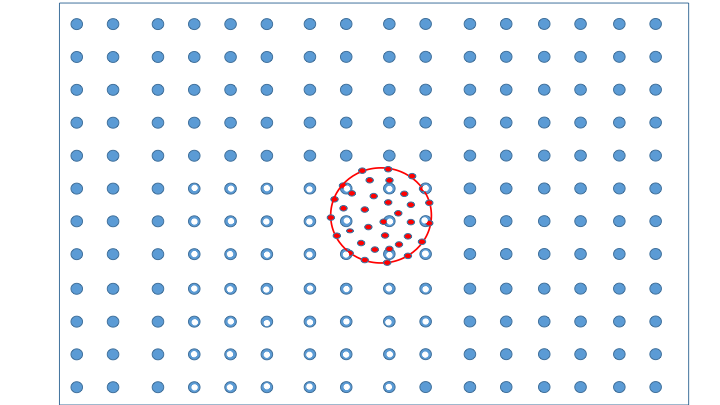
\includegraphics[width=0.6\textwidth]{EESdot}
    \caption{A schematic representation of the ``dual-grid''. Blue dots represent the FFT grid. Red dots represent the $f$-grid for the real-space integration, centered near a particle. Open blue dots are the $\pzp$ FFT-grid points needed for the EES interpolation of the KS states.} 
    \label{fig:EESdot}
\end{figure}


We denote these $\pzp$ points as the set  $\hsJp$ following the notation used above for the density interpolation. Here, the width factors are 

\begin{equation}
\begin{split}
\zeta_{\Psi} &= \frac{2\Rpc}{\Delta^{(\Psi)}}\\
\zeta_{n} &= \frac{2\Rpc}{\Delta^{(n)}}\\
\end{split}
\end{equation}

where $\Delta^{(\Psi)}$ and $\Delta^{(n)}$ are the spacing of the $\Psi$-EES FFT grid and the $n$-EES FFT grid, respectively, assuming for simplicity a cubic simulation cell. Here, we also have a set of points for $\zeta = 0$ for both grids. The utility is that the $\pzp$ or $\pzn$ is independent of system size as is $N_f$.\\

Inserting the above result into Eq.\eqref{eq:fmaster},
\begin{equation}\label{eq:n1rfEES}
\begin{split}
n_J^{(\rP\ 1,\rEES)}(\br_f)
&= \Delta p(\br_f)\sum_I \left[Z_{IJ}^{(\rS,\rEES)*}\Psi_I^{(\rS,\rEES)}(\br_f+\bR_J)  + Z_{IJ}^{(\rS,\rEES)}\Psi_I^{(\rS,\rEES)*}(\br_f+\bR_J) \right] \\
&= \Delta p(\br_f)\sum_I \left[Z_{IJ}^{(\rS,\rEES)*} \sum_{\hat \bs}^{\NFFTpEES} \sum_{\bk} \Mp(\bu_{Jf}-\hat \bs)\delta_{\hat \bs,\bl_{Jf}-\bk} \Psi_I^{(\rS,D)}(\hs)\right] \\
&+ \Delta p(\br_f)\sum_I \left[Z_{IJ}^{(\rS,\rEES)} \sum_{\hat \bs}^{\NFFTpEES} \sum_{\bk} \Mp(\bu_{Jf}-\hat \bs)\delta_{\hat \bs,\bl_{Jf}-\bk} \Psi_I^{(\rS,\rD)*}(\hat \bs)\right] \\
& = \Delta p(\br_f)\sum_{\hat \bs}^{\NFFTpEES} \sum_{\bk} \Mp(\bu_{Jf}-\hat \bs)\delta_{\hat \bs,\bl_{Jf}-\bk} \left(\Psi_J^{(\rS,Z,D)}(\hs)+ \rcc\right) \\
& =\sum_{\hsJp}^{\pzp} \left(\Psi_J^{(\rS,Z,D)}(\hs)+ \rcc\right)\sum_{\bk} \Mp(\bu_{Jf}-\hat \bs) \delta_{\hat \bs,\bl_{Jf}-\bk}\Delta p(\br_f)\\
&=\sum_{\bk} \left(\Psi_J^{(\rS,Z,D)}(\hs)+ \rcc\right) \Mp(\bu_{Jf}-\hat \bs) \Delta p(\br_f)\big|_{\hs=\bl_{Jf}-\bk}\hsinJp \\
\end{split}
\end{equation}

The Kronecker delta restricts the $\hs$ to the $\pzp$ points around atom $J$ as shown in Fig.\ref{fig:EESdot} and hence the
\begin{equation}
\Psi_J^{(\rS,Z,D)}(\hat \bs)=\sum_I Z_{IJ}^{(\rS,\rEES)*} \Psi_I^{(\rS,D)}(\hs) \hsinJp\\
\end{equation}

are only computed at this restricted set of points -- not on the full set of $\NFFTpEES$ points. \\

To compute $n_J^{(\rP\ 1,\rEES)}(\br_f)$, we
\begin{enumerate}
\item Create $\ol \Psi_I^{(\rS,D)}(\bg)$ by multiplying $\Dpg\psigs$. $\NgKS \NKS \sim N^2$.
\item Perform a 3DFFT on the result to get $\Psi_I^{(\rS,D)}(\hs)$. $\NKS\NFFTp \rl \NFFTp \sim N^2 \rl N$.
\item For every particle $J$, we compute the $\Psi_J^{(\rS,Z,D)}(\hat \bs)$ and $\Psi_J^{(\rS,Z,D)*}(\hat \bs)$ by summing over the KS states only on the $\pzp$ grid points around $\bR_J$ needed. $\NKS N \pzp \sim N^2$.
\item For every $J$, $f$, we compute $n_J^{(\rP\ 1,\rEES)}(\br_f)$ by summing over the weight in Eq.\eqref{eq:n1rfEES}. $N N_f p^3 \sim N$.
\end{enumerate}

The derivative w.r.t. $\psigsc$ is
\begin{equation}\label{eq:dn1rfdp}
\begin{split}
\frac{\p n_J^{(\rP\ 1,\rEES)}(\br_f)}{\p \psigsc}
&= \Delta p(\br_f)\sum_{\hat \bs}^{\NFFTpEES} \sum_{\bk} \Mp(\bu_{Jf}-\hat \bs)\delta_{\hat \bs,\bl_{Jf}-\bk}\\
&\times \left[\frac{\p \Psi_J^{(\rS,Z,D)}(\hs)}{\p \psigsc}+ \frac{\p \Psi_J^{(\rS,Z,D)*}(\hs)}{\p \psigsc}\right]\\
\end{split}
\end{equation}

Below, we show how to split the derivative into 2 useful parts labeled  $(\rP\ 1,a,\rEES)$ and $(\rP\ 1,b,\rEES)$. The labels should not be taken literally because parts $a$ and $b$ do not arise from splitting up the density itself.

\begin{equation}
\begin{split}
\frac{\p n_J^{(\rP\ 1,\rEES)}(\br_f)}{\p \psigsc} &= \frac{\p n_J^{(\rP\ 1,a,\rEES)}(\br_f)}{\p \psigsc} + \frac{\p n_J^{(\rP\ 1,b,\rEES)}(\br_f)}{\p \psigsc}
\end{split}
\end{equation}


The splitting of $a$, $b$ parts here will be used for similar terms in this note. where part $a$ is
\begin{equation}\label{eq:dZSDdpsi}
\begin{split}
\frac{\p \Psi_J^{(\rS,Z,D)}(\hs)}{\p \psigsc}
&= \sum_{I'} \frac{\p Z_{I'J}^{(\rS,
\rEES)*}}{\p \psigsc} \Psi_{I'}^{(\rS,D)}(\hat \bs)\hsinJp \\
&= \Psi_{I}^{(\rS,D)}(\hat \bs)\frac{\p Z_{IJ}^{(\rS,\rEES)*}}{\p \psigsc}\hsinJp\\
&= \frac{1}{\sqrt{V}} \Dpgc \tilde p^{(\rS)*}(\bg) \Psi_{I}^{(\rS,\rD)}(\hat \bs) \\
&\ \ \ \ \ \ \times \left\{\sum_{\hat \bs'}^{\NFFTpEES} \re^{-2\pi i\gcpEES \cdot \hat\bs'} \left[\sum_{\bk} \Mp(\bu_{J}-\hat \bs') \delta_{\hat \bs',\bl_J-\bk}\right]\right\} \hsinJp \\
\end{split}
\end{equation}

Part $b$, which is NOT simply ``complex conjugate'' of part $a$, can be evaluated as
\begin{equation}\label{eq:dZSDcdpsi}
\begin{split}
\frac{\p \Psi_J^{(\rS,Z,D)*}(\hs)}{\p \psigsc}
&= \sum_{I'} \frac{\p \Psi_{I'}^{(\rS,D)*}(\hat \bs)}{\p \psigsc} Z_{I'J}^{(\rS,\rEES)}\hsinJp \\
&= Z_{IJ}^{(\rS,\rEES)}\frac{\p \Psi_{I}^{(\rS,D)*}(\hat \bs)}{\p \psigsc} \hsinJp \\
& = \frac{1}{\sqrt V} \Dpgc  Z_{IJ}^{(\rS,\rEES)}  \re^{-\igcs}  \hsinJp \\
\end{split}
\end{equation}

Further simplification requires embedding the result in the full energy derivative.

\subsection{Computing $n_J^{(\rP\ 2,\rEES)}(\br_f)$}

Next, we compute
\begin{equation} \label{eq:n2rf}
n_J^{(\rP\ 2,\rEES)}(\br_f)= \Delta p^2(\br_f) Z_J^{(\rS,2,\rEES)}
\end{equation}

where $\Delta p^2(\br_f)$ is precomputed and $Z_{J}^{(\rS,2,\rEES)} = \sum_I Z_{IJ}^{(\rS,\rEES)*}Z_{IJ}^{(\rS,\rEES)}$.

\begin{enumerate}
\item $Z_{IJ}^{(\rS,\rEES)}$ and $Z_{IJ}^{(\rS,\rEES)*}$ are calculated and stored from previous steps. $ \sim N^2 \rl N$.
\item For every $I$ and $J$, sum over $Z_{J}^{(\rS,2,\rEES)} = \sum_I Z_{IJ}^{(\rS,\rEES)*}Z_{IJ}^{(\rS,\rEES)}$ to get $Z_{J}^{(\rS,2,\rEES)}$. $\NKS N \sim N^2$.
\item For every $f$ and $J$, evaluate $n_J^{(\rP\ 2,\rEES)}(\br_f)$ as in Eq.\eqref{eq:n2rf}. $N_f N \sim N$.
\end{enumerate}

The derivative w.r.t. $\psigsc$ is
\begin{equation} \label{eq:dn2dpsi}
\begin{split}
\frac{\p n_J^{(\rP\ 2,\rEES)}(\br_f)}{\p \psigsc}
&= \Delta p^2(\br_f)\sum_{I'}\frac{\p Z_{I'J}^{(\rS,\rEES)*}}{\p \psigsc} Z_{I'J}^{(\rS,\rEES)} \\
&= \Delta p^2(\br_f) \frac{1}{\sqrt{V}}\sum_{\hat \bs}^{\NFFTpEES} \sum_{\bk} \Mp(\bu_{J}-\hat \bs) \Dpgc \tilde p^{(\rS)*}(\bg)\re^{-2\pi i\gcpEES \cdot \hat\bs} \delta_{\hat \bs,\bl_J-\bk} Z_{IJ}^{(\rS,\rEES)}\\ 
&= \Dpgc \tilde p^{(\rS)*}(\bg) \Delta p^2(\br_f)\frac{1}{\sqrt{V}}\sum_{\hat \bs}^{\NFFTpEES}\left\{ \sum_\bk \re^{-2\pi i\gcpEES \cdot \hat\bs} \left[ Z_{IJ}^{(\rS,\rEES)} \Mp(\bu_{J}-\hat \bs)\delta_{\hat \bs,\bl_J-\bk} \right] \right\}\\
\end{split}
\end{equation}


Note that it is sometimes convenient to write
\begin{equation}
n_J^{(\rcore,\rEES)}(\br_f) = n_J^{(\rP\ 1,\rEES)}(\br_f)+ n_J^{(\rP\ 2,\rEES)}(\br_f)
\end{equation}



\newpage

\section{PAW local electron-ion energy $E^{(\rlo)}$}
The local energy term of PAW can be split into a short term and a long term using the Ewald identity, $\mathrm{erf}(a)+\mathrm{erfc}(a)=1$.
\begin{equation}
\begin{split}
E^{(\rlo)}
&=E^{(\rlo,\rshort)}+E^{(\rlo,\rlong)} \\
&=\int \rd \br n^{(\rtot)}(\br) \sum_K\phi_K^{(\rlo,\rshort)}(\br) \\
& +\int \rd \br n^{(\rtot)}(\br) \sum_K\phi_K^{(\rlo,\rlong)}(\br)
\end{split}
\end{equation}
where
\begin{equation}
\begin{split}
\phi_K^{(\rlo,\rshort)}(\br)&=-eQ_K\frac{\rerfc(\alpha|\br-\bR_K|)}{|\br-\bR_K|} \\
\phi_K^{(\rlo,\rlong)}(\br)&=-eQ_K\sum_\bm \frac{\rerf(\alpha|\br-\bR_K+\bm \bh|)}{|\br-\bR_K+\bm\bh|}
\end{split}
\end{equation}
The definition of $\al$ is given in Sec.\ref{Sec:parameters}, and is selected such that the short range interaction can be evaluated accurately using only the 1st image..


\subsection{Short range electron-ion interaction energy}
Note that if nearest neighbors are included in the short-range potential (short range cut radius covers multiple atoms around $J$), 
The short range local energy can be evaluted as
\begin{equation} \label{eq:locshort}
\begin{split}
E^{(\rlo,\rshort)}
&= \int \rd \br n^{(\rtot)}(\br) \sum_K\phi_K^{(\rlo,\rshort)}(\br)\\
&= E^{(\rS,\rlo,\rshort)} \\
& + \int \rd\br n^{(\rP\ 1)}(\br)\sum_K\phi^{(\rlo,\rshort)}(\br)\\
& + \int \rd\br  n^{(\rP\ 2)}(\br) \sum_K\phi^{(\rlo,\rshort)}(\br)\\
&= E^{(\rS,\rlo,\rshort)} \\
& - \int_{D(\Rpc)} \rd\br \sum_J n^{(\rP\ 1)}(\br+\bR_J)\sum_{<K>_{J,\rNN}}eQ_K\frac{\rerfc(\alpha|\br-\bR_{KJ}|)}{|\br-\bR_{KJ}|} \\
&- \int_{D(\Rpc)} \rd\br \sum_J n^{(\rP\ 2)}(\br+\bR_J)\sum_{<K>_{J,\rNN}}eQ_K\frac{\rerfc(\alpha|\br-\bR_{KJ}|)}{|\br-\bR_{KJ}|} \\
&= E^{(\rS,\rlo,\rshort)} + E^{(\rP\ 1,\rlo,\rshort)} + E^{(\rP\ 2,\rlo,\rshort)}
\end{split}
\end{equation}

Using the EES structure factor $\ol S^{(\rCo,n,\rEES)}(\bg)$, the EES short range smooth local electron-ion interaction is
\begin{equation}
E^{(\rS,\rlo,\rshort,\rEES)} = -\frac{e}{V}\sum_{\bg \neq 0}^\Gc \ol S^{(\rCo,n,\rEES)}(\bg)\overline{n}^{(\rS)}(\bg) \ol \chi^{(\rshort)}(\bg)
\end{equation}

Here, $<K>_{J,\rNN}$ indicates the particles with $|\br-\bR_{KJ}| < \Rc$ where $\Rc$ is the short range cutoff enable by the Ewald approach -- See Eq.\eqref{eq:Rcdef} for the definition of $\Rc$.\\

Introducing the $f$-grid quadrature and the EES approximations to the density yields

\begin{equation} \label{eq:locshortEES12}
\begin{split}
E^{(\rP\ 1,\rlo,\rshort,\rEES)}
&= - \sum_f w_f \sum_J n_J^{(\rP\ 1,\rEES)}(\br_f)\sum_{<K>_{J,\rNN}}eQ_K\frac{\rerfc(\alpha|\br_f-\bR_{KJ}|)}{|\br_f-\bR_{KJ}|} \\
E^{(\rP\ 2,\rlo,\rshort,\rEES)}
&= - \sum_f w_f \sum_J n_J^{(\rP\ 2,\rEES)}(\br_f)\sum_{<K>_{J,\rNN}}eQ_K\frac{\rerfc(\alpha|\br_f-\bR_{KJ}|)}{|\br_f-\bR_{KJ}|} \\
\end{split}
\end{equation}

We denote
\begin{equation}
\phi_J^{(\rcore,\rlo,\rshort,\rNN)}(\br_f) = \sum_{<K>_{J,\rNN}}eQ_K\frac{\rerfc(\alpha|\br_f-\bR_{KJ}|)}{|\br_f-\bR_{KJ}|}
\end{equation}


After $n_J^{(\rP\ 1,\rEES)}(\br_f)$ are created in order $\sim N^2 \rl N$ and stored as described above, the sums in Eq.\eqref{eq:locshortEES12} can be performed in order $NN_{\rNN}N_f \sim N$.\\

To evaluate $E^{(\rP\ 1,\rlo,\rshort,\rEES)}$ and $E^{(\rP\ 2,\rlo,\rshort,\rEES)}$ on a computer, we
\begin{enumerate}
\item $n_J^{(\rP\ 1,\rEES)}(\br_f)$ and $n_J^{(\rP\ 2,\rEES)}(\br_f)$ created and stored in previous steps.
\item For every grid point $f$ and every atom $J$, we compute the short range local potential $\phi_J^{(\rcore,\rlo,\rshort,\rNN)}(\br_f)$ by summing over all the nearest neighbors. $NN_{\rNN}N_f \sim N$.
\item Summing over $J$ and $f$ in Eq.\eqref{eq:locshortEES12} to calculated the energies. $NN_f \sim N$.
\end{enumerate}


The derivative of $\sum_J \phi_J^{(\rcore,\rlo,\rshort,\rNN)}(\br_f)$ w.r.t. $\RJb$ is 
\begin{equation}\label{eq:dphishortNNdR}
\begin{split}
\frac{\p }{\p \RJb}\sum_{J'} \phi_{J'}^{(\rcore,\rlo,\rshort,\rNN)}(\br_f)
&= \frac{\p }{\p \RJb} \sum_{J'} \sum_{<K \neq J'>_{\rNN}}eQ_K\frac{\rerfc(\alpha|\br_f-\bR_{KJ'}|)}{|\br_f-\bR_{KJ'}|} \\
&= \sum_{<K\neq J>_{\rNN}}eQ_K\frac{\p }{\p \RJb}\frac{\rerfc(\alpha|\br_f-\bR_{KJ}|)}{|\br_f-\bR_{KJ}|} + \sum_{<J \neq J'>}eQ_J\frac{\p }{\p \RJb}\frac{\rerfc(\alpha|\br_f-\bR_{JJ'}|)}{|\br_f-\bR_{JJ'}|}\delta_{J\ \rNN\ \mathrm{of}\ J'} \\
&= 2 \sum_{<K\neq J>_{\rNN}}eQ_K \frac{\p |\br_f-\bR_{KJ}|}{\p \RJb} \left[\frac{\p} {\p |\br_f-\bR_{KJ}|} \frac{\rerfc(\alpha|\br_f-\bR_{KJ}|)}{|\br_f-\bR_{KJ}|}\right]\\
&= 2\sum_{<K\neq J>_{\rNN}}eQ_K \frac{\p \left[ \sum_{\beta'} \left(r_{f\beta'}-R_{J,\beta'}+R_{K,\beta'}\right)^2\right]^{1/2}}{\p \RJb}\\
&\ \ \ \ \ \ \ \ \ \ \times \left[\frac{\p} {\p x} \frac{\rerfc(\alpha x)}{x}\right]\bigg|_{x=|\br_f-\bR_{KJ}|}\\
&= 2\sum_{<K\neq J>_{\rNN}}eQ_K \frac{\p \left[ \sum_{\beta'} \left(r_{f\beta'}-R_{J,\beta'}+R_{K,\beta'}\right)^2\right]^{1/2}}{\p \RJb}\\
&\ \ \ \ \ \ \ \ \ \ \times \left[\frac{\p} {\p x} \frac{\rerfc(\alpha x)}{x}\right]\bigg|_{x=|\br_f-\bR_{KJ}|}\\
&= 2\sum_{<K\neq J>_{\rNN}}eQ_K \left[-\frac{r_{f\beta}-R_{KJ,\beta}}{|\br_f-\bR_{KJ}|}\right]\left[\frac{\p}{\p x} \frac{2}{\sqrt{\pi}}\int_{\al x}^{\infty} \re^{-t^2} \rd t\right]\bigg|_{x=|\br_f-\bR_{KJ}|}\\
&= 2\sum_{<K\neq J>_{\rNN}}eQ_K \left[-\frac{r_{f\beta}-R_{KJ,\beta}}{|\br_f-\bR_{KJ}|}\right]\left[-\frac{2\al}{\sqrt{\pi}}\re^{-(\alpha|\br_f-\bR_{KJ}|)^2}\right]\\
&= 2\sum_{<K\neq J>_{\rNN}}eQ_K \left(\frac{2\al}{\sqrt{\pi}} \right)\frac{\left(r_{f\beta}-R_{KJ,\beta}\right)}{|\br_f-\bR_{KJ}|}\re^{-(\alpha|\br_f-\bR_{KJ}|)^2}\\
\end{split}
\end{equation}

Later we use this result to compute the force on the atoms from local short electron-ion interaction.


\subsection{Long range electron-ion interaction energy}
The long range term can be evaluted as
\begin{equation} \label{eq:lloc}
\begin{split}
E^{(\rlo,\rlong)}
&= \int \rd \br n^{(\rtot)}(\br) \sum_K\phi_K^{(\rlo,\rlong)}(\br)\\
&= E^{(\rS,\rlo,\rlong)} \\
& + \sum_{K}\sum_{\bf{m}=-\infty}^\infty \int \rd\br \phi^{(\rlo,\rlong)}(\br-\bR_{K}+\bm\bh) n^{(\rP\ 1)}(\br)\\
& + \sum_{K}\sum_{\bf{m}=-\infty}^\infty \int \rd\br \phi^{(\rlo,\rlong)}(\br-\bR_{K}+\bm\bh) n^{(\rP\ 2)}(\br) \\
\end{split}
\end{equation}

Using the Poisson summation formula yields
\begin{equation}
\begin{split}
E^{(\rlo,\rlong)}
&= E^{(\rS,\rlo,\rlong)} \\
&+ \frac{1}{V} \sum_\bg^\Gc \sum_{K} \wt \phi_K^{(\rlo,\rlong)} (\bg)\int \rd\br \re^{i\bg\cdot(\br-\bR_{K})}n^{(\rP\ 1)}(\br) \\
&+ \frac{1}{V} \sum_\bg^\Gc \sum_{K} \wt \phi_K^{(\rlo,\rlong)} (\bg)\int \rd\br \re^{i\bg\cdot(\br-\bR_{K})}n^{(\rP\ 2)}(\br) \\
\end{split}
\end{equation}

Simplifying,
\begin{equation}
\begin{split}
E^{(\rlo,\rlong)}
& = E^{(\rS,\rlo,\rlong)} \\
& - \frac{e}{V} \sum_{\bg \neq 0}^{\Gc} \frac{4\pi}{g^2} \rexp\left(-\frac{g^2}{4\alpha^2}\right) \left(\sum_{K} Q_K \re^{-\ibgR_{K}}\right) \ol n^{(\rP\ 1)}(\bg)\\
& - \frac{e}{V} \sum_{\bg \neq 0}^{\Gc} \frac{4\pi}{g^2} \rexp\left(-\frac{g^2}{4\alpha^2}\right) \left(\sum_{K} Q_K \re^{-\ibgR_{K}}\right) \ol n^{(\rP\ 2)}(\bg)\\
&+ \left\{\bg=0\ \mathrm{terms}\right\}\\
& = \left[ E^{(\rS,\rlo,\rlong)} + \frac{e\pi}{V \alpha^2} \ol S^{(\rCo,n)}(0) \ol n^{(\rS)}(0)\right] \\
&+ \left[-\frac{e}{V} \sum_{\bg \neq 0}^{\Gc} \ol \chi^{(\rlong)}(\bg)  \ol S^{(\rCo,n)}(\bg) \ol n^{(\rP\ 1)}(\bg)+ \frac{e\pi}{V \alpha^2} \ol S^{(\rCo,n)}(0) \ol n^{(\rP\ 1)}(0)\right] \\
&+ \left[-\frac{e}{V} \sum_{\bg \neq 0}^{\Gc} \ol \chi^{(\rlong)}(\bg)  \ol S^{(\rCo,n)}(\bg) \ol n^{(\rP\ 2)}(\bg)+ \frac{e\pi}{V \alpha^2} \ol S^{(\rCo,n)}(0) \ol n^{(\rP\ 2)}(0)\right] \\
&= E^{(\rS,\rlo,\rlong)} + E^{(\rP\ 1,\rlo,\rlong)}  + E^{(\rP\ 2,\rlo,\rlong)}
\end{split}
\end{equation}


where
\begin{equation} \label{eq:llocdef}
\begin{split}
\ol \chi^{(\rlong)}(\bg) &= \frac{4\pi}{g^2} \rexp\left(-\frac{g^2}{4\alpha^2}\right) \\
\ol S^{(\rCo,n)}(\bg) &= \sum_J Q_J\re^{-\ibgR_J} \\
\ol n^{(\rP\ 1)}(\bg) &= \int_{\rD(\bh)}  \rd \br \re^{-\ibgr} n^{(\rP\ 1)}(\br) \\
\ol n^{(\rP\ 2)}(\bg) &= \int_{\rD(\bh)}  \rd \br \re^{-\ibgr} n^{(\rP\ 2)}(\br) \\
\end{split}
\end{equation}

Next, we use Eq.\eqref{eq:n1rf} and Eq.\eqref{eq:n2rf} and EES interpolation to determine the Fourier coefficients of the core densities,
\begin{equation}
\begin{split}
\ol n^{(\rP\ 1)}(\bg) 
&= \int_{\rD(\bh)}  \rd \br \re^{-\ibgr} n^{(\rP\ 1)}(\br)\\
&= \int_{\rD(\Rpc)}  \rd \br \left[\sum_J \re^{-i\bg\cdot(\br+\bR_J)} n^{(\rP\ 1)}(\br+\bR_J)\right]\\
\ol n^{(\rP\ 1,M,\rEES)}(\bg) 
&= \sum_f w_f \left[\sum_J \re^{-i\bg\cdot(\br_f+\bR_J)}n_J^{(\rP\ 1,\rEES)}(\br_f) \right] + O(\mathrm{grid\ and\ EES\ error}) \\
\end{split}
\end{equation}

Apply Eq.\eqref{eq:fmaster} on the density EES- grid,
\begin{equation} \label{eq:n1gEES}
\begin{split}
\re^{i\bg\cdot(\br_f+\bR_J)}
  & = D_p^{(n)}(\bg)\sum_{\hat \bs}^{\NFFTnEES} \sum_{\bk} \re^{2\pi i\gcnEES \cdot \hat\bs} M_p^{(n)}(\bu_{Jf}-\hat \bs)\delta_{\hat \bs,\bl_{Jf}-\bk} \\
 \ol n^{(\rP\ 1,M,\rEES)}(\bg)
 &=  \sum_f w_f \left\{\sum_J \left[\Dng\sum_{\hat \bs}^{\NFFTnEES} \sum_{\bk} \re^{-2\pi i\gcnEES \cdot \hat\bs} M_p^{(n)}(\bu_{Jf}-\hat \bs)\delta_{\hat \bs,\bl_{Jf}-\bk}\right] n_J^{(\rP\ 1,\rEES)}(\br_f) \right\} \\
 &= D_p^{(n)}(\bg)\sum_{\hat \bs}^{\NFFTnEES} \re^{-2\pi i\gcnEES \cdot \hat\bs}\left\{\sum_J \left[ \sum_f w_f n_J^{(\rP\ 1,\rEES)}(\br_f) \sum_{\bk}  M_p^{(n)}(\bu_{Jf}-\hat \bs)\delta_{\hat \bs,\bl_{Jf}-\bk}\right] \right\}\\
 &= D_p^{(n)}(\bg)\sum_{\hat \bs}^{\NFFTnEES} \re^{-2\pi i\gcnEES \cdot \hat\bs} n^{(\rP\ 1,M,\rEES)}(\hat \bs)\\
 &= \Dng \FFTniEES \left[ n^{(\rP\ 1,M,\rEES)}(\hat \bs), \Gc \right]\\
\end{split}
\end{equation}
where
\begin{equation}
\begin{split}
n_J^{(\rP\ 1,M,\rEES)}(\hs) &=\sum_f w_f n_J^{(\rP\ 1,\rEES)}(\br_f) \sum_{\bk}  M_p^{(n)}(\bu_{Jf}-\hat \bs)\big|_{\hs=\bl_{Jf}-\bk} \hsinJn\\
n^{(\rP\ 1,M,\rEES)}(\hat \bs) &= \sum_J \sum_{\hspJn}^{\pzn} n_J^{(\rP\ 1,M,\rEES)}(\hs') \delta_{\hs,\hs'} \hsinnEES\\
\end{split}
\end{equation}

The  $\ol n^{(\rP\ 2,M,\rEES)}(\bg)$ can be obtained by a 3DFFT on 

\begin{equation} \label{eq:n2gEES}
\begin{split}
 \ol n^{(\rP\ 2,M,\rEES)}(\bg)
 &= \Dng \FFTniEES \left[ n^{(\rP\ 2,M,\rEES)}(\hat \bs), \Gc \right]
\end{split}
\end{equation}
where
\begin{equation}
\begin{split}
n_J^{(\rP\ 2,M,\rEES)}(\hat \bs) &=\sum_f w_f n_J^{(\rP\ 2,\rEES)}(\br_f) \sum_{\bk}  M_p^{(n)}(\bu_{Jf}-\hat \bs)\delta_{\hat \bs,\bl_{Jf}-\bk} \hsinJn\\
n^{(\rP\ 2,M,\rEES)}(\hat \bs) &= \sum_J \sum_{\hspJn}^{\pzn} n_J^{(\rP\ 2,M,\rEES)}(\hs') \delta_{\hs,\hs'} \hsinnEES\\
\end{split}
\end{equation}

We can combine the $\bg$-space $(\rP\ 1)$ and $(\rP\ 2)$ densities
\begin{eqnarray}
\ol n^{(\rcore,\rEES)}(\bg) &=& \ol n^{(\rP\ 1,M,\rEES)}(\bg)+\ol n^{(\rP\ 2,M,\rEES)}(\bg)\\
\ol n^{(\rtot,\rEES)}(\bg) &=& \ol n^{(\rS)}(\bg)+\ol n^{(\rcore,\rEES)}(\bg)
\end{eqnarray}



After EESing everything, we have

\begin{equation}
\begin{split}
E^{(\rlo,\rlong,\rEES)}
& = \left[E^{(\rS,\rlo,\rlong,\rEES)} + \frac{e\pi}{V \alpha^2} \ol S^{(\rCo,n,\rEES)}(0) \ol n^{(\rS)}(0)\right] \\
&+ \left[-\frac{e}{V} \sum_{\bg \neq 0}^{\Gc} \ol \chi^{(\rlong)}(\bg)  \ol S^{(\rCo,n,\rEES)}(\bg) \ol n^{(\rP\ 1,M,\rEES)}(\bg) + \frac{e\pi}{V \alpha^2} \ol S^{(\rCo,n,\rEES)}(0) \ol n^{(\rP\ 1,M,\rEES)}(0)\right]\\
&+ \left[-\frac{e}{V} \sum_{\bg \neq 0}^{\Gc} \ol \chi^{(\rlong)}(\bg)  \ol S^{(\rCo,n,\rEES)}(\bg) \ol n^{(\rP\ 2,M,\rEES)}(\bg) + \frac{e\pi}{V \alpha^2} \ol S^{(\rCo,n,\rEES)}(0) \ol n^{(\rP\ 2,M,\rEES)}(0)\right]\\
&= E^{(\rS,\rlo,\rlong,\rEES)} + E^{(\rP\ 1,\rlo,\rlong,\rEES)}  + E^{(\rP\ 2,\rlo,\rlong,\rEES)}
\end{split}
\end{equation}


To compute $E^{(\rP\ 1,\rlo,\rlong,\rEES)}$ and $E^{(\rP\ 2,\rlo,\rlong,\rEES)} $, we
\begin{enumerate}
\item $n_J^{(\rP\ 1,\rEES)}(\br_f)$ is created and stored in $\sim N^2 \rl N$ previously.
\item Create $n^{(\rP\ 1,M,\rEES)}(\hat \bs)$ in $N_fNp^3 \sim N$.
\item 3DFFT on $n^{(\rP\ 1,M,\rEES)}(\hat \bs)$. $\NFFTn \rl \NFFTn \sim N \rl N$.
\item Multiply the result with $D_p^{(n)}$ to obtain $\ol n^{(\rP\ 1,M,\rEES)}(\bg)$. $\Ngn \sim N$.
\item Repeat the steps above to get $\ol n^{(\rP\ 2,\rEES)}(\bg)$.
\item $\ol S^{(\rCo,n,\rEES)}(\bg)$ is created and stored in $\sim N \rl N$.
\item Multiply $\ol \chi^{(\rlong)}(\bg)  \ol S^{(\rCo,n,\rEES)}(\bg) \ol n^{(\rP\ 1,M,\rEES)}(\bg)$ and sum over $\bg$ to get $E^{(\rP\ 1,\rlo,\rlong,\rEES)}$, note that the $\bg$ sum is truncated by $\ol \chi^{(\rlong)}(\bg)$ due to our selection of $\Rc$. $\Ngn \sim N$.
\item Multiply $\ol \chi^{(\rlong)}(\bg)  \ol S^{(\rCo,n,\rEES)}(\bg) \ol n^{(\rP\ 2,M,\rEES)}(\bg)$ and sum over $\bg$ to get $E^{(\rP\ 2,\rlo,\rlong,\rEES)}$, again the $\bg$ sum is truncated by $\ol \chi^{(\rlong)}(\bg)$ due to our selection of $\Rc$. $\Ngn \sim N$.
\end{enumerate}


\subsection{Combined smooth local energy $E^{(\rS,\rlo,\rcomb)}$}
The smooth part can be combined by,
\begin{equation}\label{eq:ElocS}
\begin{split}
E^{(\rS,\rlo,\rcomb,\rEES)}
&= E^{(\rS,\rlo,\rshort,\rEES)} + E^{(\rS,\rlo,\rlong,\rEES)} \\
&= -\frac{e}{V}\sum_{\bg \neq 0}^\Gc \ol S^{(\rCo,n,\rEES)}(\bg)\overline{n}^{(\rS)}(\bg) \left[\ol \chi^{(\rshort)}(\bg)+\ol \chi^{(\rlong)}(\bg) \right] \\
&= -\frac{e}{V}\sum_{\bg \neq 0}^\Gc \frac{4\pi}{g^2} \ol S^{(\rCo,n,\rEES)}(\bg)\overline{n}^{(\rS)}(\bg)
\end{split}
\end{equation}

And we can rewrite $E^{(\rlo,\rEES)}$ as
\begin{equation}\label{eq:ElocSEES} 
\begin{split}
E^{(\rlo,\rEES)}
&= E^{(\rlo,\rshort,\rEES)} +E^{(\rlo,\rlong,\rEES)} \\
&= E^{(\rS,\rlo,\rcomb,\rEES)} + \left[E^{(\rP\ 1,\rlo,\rshort,\rEES)} + E^{(\rP\ 2,\rlo,\rshort,\rEES)}\right] \\
&\ \ \ \ +\left[E^{(\rP\ 1,\rlo,\rlong,\rEES)} + E^{(\rP\ 2,\rlo,\rlong,\rEES)} \right]\\
&= E^{(\rS,\rlo,\rcomb,\rEES)} + E^{(\rcore,\rlo,\rshort,\rEES)}  + E^{(\rcore,\rlo,\rlong,\rEES)}
\end{split}
\end{equation}


To calculate $E^{(\rS,\rlo,\rcomb,\rEES)}$ on a computer, we
\begin{enumerate}
\item Create $\bg$-space density $\ol{n}^{(\rS)}(\bg)$. $\sim N^2 \rl N$.
\item $\ol S^{(\rCo,n,\rEES)}(\bg)$ created and stored. $\sim N\rl N$.
\item For every $\bg$, multiply each term in Eq.\eqref{eq:ElocSEES} and perform the sum. $\Ngn \sim N$.
\end{enumerate}

\subsection{Derivatives of the combined smooth energy $E^{(\rS,\rlo,\rcomb,\rEES)}$}
\subsubsection{Derivative with respect to $\psigsc$}
The derivative of the combined smooth part $E^{(\rS,\rlo,\rcomb,\rEES)} = E^{(\rS,\rlo,\rshort,\rEES)} + E^{(\rS,\rlo,\rlong,\rEES)}$ with respect to wavefunction coefficients $\psigsc$ is
\begin{equation}
\begin{split}
\frac{\p E^{(\rS,\rlo,\rcomb,\rEES)}}{ \p \psigsc}
&=  -\frac{e}{V} \frac{\p }{ \p \psigsc}\sum_{\bg' \neq 0}^\Gc \frac{4\pi }{g'^2} \ol S^{(\rCo,n,\rEES)}(\bg')\overline{n}^{(\rS)}(\bg')\\
\end{split}
\end{equation}

Using Eq.\eqref{eq:nSg}, we have
\begin{equation}\label{eq:dnSgdp}
\begin{split}
\frac{\p \ol {n}^{(\rS)}(\bg')}{ \p \psigsc}
&= \frac{1}{\sqrt V} \frac{\p }{ \p \psigsc} \sum_{\hat \bs}^\NFFTn  \sum_{I'}  \left[\sum_{\bg''_c}^{\Gc/2} \overline{\Psi}_{I'}^{(\rS)*}(\bg''_c)  \re^{-2\pi i \gcn'' \cdot \hat \bs}\right] \Psi_{I'}^{(\rS)}(\hat \bs) \re^{-\igpcns} \\
&= \frac{1}{\sqrt V} \sum_{\hat \bs}^\NFFTn   \re^{-\igcns}\Psi_{I}^{(\rS)}(\hat \bs) \re^{-\igpcns}
\end{split}
\end{equation}

Therefore,
\begin{equation}
\begin{split}
\frac{\p E^{(\rS,\rlo,\rcomb,\rEES)}}{ \p \psigsc}
&= -\frac{e}{V} \sum_{\bg' \neq 0}^\Gc \frac{4\pi }{g'^2} \ol S^{(\rCo,n,\rEES)}(\bg')\frac{\p \ol{n}^{(\rS)}(\bg') }{ \p \psigsc}\\
&= -\frac{e}{V} \sum_{\bg' \neq 0}^\Gc \frac{4\pi }{g'^2} \ol S^{(\rCo,n,\rEES)}(\bg')\left[\frac{1}{\sqrt V} \sum_{\hat \bs}^\NFFTn   \re^{-\igcns}\Psi_{I}^{(\rS)}(\hat \bs) \re^{-\igpcns}\right]\\
&= \frac{1}{\sqrt V} \sum_{\hat \bs}^\NFFTn   \re^{-\igcns}\left\{\Psi_{I}^{(\rS)}(\hat \bs) \left[-\frac{e}{V} \sum_{\bg' \neq 0}^{\Gc} \re^{-\igpcns} \frac{4\pi }{g'^2} \ol S^{(\rCo,n,\rEES)}(\bg')\right] \right\}\\
&=  \frac{1}{\sqrt V} \sum_{\hat \bs}^\NFFTn   \re^{-\igcns}\left[\Psi_{I}^{(\rS)}(\hat \bs) \phi^{(W,\rS,\rlo,\rcomb,\chi,S,\rEES)}(\hs)\right] \\
&= \frac{1}{\sqrt V} \FFTni \left[\Psi_{I}^{(\rS)}(\hat \bs) \phi^{(W,\rS,\rlo,\rcomb,\chi,S,\rEES)}(\hs),\hGc \right]
\end{split}
\end{equation}
Note that the convolution requires both $\Psi_{I}^{(\rS)}(\hat \bs)$ and $\phi^{(W,\rS,\rlo,\rcomb,\chi,S,\rEES)}(\hs)$ to be evaluated on the density grid.

The KS potential for the combined smooth local electron-ion interaction is
\begin{equation}\label{eq:Vlocs}
\begin{split}
\phi^{(W,\rS,\rlo,\rcomb,\chi,S,\rEES)}(\hs) 
&= -\frac{e}{V} \sum_{\bg \neq 0}^{\Gc} \re^{-\igcns} \frac{4\pi }{g^2} \ol S^{(\rCo,n,\rEES)}(\bg)\\
&= -\frac{e}{V} \IFFTni \left[\frac{4\pi }{g^2} \ol S^{(\rCo,n,\rEES)}(\bg), \Gc \right] \hsinn
\end{split}
\end{equation}

To calculate $\frac{\p E^{(\rS,\rlo,\rcomb,\rEES)}}{ \p \psigsc}$ on a computer:
\begin{enumerate}
\item $\ol S^{(\rCo,n,\rEES)}(\bg)$ calculated and stored in order $\sim N \rl N$.
\item Perform a 3DFFT in Eq.\eqref{eq:Vlocs} to create $\phi^{(W,\rS,\rlo,\rcomb,\chi,S,\rEES)}(\hs)$. $\NFFTn \rl \NFFTn \sim N \rl N$.
\item For every K-S state $I$, Perform a 3DFFT on $\Psi_{I}^{(\rS)}(\hat \bs) \phi^{(W,\rS,\rlo,\rcomb,\chi,S,\rEES)}(\hs)$. $\NKS \NFFTn \rl \NFFTn \sim N^2 \rl N$. In practice, you collect all the parts of the K-S potential and perform 1 FFT per state, not 1 FFT per term per state.
\end{enumerate}




\subsubsection{Derivative with respect to $\RJa$}
Use Eq.\eqref{eq:sgg}, we can evaluate the derivative,
\begin{equation}\label{eq:dElocdR}
\begin{split}
\frac{\p E^{(\rS,\rlo,\rcomb,\rEES)}}{ \p \RJb}
&= -\frac{e}{V} \frac{\p }{ \p \RJb}\sum_{\bg}^\Gc \frac{4\pi}{g^2} \ol S^{(\rCo,n,\rEES)}(\bg)\overline{n}^{(\rS)}(\bg)\\
&= -\frac{e}{V} \sum_{\bg}^\Gc \frac{4\pi}{g^2} \ol{n}^{(\rS)}(\bg) \Dng \sum_{\hat \bs}^\NFFTnEES \re^{2\pi i\gcnEES \cdot \hat\bs} \left[Q_J \sum_{\bk} \frac{\p M_p^{(3,n)}(\bu_{J}-\hat \bs)\delta_{\hat \bs,\bl_J-\bk}}{\p \RJb}\right] \\
&= Q_J \sum_{\hat \bs}^\NFFTnEES \left[ \sum_{\bk} \frac{\p M_p^{(3,n)}(\bu_{J}-\hat \bs)\delta_{\hat \bs,\bl_J-\bk}}{\p \RJb}\right] \left[-\frac{e}{V} \sum_{\bg}^\Gc \re^{\igcnEESs} \frac{4\pi}{g^2} \ol{n}^{(\rS)}(\bg) \Dng \right] \\
&= Q_J \sum_{\hat \bs}^\NFFTnEES \left[ \sum_{\bk} \frac{\p M_p^{(3,n)}(\bu_{J}-\hat \bs)\delta_{\hat \bs,\bl_J-\bk}}{\p \RJb}\right] \phi^{(R,\rS,\rlo,\rcomb,\chi,D)}(\hs)\\
&= Q_J \left[ \sum_{\bk} \frac{\p M_p^{(3,n)}(\bu_{J}-\hat \bs)}{\p \RJb} \phi^{(R,\rS,\rlo,\rcomb,\chi,D)}(\hs)\right]\big|_{\hat \bs=\bl_J-\bk} \hsinJnzr\\    
\end{split}
\end{equation}

where
\begin{equation}
\begin{split}
\phi^{(R,\rS,\rlo,\rcomb,\chi,D)}(\hs)
&= -\frac{e}{V} \sum_{\bg}^\Gc \re^{\igcnEESs} \frac{4\pi}{g^2} \ol{n}^{(\rS)}(\bg) \Dng\\
&= -\frac{e}{V} \IFFTnEES \left[\frac{4\pi}{g^2} \ol{n}^{(\rS)}(\bg) \Dng, \Gc \right] \hsinn
\end{split}
\end{equation}

To compute $\frac{\p E^{(\rS,\rlo,\rcomb,\rEES)}}{ \p \RJb}$, we
\begin{enumerate}
\item Calculate $\ol \phi^{(R,\rS,\rlo,\rcomb,\chi,D)}(\bg)$ by multiplying $\frac{4\pi}{g^2} \ol{n}^{(\rS)}(\bg) \Dng$ in $\Ngn \sim N$.
\item FFT on $\ol \phi^{(R,\rS,\rlo,\rcomb,\chi,D)}(\bg)$ to get $\phi^{(R,\rS,\rlo,\rcomb,\chi,D)}(\hs)$ in $\NFFTn \rl \NFFTn \sim N\rl N$.
\item For every particle $J$, calculate the force by summing over the last equation in Eq.\eqref{eq:dElocdR}. $3 N p^3 \sim N$.
\end{enumerate}




\newpage
\subsection{Derivatives of the short range core local  energy}
\subsubsection{Derivative with respect to $\psigsc$}
The core (PAW 1 + PAW 2) part short range local energy wavefunction derivative can be written as
\begin{equation}
\frac{\p E^{(\rcore,\rlo,\rshort,\rEES)} }{\p \psigsc}
= \frac{\p E^{(\rP\ 1,\rlo,\rshort,\rEES)}}{\p \psigsc}
+ \frac{\p E^{(\rP\ 2,\rlo,\rshort,\rEES)}}{\p \psigsc}
\end{equation}


The derivative related to $n_J^{(\rP\ 1,\rEES)}(\br_f)$ can be written as

\begin{equation}
\begin{split}
\frac{\p E^{(\rP\ 1,\rlo,\rshort,\rEES)}}{\p \psigsc}
&= - \sum_f w_f \sum_J \frac{\p n_J^{(\rP\ 1,\rEES)}(\br_f)}{\p \psigsc}\phi_J^{(\rcore,\rlo,\rshort,\rNN)}(\br_f)\\
&= \frac{\p E^{(\rP\ 1,\rlo,\rshort,a,\rEES)}}{\p \psigsc}+\frac{\p E^{(\rP\ 1,\rlo,\rshort,b,\rEES)}}{\p \psigsc} \\
\end{split}
\end{equation}

$\frac{\p n_J^{(\rP\ 1,\rEES)}(\br_f)}{\p \psigsc}$ is split into 2 parts as in Eq.\eqref{eq:dZSDdpsi} and Eq.\eqref{eq:dZSDcdpsi}.\\

Use Eq.\eqref{eq:dn1rfdp}, the $a$ part can be written as,
\begin{equation}
\begin{split}
\frac{\p E^{(\rP\ 1,\rlo,\rshort,a,\rEES)}}{\p \psigsc}
&= \sum_J \sum_{\hsJp}^\pzp \Psi_{I}^{(\rS,D)}(\hat \bs) \left[-\sum_f w_f \Delta p(\br_f) \phi_J^{(\rcore,\rlo,\rshort,\rNN)}(\br_f) \sum_{\bk} \Mp(\bu_{Jf}-\hat \bs)\delta_{\hat \bs,\bl_{Jf}-\bk}\right] \\
&\times \frac{1}{\sqrt{V}} \Dpgc \tilde p^{(\rS)*}(\bg)  \sum_{\hat \bs'}^\NFFTpEES \re^{-2\pi i\gcpEES \cdot \hat\bs'} \left[\sum_{\bk'} \Mp(\bu_{J}-\hat \bs') \delta_{\hat \bs',\bl_J-\bk'}\right] \\
&= \frac{1}{\sqrt{V}} \Dpgc \tilde p^{(\rS)*}(\bg)\sum_{\hat \bs'}^\NFFTpEES \re^{-2\pi i\gcpEES \cdot \hat\bs'} \\
&\ \ \ \ \ \ \times \left[\sum_J Z_{IJ}^{(W,\rP\ 1,\rlo,\rshort,a,\rEES)}\sum_{\bk'} \Mp(\bu_{J}-\hat \bs') \delta_{\hat \bs',\bl_J-\bk'}\right] \\
&= \frac{1}{\sqrt{V}} \Dpgc \tilde p^{(\rS)*}(\bg)\sum_{\hat \bs'}^\NFFTpEES \re^{-2\pi i\gcpEES \cdot \hat\bs'} \left[F_I^{(\rP\ 1,\rlo,\rshort,a,\rEES)}(\hs')\right] \\
&= \Dpgc \tilde p^{(\rS)*}(\bg)\frac{1}{\sqrt{V}} \FFTpiEES \left[F_I^{(W,\rP\ 1,\rlo,\rshort,a,\rEES)}(\hs),\hGc \right] \\
\end{split}
\end{equation}

where
\begin{equation}\label{eq:dElocshortdpterms}
\begin{split}
F_I^{(W,\rP\ 1,\rlo,\rshort,a,\rEES)}(\hs) &= \sum_{J=1}^N Z_{IJ}^{(W,\rP\ 1,\rlo,\rshort,a,\rEES)}\sum_{\bk} \Mp(\bu_{J}-\hat \bs) \delta_{\hat \bs,\bl_J-\bk} \hsinpEES \\
Z_{IJ}^{(W,\rP\ 1,\rlo,\rshort,a,\rEES)} &= \sum_{\hsJp}^{\pzp} \Psi_{I}^{(\rS,D)}(\hat \bs) \phi_J^{(\rP\ 1,\rlo,\rshort,\rEES)}(\hs)\\
\phi_J^{(\rP\ 1,\rlo,\rshort,\rEES)}(\hs) &= -\sum_f w_f \Delta p(\br_f) \phi_J^{(\rcore,\rlo,\rshort,\rNN)}(\br_f) \sum_{\bk} \Mp(\bu_{Jf}-\hat \bs)\delta_{\hs,\bl_{Jf}-\bk} \hsinJp \\
\end{split}
\end{equation}

The cost to evaluate $\phi_J^{(\rP\ 1,\rlo,\rshort,\rEES)}(\hs)$ is $NN_f p^3 \sim N$, and the $\hat \bs$ is restricted to $(p+\zeta)^3$ points around atom $J$. The cost to evaluate $Z_{IJ}^{(W,\rP\ 1,\rlo,\rshort,a,\rEES)}$ is $\NKS N (p+\zeta)^3 \sim N^2$, which is the most expensive scaling of the real space part of the calculation.\\

The $b$ part, which is related to $\Psi_J^{(\rS,Z,D)*}(\hat \bs)$, can be written as,
\begin{equation}
\begin{split}
\frac{\p E^{(\rP\ 1,\rlo,\rshort,b,\rEES)}}{\p \psigsc}
&= - \sum_J \sum_f w_f \Delta p(\br_f) \phi_J^{(\rcore,\rlo,\rshort,\rNN)}(\br_f)\sum_{\hsJp}^\pzp \sum_{\bk} \Mp(\bu_{Jf}-\hat \bs)\delta_{\hat \bs,\bl_{Jf}-\bk} \\
& \times \frac{1}{\sqrt V} \Dpgc  Z_{IJ}^{(\rS,\rEES)}  \re^{-\igcps} \\
&= \frac{1}{\sqrt V} \Dpgc \sum_{\hs}^\NFFTpEES \re^{-\igcps} \left\{\sum_J Z_{IJ}^{(\rS,\rEES)}\left[\sum_{\hspJp}^\pzp \phi_J^{(\rP\ 1,\rlo,\rshort,\rEES)}(\hs') \delta_{\hs,\hs'}\right]\right\}\\
&= \frac{1}{\sqrt V} \Dpgc \FFTpiEES \left[F_I^{(W,\rP\ 1,\rlo,\rshort,b,\rEES)}(\hs),\hGc\right]\\
\end{split}
\end{equation}

where 
\begin{equation}
\begin{split}
F_I^{(W,\rP\ 1,\rlo,\rshort,b,\rEES)}(\hs)&= \sum_J Z_{IJ}^{(\rS,\rEES)}\left[\sum_{\hspJp}^\pzp \phi_J^{(\rP\ 1,\rlo,\rshort,\rEES)}(\hs') \delta_{\hs,\hs'}\right]\hsinpEES\\
\end{split}
\end{equation}

To evaluate $\frac{\p E^{(\rP\ 1,\rlo,\rshort,\rEES)}}{\p \psigsc}$ on a computer, we
\begin{enumerate}
\item For every atom $J$, calculate $\phi_J^{(\rP\ 1,\rlo,\rshort,\rEES)}(\hs)$ as in Eq.\eqref{eq:dElocshortdpterms} by summing over $f$ and the EES interpolations points. $\sim$ $NN_fp^3 \sim N$.
\item Add up $\Psi_{I}^{(\rS,D)}(\hat \bs) \phi_J^{(\rP\ 1,\rlo,\rshort,\rEES)}(\hs)$ only on the $\pzp$ atoms around $J$ to get $Z_{IJ}^{(W,\rP\ 1,\rlo,\rshort,a,\rEES)}$. $\sim$ $\NKS N \pzp \sim N^2$.
\item For every KS state $I$, calculate $F_I^{(W,\rP\ 1,\rlo,\rshort,a,\rEES)}(\hs)$ as in Eq.\eqref{eq:dElocshortdpterms} by summing over all the atom $J$ and the EES interpolation points. $\sim$ $\NKS N p^3 \sim N^2$.
\item For every KS state $I$, 3DFFT on $F_I^{(W,\rP\ 1,\rlo,\rshort,a,\rEES)}(\hs)$ on the $(\Psi,\rEES)$ grid to get $\ol F_I^{(\rP\ 1,\rlo,\rshort,a,\rEES)}(\bg)$. $\sim$ $\NKS \NFFTpEES \rl \NFFTpEES \sim N^2 \rl N$.
\item Multiply $\Dpgc \tilde p^{(\rS)*}(\bg) \ol F_I^{(\rlo,\rshort,1,a,\rEES)}(\bg)$ to get the ``$a$'' part of the derivative. $\sim$ $\NKS \Ngp \sim N^2$.
\item For every KS state $I$, sum over $\sum_J Z_{IJ}^{(\rS,\rEES)}\left[\sum_{\hspJp}^\pzp \phi_J^{(\rP\ 1,\rlo,\rshort,\rEES)}(\hs') \delta_{\hs,\hs'}\right]$ on the $\pzp$ points around each atom $J$ to get $F_I^{(W,\rP\ 1,\rlo,\rshort,b,\rEES)}(\hs)$. $\sim$ $\NKS N \pzp \sim N^2$.
\item For every KS state $I$, FFT on $F_I^{(W,\rP\ 1,\rlo,\rshort,b,\rEES)}(\hs)$ to get $\ol F_I^{(\rlo,\rshort,1,b,\rEES)}(\bg)$. $\sim \NKS \NFFTpEES \rl \NFFTpEES \sim N^2 \rl N$.
\item Multiply $\Dpgc \ol F_I^{(\rlo,\rshort,1,b,\rEES)}(\bg)$ to get the ``$b$'' part of the derivative. $\sim$ $\NKS \Ngp \sim N^2$.
\item Add up the ``$a$'' part and the ``$b$'' part.
\end{enumerate}

\vspace{2mm}
The derivative related to $n_J^{(\rP\ 2,\rEES)}(\br_f)$ takes from as follows by using Eq.\eqref{eq:dn2dpsi},
\begin{equation}
\begin{split}
\frac{\p E^{(\rP\ 2,\rlo,\rshort,\rEES)}}{\p \psigsc}
&= - \sum_f w_f \phi_J^{(\rcore,\rlo,\rshort,\rNN)}(\br_f)\sum_J \frac{\p n_J^{(\rP\ 2,\rEES)}(\br_f)}{\p \psigsc} \\
&= - \Dpgc \tilde p^{(\rS)*}(\bg)  \sum_J  \left[\sum_f w_f \Delta p^2(\br_f) \phi_J^{(\rcore,\rlo,\rshort,\rNN)}(\br_f)\right]\\
&\times\frac{1}{\sqrt{V}}\sum_{\hat \bs}^\NFFTpEES \sum_{\bk} \re^{-\igcps} \left[ Z_{IJ}^{(\rS,\rEES)} \Mp(\bu_{J}-\hat \bs)\delta_{\hat \bs,\bl_J-\bk} \right] \\
&= \Dpgc \tilde p^{(\rS)*}(\bg)  \frac{1}{\sqrt{V}}\\
&\times\sum_{\hat \bs}^\NFFTpEES \re^{-\igcps} \left[\sum_J  Z_{IJ}^{(\rS,\rEES)} \phi_J^{(\rP\ 2,\rlo,\rshort)}  \sum_{\bk}  \Mp(\bu_{J}-\hat \bs)\delta_{\hat \bs,\bl_J-\bk} \right] \\
&= \Dpgc\tilde p^{(\rS)*}(\bg)\frac{1}{\sqrt{V}}\sum_{\hat \bs}^\NFFTpEES \re^{-\igcps}F_I^{(W,\rP\ 2,\rlo,\rshort,\rEES)}(\hs) \\
&= \Dpgc\tilde p^{(\rS)*}(\bg)\frac{1}{\sqrt{V}}\FFTpiEES \left[F_I^{(W,\rP\ 2,\rlo,\rshort,\rEES)}(\hs),\hGc \right]\\
\end{split}
\end{equation}

where
\begin{equation}
\begin{split}
F_I^{(W,\rP\ 2,\rlo,\rshort,\rEES)}(\hs) &= \sum_J  Z_{IJ}^{(\rS,\rEES)} \phi_J^{(\rP\ 2,\rlo,\rshort)} \sum_{\bk}  \Mp(\bu_{J}-\hat \bs)\delta_{\hat \bs,\bl_J-\bk} \hsinpEES \\
\phi_J^{(\rP\ 2,\rlo,\rshort)}&= -\sum_f w_f \Delta p^2(\br_f) \phi_J^{(\rcore,\rlo,\rshort,\rNN)}(\br_f) \\
\end{split}
\end{equation}


To evaluate $\frac{\p E^{(\rP\ 2,\rlo,\rshort,\rEES)}}{\p \psigsc}$ on a computer, we
\begin{enumerate}
\item For every atom $J$, calculate $\phi_J^{(\rP\ 2,\rlo,\rshort)}$ by summing over $f$ . $\sim$ $NN_f \sim N$.
\item For every KS state $I$, calculate $F_I^{(W,\rP\ 2,\rlo,\rshort,\rEES)}(\hs)$ by summing over all $J$ and the EES interpolations points in $\NKS Np^3 \sim N^2$.
\item For every KS state $I$, 3DFFT on $F_I^{(W,\rP\ 2,\rlo,\rshort,\rEES)}(\hs)$ on the $(\Psi,\rEES)$ grid to get $\ol F_I^{(\rP\ 2,\rlo,\rshort,\rEES)}(\bg)$. $\sim$ $\NKS \NFFTpEES \rl \NFFTpEES \sim N^2 \rl N$.
\item Multiply $\Dpgc \tilde p^{(\rS)*}(\bg) \ol F_I^{(\rlo,\rshort,2,\rEES)}(\bg)$ in $\NKS \Ngp \sim N^2$.
\end{enumerate}








\subsubsection{Derivative with respect to $\RJa$}
The derivative of $E^{(\rcore,\rlo,\rshort,\rEES)}$ with respect to ion position $\RJb$ can be evaluated as
\begin{equation}\label{eq:dElocshortdR}
\begin{split}
\frac{\p E^{(\rcore,\rlo,\rshort,\rEES)} }{\p \RJb} &=
\sum_{l=1}^2\frac{\p E^{(\rP\ l,\rlo,\rshort,\rEES)} }{\p \RJb}\\
&= - \sum_f w_f \sum_{J'} \phi_{J'}^{(\rshort,\rNN)}(\br_f)\sum_{l=1}^2\frac{\p n_{J'}^{(\rP\ l,\rEES)}(\br_f)}{\p \RJb} \\
&\ \ \ - \sum_f w_f \left[\sum_{l=1}^2 \sum_{J'} n_{J'}^{(\rP\ l,\rEES)}(\br_f)\right]\frac{\p \phi_{J'}^{(\rshort,\rNN)}(\br_f)}{\p \RJb}\\
&= - \sum_f w_f \phi_J^{(\rcore,\rlo,\rshort,\rNN)}(\br_f)\sum_{l=1}^2\frac{\p n_{J}^{(\rP\ l,\rEES)}(\br_f)}{\p \RJb} \\
&\ \ \ - \sum_f w_f  n_{J}^{(\rcore,\rEES)}(\br_f) \frac{\p \phi_J^{(\rcore,\rlo,\rshort,\rNN)}(\br_f)}{\p \RJb} \\
&= \frac{\p E^{(\rcore,\rlo,\rshort,\rA,\rEES)}}{\p \RJb}+\frac{\p E^{(\rcore,\rlo,\rshort,\rB,\rEES)}}{\p \RJb}
\end{split}
\end{equation}

where the derivative of the short range local potential (with nearest neighbors included) is calculated in Eq.\eqref{eq:dphishortNNdR}
\begin{equation}\label{eq:dphiNNJdR}
\frac{\p \phi_J^{(\rcore,\rlo,\rshort,\rNN)}(\br_f)}{\p \RJb}
= 2\sum_{<K\neq J>_{\rNN}}eQ_K \left(\frac{2\al}{\sqrt{\pi}} \right)\frac{\left(r_{f,\beta}-R_{KJ,\beta}\right)}{|\br_f-\bR_{KJ}|}\re^{-(\alpha|\br_f-\bR_{KJ}|)^2}\\
\end{equation}
which can be calculated in $\sim NN_fN_\rNN$. The second term (part ``$\rB$'') of Eq.\eqref{eq:dElocshortdR} can be calculated in $\sim NN_f$. \\

The derivative of $n_{J}^{(\rP\ l,\rEES)}(\br_f)$ can be evaluated as
\begin{equation} \label{eq:dnrfdR}
\begin{split}
\frac{\p n_{J}^{(\rP\ 1,\rEES)}(\br_f)}{\p \RJb}&=\frac{\p n_{J}^{(\rP\ 1,a,\rEES)}(\br_f)}{\p \RJb} + \frac{\p n_{J}^{(\rP\ 1,b,\rEES)}(\br_f)}{\p \RJb}\\
\frac{\p n_{J}^{(\rP\ 1,a,\rEES)}(\br_f)}{\p \RJb} 
&= \Delta p(\br_f)\sum_{\hat \bs}^{\NFFTpEES} \sum_{\bk} \frac{\p \Mp(\bu_{Jf}-\hat \bs)}{\p \RJb}\delta_{\hat \bs,\bl_{Jf}-\bk} \left(\Psi_J^{(\rS,Z,D)}(\hs)+ \rcc\right) \\
\frac{\p n_{J}^{(\rP\ 1,b,\rEES)}(\br_f)}{\p \RJb} 
&= \Delta p(\br_f)\sum_{\hat \bs}^{\NFFTpEES} \sum_{\bk} \Mp(\bu_{Jf}-\hat \bs)\delta_{\hat \bs,\bl_{Jf}-\bk} \\
&\ \ \ \ \ \ \ \ \times \left[\sum_I \frac{\p Z_{IJ}^{(\rS,\rEES)}}{\p \RJb}\Psi_I^{(\rS,\rD)*}(\hat \bs)+ \sum_I \frac{\p Z_{IJ}^{(\rS,\rEES)*}}{\p \RJb} \Psi_I^{(\rS,D)}(\hs)\right] \\
\frac{\p n_{J}^{(\rP\ 2,\rEES)}(\br_f)}{\p \RJb} 
&= \Delta p^2(\br_f) \frac{\p Z_{J}^{(\rS,2,\rEES)}}{\p \RJb}\\
&=\Delta p^2(\br_f)\left[ \sum_{I}\frac{\p Z_{IJ}^{(\rS,\rEES)*}}{\p \RJb} Z_{IJ}^{(\rS,\rEES)} + \sum_I \frac{\p Z_{IJ}^{(\rS,\rEES)}}{\p \RJb} Z_{IJ}^{(\rS,\rEES)*}\right]
\end{split}
\end{equation}

where the ``Z'' derivatives are calculated in Eq.\eqref{eq:dZdR}. 

\begin{equation}\label{eq:dElocshortAadR}
\begin{split}
\frac{\p E^{(\rP\ 1,\rlo,\rshort,\rA,a,\rEES)}}{\p \RJb}
&= - \sum_f w_f \phi_J^{(\rcore,\rlo,\rshort,\rNN)}(\br_f)\frac{\p n_{J}^{(\rP\ 1,\rEES)}(\br_f)}{\p \RJb} \\
&= - \sum_f w_f \phi_J^{(\rcore,\rlo,\rshort,\rNN)}(\br_f)\Delta p(\br_f)\sum_{\hsJp}^{\pzp} \sum_{\bk} \frac{\p \Mp(\bu_{Jf}-\hat \bs)}{\p \RJb}\delta_{\hat \bs,\bl_{Jf}-\bk}\\
&\ \ \ \ \ \times \left(\Psi_J^{(\rS,Z,D)}(\hs)+ \rcc\right)\\
&= \sum_{\hsJp}^{\pzp} \left(\Psi_J^{(\rS,Z,D)}(\hs)+ \rcc\right) \\
&\times \left[-\sum_{\bk}\sum_f  \frac{\p \Mp(\bu_{Jf}-\hat \bs)}{\p \RJb}w_f \phi_J^{(\rcore,\rlo,\rshort,\rNN)}(\br_f)\Delta p(\br_f)\delta_{\hat \bs,\bl_{Jf}-\bk} \right] \\
&= \sum_{\hsJp}^{\pzp} \left(\Psi_J^{(\rS,Z,D)}(\hs)+ \rcc\right) F_{J\beta}^{(R,\rP\ 1,\rlo,\rshort,\rA,a,\rEES)}(\hs)\\
\end{split}
\end{equation}

where
\begin{equation} \label{eq:FJbR1a}
F_{J\beta}^{(R,\rP\ 1,\rlo,\rshort,\rA,a,\rEES)}(\hs)
=-\sum_{\bk}\sum_f  \frac{\p \Mp(\bu_{Jf}-\hat \bs)}{\p \RJb}w_f \phi_J^{(\rcore,\rlo,\rshort,\rNN)}(\br_f)\Delta p(\br_f)\delta_{\hat \bs,\bl_{Jf}-\bk} \hsinJp
\end{equation}
can be evaluated in $ 3NN_fp^3 \sim N$. Eq.\eqref{eq:dElocshortAadR} can then be evaluated in $ 3N(p+\zeta)^3 \sim N$.

\begin{equation}\label{eq:dElocshortAbdR}
\begin{split}
\frac{\p E^{(\rP\ 1,\rlo,\rshort,\rA,b,\rEES)}}{\p \RJb}
&= - \sum_f w_f \phi_J^{(\rcore,\rlo,\rshort,\rNN)}(\br_f)\frac{\p n_{J}^{(\rP\ 1,b,\rEES)}(\br_f)}{\p \RJb} \\
&= - \sum_f w_f \phi_J^{(\rcore,\rlo,\rshort,\rNN)}(\br_f)\Delta p(\br_f)\sum_{\hat \bs}^{\NFFTpEES} \sum_{\bk} \Mp(\bu_{Jf}-\hat \bs)\delta_{\hat \bs,\bl_{Jf}-\bk} \\
&\ \ \ \ \ \ \ \ \times \left[\sum_I \frac{\p Z_{IJ}^{(\rS,\rEES)}}{\p \RJb}\Psi_I^{(\rS,\rD)*}(\hat \bs)+ \sum_I \frac{\p Z_{IJ}^{(\rS,\rEES)*}}{\p \RJb} \Psi_I^{(\rS,D)}(\hs)\right] \\
&= \sum_{\hsJp}^{\pzp} \left[\sum_I \frac{\p Z_{IJ}^{(\rS,\rEES)}}{\p \RJb}\Psi_I^{(\rS,\rD)*}(\hat \bs)+ \sum_I \frac{\p Z_{IJ}^{(\rS,\rEES)*}}{\p \RJb} \Psi_I^{(\rS,D)}(\hs)\right]\phi_J^{(\rP\ 1,\rlo,\rshort,\rEES)}(\hs)\\
&= \sum_{\hsJp}^{\pzp}\phi_J^{(\rP\ 1,\rlo,\rshort,\rEES)}(\hs) F_{J\beta}^{(R,\rS,Z,\Psi,\rEES)}(\hs)
\end{split}
\end{equation}

where
\begin{equation}\label{eq:FJbR1b}
\begin{split}
\phi_J^{(\rP\ 1,\rlo,\rshort,\rEES)}(\hs) &= -\sum_f w_f \Delta p(\br_f) \phi_J^{(\rcore,\rlo,\rshort,\rNN)}(\br_f)  \sum_{\bk} \Mp(\bu_{Jf}-\hat \bs)\delta_{\hat \bs,\bl_{Jf}-\bk} \hsinJp\\
F_{J\beta}^{(R,\rS,Z,\Psi,\rEES)}(\hs) &= \sum_I \frac{\p Z_{IJ}^{(\rS,\rEES)}}{\p \RJb}\Psi_I^{(\rS,\rD)*}(\hat \bs) + \rcc \hsinJp \\
\end{split}
\end{equation}

$\phi_J^{(\rP\ 1,\rlo,\rshort,\rEES)}(\hs)$ is already calculated in the $\psigsc$ derivatives in $NN_fp^3 \sim N$. $F_{J\beta}^{(R,\rS,Z,\Psi,\rEES)}(\hs)$ can be calculated in $3\NKS N\pzp \sim N^2$ given previously stored $Z_{IJ}^{(\rS,\rEES)}$ derivatives. Eq.\eqref{eq:dElocshortAbdR} can be evaluated in $3N \pzp \sim N$.

To evaluate $\frac{\p E^{(\rP\ 1,\rlo,\rshort,\rEES)}}{\p \RJb}$ on a computer, we
\begin{enumerate}
\item For every atom $J$ and direction $\beta$, calculate $F_{J\beta}^{(R,\rlo,\rshort,1,a,\rEES)}(\hs)$ by summing over $f$ and the EES interpolation points as in Eq.\eqref{eq:FJbR1a}. $\sim$ $3 N N_f p^3 \sim N$.
\item For every atom $J$ and direction $\beta$, sum over $\left(\Psi_J^{(\rS,Z,D)}(\hs)+ \rcc\right) F_{J\beta}^{(R,\rlo,\rshort,1,a,\rEES)}(\hs)$ on the $\pzp$ relevant points around $J$ as in Eq.\eqref{eq:dElocshortAadR} to the get the ``$\rA,a$'' part of the derivative. $\sim$ $3N \pzp \sim N$.
\item For every atom $J$ and direction $\beta$, calculate $F_{J\beta}^{(R,\rS,Z,\Psi,\rEES)}(\hs)$ only on the $\pzp$ points around $J$ by summing over the KS states $I$ given previously stored $Z_{IJ}^{(\rS,\rEES)}$ derivatives as in Eq.\eqref{eq:FJbR1b}. $\sim$ $3 N \NKS \pzp \sim N^2$.
\item For every atom $J$ and direction $\beta$, sum over $F_{J\beta}^{(R,\rS,Z,\Psi,\rEES)}(\hs)\phi_J^{(\rP\ 1,\rlo,\rshort,\rEES)}(\hs)$ on only the $\pzp$ relevant points around $J$ as in Eq.\eqref{eq:dElocshortAbdR} to the get the ``$\rA,b$'' part of the derivative. $\sim$ $3N \pzp \sim N$.
\item For every atom $J$ and direction $\beta$, calculate $\frac{\p \phi_J^{(\rcore,\rlo,\rshort,\rNN)}(\br_f)}{\p \RJb}$ as in Eq.\eqref{eq:dphiNNJdR}. $\sim$ $3 N N_\rNN \sim N$.
\item For every atom $J$ and direction $\beta$, calculate the ``$B$'' part of the derivative by summing over $f$ as in Eq.\eqref{eq:dElocshortdR}. $\sim$ $3N N_f \sim N$.
\item Sum up the ``$\rA,a$'', ``$\rA,b$'', and ``$\rB$'' parts to get $\frac{\p E^{(\rP\ 1,\rlo,\rshort,\rEES)}}{\p \RJb}$ in $3 N\sim N$.
\end{enumerate}


Lastly,
\begin{equation}\label{eq:dElocshortA2dR}
\begin{split}
\frac{\p E^{(\rP\ 2,\rlo,\rshort,\rA,\rEES)}}{\p \RJb}
&= - \sum_f w_f \phi_J^{(\rcore,\rlo,\rshort,\rNN)}(\br_f)\frac{\p n_{J}^{(\rP\ 2,\rEES)}(\br_f)}{\p \RJb} \\
&= \left[- \sum_f w_f \phi_J^{(\rcore,\rlo,\rshort,\rNN)}(\br_f)\Delta p^2(\br_f)\right]\frac{\p Z_{J}^{(\rS,2,\rEES)}}{\p \RJb} \\
&=\phi_J^{(\rP\ 2,\rlo,\rshort)}\frac{\p Z_{J}^{(\rS,2,\rEES)}}{\p \RJb}\\
\end{split}
\end{equation}

where
\begin{equation}\label{eq:phiJlocdelp}
\begin{split}
\phi_J^{(\rP\ 2,\rlo,\rshort)} &= - \sum_f w_f \phi_J^{(\rcore,\rlo,\rshort,\rNN)}(\br_f)\Delta p^2(\br_f) \\
\frac{\p Z_{J}^{(\rS,2,\rEES)}}{\p \RJb} &=
\frac{\p}{\p \RJb} \sum_I Z_{IJ}^{(\rS,\rEES)}Z_{IJ}^{(\rS,\rEES)*}\\
&= \sum_I \left[\frac{\p Z_{IJ}^{(\rS,\rEES)}}{\p \RJb}Z_{IJ}^{(\rS,\rEES)*}+\rcc\right]\\
\end{split}
\end{equation}

$\phi_J^{(\rP\ 2,\rlo,\rshort)}$ can be calculated in $NN_f \sim N$, $\frac{\p Z_{J}^{(\rS,2,\rEES)}}{\p \RJb}$ in $3\NKS N \sim N^2$ given previously stored $Z_{IJ}^{(\rS,\rEES)}$ derivatives. Eq.\eqref{eq:dElocshortA2dR} can then be evaluated in $3 N \sim N$.

To evaluate $\frac{\p E^{(\rP\ 2,\rlo,\rshort,\rEES)}}{\p \RJb}$ on a computer, we
\begin{enumerate}
\item For every atom $J$, calculate $\phi_J^{(\rP\ 2,\rlo,\rshort)}(\hs)$ by summing over $f$ as in Eq.\eqref{eq:phiJlocdelp}. $\sim$ $N N_f \sim N$.
\item For every atom $J$ and direction $\beta$, sum over $\phi_J^{(\rP\ 2,\rlo,\rshort)}\frac{\p Z_{J}^{(\rS,2,\rEES)}}{\p \RJb}$ given previously stored $Z_{J}^{(\rS,2,\rEES)}$ derivatives as in Eq.\eqref{eq:dElocshortA2dR} to the get the ``$\rA$'' part of the derivative. $\sim$ $3N \sim N$.
\item For every atom $J$ and direction $\beta$, calculate the ``$\rB$'' part of the derivative by summing over $f$ as in Eq.\eqref{eq:dElocshortdR}. $\sim$ $3N N_f \sim N$.
\item Sum up the ``$\rA$ and ``$\rB$'' parts to get $\frac{\p E^{(\rP\ 1,\rlo,\rshort,\rEES)}}{\p \RJb}$ in $3 N\sim N$.
\end{enumerate}

\newpage



\subsection{Derivatives of the long range core local  energy}
\subsubsection{Derivative with respect to $\psigsc$}
The $\rcore$ long range local energy can be written as
\begin{equation}
\frac{\p E^{(\rcore,\rlo,\rlong,\rEES)}}{\p \psigsc}
= \frac{\p E^{(\rP\ 1,\rlo,\rlong,\rEES)}}{\p \psigsc}
+ \frac{\p E^{(\rP\ 2,\rlo,\rlong,\rEES)}}{\p \psigsc}
\end{equation}

Similar to the short range local energy, the derivative related to $n_J^{(\rP\ 1,\rEES)}(\br_f)$ is split into two parts, denoted by ``$a$'' and ``$b$''.
\begin{equation}
\begin{split}
\frac{\p E^{(\rP\ 1,\rlo,\rlong,a,\rEES)}}{ \p \psigsc}
&= - \frac{e}{V} \sum_{\bg' \neq 0}^{\Gc} \chi^{(\rlong)}(\bg')  \ol S^{(\rCo,n,\rEES)}(\bg') \frac{\p \ol n^{(\rP\ 1,a,\rEES)}(\bg')}{\p \psigsc} \\
&=  - \frac{e}{V} \sum_{\bg' \neq 0}^{\Gc} \chi^{(\rlong)}(\bg')  \ol S^{(\rCo,n,\rEES)}(\bg') D_p^{(n)}(\bg') \\
&\times \sum_{\hat \bs}^\NFFTnEES \re^{-2\pi i\gcnEES' \cdot \hat\bs}\left[\sum_f w_f \sum_J \frac{\p n_J^{(\rP\ 1,a,\rEES)}(\br_f) }{\p \psigsc}\sum_{\bk}  M_p^{(n)}(\bu_{Jf}-\hat \bs)\delta_{\hat \bs,\bl_{Jf}-\bk}\right] \\
&= -\frac{e}{V} \sum_{\bg' \neq 0}^{\Gc} \chi^{(\rlong)}(\bg')  \ol S^{(\rCo,n,\rEES)}(\bg') D_p^{(n)}(\bg') \\
&\times \sum_{\hat \bs}^\NFFTnEES \re^{-2\pi i\gcnEES' \cdot \hat\bs} \sum_f  \sum_J w_f \sum_{\bk}  M_p^{(n)}(\bu_{Jf}-\hat \bs)\delta_{\hat \bs,\bl_{Jf}-\bk} \\
&\times \Delta p(\br_f)\sum_{\hspJp}^\pzp \sum_{\bk'} \Mp(\bu_{Jf}-\hat \bs')\delta_{\hat \bs',\bl_{Jf}-\bk'} \\
&\times \frac{1}{\sqrt{V}} \Dpgc\tilde p^{(\rS)*}(\bg) \Psi_{I}^{(\rS,\rD)}(\hat \bs') \sum_{\hat \bs''}^\NFFTpEES\re^{-2\pi i\gcpEES \cdot \hat\bs''} \left[\sum_{\bk''} \Mp(\bu_{J}-\hat \bs'') \delta_{\hat \bs'',\bl_J-\bk''}\right] \\
%%%%%%%%%%%%%%%%%%%%%%%%%%%%%%%%%
&= \frac{1}{\sqrt{V}} \Dpgc\tilde p^{(\rS)*}(\bg) \sum_{\hat \bs''}^\NFFTpEES \re^{-2\pi i\gcpEES \cdot \hat\bs''} \sum_J \left\{\left[\sum_{\bk''} \Mp(\bu_{J}-\hat \bs'') \delta_{\hat \bs'',\bl_J-\bk''}\right]\right.\\
&\left.\times \sum_{\hspJp}^\pzp \Psi_{I}^{(\rS,\rD)}(\hat \bs') \sum_f w_f \Delta p(\br_f)  \left[\sum_{\bk'}  \Mp(\bu_{Jf}-\hat \bs')\delta_{\hat \bs',\bl_{Jf}-\bk'}\right]\right. \\
&\left.\times \sum_{\hat \bs}^\NFFTnEES \left[-\frac{e}{V} \sum_{\bg' \neq 0}^{\Gc}\re^{-2\pi i\gcnEES' \cdot \hat\bs} \chi^{(\rlong)}(\bg')  \ol S^{(\rCo,n,\rEES)}(\bg') D_p^{(n)}(\bg')\right]\right. \\
&\left.\times \sum_{\bk}  M_p^{(n)}(\bu_{Jf}-\hat \bs)\delta_{\hat \bs,\bl_{Jf}-\bk}\right\} \\
\end{split}
\end{equation}


Use the definitions below, we can write
\begin{equation}
\begin{split}
\frac{\p E^{(\rP\ 1,\rlo,\rlong,a,\rEES)}}{ \p \psigsc}
&= \frac{1}{\sqrt{V}} \Dpgc \tilde p^{(\rS)*}(\bg) \sum_{\hat \bs''}^\NFFTpEES \re^{-2\pi i\gcpEES \cdot \hat\bs''} \sum_J \left\{\left[\sum_{\bk''} \Mp(\bu_{J}-\hat \bs'') \delta_{\hat \bs'',\bl_J-\bk''}\right]\right.\\
&\left.\times \left[ \sum_{\hspJp}^\pzp \Psi_{I}^{(\rS,\rD)}(\hat \bs') \left( \sum_f w_f \Delta p(\br_f)  \left[\sum_{\bk'} \Mp(\bu_{Jf}-\hat \bs') \delta_{\hat \bs',\bl_{Jf}-\bk'}\right] \right. \right. \right.\\ 
&\left.\left.\left. \ \ \ \ \ \ \ \ \ \ \ \ \ \times \sum_{\hat \bs}^\NFFTnEES \phi^{(\rcore,\rlo,\rlong,\chi,S,D,\rEES)}(\hs) \left[\sum_{\bk} \Mn(\bu_{Jf}-\hat \bs) \delta_{\hat \bs,\bl_{Jf}-\bk}\right]  \right) \right] \right\}\\
&= \frac{1}{\sqrt{V}} \Dpgc \tilde p^{(\rS)*}(\bg) \sum_{\hat \bs''}^\NFFTpEES \re^{-2\pi i\gcpEES \cdot \hat\bs''} \sum_J \left\{ \left[\sum_{\bk''} \Mp(\bu_{J}-\hat \bs'') \delta_{\hat \bs'',\bl_J-\bk''}\right]\right.\\
&\left.\times \left[\sum_{\hspJp}^\pzp \Psi_{I}^{(\rS,\rD)}(\hat \bs') \left(\sum_f w_f \Delta p(\br_f) \phi_J^{(\rcore,\rlo,\rlong,\chi,S,D,\rEES)}(\br_f) \right. \right. \right.\\
&\left. \left. \left. \ \ \ \ \ \ \ \ \ \ \ \ \ \ \times \left[\sum_{\bk'} \Mp(\bu_{Jf}-\hat \bs') \delta_{\hat \bs',\bl_{Jf}-\bk'} \right]\right)\right]\right\}\\
&= \frac{1}{\sqrt{V}} \Dpgc \tilde p^{(\rS)*}(\bg) \sum_{\hat \bs''}^\NFFTpEES \re^{-2\pi i\gcpEES \cdot \hat\bs''} \sum_J \left\{ \left[\sum_{\bk''} \Mp(\bu_{J}-\hat \bs'') \delta_{\hat \bs'',\bl_J-\bk''}\right]\right.\\
&\left.\ \ \ \ \ \ \times \left[\sum_{\hspJp}^\pzp \Psi_{I}^{(\rS,\rD)}(\hat {\bs'}) \phi_J^{(\rP\ 1,\rlo,\rlong,\rEES)}(\hs')\right]\right\}\\
&= \frac{1}{\sqrt{V}} \Dpgc \tilde p^{(\rS)*}(\bg) \sum_{\hs}^\NFFTpEES\re^{-2\pi i\gcpEES \cdot \hs} \sum_J \left[\sum_{\bk} \Mp(\bu_{J}-\hs) \delta_{\hs,\bl_J-\bk}Z_{IJ}^{(W,\rP\ 1,\rlo,\rlong,a,\rEES)}\right]\\
&= \frac{1}{\sqrt{V}} \Dpgc \tilde p^{(\rS)*}(\bg) \FFTpiEES \left[ F_I^{(W,\rP\ 1,\rlo,\rlong,a,\rEES)}(\hs) ,\hGc \right]\\
\end{split}
\end{equation}


where
\begin{equation}
\begin{split}
\phi^{(\rcore,\rlo,\rlong,\chi,S,D,\rEES)}(\hs)&=-\frac{e}{V} \sum_{\bg \neq 0}^{\Gc}\re^{-2\pi i\gcnEES \cdot \hat\bs} \ol \chi^{(\rlong)}(\bg)  \ol S^{(\rCo,n,\rEES)}(\bg) D_p^{(n)}(\bg)\ \ \ \ \hs \in \NFFTnEES\\
&= -\frac{e}{V} \IFFTniEES \left[ \ol \chi^{(\rlong)}(\bg)  \ol S^{(\rCo,n,\rEES)}(\bg) D_p^{(n)}(\bg),\Gc \right] \\
\phi_J^{(\rcore,\rlo,\rlong,\chi,S,D,\rEES)}(\br_f) &= \sum_{\bk} \phi^{(\rcore,\rlo,\rlong,\chi,S,D,\rEES)}(\hs) \Mn(\bu_{Jf}-\hat \bs) \big|_{\hs=\bl_{Jf}-\bk} \hsinJn\\
\phi_J^{(\rP\ 1,\rlo,\rlong,\rEES)}(\hs) &= \sum_f w_f \Delta p(\br_f) \phi_J^{(\rcore,\rlo,\rlong,\chi,S,D,\rEES)}(\br_f)  \sum_{\bk} \Mp(\bu_{Jf}-\hat \bs) \delta_{\hat \bs,\bl_{Jf}-\bk}\ \hsinJp\\
Z_{IJ}^{(W,\rP\ 1,\rlo,\rlong,a,\rEES)} &= \sum_{\hsJp}^{\pzp} \Psi_{I}^{(\rS,\rD)}(\hat {\bs}) \phi_J^{(\rP\ 1,\rlo,\rlong,\rEES)}(\hs) \\
F_I^{(W,\rP\ 1,\rlo,\rlong,a,\rEES)}(\hs) &= \sum_J \sum_{\bk} \Mp(\bu_{J}-\hat \bs) Z_{IJ}^{(W,\rP\ 1,\rlo,\rlong,a,\rEES)}\delta_{\hat \bs,\bl_J-\bk}\hsinpEES\\
\end{split}
\end{equation}

To evaluate $\frac{\p E^{(\rP\ 1,\rlo,\rlong,a,\rEES)}}{ \p \psigsc}$ on a computer, we
\begin{enumerate}
\item Calculate $\phi^{(\rcore,\rlo,\rlong,\chi,S,D,\rEES)}(\hs)$ with a FFT on the density grid. $\NFFTn \rl \NFFTn \sim N \rl N$.
\item For every $J$ and $f$, create $\phi_J^{(\rcore,\rlo,\rlong,\chi,S,D,\rEES)}(\br_f)$ by summing over the $p^3$ unique interpolation points. $N_f N p^3 \sim N$.
\item On the $\Psi$ grid, for every $J$, calculate $\phi_J^{(\rP\ 1,\rlo,\rlong,\rEES)}(\hs')$ by summing over $f$ and interpolation points. $N_f N p^3 \sim N$.
\item For every $I$ and $J$, sum over the $\pzp$ unique points to get $Z_{IJ}^{(W,\rP\ 1,\rlo,\rlong,a,\rEES)}$. The cost is $\NKS N \pzp \sim N^2$ which is again the most expensive real space evaluation in our calculations.
\item For every $I$, sum over $\sum_J \sum_{\bk} \Mp(\bu_{J}-\hat \bs) \delta_{\hat \bs,\bl_J-\bk}Z_{IJ}^{(W,\rP\ 1,\rlo,\rlong,a,\rEES)}$ only on the $p^3$ unique interpolation points to get $F_I^{(W,\rP\ 1,\rlo,\rlong,a,\rEES)}(\hs)$. $\NKS N p^3 \sim N^2$.
\item For every $I$, perform a 3DFFT on $F_I^{(W,\rP\ 1,\rlo,\rlong,a,\rEES)}(\hs)$ to get $\ol F_I^{(\rP\ 1,\rlo,\rlong,a,\rEES)}(\bg)$. $\NKS \NFFTp \rl \NFFTp \sim N^2 \rl N$.
\item For every $I$ and $\bg$, multiply $\frac{1}{\sqrt{V}} \Dpgc\tilde p^{(\rS)*}(\bg) \ol F_I^{(\rP\ 1,\rlo,\rlong,a,\rEES)}(\bg)$. $\NKS \NgKS \sim N^2$.
\end{enumerate}

The $b$ part takes form as
\begin{equation}
\begin{split}
\frac{\p E^{(\rP\ 1,\rlo,\rlong,b,\rEES)}}{ \p \psigsc}
&= - \frac{e}{V} \sum_{\bg' \neq 0}^{\Gc} \chi^{(\rlong)}(\bg')  \ol S^{(\rCo,n,\rEES)}(\bg') \frac{\p \ol n^{(\rP\ 1,b,\rEES)}(\bg')}{\p \psigsc} \\
&=  - \frac{e}{V} \sum_{\bg' \neq 0}^{\Gc} \chi^{(\rlong)}(\bg')  \ol S^{(\rCo,n,\rEES)}(\bg') D_p^{(n)}(\bg') \\
&\times \sum_{\hat \bs}^\NFFTnEES \re^{-2\pi i\gcnEES' \cdot \hat\bs}\left[\sum_f w_f \sum_J \frac{\p n_J^{(\rP\ 1,\rEES,b)}(\br_f) }{\p \psigsc}\sum_{\bk}  M_p^{(n)}(\bu_{Jf}-\hat \bs)\delta_{\hat \bs,\bl_{Jf}-\bk}\right] \\
&= \left[-\frac{e}{V} \sum_{\bg' \neq 0}^{\Gc} \chi^{(\rlong)}(\bg')  \ol S^{(\rCo,n,\rEES)}(\bg') D_p^{(n)}(\bg') \right]\\ 
&\ \ \ \times \left\{\sum_{\hat \bs}^\NFFTnEES \re^{-2\pi i\gcnEES' \cdot \hat\bs} \sum_f w_f \Delta p(\br_f)\sum_J \sum_{\bk}  M_p^{(n)}(\bu_{Jf}-\hat \bs)\delta_{\hat \bs,\bl_{Jf}-\bk}\right. \\
&\left. \ \ \ \ \ \ \times \sum_{\hspJp}^\pzp \sum_{\bk'} \left[\Mp(\bu_{Jf}-\hat \bs')\delta_{\hat \bs',\bl_{Jf}-\bk'} \right] \frac{1}{\sqrt V} \Dpgc  Z_{IJ}^{(\rS,\rEES)} \re^{-2\pi i\gcpEES \cdot \hat\bs'} \right\} \\
%%%%%%%%%%%%%%
&= \frac{1}{\sqrt V} \Dpgc  \sum_J Z_{IJ}^{(\rS,\rEES)}\sum_{\hat \bs}^\NFFTnEES  \phi^{(\rcore,\rlo,\rlong,\chi,S,D,\rEES)}(\hs)\left[\sum_{\hspJp}^\pzp \re^{-2\pi i\gcpEES \cdot \hat\bs'}\right.\\
&\ \ \ \ \left. \times \sum_f w_f \Delta p(\br_f)    \sum_{\bk}  M_p^{(n)}(\bu_{Jf}-\hat \bs)\delta_{\hat \bs,\bl_{Jf}-\bk} \sum_{\bk'} \Mp(\bu_{Jf}-\hat \bs')\delta_{\hat \bs',\bl_{Jf}-\bk'} \right]\\
&= \frac{1}{\sqrt V} \Dpgc  \sum_J Z_{IJ}^{(\rS,\rEES)} \sum_{\hspJp}^\pzp \re^{-2\pi i\gcpEES \cdot \hat\bs'} \sum_{\hat \bs}^\NFFTnEES \phi^{(\rcore,\rlo,\rlong,\chi,S,D,\rEES)}(\hs) \\
&\ \ \ \ \ \ \times \left[\sum_f w_f \Delta p(\br_f) \sum_{\bk}  M_p^{(n)}(\bu_{Jf}-\hat \bs)\delta_{\hat \bs,\bl_{Jf}-\bk} \sum_{\bk'} \Mp(\bu_{Jf}-\hat \bs')\delta_{\hat \bs',\bl_{Jf}-\bk'}\right]\\
&= \frac{1}{\sqrt{V}} \Dpgc \sum_J Z_{IJ}^{(\rS,\rEES)}  \sum_{\hspJp}^\pzp \re^{-2\pi i\gcpEES \cdot \hat\bs'} \left[\sum_f w_f \Delta p(\br_f) \phi_J^{(\rcore,\rlo,\rlong,\chi,S,D,\rEES)}(\br_f) \right. \\
&\ \ \ \ \ \ \ \ \ \ \ \left. \times \sum_{\bk'} \Mp(\bu_{Jf}-\hat \bs') \delta_{\hat \bs',\bl_{Jf}-\bk'} \right] \\
&= \frac{1}{\sqrt{V}} \Dpgc \sum_J Z_{IJ}^{(\rS,\rEES)} \left[\sum_{\hspJp}^\pzp \sum_{\hs}^\NFFTpEES \delta_{\hs,\hs'} \re^{-2\pi i\gcpEES \cdot \hat\bs'} \phi_J^{(\rP\ 1,\rlo,\rlong,\rEES)}(\hs') \right]\\
&= \frac{1}{\sqrt{V}} \Dpgc \sum_{\hs}^\NFFTpEES \re^{-2\pi i\gcpEES \cdot \hat\bs}  \left\{\sum_J Z_{IJ}^{(\rS,\rEES)} \left[\sum_{\hspJp}^\pzp  \delta_{\hs,\hs'} \phi_J^{(\rP\ 1,\rlo,\rlong,\rEES)}(\hs') \right]\right\}\\
&= \frac{1}{\sqrt{V}} \Dpgc \FFTpiEES \left[F_I^{(W,\rP\ 1,\rlo,\rlong,b,\rEES)}(\hs), \hGc\right]\\
\end{split}
\end{equation}

where 
\begin{equation}
\begin{split}
F_I^{(W,\rP\ 1,\rlo,\rlong,b,\rEES)}(\hs)
&= \sum_J Z_{IJ}^{(\rS,\rEES)} \left[\sum_{\hspJp}^\pzp  \delta_{\hs,\hs'} \phi_J^{(\rP\ 1,\rlo,\rlong,\rEES)}(\hs') \right]\hsinpEES\\
\end{split}
\end{equation}


To evaluate $\frac{\p E^{(\rP\ 1,\rlo,\rlong,b,\rEES)}}{ \p \psigsc}$ on a computer, we
\begin{enumerate}
\item For every KS state $I$, sum over $\sum_J Z_{IJ}^{(\rS,\rEES)}\left[\sum_{\hspJp}^\pzp \phi_J^{(\rP\ 1,\rlo,\rlong,\rEES)}(\hs') \delta_{\hs,\hs'}\right]$ on the $\pzp$ points around each atom $J$ to get $F_I^{(W,\rP\ 1,\rlo,\rlong,b,\rEES)}(\hs)$. $\sim$ $\NKS N \pz \sim N^2$.
\item For every KS state $I$, FFT on $F_I^{(W,\rP\ 1,\rlo,\rlong,b,\rEES)}(\hs)$ to get $\ol F_I^{(\rP\ 1,\rlo,\rlong,b,\rEES)}(\bg)$. $\sim \NKS \NFFTpEES \rl \NFFTpEES \sim N^2 \rl N$.
\item Multiply $\Dpgc \ol F_I^{(\rP\ 1,\rlo,\rlong,b,\rEES)}(\bg)$ to get the ``$b$'' part of the derivative. $\sim$ $\NKS \Ngp \sim N^2$.
\end{enumerate}



The derivative of $E^{(\rP\ 2,\rlo,\rlong)}$ w.r.t $\psigsc$ can be evaluated as
\begin{equation}
\begin{split}
\frac{\p E^{(\rP\ 2,\rlo,\rlong,\rEES)}}{ \p \psigsc}
&= - \frac{e}{V} \sum_{\bg' \neq 0}^{\Gc} \chi^{(\rlong)}(\bg')  \ol S^{(\rCo,n,\rEES)}(\bg') \frac{\p \ol n^{(\rP\ 2,\rEES)}(\bg')}{\p \psigsc} \\
&=  - \frac{e}{V} \sum_{\bg' \neq 0}^{\Gc} \chi^{(\rlong)}(\bg')  \ol S^{(\rCo,n,\rEES)}(\bg') D_p^{(n)}(\bg') \\
&\ \ \ \ \ \ \ \ \times \sum_{\hat \bs}^\NFFTnEES \re^{-2\pi i\gcnEES' \cdot \hat\bs}\left[\sum_f w_f \sum_J \frac{\p n_J^{(\rP\ 2,\rEES)}(\br_f) }{\p \psigsc}\sum_{\bk}  \Mn(\bu_{Jf}-\hat \bs)\delta_{\hat \bs,\bl_{Jf}-\bk}\right] \\
&= \sum_{\hat \bs}^\NFFTnEES \left[-\frac{e}{V} \sum_{\bg' \neq 0}^{\Gc} \re^{-2\pi i\gcnEES' \cdot \hat\bs} \chi^{(\rlong)}(\bg')  \ol S^{(\rCo,n,\rEES)}(\bg') D_p^{(n)}(\bg') \right] \\
&\ \ \ \ \ \ \ \times\left\{\sum_f w_f \Delta p^2(\br_f)\sum_J \sum_{\bk}  \Mn(\bu_{Jf}-\hat \bs)\delta_{\hat \bs,\bl_{Jf}-\bk}\right. \\
& \left. \ \ \ \ \ \ \ \ \ \ \ \ \times \left[\frac{1}{\sqrt{V}} \Dpgc \tilde p^{(\rS)*}(\bg) \sum_{\hat \bs'}^\NFFTpEES \re^{-2\pi i\gcpEES \cdot \hat\bs'} \sum_{\bk'}Z_{IJ}^{(\rS,\rEES)} \Mp(\bu_{J}-\hat \bs')\delta_{\hat \bs',\bl_J-\bk'} \right]\right\}\\
&= \frac{1}{\sqrt{V}} \Dpgc \tilde p^{(\rS)*}(\bg) \sum_{\hat \bs'}^\NFFTpEES \re^{-2\pi i\gcpEES \cdot \hat\bs'} \sum_J Z_{IJ}^{(\rS,\rEES)} \sum_{\bk'} \Mp(\bu_{J}-\hat \bs') \delta_{\hat \bs',\bl_J-\bk'} \\
&\ \ \ \ \ \ \ \ \times \left[\sum_f w_f \Delta p^2(\br_f) \sum_{\hat \bs}^\NFFTnEES \phi^{(\rcore,\rlo,\rlong,\chi,S,D,\rEES)}(\hs) \sum_{\bk}  \Mn(\bu_{Jf}-\hat \bs)\delta_{\hat \bs,\bl_{Jf}-\bk}\right] \\
&= \frac{1}{\sqrt{V}} \Dpgc \tilde p^{(\rS)*}(\bg) \sum_{\hat \bs'}^\NFFTpEES \re^{-2\pi i\gcpEES \cdot \hat\bs'} \\
&\ \ \ \ \ \ \times \left[\sum_J Z_{IJ}^{(\rS,\rEES)}  \phi_J^{(\rP\ 2,\rlo,\rlong,\rsum,\rEES)}\sum_{\bk'} \Mp(\bu_{J}-\hat \bs') \delta_{\hat \bs',\bl_J-\bk'}\right] \\
&= \frac{1}{\sqrt{V}} \Dpgc \tilde p^{(\rS)*}(\bg) \FFTpiEES\left[ F_I^{(W,\rP\ 2,\rlo,\rlong,\rEES)}(\hs) ,\hGc\right]\\
\end{split}
\end{equation}

where
\begin{equation}
\begin{split}
\phi_J^{(\rP\ 2,\rlo,\rlong,\rEES)}(\hs) &= \sum_f w_f \Delta p^2(\br_f) \phi^{(\rcore,\rlo,\rlong,\chi,S,D,\rEES)}(\hs) \sum_{\bk}  M_p^{(3,n)}(\bu_{Jf}-\hat \bs)\delta_{\hat \bs,\bl_{Jf}-\bk} \hsinJn\\
\phi_J^{(\rP\ 2,\rlo,\rlong,\rsum,\rEES)} &= \sum_{\hsJn}^{\pzn} \phi_J^{(\rP\ 2,\rlo,\rlong,\rEES)}(\hs)\\
F_I^{(W,\rP\ 2,\rlo,\rlong,\rEES)}(\hs) &= \sum_J Z_{IJ}^{(\rS,\rEES)}  \phi_J^{(\rP\ 2,\rlo,\rlong,\rsum,\rEES)}\sum_{\bk} \Mp(\bu_{J}-\hat \bs) \delta_{\hat \bs,\bl_J-\bk} \hsinpEES \\
\end{split}
\end{equation}


To evaluate $\frac{\p E^{(\rP\ 2,\rlo,\rlong,\rEES)}}{ \p \psigsc}$ on a computer, we
\begin{enumerate}
\item Calculate $\phi_J^{(\rP\ 2,\rlo,\rlong,\rEES)}(\hs)$ in $N_f N p^3 \sim N$.
\item Calculate $\phi_J^{(\rP\ 2,\rlo,\rlong,\rsum,\rEES)}$ by summing over all unique $\phi_J^{(\rP\ 2,\rlo,\rlong,\rEES)}(\hs)$ in $N \pzn \sim N$.
\item For every $I$, sum over $\sum_J Z_{IJ}^{(\rS,\rEES)}  \phi_J^{(\rP\ 2,\rlo,\rlong,\rsum,\rEES)}\sum_{\bk} \Mp(\bu_{J}-\hat \bs) \delta_{\hat \bs,\bl_J-\bk}$ only on the $p^3$ unique interpolation points to get $F_I^{(W,\rP\ 2,\rlo,\rlong,\rEES)}(\hs)$ in $\NKS N p^3 \sim N^2$.
\item For every $I$, perform a 3DFFT on $F_I^{(W,\rP\ 2,\rlo,\rlong,\rEES)}(\hs)$ to get $\ol F_I^{(\rP\ 2,\rlo,\rlong,\rEES)}(\bg)$ in $\NKS \NFFTp \rl \NFFTp \sim N^2 \rl N$.
\item On the planewave grid, for every $I$ and $\bg$, multiply $\frac{1}{\sqrt{V}} \Dpg \tilde p^{(\rS)}(\bg) \ol F_I^{(\rP\ 2,\rlo,\rlong,\rEES)}(\bg)$ in $\NKS \NgKS \sim N^2$.
\end{enumerate}


\subsubsection{Derivative with respect to $\RJa$}
The derivative of $E^{(\rlo,\rlong,\rEES)}$ with respect to ion position $\RJa$ can be evaluated as
\begin{equation}
\begin{split}
\frac{\p E^{(\rcore,\rlo,\rlong,\rEES)}}{\p \RJb}&= \sum_{l=1}^2\frac{\p E^{(\rP\ l,\rlo,\rlong,\rEES)}}{\p \RJb}\\
&=  -\frac{\p }{\p \RJb}\frac{e}{V} \sum_{l=1}^2 \sum_{\bg \neq 0}^{\Gc} \ol \chi^{(\rlong)}(\bg)  \ol S^{(\rCo,n,\rEES)}(\bg) \ol n^{(\rP\ l,M,\rEES)}(\bg)\\
&= -\frac{e}{V} \sum_{l=1}^2 \sum_{\bg \neq 0}^{\Gc} \ol \chi^{(\rlong)}(\bg) \ol S^{(\rCo,n,\rEES)}(\bg) \frac{\p \ol n^{(\rP\ l,M,\rEES)}(\bg)}{\p \RJb}\\
& -\frac{e}{V} \sum_{l=1}^2 \sum_{\bg \neq 0}^{\Gc} \ol \chi^{(\rlong)}(\bg)  \frac{\p \ol S^{(\rCo,n,\rEES)}(\bg)}{\p \RJb} \ol n^{(\rP\ l,M,\rEES)}(\bg)\\
&= \frac{\p E^{(\rcore,\rlo,\rlong,\rA,\rEES)}}{\p \RJb}+\frac{\p E^{(\rcore,\rlo,\rlong,\rB,\rEES)}}{\p \RJb}
\end{split}
\end{equation}

where
\begin{equation} 
\begin{split}
\frac{\p \ol S^{(\rCo,n,\rEES)}(\bg)}{\p \RJb}
 & = \Dng \sum_{\hat \bs}^\NFFTnEES \re^{2\pi i\gcnEES \cdot \hat\bs} \left[\sum_{J'} Q_{J'} \sum_{\bk} \frac{\p \Mn (\bu_{J'}-\hat \bs)}{\p \RJb}\delta_{\hat \bs,\bl_{J'}-\bk}\right] \\
 & = \Dng \sum_{\bk}\left[\re^{2\pi i\gcnEES \cdot \hat\bs} Q_{J}  \frac{\p \Mn (\bu_{J}-\hat \bs)}{\p \RJb}\right] \big|_{\hs=\bl_{J}-\bk} \hsinJnzr\\
\end{split}
\end{equation}

Therefore,

\begin{equation}
\begin{split}
\frac{\p E^{(\rcore,\rlo,\rlong,\rB,\rEES)}}{\p \RJb}
&= -\frac{e}{V} \sum_{\bg \neq 0}^{\Gc} \ol \chi^{(\rlong)}(\bg)  \frac{\p \ol S^{(\rCo,n,\rEES)}(\bg)}{\p \RJb} \left[\sum_{l=1}^2 \ol n^{(\rP\ l,M,\rEES)}(\bg)\right]\\
&= -\frac{e}{V} \sum_{\bg \neq 0}^{\Gc} \ol \chi^{(\rlong)}(\bg) \ol n^{(\rcore,\rEES)}(\bg)\Dng \sum_{\hat \bs}^\NFFTnEES \re^{2\pi i\gcnEES \cdot \hat\bs} \left[Q_{J} \sum_{\bk} \frac{\p \Mn (\bu_{J}-\hat \bs)}{\p \RJb}\delta_{\hat \bs,\bl_{J}-\bk}\right] \\
&= \sum_{\hat \bs}^\NFFTnEES  \left[Q_{J} \sum_{\bk} \frac{\p \Mn (\bu_{J}-\hat \bs)}{\p \RJb}\delta_{\hat \bs,\bl_{J}-\bk}\right] \\
&\ \ \ \ \times \left\{-\frac{e}{V} \sum_{\bg \neq 0}^{\Gc}\re^{2\pi i\gcnEES \cdot \hat\bs} \ol \chi^{(\rlong)}(\bg) \ol n^{(\rcore,\rEES)}(\bg)\Dng \right\}\\
&= Q_J \sum_{\hat \bs}^\NFFTnEES \phi^{(R,\rcore,\rlo,\rlong,\chi,D,\rB,\rEES)}(\hs) \sum_{\bk} \frac{\p \Mn (\bu_{J}-\hat \bs)}{\p \RJb}\delta_{\hat \bs,\bl_{J}-\bk} \\
&= Q_J \sum_{\bk} \phi^{(R,\rcore,\rlo,\rlong,\chi,D,\rB,\rEES)}(\hs) \frac{\p \Mn (\bu_{J}-\hat \bs)}{\p \RJb} \bigg|_{\hs = \bl_J-\bk}\\
\end{split}
\end{equation}
which can be done in $Np^3 \sim N$. \\

where
\begin{eqnarray}
\ol n^{(\rcore,\rEES)}(\bg) &=& \sum_{l=1}^2 \ol n^{(\rP\ l,M,\rEES)}(\bg) \\
\phi^{(R,\rcore,\rlo,\rlong,\chi,D,\rB,\rEES)}(\hs) &=& -\frac{e}{V}\IFFTnEES\left[\ol \chi^{(\rlong)}(\bg) \ol n^{(\rcore,\rEES)}(\bg)\Dng, \Gc\right]
\end{eqnarray}
can be done in $\NFFTn \rl \NFFTn \sim N \rl N$.\\


Now we concentrate on the ``$\rA$'' part, the ion position derivative of the core densities can be evaluated as
\begin{equation}
\begin{split}
\frac{\p \ol n^{(\rP\ l,M,\rEES)}(\bg)}{\p \RJb}
&= \frac{\p }{\p \RJb} D_p^{(n)}(\bg)\sum_{\hat \bs}^{\NFFTnEES} \re^{-2\pi i\gcnEES \cdot \hat\bs}\left[\sum_f w_f \sum_{J'} n_{J'}^{(\rP\ l,\rEES)}(\br_f) \sum_{\bk}  \Mn(\bu_{J'f}-\hat \bs)\delta_{\hat \bs,\bl_{J'f}-\bk}\right] \\
&= D_p^{(n)}(\bg)\sum_{\hat \bs}^{\NFFTnEES} \re^{-2\pi i\gcnEES \cdot \hat\bs}\left[\sum_f w_f \sum_{J'} \frac{\p n_{J'}^{(\rP\ l,\rEES)}(\br_f)}{\p \RJb} \sum_{\bk}  \Mn(\bu_{J'f}-\hat \bs)\delta_{\hat \bs,\bl_{J'f}-\bk}\right] \\
&+ D_p^{(n)}(\bg)\sum_{\hat \bs}^{\NFFTnEES} \re^{-2\pi i\gcnEES \cdot \hat\bs}\left[\sum_f w_f \sum_{J'} n_{J'}^{(\rP\ l,\rEES)}(\br_f) \sum_{\bk}  \frac{\p \Mn(\bu_{J'f}-\hat \bs)}{\p \RJb}\delta_{\hat \bs,\bl_{J'f}-\bk}\right]\\
&= D_p^{(n)}(\bg)\sum_{\hat \bs}^{\NFFTnEES} \re^{-2\pi i\gcnEES \cdot \hat\bs}\left[\sum_f w_f \frac{\p n_{J}^{(\rP\ l,\rEES)}(\br_f)}{\p \RJb} \sum_{\bk}  \Mn(\bu_{Jf}-\hat \bs)\delta_{\hat \bs,\bl_{Jf}-\bk}\right] \\
&+ D_p^{(n)}(\bg)\sum_{\hat \bs}^{\NFFTnEES} \re^{-2\pi i\gcnEES \cdot \hat\bs}\left[\sum_f w_f n_{J}^{(\rP\ l,\rEES)}(\br_f) \sum_{\bk}  \frac{\p \Mn(\bu_{Jf}-\hat \bs)}{\p \RJb}\delta_{\hat \bs,\bl_{Jf}-\bk}\right]\\
&= \frac{\p \ol n^{(\rP\ l,M,\rA,\rEES)}(\bg)}{\p \RJb}
+\frac{\p \ol n^{(\rP\ l,M,\rB,\rEES)}(\bg)}{\p \RJb}
\end{split}
\end{equation}

Therefore, the ``$(\rP\ 1)$'' term can be evaluated as
\begin{equation}
\begin{split}
\frac{\p E^{(\rP\ 1,\rlo,\rlong,\rA,\rEES)}}{\p \RJb}
&= -\frac{e}{V} \sum_{\bg \neq 0}^{\Gc} \ol \chi^{(\rlong)}(\bg) \ol S^{(\rCo,n,\rEES)}(\bg) \frac{\p \ol n^{(\rP\ 1,M,\rEES)}(\bg)}{\p \RJb}\\
&= -\frac{e}{V} \sum_{\bg \neq 0}^{\Gc} \ol \chi^{(\rlong)}(\bg) \ol S^{(\rCo,n,\rEES)}(\bg) D_p^{(n)}(\bg)\\
&\times \sum_{\hat \bs}^{\NFFTnEES} \re^{-2\pi i\gcnEES \cdot \hat\bs}\left[\sum_f w_f  \frac{\p n_J^{(\rP\ 1,\rEES)}(\br_f)}{\p \RJb} \sum_{\bk}  \Mn(\bu_{Jf}-\hat \bs)\delta_{\hat \bs,\bl_{Jf}-\bk}\right]\\
&-\frac{e}{V} \sum_{\bg \neq 0}^{\Gc} \ol \chi^{(\rlong)}(\bg) \ol S^{(\rCo,n,\rEES)}(\bg) D_p^{(n)}(\bg)\\
&\times \sum_{\hat \bs}^{\NFFTnEES} \re^{-2\pi i\gcnEES\cdot \hat\bs}\left[\sum_f w_f n_J^{(\rP\ 1,\rEES)}(\br_f) \sum_{\bk}  \frac{\p \Mn(\bu_{Jf}-\hat \bs)}{\p \RJb}\delta_{\hat \bs,\bl_{Jf}-\bk}\right]\\
&= \sum_{\hat \bs}^{\NFFTnEES} \phi^{(\rcore,\rlo,\rlong,\chi,S,D,\rEES)}(\hs) \left[\sum_f w_f  \frac{\p n_J^{(\rP\ 1,\rEES)}(\br_f)}{\p \RJb} \sum_{\bk}  \Mn(\bu_{Jf}-\hat \bs)\delta_{\hat \bs,\bl_{Jf}-\bk}\right] \\
&+ \sum_{\hat \bs}^{\NFFTnEES} \phi^{(\rcore,\rlo,\rlong,\chi,S,D,\rEES)}(\hs) \left[\sum_f w_f  n_J^{(\rP\ 1,\rEES)}(\br_f) \sum_{\bk}  \frac{\p \Mn(\bu_{Jf}-\hat \bs)}{\p \RJb}\delta_{\hat \bs,\bl_{Jf}-\bk}\right] \\
&= \left\{\sum_{\hat \bs}^{\NFFTnEES} \phi^{(\rcore,\rlo,\rlong,\chi,S,D,\rEES)}(\hs) \left[\sum_f w_f  \Delta p(\br_f)\sum_{\hspinJp}^{\pzp} \sum_{\bk'} \frac{\p \Mp(\bu_{Jf}-\hat \bs')}{\p \RJb}\delta_{\hat \bs',\bl_{Jf}-\bk'} \right. \right.\\ 
&\ \ \ \ \left. \left. \left(\Psi_J^{(\rS,Z,D)}(\hat \bs')+ \rcc\right) \sum_{\bk}  \Mn(\bu_{Jf}-\hat \bs)\delta_{\hat \bs,\bl_{Jf}-\bk}\right] \right\}\\
&+  \left\{\sum_{\hat \bs}^{\NFFTnEES} \phi^{(\rcore,\rlo,\rlong,\chi,S,D,\rEES)}(\hs) \left[\sum_f w_f  \Delta p(\br_f)\sum_{\hspinJp}^{\pzp} \sum_{\bk'} \Mp(\bu_{Jf}-\hat \bs')\delta_{\hat \bs',\bl_{Jf}-\bk'} \right. \right. \\ 
&\ \ \ \ \left. \left. \left(\sum_I \frac{\p Z_{IJ}^{(\rS,\rEES)}}{\p \RJb}\Psi_I^{(\rS,\rD)*}(\hat \bs')+ \rcc\right) \sum_{\bk}  \Mn(\bu_{Jf}-\hat \bs)\delta_{\hat \bs,\bl_{Jf}-\bk}\right] \right\}\\
&+ \left\{\sum_{\hat \bs}^{\NFFTnEES} \phi^{(\rcore,\rlo,\rlong,\chi,S,D,\rEES)}(\hs) \left[\sum_f w_f  n_J^{(\rP\ 1,\rEES)}(\br_f) \sum_{\bk}  \frac{\p \Mn(\bu_{Jf}-\hat \bs)}{\p \RJb}\delta_{\hat \bs,\bl_{Jf}-\bk}\right]\right\} \\
\end{split}
\end{equation}

Regroup the first two terms and perform the $\hs$ sum first, we have

\begin{equation} \label{eq:dEloclongAdR}
\begin{split}
\frac{\p E^{(\rP\ 1,\rlo,\rlong,\rA,\rEES)}}{\p \RJb}
&= \left\{\sum_{\hspinJp}^{\pzp} \left(\Psi_J^{(\rS,Z,D)}(\hat \bs')+ \rcc\right) \left[ \sum_f w_f  \Delta p(\br_f) \sum_{\bk'} \frac{\p \Mp(\bu_{Jf}-\hat \bs')}{\p \RJb}\delta_{\hat \bs',\bl_{Jf}-\bk'} \right. \right. \\ 
&\ \ \ \ \left. \left. \times \left(\sum_{\hat \bs}^{\NFFTnEES} \phi^{(\rcore,\rlo,\rlong,\chi,S,D,\rEES)}(\hs)  \sum_{\bk}  \Mn(\bu_{Jf}-\hat \bs)\delta_{\hat \bs,\bl_{Jf}-\bk}\right) \right]\right\}\\
&+ \left\{ \sum_{\hspinJp}^{\pzp}\left(\sum_I \frac{\p Z_{IJ}^{(\rS,\rEES)}}{\p \RJb}\Psi_I^{(\rS,\rD)*}(\hat \bs')+ \rcc\right) \left[ \sum_f w_f  \Delta p(\br_f) \sum_{\bk'} \Mp(\bu_{Jf}-\hat \bs')\delta_{\hat \bs',\bl_{Jf}-\bk'} \right. \right. \\ 
&\ \ \ \ \left. \left. \times \left(\sum_{\hat \bs}^{\NFFTnEES} \phi^{(\rcore,\rlo,\rlong,\chi,S,D,\rEES)}(\hs)  \sum_{\bk}  \Mn(\bu_{Jf}-\hat \bs)\delta_{\hat \bs,\bl_{Jf}-\bk}\right) \right] \right\}\\
&+ \left\{\sum_{\hat \bs}^{\NFFTnEES} \phi^{(\rcore,\rlo,\rlong,\chi,S,D,\rEES)}(\hs) \left[\sum_f w_f  n_J^{(\rP\ 1,\rEES)}(\br_f) \sum_{\bk}  \frac{\p \Mn(\bu_{Jf}-\hat \bs)}{\p \RJb}\delta_{\hat \bs,\bl_{Jf}-\bk}\right] \right\}\\
&= \left\{\sum_{\hspinJp}^{\pzp} \left(\Psi_J^{(\rS,Z,D)}(\hat \bs')+ \rcc\right) \right. \\
&\ \ \ \ \ \ \left. \times \left[ \sum_f w_f  \Delta p(\br_f) \phi_J^{(\rcore,\rlo,\rlong,\chi,S,D,\rEES)}(\br_f)\sum_{\bk'} \frac{\p \Mp(\bu_{Jf}-\hat \bs')}{\p \RJb}\delta_{\hat \bs',\bl_{Jf}-\bk'}\right]\right\} \\
&+ \left\{\sum_{\hspinJp}^{\pzp} \left(\sum_I \frac{\p Z_{IJ}^{(\rS,\rEES)}}{\p \RJb}\Psi_I^{(\rS,\rD)*}(\hat \bs')+ \rcc\right)\right. \\
&\ \ \ \ \ \ \left. \times \left[ \sum_f w_f  \Delta p(\br_f) \phi_J^{(\rcore,\rlo,\rlong,\chi,S,D,\rEES)}(\br_f)\sum_{\bk'} \Mp(\bu_{Jf}-\hat \bs')\delta_{\hat \bs',\bl_{Jf}-\bk'}\right] \right\}\\
&+ \left\{\sum_{\hat \bs}^{\NFFTnEES} \phi^{(\rcore,\rlo,\rlong,\chi,S,D,\rEES)}(\hs) \left[\sum_f w_f  n_J^{(\rP\ 1,\rEES)}(\br_f) \sum_{\bk}  \frac{\p \Mn(\bu_{Jf}-\hat \bs)}{\p \RJb}\delta_{\hat \bs,\bl_{Jf}-\bk}\right] \right\}\\
&=\sum_{\hsJp}^{\pzp} \left(\Psi_J^{(\rS,Z,D)}(\hat \bs)+ \rcc\right) F_{J\beta}^{(R,\rP\ 1,\rlo,\rlong,\rA,a,\rEES)}(\hs) \\
&+ \sum_{\hsJp}^{\pzp} F_{J\beta}^{(R,\rS,Z,\Psi,\rEES)}(\hs) \phi_J^{(\rP\ 1,\rlo,\rlong,\rEES)}(\hs)\\
&+ \sum_{\hsJn}^{\pzn} \phi^{(\rcore,\rlo,\rlong,\chi,S,D,\rEES)}(\hs)  F_{J\beta}^{(R,\rP\ 1,\rEES)}(\hs) \\
&= \frac{\p E^{(\rP\ 1,\rlo,\rlong,\rA,a,\rEES)}}{\p \RJb}
+ \frac{\p E^{(\rP\ 1,\rlo,\rlong,\rA,b,\rEES)}}{\p \RJb} + \frac{\p E^{(\rP\ 1,\rlo,\rlong,\rA,c,\rEES)}}{\p \RJb}
\end{split}
\end{equation}



where
\begin{equation}
\begin{split}
\phi^{(\rcore,\rlo,\rlong,\chi,S,D,\rEES)}(\hs) &= -\frac{e}{V} \sum_{\bg \neq 0}^{\Gc} \re^{-\igcnEESs} \ol \chi^{(\rlong)}(\bg) \ol S^{(\rCo,n,\rEES)}(\bg) D_p^{(n)}(\bg) \hsinnEES\\
&= -\frac{e}{V} \IFFTniEES\left[\ol \chi^{(\rlong)}(\bg) \ol S^{(\rCo,n,\rEES)}(\bg) D_p^{(n)}(\bg),\Gc\right]\\
\phi_J^{(\rcore,\rlo,\rlong,\chi,S,D,\rEES)}(\br_f) &= \sum_{\hat \bs}^{\NFFTnEES} \phi^{(\rcore,\rlo,\rlong,\chi,S,D,\rEES)}(\hs)  \sum_{\bk}  \Mn(\bu_{Jf}-\hat \bs)\delta_{\hat \bs,\bl_{Jf}-\bk} \\
&= \phi^{(\rcore,\rlo,\rlong,\chi,S,D,\rEES)}(\hs) \sum_{\bk}  \Mn(\bu_{Jf}-\hat \bs)\big|_{\hs=\bl_{Jf}-\bk}   \hsinJn\\
\phi_J^{(\rP\ 1,\rlo,\rlong,\rEES)}(\hs) &= \sum_f w_f \Delta p(\br_f) \phi_J^{(\rcore,\rlo,\rlong,\chi,S,D,\rEES)}(\br_f)  \sum_{\bk} \Mp(\bu_{Jf}-\hat \bs) \delta_{\hat \bs,\bl_{Jf}-\bk}\hsinJp\\
F_{J\beta}^{(R,\rS,Z,\Psi,\rEES)}(\hs) &= \sum_I \frac{\p Z_{IJ}^{(\rS,\rEES)}}{\p \RJb}\Psi_I^{(\rS,\rD)*}(\hat \bs) + \rcc \hsinJp\\
F_{J\beta}^{(R,\rP\ 1,\rlo,\rlong,\rA,a,\rEES)}(\hs) &= \sum_f w_f \Delta p(\br_f) \phi_J^{(\rcore,\rlo,\rlong,\chi,S,D,\rEES)}(\br_f) \sum_{\bk} \frac{\p \Mp(\bu_{Jf}-\hat \bs)}{\p \RJb} \delta_{\hat \bs,\bl_{Jf}-\bk}\hsinJp \\
F_{J\beta}^{(R,\rP\ 1,\rEES)}(\hs) &= \sum_f w_f  n_J^{(\rP\ 1,\rEES)}(\br_f) \sum_{\bk}  \frac{\p \Mn(\bu_{Jf}-\hat \bs)}{\p \RJb}\delta_{\hat \bs,\bl_{Jf}-\bk} \hsinJn\\
\end{split}
\end{equation}

The first three terms are stored previously, calculated in $NN_f p^3 \sim N$, $N N_f p^3 \sim N$ and $3\NKS N \pz \sim N^2$ respectively. The last two terms, $F_{J\al}^{(R,\rlo,\rlong,1,\rEES)}(\hat \bs)$ and $F_{J\beta}^{(R,\rP\ 1,\rEES)}(\hs)$ can be calculated in $3 N N_f p^3 \sim N$. After we collect all the terms, Eq.\eqref{eq:dEloclongAdR} can be computed in $3N \pz \sim N$.


Similarly, the ``2'' term can be evaluated as
\begin{equation} \label{eq:dEloclong2dR}
\begin{split}
\frac{\p E^{(\rP\ 2,\rlo,\rlong,\rA,\rEES)}}{\p \RJb}
&= -\frac{e}{V} \sum_{\bg \neq 0}^{\Gc} \ol \chi^{(\rlong)}(\bg) \ol S^{(\rCo,n,\rEES)}(\bg) \frac{\p \ol n^{(\rP\ 2,\rEES)}(\bg)}{\p \RJb}\\
&= \sum_{\hat \bs}^{\NFFTnEES} \phi^{(\rcore,\rlo,\rlong,\chi,S,D,\rEES)}(\hs) \left[\sum_f w_f  \frac{\p n_J^{(\rP\ 2,\rEES)}(\br_f)}{\p \RJb} \sum_{\bk}  \Mn(\bu_{Jf}-\hat \bs)\delta_{\hat \bs,\bl_{Jf}-\bk}\right] \\
&+ \sum_{\hat \bs}^{\NFFTnEES} \phi^{(\rcore,\rlo,\rlong,\chi,S,D,\rEES)}(\hs) \left[\sum_f w_f  n_J^{(\rP\ 2,\rEES)}(\br_f) \sum_{\bk}  \frac{\p \Mn(\bu_{Jf}-\hat \bs)}{\p \RJb}\delta_{\hat \bs,\bl_{Jf}-\bk}\right] \\
&= \sum_{\hat \bs}^{\NFFTnEES} \phi^{(\rcore,\rlo,\rlong,\chi,S,D,\rEES)}(\hs) \left[\sum_f w_f  \Delta p^2(\br_f)\frac{\p Z_{J}^{(\rS,2,\rEES)}}{\p \RJb} \sum_{\bk}  \Mn(\bu_{Jf}-\hat \bs)\delta_{\hat \bs,\bl_{Jf}-\bk}\right] \\
&+ \sum_{\hat \bs}^{\NFFTnEES} \phi^{(\rcore,\rlo,\rlong,\chi,S,D,\rEES)}(\hs) \left[\sum_f w_f  n_J^{(\rP\ 2,\rEES)}(\br_f) \sum_{\bk}  \frac{\p \Mn(\bu_{Jf}-\hat \bs)}{\p \RJb}\delta_{\hat \bs,\bl_{Jf}-\bk}\right] \\
&= \sum_{\hsJn}^{\pzn} \phi^{(\rcore,\rlo,\rlong,\chi,S,D,\rEES)}(\hs)  \left[F_{J\beta}^{(R,\rS,Z,2,\rEES)}(\hs)+ F_{J\beta}^{(R,\rP\ 2,\rEES)}(\hs)\right]\\
\end{split}
\end{equation}


where
\begin{equation}
\begin{split}
F_{J\beta}^{(R,\rS,Z,2,\rEES)}(\hs) &= \sum_f w_f  \Delta p^2(\br_f)\frac{\p Z_{J}^{(\rS,2,\rEES)}}{\p \RJb} \sum_{\bk}  \Mn(\bu_{Jf}-\hat \bs)\delta_{\hat \bs,\bl_{Jf}-\bk} \hsinJn \\
F_{J\beta}^{(R,\rP\ 2,\rEES)}(\hs) &= \sum_f w_f  n_J^{(\rP\ 2,\rEES)}(\br_f) \sum_{\bk}  \frac{\p \Mn(\bu_{Jf}-\hat \bs)}{\p \RJb}\delta_{\hat \bs,\bl_{Jf}-\bk}\hsinJn\\
\end{split}
\end{equation}

$F_{J\al}^{(\rP,R,2,a,\rEES)}(\hat \bs)$ and $F_{J\al}^{(\rP,R,2,b,\rEES)}(\hat \bs)$ can be calculated in $3N N_f p^3 \sim N$, Eq.\eqref{eq:dEloclong2dR} can be evaluated in $3N \pzn \sim N$. 

\newpage
To evaluate $\frac{\p E^{(\rlo,\rlong,\rEES)}}{\p \RJb}$, we
\begin{enumerate}
\item For every $J$ and $I$, calculate $F_{J\beta}^{(R,\rS,Z,\Psi,\rEES)}(\hs)$ using previously stored $\frac{\p Z_{IJ}^{(\rS,\rEES)}}{\p \RJb}$ on only the $\pzp$ points around atom $J$. $\sim$ $3\NKS N \pzp \sim N^2$.
\item For every $J$, calculate $F_{J\al}^{(R,\rlo,\rlong,1,\rEES)}(\hat \bs)$  using previously stored $\phi_J^{(\rcore,\rlo,\rlong,\chi,S,D,\rEES)}(\br_f)$. $\sim$ $3N N_f p^3 \sim N$.
\item For every $J$, calculate $F_{J\beta}^{(R,\rP\ 1,\rEES)}(\hs)$ in $3 N N_f p^3\sim N$.
\item Calculate the ``$1,A$'' part of the derivative by adding up the three terms in Eq.\eqref{eq:dEloclongAdR}. Note that the first two terms are calculated by summing over the $\pzp$ points around $J$ and the last term is calculated by summing over the $\pzn$ points around $J$. $\sim$ $3N \pz \sim N$.
\item For every $J$, calculate $F_{J\al}^{(\rP,R,2,a,\rEES)}(\hat \bs)$ using previously stored $\frac{\p Z_{J}^{(\rS,2,\rEES)}}{\p \RJb}$ on only the $\pzn$ points around atom $J$. $\sim$ $3 N N_f p^3 \sim N$.
\item For every $J$, calculate $F_{J\al}^{(\rP,R,2,b,\rEES)}(\hat \bs)$ in $3 N N_f p^3 \sim N$.
\item For every $J$, calculate ``$2,\rA$'' part of the derivative by summing over \newline $\phi^{(\rcore,\rlo,\rlong,\chi,S,D,\rEES)}(\hs) \left[F_{J\beta}^{(R,\rS,Z,2,\rEES)}(\hs)+ F_{J\beta}^{(R,\rP\ 2,\rEES)}(\hs)\right]$ only on the $\pzn$ points around $J$. $\sim$ $3N\pzn \sim N$.
\item Add up the ``$1,\rA$'' part and the ``$2,\rA$'' part to get the ``$\rA$'' part of the derivative.
\item Create $\ol \phi^{(\rcore,\rlo,\rlong,\chi,D,\rEES)}(\bg)$ by multiplying $\ol \chi^{(\rlong)}(\bg) \ol n^{(\rcore,\rEES)}(\bg)\Dng$ in $\Ngn \sim N$.
\item 3DFFT on the result to get $\phi^{(R,\rcore,\rlo,\rlong,\chi,D,\rB,\rEES)}(\hs)$ in $\NFFTn \rl \NFFTn \sim N \rl N$.
\item For every $J$, calculate the ``$\rB$'' part of the derivative by summing over $Q_J \sum_{\bk} \phi^{(\rP\ l,\chi,D,\rEES)}(\hs) \frac{\p \Mn (\bu_{J}-\hat \bs)}{\p \RJb}$ on the $p^3$ EES interpolation points. $\sim$ $3N p^3 \sim N$.
\item Add up the ``$\rA$'' part and the ``$\rB$'' part to get the long range local energy contribution of the force.
\end{enumerate}


%------------------------------------------------------------------------------------
\newpage
\section{Exchange-correlation $E^{(\rxc)}$}
\subsection{Split $E^{(\rxc)}$ into smooth and core parts}
The PAW electron density is $n^{(\rtot)}(\br) = n^{(\rS)}(\br) + n^{(\rP\ 1)}(\br) + n^{(\rP\ 2)}(\br)$,

The exchange-correlation energy is computed in real space by
\begin{equation}
\begin{split}
E^{(\rxc)} 
&= E^{(\rS,\rxc)} + E^{(\rcore,\rxc)}\\
&= \int \rd\br \epsilon_{\rxc}\left(n^{(\rS)}(\br)\right) + \sum_J E_J^{(\rcore,\rxc)} \\
E_J^{(\rcore,\rxc)}
&= \int \rd\br \Theta\left(|\br-\bR_J|-\Rpc\right)\left[\epsilon_{\rxc}
\left(n^{(\rtot)}(\br)\right) - \epsilon_{\rxc} \left(n^{(\rS)}(\br)\right)\right] \\
&= \int _{D(\Rpc)} \rd\br \left[\epsilon_{\rxc}
\left(n(\br+\bR_J)\right)-\epsilon_{\rxc}\left(n^{(\rS)}(\br+\bR_J)\right)\right] \\
&= \sum_f w_f \left[\epsilon_{\rxc}
\left(n_J^{(\rtot)}(\br_f)\right)-\epsilon_{\rxc}\left(n_J^{(\rS)}(\br_f)\right)\right] + O({\mathrm{grid}\ \mathrm{error}})
\end{split}
\end{equation}


The complexity of calculating $E^{(\rS,\rxc)}$ is the same as creating $n^{(\rS)}(\hat \bs)$, which scales as $\sim N^2 \rl N$. The fast calculation of the core exchange correlation energy requires using the EES approximation to the core densities:\\
\begin{equation}
\begin{split}
E_J^{(\rcore,\rxc,\rEES)}\label{eq:ExccoreEES}
&= \sum_f w_f \left[\epsilon_{\rxc}
\left(n^{(\rtot,\rEES)}_J(\br_f)\right)-\epsilon_{\rxc}\left(n_J^{(\rS,\rEES)}(\br_f)\right)\right] \\
&= E_J^{(\rcore,\rxc)}+O(\mathrm{grid}+\mathrm{EES\ error}) \\
n^{(\rtot,\rEES)}_J(\br_f)
&= n^{(\rS,\rEES)}_J(\br_f) + n^{(\rP\ 1,\rEES)}_J(\br_f) +n^{(\rP\ 2,\rEES)}_J(\br_f)\ \ \ \ .\\
\end{split}
\end{equation}

To calculate $E_J^{(\rcore,\rxc,\rEES)}$, we
\begin{enumerate}
\item Create $n^{(\rEES)}_J(\br_f)$ by sum over the 3 densities which are previously calculated and stored in $\sim N^2 \rl N$.
\item For every $J$ and $f$, apply $\epsilon_{\rxc}$ on the densities. $N_fN \sim N$. 
\item For every $J$, sum over $f$ in Eq.\eqref{eq:ExccoreEES} to get $E_J^{(\rcore,\rxc,\rEES)}$. $N_fN \sim N$. 
\end{enumerate}


\subsection{Derivatives}
\subsubsection{Derivative with respect to $\psigsc$}
The smooth part derivative w.r.t $\psigsc$ takes form as
\begin{equation}
\begin{split}
\frac{\p E^{(\rS,\rxc)}}{\p \psigsc}
&= \int_{D(\bh)} \rd \br \mu_{\rxc}\left(n^{(\rS)}(\br)\right) \frac{\p }{\p \psigsc} \sum_{I'} \Psi_{I'}^{(\rS)*}(\br)\Psi_{I'}^{(\rS)}(\br) \\
&= \sum_{\hat \bs}^\NFFTn \mu_{\rxc}\left(n^{(\rS)}(\hat \bs)\right)\frac{1}{\sqrt V} \re^{-\igcns} \Psi_{I}^{(\rS)}(\hat \bs) \\
&= \frac{1}{\sqrt V} \FFTni \left[ \mu_{\rxc}\left(n^{(\rS)}(\hat \bs)\right)\Psi_{I}^{(\rS)}(\hat \bs),\hGc \right] \\
\end{split}
\end{equation}

where the derivative of the exchange-correlation with respect to $n$, $\epsilon_{\rxc}'$, is denoted as $\mu_\rxc$.\\

To calculate $\frac{\p E^{(\rS,\rxc)}}{\p \psigsc}$ on a computer, we
\begin{enumerate}
\item Create real space smooth density $n^{(\rS)}(\hat \bs)$ in $\sim N^2 \rl N$.
\item For every KS state $I$, calculate $\mu_{\rxc}\left(n^{(\rS)}(\hat \bs)\right)\Psi_{I}^{(\rS)}(\hat \bs)$ on the density grid. $\NKS \NFFTn \sim N^2$.
\item For every KS state $I$, 3DFFT on the result to get $\frac{\p E^{(\rS,\rxc)}}{\p \psigsc}$. $\NKS \NFFTn \rl \NFFTn \sim N^2 \rl N$.
\end{enumerate}


The core part of the derivative can be written as
\begin{equation}\label{eq:dExccoredp}
\begin{split}
\frac{\p E^{(\rcore,\rxc,\rEES)}}{\p \psigsc}
&= \sum_J\sum_f w_f \left\{\mu_{\rxc}
\left(  n^{(\rtot,\rEES)}_J(\br_f)  \right) \right. \\
&\times \left[\frac{\p n^{(\rS,\rEES)}_J(\br_f)}{\p \psigsc} +\frac{\p n^{(\rP\ 1,\rEES)}_J(\br_f)}{\p \psigsc}+\frac{\p n^{(\rP\ 2,\rEES)}_J(\br_f)}{\p \psigsc}\right] \\
&\left. -\mu_{\rxc}\left(n_J^{(\rS,\rEES)}(\br_f)\right) \frac{\p n_J^{(\rS,\rEES)}(\br_f)}{\p \psigsc}  \right\} \\
&= \sum_J \sum_f w_f \left[\mu_{\rxc} \left(  n^{(\rtot,\rEES)}_J(\br_f)  \right) \frac{\p n^{(\rS,\rEES)}_J(\br_f)}{\p \psigsc} + \mu_{\rxc} \left( n^{(\rtot,\rEES)}_J(\br_f)  \right) \frac{\p n^{(\rP\ 1,\rEES)}_J(\br_f) }{\p \psigsc} \right. \\
&\left.\ \ \ \ \ \  + \mu_{\rxc} \left(  n^{(\rtot,\rEES)}_J(\br_f) \right) \frac{\p n^{(\rP\ 2,\rEES)}_J(\br_f) }{\p \psigsc} -\mu_{\rxc}\left(n_J^{(\rS,\rEES)}(\br_f)\right) \frac{\p n_J^{(\rS,\rEES)}(\br_f)}{\p \psigsc}  \right]\\
&= \sum_J \sum_f w_f \left[ \mu_{\rxc} \left( n^{(\rtot,\rEES)}_J(\br_f)  \right) \frac{\p n^{(\rP\ 1,\rEES)}_J(\br_f) }{\p \psigsc} + \mu_{\rxc} \left(  n^{(\rtot,\rEES)}_J(\br_f) \right) \frac{\p n^{(\rP\ 2,\rEES)}_J(\br_f) }{\p \psigsc}\right] \\
&+\sum_J \sum_f w_f  \left[ \mu_{\rxc}\left(  n^{(\rtot,\rEES)}_J(\br_f)  \right) \frac{\p n^{(\rS,\rEES)}_J(\br_f)}{\p \psigsc} -\mu_{\rxc}\left(n_J^{(\rS,\rEES)}(\br_f)\right) \frac{\p n_J^{(\rS,\rEES)}(\br_f)}{\p \psigsc}  \right]\\
& = \frac{\p E^{(\rcore,\rxc,\rA,\rEES)}}{\p \psigsc} + \frac{\p E^{(\rcore,\rxc,\rB,\rEES)}}{\p \psigsc}
\end{split}
\end{equation}

where the ``$\rA$'' part can take very similar forms as the short range local energy derivatives. Practically, these parts will be combined to save FFT operations.\\

The ``$a$'' part can be written as
\begin{equation}
\begin{split}
\frac{\p E^{(\rP\ 1,\rxc,\rA,a,\rEES)}}{\p \psigsc}
&= \Dpgc \tilde p^{(\rS)*}(\bg)\frac{1}{\sqrt{V}} \FFTpiEES \left[F_I^{(W,\rP\ 1,\rxc,\rA,a,\rEES)}(\hs),\hGc\right]
\end{split}
\end{equation}

where
\begin{equation}
\begin{split}
F_I^{(W,\rP\ 1,\rxc,\rA,a,\rEES)}(\hs) &= \sum_{J=1}^N Z_{IJ}^{(W,\rP\ 1,\rxc,\rA,a,\rEES)}\sum_{\bk} \Mp(\bu_{J}-\hat \bs) \delta_{\hat \bs,\bl_J-\bk} \hsinpEES \\
Z_{IJ}^{(W,\rP\ 1,\rxc,\rA,a,\rEES)} &= \sum_{\hsJp}^{\pzp} \Psi_{I}^{(\rS,D)}(\hat \bs) \phi_J^{(\rP\ 1,\rxc,\rA,\rEES)}(\hs) \\
\phi_J^{(\rP\ 1,\rxc,\rA,\rEES)}(\hs) &= \sum_f w_f \Delta p(\br_f) \mu_{\rxc}\left(n_J^{(\rtot,\rEES)}(\br_f)\right)  \sum_{\bk} \Mp(\bu_{Jf}-\hat \bs)\delta_{\hat \bs,\bl_{Jf}-\bk} \hsinJp\\
\end{split}
\end{equation}

The $b$ part is,
\begin{equation}
\begin{split}
\frac{\p E^{(\rP\ 1,\rxc,\rA,b,\rEES)}}{\p \psigsc}
&= \frac{1}{\sqrt V} \Dpgc \FFTpiEES \left[F_I^{(W,\rP\ 1,\rxc,\rA,b,\rEES)}(\hs),\hGc\right]
\end{split}
\end{equation}

where 
\begin{equation}
\begin{split}
F_I^{(W,\rP\ 1,\rxc,\rA,b,\rEES)}(\hs)&= \sum_J Z_{IJ}^{(\rS,\rEES)}\left[\sum_{\hspJp}^\pzp \phi_J^{(\rP\ 1,\rxc,\rA,\rEES)}(\hs') \delta_{\hs,\hs'}\right]\hsinpEES\\
\end{split}
\end{equation}



The derivative related to $n_J^{(\rP\ 2,\rEES)}(\br_f)$ takes a simpler form by using Eq.\eqref{eq:dn2dpsi},
\begin{equation}
\begin{split}
\frac{\p E^{(\rP\ 2,\rxc,\rA,\rEES)}}{\p \psigsc}
&= \Dpgc\tilde p^{(\rS)*}(\bg)\frac{1}{\sqrt{V}}\FFTpiEES \left[F_I^{(W,\rP\ 2,\rxc,\rA,\rEES)}(\hs),\hGc \right]
\end{split}
\end{equation}

where
\begin{equation}
\begin{split}
\phi_J^{(\rP\ 2,\rxc,\rA,\rEES)} &= \sum_f w_f \Delta p^2(\br_f) \mu_{\rxc}\left(n_J^{(\rtot,\rEES)}(\br_f)\right) \\
F_I^{(W,\rP\ 2,\rxc,\rA,\rEES)}(\hs) &= \sum_J  Z_{IJ}^{(\rS,\rEES)} \phi_J^{(\rP\ 2,\rxc,\rA,\rEES)} \sum_{\bk}  \Mp(\bu_{J}-\hat \bs)\delta_{\hat \bs,\bl_J-\bk} \hsinpEES \\
\end{split}
\end{equation}


Using the result of $\frac{\p n_J^{(\rS,\rEES)}(\br_f)}{\p \psigsc} $ in Eq.\eqref{eq:dnsrfdp}, the ``$\rB$'' part in Eq.\eqref{eq:dExccoredp} can written as,

\begin{equation}
\begin{split}
\frac{\p E^{(\rcore,\rxc,\rB,\rEES)}}{\p \psigsc}
&= \sum_J \sum_f w_f \left[\mu_{\rxc} \left(  n^{(\rtot,\rEES)}_J(\br_f)  \right) -\mu_{\rxc}\left(n_J^{(\rS,\rEES)}(\br_f)\right)\right] \frac{\p n_J^{(\rS,\rEES)}(\br_f)}{\p \psigsc}  \\
&= \frac{1}{V} \sum_J \sum_f w_f \left[\mu_{\rxc} \left(  n^{(\rtot,\rEES)}_J(\br_f)  \right) -\mu_{\rxc}\left(n_J^{(\rS,\rEES)}(\br_f)\right)\right]  \sum_{\hat \bs}^\NFFTnEES \sum_{\bk} \Mn(\bu_{Jf}-\hat \bs)\delta_{\hat \bs,\bl_{Jf}-\bk}\\
&\ \ \ \ \ \ \times \left[\sum_{\bg'}^\Gc \re^{\igpcnEESs} \frac{1}{\sqrt V} \sum_{\hat \bs'}^\NFFTn   \re^{-2\pi i \gcn \cdot \hat \bs'} \Psi_{I}^{(\rS)}(\hat \bs') \re^{-2\pi i \gcn' \cdot \hat \bs'} D^{(n)}_p(\bg') \right]  \\
&= \frac{1}{\sqrt V} \sum_{\hat \bs'}^\NFFTn   \re^{-2\pi i \gcn \cdot \hat \bs'}\Psi_{I}^{(\rS)}(\hat \bs')  \sum_{\bg'}^\Gc   \re^{-2\pi i \gcn' \cdot \hat \bs'} D^{(n)}_p(\bg')  \frac{1}{V} \sum_{\hat \bs}^\NFFTnEES \re^{\igpcnEESs} \\ 
&\ \ \ \ \ \times \left\{\sum_J \left[\sum_f w_f \left[\mu_{\rxc} \left(  n^{(\rtot,\rEES)}_J(\br_f)  \right) -\mu_{\rxc}\left(n_J^{(\rS,\rEES)}(\br_f)\right)\right] \sum_{\bk} \Mn(\bu_{Jf}-\hat \bs)\delta_{\hat \bs,\bl_{Jf}-\bk}\right]\right\} \\
&= \frac{1}{\sqrt V} \sum_{\hat \bs'}^\NFFTn   \re^{-2\pi i \gcn \cdot \hat \bs'}\Psi_{I}^{(\rS)}(\hat \bs') \left\{\frac{1}{V}  \sum_{\bg'}^\Gc   \re^{-2\pi i \gcn' \cdot \hat \bs'} D^{(n)}_p(\bg') \left[\sum_{\hat \bs}^\NFFTnEES \re^{\igpcnEESs} \phi^{(W,\rcore,\rxc,\rsum,\rB,\rEES)}(\hs)\right]\right\} \\
&= \frac{1}{\sqrt V} \FFTni \left[\Psi_{I}^{(\rS)}(\hat \bs) \phi^{(W,\rcore,\rxc,D,\rB,\rEES)}(\hs),\hGc \right]\\
\end{split}
\end{equation}

where
\begin{equation}
\begin{split}
\phi_J^{(W,\rcore,\rxc,\rB,\rEES)}(\hs)&=  \sum_{\bk} \sum_f w_f \left[\mu_{\rxc} \left(  n^{(\rtot,\rEES)}_J(\br_f)  \right) -\mu_{\rxc}\left(n_J^{(\rS,\rEES)}(\br_f)\right)\right] \Mn(\bu_{Jf}-\hat \bs)\delta_{\hat \bs,\bl_{Jf}-\bk} \hsinJn \\
\phi^{(W,\rcore,\rxc,\rsum,\rB,\rEES)}(\hs)
&= \sum_J \sum_{\hspJn}^\pzn \phi_J^{(W,\rcore,\rxc,\rB,\rEES)}(\hs')\delta_{\hs,\hs'}  \hsinnEES \\
\ol \phi^{(W,\rcore,\rxc,\rB,\rEES)}(\bg) &= \FFTnEES  \left[ \phi^{(W,\rcore,\rxc,\rsum,\rB,\rEES)}(\hs),\Gc \right]\\
\phi^{(W,\rcore,\rxc,D,\rB,\rEES)}(\hs) &= \frac{1}{V} \IFFTni \left[ \Dng \ol \phi^{(W,\rcore,\rxc,\rB,\rEES)}(\bg),\Gc\right] \hsinn \\
\end{split}
\end{equation}

To calculate $\frac{\p E^{(\rcore,\rxc,\rB,\rEES)}}{\p \psigsc}$ on a computer, we
\begin{enumerate}
\item For every $J$, create $\phi_J^{(W,\rcore,\rxc,\rB,\rEES)}(\hs)$ which lives on $\pzn$ points, $\hat \bs$ around atom $J$. $N_f N p^3 \sim N$, with storage $N \pzn$.
\item Sum over $J$ on the result and use a Kronecker delta to get $\phi^{(W,\rcore,\rxc,\rsum,\rB,\rEES)}(\hs)$ on the full density EES grid. $N (p+\zeta)^3 \sim N$.
\item FFT on $\phi^{(W,\rcore,\rxc,\rsum,\rB,\rEES)}(\hs)$ to get $\ol \phi^{(W,\rcore,\rxc,\rB,\rEES)}(\bg)$. $\NFFTnEES \rl \NFFTnEES \sim N \rl N$.
\item Create $\ol \phi^{(\rcore,\rxc,D,\rB,\rEES)}(\bg)$ by multiplying $\Dng \ol \phi^{(W,\rcore,\rxc,\rB,\rEES)}(\bg)$ in $\Ngn \sim N$ .
\item IFFT on $\ol \phi^{(\rcore,\rxc,D,\rB,\rEES)}(\bg)$ to get $\phi^{(W,\rcore,\rxc,D,\rB,\rEES)}(\hs)$ in $\NFFTn \rl \NFFTn \sim N \rl N$.
\item For each KS state $I$, multiply each $\Psi_{I}^{(\rS)}(\hat \bs)$ in real space by $\phi^{(W,\rcore,\rxc,D,\rB,\rEES)}(\hs)$ in order $\NKS \NFFTn \sim N^2$.
\item FFT on the product to get the wavefunction derivative. $\sim$ $\NKS \NFFTn \rl \NFFTpEES \sim N^2 \rl N$.
\end{enumerate}

\subsubsection{Derivative with respect to $\RJb$}

\begin{equation}
\frac{\p E^{(\rS,\rxc)}}{\p \RJb}=0
\end{equation}

Similar to the ionic position derivatives of the short range local energy, the core-part derivative can be evaluated as
\begin{equation}\label{eq:dExccoredR}
\begin{split}
\frac{\p E^{(\rcore,\rxc,\rEES)}}{\p \RJb}
&= \sum_{J'}\sum_f w_f \left\{\mu_{\rxc}
\left(  n^{(\rtot,\rEES)}_{J'}(\br_f)  \right) \right. \\
&\left.\times \left[\frac{\p n^{(\rS,\rEES)}_{J'}(\br_f)}{\p \RJb} +\frac{\p n^{(\rP\ 1,\rEES)}_{J'}(\br_f)}{\p \RJb}+\frac{\p n^{(\rP\ 2,\rEES)}_{J'}(\br_f)}{\p \RJb}\right] \right.\\
&\left. -\mu_{\rxc}\left(n_{J'}^{(\rS,\rEES)}(\br_f)\right) \frac{\p n_{J'}^{(\rS,\rEES)}(\br_f)}{\p \RJb}  \right\} \\
&= \sum_f w_f \left[\mu_{\rxc} \left(  n^{(\rtot,\rEES)}_J(\br_f)  \right) \frac{\p n^{(\rS,\rEES)}_J(\br_f)}{\p \RJb} + \mu_{\rxc} \left( n^{(\rtot,\rEES)}_J(\br_f)  \right) \frac{\p n^{(\rP\ 1,\rEES)}_J(\br_f) }{\p \RJb} \right. \\
&\left.\ \ \ \ \ \  + \mu_{\rxc} \left(  n^{(\rtot,\rEES)}_J(\br_f) \right) \frac{\p n^{(\rP\ 2,\rEES)}_J(\br_f) }{\p \RJb} -\mu_{\rxc}\left(n_J^{(\rS,\rEES)}(\br_f)\right) \frac{\p n_J^{(\rS,\rEES)}(\br_f)}{\p \RJb}  \right] \\
&= \left\{\sum_f w_f \mu_{\rxc} \left( n^{(\rtot,\rEES)}_J(\br_f)  \right) \frac{\p n^{(\rP\ 1,\rEES)}_J(\br_f) }{\p \RJb} \right\} \\
&+ \left\{ \sum_f w_f \mu_{\rxc} \left( n^{(\rtot,\rEES)}_J(\br_f)  \right) \frac{\p n^{(\rP\ 2,\rEES)}_J(\br_f) }{\p \RJb} \right\} \\
&+ \left\{\sum_f w_f \left[\mu_{\rxc} \left(  n^{(\rtot,\rEES)}_J(\br_f)  \right) - \mu_{\rxc} \left(  n^{(\rS,\rEES)}_J(\br_f)  \right) \right] \right. \\
&\left. \ \ \ \ \times \left[\sum_{\hat \bs}^{\NFFTnEES} \sum_{\bk} \frac{\p \Mn(\bu_{Jf}-\hat \bs)}{\p \RJb}\delta_{\hat \bs,\bl_{Jf}-\bk} n^{(\rS,D)}(\hat \bs) \right]\right\}\\
&= \frac{\p E^{(\rP\ 1,\rxc,\rA,\rEES)}}{\p \RJb} + \frac{\p E^{(\rP\ 2,\rxc,\rA,\rEES)}}{\p \RJb}+ \frac{\p E^{(\rcore,\rxc,\rB,\rEES)}}{\p \RJb}
\end{split}
\end{equation}

where
\begin{equation}
\begin{split}
\frac{\p E^{(\rP\ 1,\rxc,\rA,\rEES)}}{\p \RJb}
&= \sum_{\hsJp}^{\pzp} \left(\Psi_J^{(\rS,Z,D)}(\hat \bs)+ \rcc\right) F_{J\beta}^{(R,\rP\ 1,\rxc,\rA,a,\rEES)}(\hs) \\
&+ \sum_{\hsJp}^{\pzp} F_{J\beta}^{(R,\rS,Z,\Psi,\rEES)}(\hs) \phi_J^{(\rP\ 1,\rxc,\rA,\rEES)}(\hs) \\
&= \frac{\p E^{(\rP\ 1,\rxc,\rA,a,\rEES)}}{\p \RJb} + \frac{\p E^{(\rP\ 1,\rxc,\rA,b,\rEES)}}{\p \RJb}
\end{split}
\end{equation}



\begin{equation}
\begin{split}
\frac{\p E^{(\rP\ 2,\rxc,\rA,\rEES)}}{\p \RJb}
&= \phi_J^{(\rP\ 2,\rxc,\rA,\rEES)}\frac{\p Z_{J}^{(\rS,2,\rEES)}}{\p \RJb} \\
\frac{\p E^{(\rcore,\rxc,\rB,\rEES)}}{\p \RJb}
&=\sum_{\hat \bs}^{\NFFTnEES} n^{(\rS,D)}(\hat \bs) \left\{\sum_f w_f \left[\mu_{\rxc} \left(  n^{(\rtot,\rEES)}_J(\br_f)  \right) - \mu_{\rxc} \left(  n^{(\rS,\rEES)}_J(\br_f)  \right) \right]\right.\\
&\left.\ \ \ \ \ \ \times \sum_{\bk} \frac{\p \Mn(\bu_{Jf}-\hat \bs)}{\p \RJb}\delta_{\hat \bs,\bl_{Jf}-\bk} \right\} \hsinJn\\
&=\sum_{\hsJn}^{\pzn} n^{(\rS,D)}(\hat \bs) F_{J\beta}^{(R,\rcore,\rxc,\rB,\rEES)}(\hs)\\
\end{split}
\end{equation}



where
\begin{equation}\label{eq:dExccoredRwhere}
\begin{split}
F_{J\beta}^{(R,\rP\ 1,\rxc,\rA,a,\rEES)}(\hs)
&=\sum_{\bk}\sum_f  \frac{\p \Mp(\bu_{Jf}-\hat \bs)}{\p \RJb}w_f \mu_{\rxc} \left( n^{(\rtot,\rEES)}_J(\br_f)  \right)\Delta p(\br_f)\delta_{\hat \bs,\bl_{Jf}-\bk} \hsinJp \\
\phi_J^{(\rP\ 1,\rxc,\rA,\rEES)}(\hs) &= \sum_f w_f \Delta p(\br_f) \mu_{\rxc}\left(n_J^{(\rtot,\rEES)}(\br_f)\right)  \sum_{\bk} \Mp(\bu_{Jf}-\hat \bs)\delta_{\hat \bs,\bl_{Jf}-\bk} \hsinJp \\
F_{J\beta}^{(R,\rS,Z,\Psi,\rEES)}(\hs) &= \sum_I \frac{\p Z_{IJ}^{(\rS,\rEES)}}{\p \RJb}\Psi_I^{(\rS,\rD)*}(\hat \bs) + \rcc \hsinJp\\
\phi_J^{(\rP\ 2,\rxc,\rA,\rEES)} &= \sum_f w_f \mu_{\rxc} \left(  n^{(\rtot,\rEES)}_J(\br_f)  \right)\Delta p^2(\br_f) \\
F_{J\beta}^{(R,\rcore,\rxc,\rB,\rEES)}(\hs)&=\sum_f w_f \left[\mu_{\rxc} \left(  n^{(\rtot,\rEES)}_J(\br_f)  \right) - \mu_{\rxc} \left(  n^{(\rS,\rEES)}_J(\br_f)  \right) \right] \\
&\ \ \ \ \ \ \ \ \ \ \ \ \times \left[\sum_{\bk} \frac{\p \Mn(\bu_{Jf}-\hat \bs)}{\p \RJb}\delta_{\hat \bs,\bl_{Jf}-\bk} \right]\hsinJn \\
\end{split}
\end{equation}

$F_{J\beta}^{(R,\rP\ 1,\rxc,\rA,a,\rEES)}(\hs)$ can be calculated in $3N N_f p^3 \sim N$. $\phi_J^{(\rP\ 1,\rxc,\rA,\rEES)}(\hs)$ is previously calculated in $NN_f p^3 \sim N$ and stored. $F_{J\beta}^{(R,\rS,Z,\Psi,\rEES)}(\hs)$ can be calculated in $3\NKS N \pz$. $\phi_J^{(\rP\ 2,\rxc,\rA,\rEES)}$ can be calculated in $NN_f \sim N$. $\frac{\p Z_{J}^{(\rS,2,\rEES)}}{\p \RJb}$ is previously calculated in $3\NKS N \sim N^2$. $F_{J\beta}^{(R,\rcore,\rxc,\rB,\rEES)}(\hs)$ can be calculated in $3NN_f p^3 \sim N$ and stored. Eq.\eqref{eq:dExccoredR} can be evaluated in $3N \pz \sim N$ with the less complex third term done in $3N \sim N$.\\

To calculate the core-part of the exchange-correlation force $\frac{\p E^{(\rcore,\rxc,\rEES)}}{\p \RJb}$ on a computer, we
\begin{enumerate}
\item For every atom $J$ and direction $\beta$, calculate $F_{J\beta}^{(R,\rP\ 1,\rxc,\rA,a,\rEES)}(\hs)$ by summing over $f$ and the EES interpolation points as in Eq.\eqref{eq:dExccoredRwhere}. $\sim$ $3 N N_f p^3 \sim N$.
\item For every atom $J$ and direction $\beta$, sum over $\left(\Psi_J^{(\rS,Z,D)}(\hs)+ \rcc\right) F_{J\beta}^{(R,\rP\ 1,\rxc,\rA,a,\rEES)}(\hs)$ on the $\pzp$ relevant points around $J$ to get the first term in Eq.\eqref{eq:dExccoredR}. $\sim$ $3N \pzp \sim N$.
\item For every atom $J$ and direction $\beta$, calculate $F_{J\beta}^{(R,\rS,Z,\Psi,\rEES)}(\hs)$ only on the $\pzp$ points around $J$ by summing over the KS states $I$ given previously stored $Z_{IJ}^{(\rS,\rEES)}$ derivatives as in Eq.\eqref{eq:dExccoredRwhere}. $\sim$ $3 N \NKS \pzp \sim N^2$.
\item For every atom $J$ and direction $\beta$, sum over $\phi_J^{(\rP\ 1,\rxc,\rA,\rEES)}(\hs)F_{J\beta}^{(R,\rS,Z,\Psi,\rEES)}(\hs)$ on only the $\pzp$ relevant points around $J$ to the get the second term in Eq.\eqref{eq:dExccoredR} . $\sim$ $3N \pzp \sim N$.
\item For every atom $J$, calculate $\phi_J^{(\rP\ 2,\rxc,\rA,\rEES)}$ by summing over $f$ as in Eq.\eqref{eq:dExccoredRwhere}. $\sim$ $N N_f \sim N$.
\item For every atom $J$ and direction $\beta$, sum over $\phi_J^{(\rP\ 2,\rxc,\rA,\rEES)}\frac{\p Z_{J}^{(\rS,2,\rEES)}}{\p \RJb}$ given previously stored $Z_{J}^{(\rS,2,\rEES)}$ derivatives to get the third term in Eq.\eqref{eq:dExccoredR}. $\sim$ $3N (p+\zeta)^3 \sim N$.
\item For every atom $J$ and direction $\beta$, calculate $F_{J\beta}^{(R,\rcore,\rxc,\rB,\rEES)}(\hs)$ as in Eq.\eqref{eq:dExccoredRwhere} only on the $\pzn$ points around $J$ in $3 N \pzn \sim N$.
\item For every atom $J$ and direction $\beta$, sum over $n^{(\rS,D)}(\hat \bs) F_{J\beta}^{(R,\rcore,\rxc,\rB,\rEES)}(\hs)$ on the $\pzn$ points around $J$ to get the last term in Eq.\eqref{eq:dExccoredR}. $3 N \pzn \sim N$.
\item Add up all the four terms in Eq.\eqref{eq:dExccoredR} in $3N \sim N$.
\end{enumerate}










%------------------------------------------------------------------------------------
\newpage
\section{Hartree energy $E^{(\rH)}$}

The Hartree energy $E^{(\rH)}$ can be split into long range and short range parts
\begin{equation}
\begin{split}
E^{(\rH)}
&=E^{(\rH,\rshort)} + E^{(\rH,\rlong)}\\
&=\frac{e^2}{2}\iint \rd\br \rd\br'\frac{n^{(\rtot)}(\br)n^{(\rtot)}(\br')\rerfc(\alpha|\br-\br'|)}{|\br-\br'|} \\
&+ \frac{e^2}{2}\iint \rd\br \rd\br' n^{(\rtot)}(\br)n^{(\rtot)}(\br')\sum_\bm \frac{\rerfc(\alpha|\br-\br'+\bm\bh|)}{|\br-\br'+\bm\bh|}\\
\end{split}
\end{equation}

The long range part is evaluated using Poisson summation,
\begin{equation}
\begin{split}
E^{(\rH,\rlong)}
&= \frac{e^2}{2V}\sum_{\bg \neq 0} \left|\ol n^{(\rtot)}(\bg)\right|^2 \ol \chi^{(\rlong)}(\bg) -\frac{ \pi e^2}{2 \alpha^2 V} \left|\ol n^{(\rtot)}(0)\right|^2\\
\end{split}
\end{equation}

In practice, the long range and short range parts of the smooth-smooth interaction are combined as in a standard plane-wave code, and labeled as $E^{(\rS,\rS,\rH,\rcomb)}$.
\begin{equation}
E^{(\rS,\rS,\rH,\rcomb)}
= \sum_{\bg \neq 0} \left|\ol n^{(\rS)}(\bg)\right|^2 \ol \chi(\bg) 
\end{equation}

This means we modify the Hartree energy so that the smooth-smooth part are taken out, so
\begin{eqnarray}
E^{(\rH,\rshort)} &=& E^{(\rS,\rS,\rH,\rshort)} + E^{(\rcore,\rS,\rH,\rshort)}+E^{(\rcore,\rcore,\rH,\rshort)} \\
E^{(\rH,\rlong)} &=& E^{(\rS,\rS,\rH,\rlong)} + E^{(\rcore,\rtot,\rH,\rlong)}
\end{eqnarray}
and below we treat the $(\rS,\rS)$ parts separately. \\

The $\left|\ol n^{(\rtot)}(\bg)\right|^2$ is evaluated using EES and is written as a sum of terms to separate out $\left|\ol n^{(\rS)}(\bg)\right|^2$

\begin{equation}
\begin{split}
\ol{n}^{(\rtot,\rEES)}(\bg) &= \ol n^{(\rS)}(\bg) + \ol n^{(\rP\ 1,M,\rEES)}(\bg)+\ol n^{(\rP\ 2,M,\rEES)}(\bg)\\
\ol{n}^{(\rcore,\rEES)}(\bg) &= \ol n^{(\rP\ 1,M,\rEES)}(\bg)+\ol n^{(\rP\ 2,M,\rEES)}(\bg)\\
\end{split}
\end{equation}

Due to the $(\rS,\rcore)$ terms in the modulus square, the development still requires $\ol n^{(\rS)}(\bg)$.


\subsection{Combined smooth-smooth Hartree energy $E^{(\rS,\rS,\rH,\rcomb)}$}

For completeness, we combine $E^{(\rS,\rS,\rH,\rlong)}$ with $E^{(\rS,\rS,\rH,\rshort)} $,

\begin{equation}
\begin{split}\label{eq:HarcombineS}
E^{(\rS,\rS,\rH,\rcomb)}&=
E^{(\rS,\rS,\rH,\rlong)}+E^{(\rS,\rS,\rH,\rshort)}\\
&= \frac{e^2}{2V} \sum_{\bg \neq 0}^\Gc \frac{4\pi}{g^2}\left|\ol{n}^{(\rS)}(\bg)\right|^2
\end{split}
\end{equation}

and there are no $\bg=0$ terms of the form $\sim \left|\ol n^{(\rS)}(0)\right|^2$.\\


To calculate $E^{(\rS,\rS,\rH,\rcomb)}$, we
\begin{enumerate}
\item $\ol n^{(\rS)}(\bg)$ is previously calculated and stored.
\item Multiply $\left|\ol{n}^{(\rS)}(\bg)\right|^2$ by $\ol \chi(\bg)$, and sum over $\bg$ as in Eq.\eqref{eq:HarcombineS}. $\Ngn \sim N$.
\end{enumerate}



\subsection{Short range Hartree Energy}
The short range Hartree energy can be evaluated as
\begin{equation}\label{eq:Hshort}
\begin{split}
E^{(\rH,\rshort)}
&= \frac{e^2}{2}\iint \rd\br \rd\br'\frac{n^{(\rtot)}(\br)n^{(\rtot)}(\br')\rerfc(\alpha|\br-\br'|)}{|\br-\br'|} \\
&= \frac{e^2}{2}\iint \rd\br \rd\br'\frac{n^{(\rS)}(\br)n^{(\rS)}(\br')\rerfc(\alpha|\br-\br'|)}{|\br-\br'|} \\
&+ \sum_{l=1}^2 e^2 \iint \rd\br \rd\br'\frac{n^{(\rS)}(\br)n^{(\rP,l)}(\br')\rerfc(\alpha|\br-\br'|)}{|\br-\br'|}\\
&+\sum_{l,l'=1}^2 \frac{e^2}{2}\iint \rd\br \rd\br'\frac{n^{(\rP,l)}(\br)n^{(\rP,l')}(\br')\rerfc(\alpha|\br-\br'|)}{|\br-\br'|} \\
&= E^{(\rS,\rS,\rH,\rshort)} + \sum_{l=1,2} E^{(\rP\ l,\rS,\rH,\rshort)} + \sum_{l,l'=1}^2 E^{(\rP\ l,\rP\ l',\rH,\rshort)}\\
&=E^{(\rS,\rS,\rH,\rshort)} + E^{(\rcore,\rS,\rH,\rshort)}+E^{(\rcore,\rcore,\rH,\rshort)}
\end{split}
\end{equation}


The smooth-smooth term is treated in $\bg$-space and will be combined with the long range Hartree energy as described above,
\begin{equation}
\begin{split}
E^{(\rS,\rS,\rH,\rshort)} 
&=\frac{e^2}{2}\iint \rd\br \rd\br'\frac{n^{(\rtot)}(\br)n^{(\rtot)}(\br')\rerfc(\alpha|\br-\br'|)}{|\br-\br'|}  \\
&=\frac{e^2}{2V} \sum_{\bg \neq 0}^{\Gc} \ol \chi^{(\rshort)} (\bg)\left|\overline{n}^{(\rS)}(\bg)\right|^2+\frac{\pi e^2}{2\alpha^2 V}\left|\overline{n}^{(\rS)}(0)\right|^2\\
\end{split}
\end{equation}

The smooth-core mixed term is treated as follows,
\begin{equation}
\begin{split}
E^{(\rP\ l,\rS,\rH,\rshort)}
&= e^2 \int_{D(\Rpc)} \rd\br \sum_J n_J^{(\rP\ l,\rEES)}(\br) \left[\int_{D(\bh)} \rd\br'\frac{n^{(\rS)}(\br')\rerfc(\alpha|\br+\bR_J-\br'|)}{|\br+\bR_J-\br'|}\right] \\
&= e^2 \int_{D(\Rpc)} \rd\br \sum_J n_J^{(\rP\ l,\rEES)}(\br)  \\
&\times \left\{\int_{D(\bh)} \rd\br' \left[\frac{1}{V}\sum_\bg^\Gc \ol n^{(\rS)}(\bg) \re^{\ibgr'}\right] \left[\frac{1}{V}\sum_{\bg'}^\Gc \ol 
\chi^{(\rshort)}(\bg) \re^{i\bg'\cdot(\br+\bR_J-\br')}\right]   \right\} \\
&= e^2 \int_{D(\Rpc)} \rd\br \sum_J n_J^{(\rP\ l,\rEES)}(\br)  \\
&\times \left\{\int_{D(\bh)} \re^{i(\bg-\bg')\cdot\br'} \rd\br' \left[\frac{1}{V}\sum_\bg^\Gc \ol n^{(\rS)}(\bg) \right] \left[\frac{1}{V}\sum_{\bg'}^\Gc \ol 
\chi^{(\rshort)}(\bg) \re^{i\bg'\cdot(\br+\bR_J)}\right]   \right\} \\
&= \left[\int_{D(\Rpc)} \rd\br \sum_J n_J^{(\rP\ l,\rEES)}(\br)\right]\left[\frac{e^2}{V}\sum_\bg^\Gc \ol n^{(\rS)}(\bg)\ol \chi^{(\rshort)}(\bg)\re^{i\bg\cdot(\br+\bR_J)}\right]
\end{split}
\end{equation}

We denote
\begin{equation}
\phi_J^{(\rcore,\rS,\rH,\rshort,\chi)}(\br) = \frac{e^2}{V}\sum_\bg^\Gc \ol n^{(\rS)}(\bg)\ol \chi^{(\rshort)}(\bg)\re^{i\bg\cdot(\br+\bR_J)}
\end{equation}

Apply the $f-$ grid to evaluate the integral inside $\Rpc$,

\begin{equation}
\begin{split}
E^{(\rP\ l,\rS,\rH,\rshort)}
&= \sum_f w_f \sum_J n_J^{(\rP\ l,\rEES)}(\br_f)\phi_J^{(\rcore,\rS,\rH,\rshort,\chi)}(\br_f)
\end{split}
\end{equation}

Apply Eq.\eqref{eq:fmaster} on the density grid,
\begin{equation}
\begin{split}
\re^{i\bg\cdot(\br_f+\bR_J)}
  & = \Dng\sum_{\hat \bs}^\NFFTnEES \sum_{\bk} \re^{2\pi i\gcnEES \cdot \hat\bs} \Mn(\bu_{Jf}-\hat \bs)\delta_{\hat \bs,\bl_{Jf}-\bk} \\
\phi_J^{(\rcore,\rS,\rH,\rshort,\chi,D,\rEES)}(\br_f) &= \sum_{\hat \bs}^\NFFTnEES  \left[\frac{e^2}{V}\sum_\bg^\Gc \re^{2\pi i\gcnEES \cdot \hat\bs}  \Dng \ol n^{(\rS)}(\bg)\ol \chi^{(\rshort)}(\bg) \right]\sum_{\bk} \Mn(\bu_{Jf}-\hat \bs)\delta_{\hat \bs,\bl_{Jf}-\bk} \\
&=\sum_{\bk} \phi^{(\rcore,\rS,\rH,\rshort,\chi,D)}(\hs)\Mn(\bu_{Jf}-\hat \bs)\big|_{\hs=\bl_{Jf}-\bk} \hsinJn\\
\end{split}
\end{equation}

where
\begin{equation}
\begin{split}
\phi^{(\rcore,\rS,\rH,\rshort,\chi,D)}(\hs) &= \frac{e^2}{V}\sum_\bg^\Gc \re^{2\pi i\gcnEES \cdot \hat\bs}  \Dng \ol n^{(\rS)}(\bg)\ol \chi^{(\rshort)}(\bg)\\
&=\frac{e^2}{V} \IFFTnEES\left[\Dng \ol n^{(\rS)}(\bg)\ol \chi^{(\rshort)}(\bg),\Gc\right]
\end{split}
\end{equation}


Now $E^{(\rP\ l,\rS,\rH,\rshort,\rEES)}$ can be evaluated as
\begin{equation}\label{eq:HSlEES}
\begin{split}
E^{(\rP\ l,\rS,\rH,\rshort,\rEES)}
&= \sum_f w_f \sum_J n_J^{(\rP\ l,\rEES)}(\br_f) \phi_J^{(\rcore,\rS,\rH,\rshort,\chi,D,\rEES)}(\br_f)
\end{split}
\end{equation}

To calculate $E^{(\rP\ l,\rS,\rH,\rshort,\rEES)}$, we
\begin{enumerate}
\item $ n_J^{(\rP\ l,\rEES)}(\br_f)$ created and stored previously in $\sim N^2 \rl N$.
\item Create $\ol \phi^{(\rcore,\rS,\rH,\rshort,\chi,D)}(\bg)$ by multiplying $\Dng \ol n^{(\rS)}(\bg)\ol \chi^{(\rshort)}(\bg)$. $\Ngn \sim N$.
\item Perform a 3DFFT on $\ol \phi^{(\rcore,\rS,\rH,\rshort,\chi,D)}(\bg)$ to get $\phi^{(\rcore,\rS,\rH,\rshort,\chi,D)}(\hs)$. $\NFFTn \rl \NFFTn \sim N \rl N$.
\item For every $J$, calculate $\phi_J^{(\rcore,\rS,\rH,\rshort,\chi,D,\rEES)}(\br_f)$ by adding up the interpolation weight \\
$\phi^{(\rcore,\rS,\rH,\rshort,\chi,D)}(\hs)\Mn(\bu_{Jf}-\hat \bs)\big|_{\hs=\bl_{Jf}-\bk}$ only on $\hsJn$ points in order $N \pzn \sim N$.
\item Add up Eq.\eqref{eq:HSlEES}. $N_f N \sim N$.\\
\end{enumerate}

The short range core-core Hatree terms require a different development,
\begin{equation}
\begin{split}
E^{(\rcore,\rcore,\rH,\rshort,\rEES)} & = \sum_{l,l'=1}^2 E^{(\rP\ l,\rP\ l',\rH,\rshort,\rEES)}\\
E^{(\rP\ l,\rP\ l',\rH,\rshort,\rEES)} &= E^{(\rP\ l,\rP\ l',\rH,\rshort,\rNN,\rEES)}+E^{(\rP\ l,\rP\ l',\rH,\rshort,\rself,\rEES)}\\
\end{split}
\end{equation}
The nearest neighbor and self terms are introduced to treat an integrable singularity as follows:
\begin{equation}
\begin{split}
E^{(\rP\ l,\rP\ l',\rH,\rshort,\rNN,\rEES)}
&= \frac{e^2}{2}\sum_{f,f'} w_f w_{f'} \sum_J n_J^{(\rP\ l,\rEES)}(\br_f)\\
&\times \sum_{<K \neq J>_\rNN}n_K^{(\rP,l',\rEES)}(\br_{f'}) \phi_{JK}^{(\rcore,\rcore,\rH,\rshort,\rNN)}(\br_f,\br_{f'})\\
E^{(\rP\ l,\rP\ l',\rH,\rshort,\rself,\rEES)}
&= \frac{e^2}{2}\sum_{f,f'} w_f w_{f'} \sum_J n_J^{(\rP\ l,\rEES)}(\br_f) n_J^{(\rP,l',\rEES)}(\br_{f'})\\
&\times \phi^{(\rcore,\rcore,\rH,\rshort,\rself)}(\br_f,\br_{f'})\\
\end{split}
\end{equation}

where
\begin{equation}
\begin{split}
\phi_{JK}^{(\rcore,\rcore,\rH,\rshort,\rNN)}(\br_f,\br_{f'}) &= \frac{\rerfc(\alpha|\br_f-\br_{f'}-\bR_{JK}|)}{|\br_f-\br_{f'}-\bR_{JK}|} \\
\phi^{(\rcore,\rcore,\rH,\rshort,\rself)}(\br_f,\br_{f'})&=\frac{\rerfc(\alpha|\br_f-\br_{f'}|)-\rerfc(\delta \Rpc^{-1}|\br_f-\br_{f'}|)}{|\br_f-\br_{f'}|}\\
\end{split}
\end{equation}


The nearest-neighbor term and the self term cost $N N_f^2N_\rNN \sim N$ and $N N_f^2 \sim N$ respectively. Alternatively, we can use the partial wave expansion of $1/|\br_f-\br_{f'}|$ to tame the singularity,

\begin{equation}
\frac{\rerfc(\alpha|\br_f-\br_{f'}|)}{|\br_f-\br_{f'}|} = \rerfc(\alpha|\br_f-\br_{f'}|)\sum_{l=0}^\infty \sum_{m=-l}^l \left( \frac{4\pi}{2l+1}\right) \left( \frac{r_{>}^{l}}{r_{<}^{l+1}} \right) Y_{lm} (\theta,\phi) Y_{lm}^* (\theta',\phi') 
\end{equation}

where
\begin{equation}
\begin{split}
r_{<} &= \mathrm{Min}(r_f, r_{f'}) \\
r_{>} &= \mathrm{Max}(r_f, r_{f'})
\end{split}
\end{equation}

In practice, the upper limit of the $l$ sum is truncated to $l_{\mathrm{max}}$, where $l_{\mathrm{max}}$ is the maximum number of spherical harmonics the $f$-grid can integrate accurately. Which way we use requires some testing. The partial wave expansion can be tabulated at memory cost $N_f^2$.


\subsection{Long range Hartree Energy}
Using the Poisson summation formula, we can write the long range Hartree Energy as
\begin{equation}\label{eq:Hlong}
\begin{split}
E^{(\rH,\rlong)}
&= \frac{e^2}{2V} \sum_{\bg \neq 0}^\Gc \ol \chi^{(\rlong)} (\bg)\left|\ol n^{(\rtot)}(\bg)\right|^2 - \frac{\pi e^2}{2\alpha^2 V}\left|n^{(\rtot)}(0)\right|^2 \\
\end{split}
\end{equation}

We can use the EES approximated $\bg$-space total density $\ol{n}^{(\rtot,\rEES)}(\bg)$ to get the EES version of the long range Hartree energy,
\begin{equation} \label{eq:HlongEESsim}
\begin{split}
E^{(\rH,\rlong,\rEES)}
&= \frac{e^2}{2V} \sum_{\bg \neq 0}^\Gc \ol \chi^{(\rlong)} (\bg)\left|\ol{n}^{(\rtot,\rEES)}(\bg)\right|^2- \frac{\pi e^2}{2\alpha^2 V}\left|\overline{n}^{(\rtot,\rEES)}(0)\right|^2 \\
&= \left\{\frac{e^2}{2V} \sum_{\bg \neq 0}^\Gc \ol \chi^{(\rlong)} (\bg)\left|\ol{n}^{(\rS)}(\bg)\right|^2- \frac{\pi e^2}{2\alpha^2 V}\left|\overline{n}^{(\rS)}(0)\right|^2 \right\}\\
&+\left\{\frac{e^2}{2V} \sum_{\bg \neq 0}^\Gc \ol \chi^{(\rlong)} (\bg)\left[\left|\ol{n}^{(\rtot,\rEES)}(\bg)\right|^2 -  \left|\ol{n}^{(\rS)}(\bg)\right|^2\right]- \frac{\pi e^2}{2\alpha^2 V}\left[\left|\ol {n}^{(\rtot,\rEES)}(0)\right|^2 - \left|\ol {n}^{(\rS)}(0)\right|^2\right]\right\}\\
&= E^{(\rS,\rS,\rH,\rlong)} + E^{(\rcore,\rtot,\rH,\rlong,\rEES)}
\end{split}
\end{equation}

where 
\begin{equation}
\begin{split}
E^{(\rS,\rS,\rH,\rlong)}&= \frac{e^2}{2V} \sum_{\bg \neq 0}^\Gc \ol \chi^{(\rlong)} (\bg)\left|\ol{n}^{(\rS)}(\bg)\right|^2- \frac{\pi e^2}{2\alpha^2 V}\left|\overline{n}^{(\rS)}(0)\right|^2 \\
E^{(\rcore,\rtot,\rH,\rlong,\rEES)}&= \frac{e^2}{2V} \sum_{\bg \neq 0}^\Gc \ol \chi^{(\rlong)} (\bg)\left[\left|\ol{n}^{(\rtot,\rEES)}(\bg)\right|^2 -  \left|\ol{n}^{(\rS)}(\bg)\right|^2\right]- \frac{\pi e^2}{2\alpha^2 V}\left[\left|\ol {n}^{(\rtot,\rEES)}(0)\right|^2 - \left|\ol {n}^{(\rS)}(0)\right|^2\right]\\
\end{split}
\end{equation}
and
\begin{equation}
\begin{split}
\ol{n}^{(\rtot,\rEES)}(\bg) &= \ol n^{(\rS)}(\bg) + \ol n^{(\rP\ 1,M,\rEES)}(\bg)+\ol n^{(\rP\ 2,M,\rEES)}(\bg)\\
\ol{n}^{(\rcore,\rEES)}(\bg) &= \ol n^{(\rP\ 1,M,\rEES)}(\bg)+\ol n^{(\rP\ 2,M,\rEES)}(\bg)\\
\end{split}
\end{equation}

$\ol n^{(\rP\ 1,M,\rEES)}(\bg)$ and $\ol n^{(\rP\ 2,M,\rEES)}(\bg)$ are calculated in Eq.\eqref{eq:n1gEES} and Eq.\eqref{eq:n2gEES}. The $\ol n^{(\rS)}(\bg)$ terms are separated out so they can be combined with the short range part as described at the top of the section.\\


Note that the $E^{(\rcore,\rtot,\rH,\rlong,\rEES)}$ can be further split into a core-smooth part and a core-core part.
\begin{equation} \label{eq:HlongEES}
\begin{split}
E^{(\rcore,\rtot,\rH,\rlong,\rEES)}
&= \left\{\frac{e^2}{2V} \sum_{\bg \neq 0}^\Gc \ol \chi^{(\rlong)} (\bg) \sum_{l=1}^2\left[ \ol{n}^{(\rP\ l,M,\rEES)*}(\bg)\ol{n}^{(\rS)}(\bg) + \rcc \right] \right.\\
&\left. \ \ \ \ \ \ \ \ \ - \frac{\pi e^2}{2\alpha^2 V}\sum_{l=1}^2\left[ \ol{n}^{(\rP\ l,M,\rEES)*}(0)\ol{n}^{(\rS)}(0) + \rcc \right] \right\} \\
&+ \left\{\frac{e^2}{2V} \sum_{\bg \neq 0}^\Gc \ol \chi^{(\rlong)} (\bg) \sum_{l,l'=1}^2 \ol{n}^{(\rP\ l,M,\rEES)*}(\bg)\ol{n}^{(\rP\ l',M,\rEES)}(\bg)\right.\\
&\left. \ \ \ \ \ \ \ \ \  - \frac{\pi e^2}{2\alpha^2 V}\sum_{l,l'=1}^2 \ol{n}^{(\rP\ l,M,\rEES)*}(0) \ol{n}^{(\rP\ l,M,\rEES)}(0)\right\} \\
&= \left\{\frac{e^2}{2V} \sum_{\bg \neq 0}^\Gc \ol \chi^{(\rlong)} (\bg) \left[ \ol{n}^{(\rcore,\rEES)*}(\bg)\ol{n}^{(\rS)}(\bg) + \rcc \right]- \frac{\pi e^2}{2\alpha^2 V}\left[ \ol{n}^{(\rcore,\rEES)*}(0)\ol{n}^{(\rS)}(0) + \rcc \right] \right\} \\
&+ \left\{\frac{e^2}{2V} \sum_{\bg \neq 0}^\Gc \ol \chi^{(\rlong)} (\bg) \left|\ol{n}^{(\rcore,\rEES)}(\bg)\right|^2 - \frac{\pi e^2}{2\alpha^2 V} \left|\ol{n}^{(\rcore,\rEES)}(0)\right|^2 \right\} \\
&= E^{(\rcore,\rS,\rH,\rlong,\rEES)}+ E^{(\rcore,\rcore,\rH,\rlong,\rEES)}\\
\end{split}
\end{equation}


To calculate $E^{(\rcore,\rtot,\rH,\rlong,\rEES)}$ on a computer, we
\begin{enumerate}
\item $\ol n^{(\rS)}(\bg)$, $\ol n^{(\rP\ 1,M,\rEES)}(\bg)$, $\ol n^{(\rP\ 2,\rEES)}(\bg)$ are previously calculated and stored.
\item For every $\bg$, calculate $\left|\ol{n}^{(\rtot,\rEES)}(\bg)\right|^2 -  \left|\ol{n}^{(\rS)}(\bg)\right|^2$ and multiply the result by $\ol \chi^{(\rlong)} (\bg)$ in order $\Ngn \sim N$.
\item Sum over $\bg$ in $\Ngn \sim N$.
\end{enumerate}



\subsection{Derivatives of the combined smooth-smooth Hartree energy}
\subsubsection{Derivatives w.r.t $\psigsc$}
The smooth-smooth part takes form as
\begin{equation}
\begin{split}
\frac{\p E^{(\rS,\rS,\rH,\rcomb)}}{\p \psigsc}
&= \frac{e^2}{2V} \sum_{\bg' \neq 0}^\Gc \frac{4\pi}{g'^2} \frac{\p}{\p \psigsc} \left|\overline{n}^{(\rS)}(\bg')\right|^2 \\
&= \frac{e^2}{2V} \sum_{\bg' \neq 0}^\Gc \chi(\bg') \left[\overline{n}^{(\rS)*}(\bg') \frac{\p  \overline{n}^{(\rS)}(\bg')}{\p \psigsc} + \overline{n}^{(\rS)}(\bg') \frac{\p \overline{n}^{(\rS)*}(\bg')}{\p \psigsc}  \right]\\
\end{split}
\end{equation}

where $\ol \chi(\bg) = 4 \pi /g^2$.\\


From Eq.\eqref{eq:dnSgdp}, we know

\begin{equation}
\begin{split}
\frac{\p \ol {n}^{(\rS)}(\bg')}{ \p \psigsc}
&= \frac{1}{\sqrt V} \frac{\p }{ \p \psigsc} \sum_{\hat \bs}^\NFFTn  \sum_{I'}  \left[\sum_{\bg''}^\Gc \overline{\Psi}_{I'}^{(\rS)*}(\bg'')  \re^{-2\pi i \gcn'' \cdot \hat \bs}\right] \Psi_{I'}^{(\rS)}(\hat \bs) \re^{-\igpcns} \\
&= \frac{1}{\sqrt V} \sum_{\hat \bs}^\NFFTn   \re^{-\igcns}\Psi_{I}^{(\rS)}(\hat \bs) \re^{-\igpcns} \\
\frac{\p \ol {n}^{(\rS)*}(\bg')}{ \p \psigsc}
&= \frac{1}{\sqrt V} \frac{\p }{ \p \psigsc} \sum_{\hat \bs}^\NFFTn  \sum_{I'}  \left[\sum_{\bg''}^\Gc \overline{\Psi}_{I'}^{(\rS)*}(\bg'')  \re^{-2\pi i \gcn'' \cdot \hat \bs}\right] \Psi_{I'}^{(\rS)}(\hat \bs) \re^{\igpcns} \\
&= \frac{1}{\sqrt V} \sum_{\hat \bs}^\NFFTn   \re^{-\igcns}\Psi_{I}^{(\rS)}(\hat \bs) \re^{\igpcns} \\
\end{split}
\end{equation}

Therefore,
\begin{equation}
\begin{split}
\frac{\p E^{(\rS,\rS,\rH,\rcomb)}}{\p \psigsc}
&= \frac{e^2}{2V} \sum_{\bg' \neq 0}^\Gc \chi(\bg') \left[\overline{n}^{(\rS)*}(\bg') \frac{\p  \overline{n}^{(\rS)}(\bg')}{\p \psigsc} + \overline{n}^{(\rS)}(\bg') \frac{\p \overline{n}^{(\rS)*}(\bg')}{\p \psigsc}  \right]\\
&= \frac{e^2}{2V} \sum_{\bg' \neq 0}^\Gc \chi(\bg') \overline{n}^{(\rS)*}(\bg') \frac{1}{\sqrt V} \sum_{\hat \bs}^\NFFTn   \re^{-\igcns}\Psi_{I}^{(\rS)}(\hat \bs) \re^{-\igpcns} \\
&+ \frac{e^2}{2V} \sum_{\bg' \neq 0}^\Gc \chi(\bg') \overline{n}^{(\rS)}(\bg') \frac{1}{\sqrt V} \sum_{\hat \bs}^\NFFTn   \re^{-\igcns}\Psi_{I}^{(\rS)}(\hat \bs) \re^{\igpcns} \\
&= \frac{e^2}{\sqrt V} \sum_{\hat \bs}^\NFFTn   \re^{-\igcns}\Psi_{I}^{(\rS)} (\hat \bs) \left[\frac{1}{2V} \sum_{\bg' \neq 0}^\Gc \re^{-\igpcns} \chi(\bg') \overline{n}^{(\rS)*}(\bg')\right]\\
&+ \frac{e^2}{\sqrt V} \sum_{\hat \bs}^\NFFTn   \re^{-\igcns}\Psi_{I}^{(\rS)} (\hat \bs) \left[\frac{1}{2V} \sum_{\bg' \neq 0}^\Gc \re^{\igpcns} \chi(\bg') \overline{n}^{(\rS)}(\bg')\right]\\
\end{split}
\end{equation}



Note that we have the general property for a real function $f(\br) = f^*(\br)$,
\begin{equation}
\begin{split}
f(\br) &= \sum_\bg \re^{\igcs} \ol f(\bg) \\
&= \sum_\bg \re^{-\igcs} \ol f(-\bg) \\
f^*(\br) &= \sum_\bg \re^{-\igcs} \ol f^*(\bg) = f(\br) \\
\implies \ol f(-\bg) &=  \ol f^*(\bg) 
\end{split}
\end{equation}

\begin{equation}
\begin{split}
\frac{1}{2V} \sum_{\bg' \neq 0}^\Gc \re^{\igpcns} \ol \chi(\bg') \overline{n}^{(\rS)}(\bg') 
&= \frac{1}{2V} \sum_{\bg' \neq 0}^\Gc \re^{-\igpcns} \ol \chi(-\bg') \overline{n}^{(\rS)}(-\bg') \\
&= \frac{1}{2V} \sum_{\bg' \neq 0}^\Gc \re^{-\igpcns} \ol \chi(\bg') \overline{n}^{(\rS)*}(\bg')
\end{split}
\end{equation}

Therefore,
\begin{equation}
\begin{split}
\frac{\p E^{(\rS,\rS,\rH,\rcomb)}}{\p \psigsc}
&= \frac{1}{\sqrt V} \sum_{\hat \bs}^\NFFTn   \re^{-\igcns}\Psi_{I}^{(\rS)} (\hat \bs) \left[\frac{e^2}{V} \sum_{\bg' \neq 0}^\Gc \re^{\igpcns} \chi(\bg') \overline{n}^{(\rS)}(\bg')\right]\\
&= \frac{1}{\sqrt V} \FFTni \left[ \Psi_{I}^{(\rS)} (\hat \bs) \phi^{(W,\rS,\rS,\rH,\rcomb,\chi)}(\hs),\hGc \right]\\
\end{split}
\end{equation}

where
\begin{equation}
\phi^{(W,\rS,\rS,\rH,\rcomb,\chi)}(\hs) = \frac{e^2}{V} \IFFTn \left[\ol \chi(\bg) \ol{n}^{(\rS)}(\bg),\Gc \right]
\end{equation}

\subsubsection{Derivatives w.r.t $\RJb$}
\begin{equation}
\begin{split}
\frac{\p E^{(\rS,\rS,\rH,\rcomb)}}{\p \RJb}
&=\frac{e^2}{2V} \frac{\p}{\p \RJb}\sum_{\bg \neq 0}^\Gc \frac{4\pi}{g^2}\left|\ol{n}^{(\rS)}(\bg)\right|^2\\
&=0
\end{split}
\end{equation}
\newpage

\subsection{Derivatives of the short range smooth-core and core-core Hartree energy}
\subsubsection{Derivatives w.r.t $\psigsc$}

The smooth-smooth part derivatives are combined with long-range Hartree energy and was discussed in the last section.

The smooth-core parts takes the form as
\begin{equation}\label{eq:dEHSldp}
\begin{split}
\frac{\p E^{(\rcore,\rS,\rH,\rshort,\rEES)}}{\p \psigsc}
&= \frac{\p }{\p \psigsc}\sum_f w_f \sum_J \left[\sum_{l=1}^2  n_J^{(\rP\ l,\rEES)}(\br_f) \right] \phi_J^{(\rcore,\rS,\rH,\rshort,\chi,D,\rEES)}(\br_f) \\
&= \sum_f w_f \sum_J \left[\phi_J^{(\rcore,\rS,\rH,\rshort,\chi,D,\rEES)}(\br_f)\frac{\p n_J^{(\rcore,\rEES)}(\br_f)}{\p \psigsc} \right.\\
&\left. \ \ \ \ \ \ \ +n_J^{(\rcore,\rEES)}(\br_f) \frac{\p \phi_J^{(\rcore,\rS,\rH,\rshort,\chi,D,\rEES)}(\br_f)}{\p \psigsc}\right]\\
& = \frac{\p E^{(\rcore,\rS,\rH,\rshort,\rA,\rEES)}}{\p \psigsc} + \frac{\p E^{(\rcore,\rS,\rH,\rshort,\rB,\rEES)}}{\p \psigsc}
\end{split}
\end{equation}

where
\begin{equation}
n_J^{(\rcore,\rEES)}(\br_f)=\sum_{l=1}^2  n_J^{(\rP\ l,\rEES)}(\br_f) 
\end{equation}


The $\rA$ part in Eq.\eqref{eq:dEHSldp} can be treated exactly the same as the derivatives of the short-range local energy and exchange-correlation energy, by defining:

\begin{equation}
\begin{split}
\frac{\p E^{(\rcore,\rS,\rH,\rshort,\rA,\rEES)}}{\p \psigsc}&= \frac{\p E^{(\rP\ 1,\rS,\rH,\rshort,\rA,a,\rEES)}}{\p \psigsc}+ \frac{\p E^{(\rP\ 1,\rS,\rH,\rshort,\rA,b,\rEES)}}{\p \psigsc} + \frac{\p E^{(\rP\ 2,\rS,\rH,\rshort,\rA,\rEES)}}{\p \psigsc}\\
\frac{\p E^{(\rP\ 1,\rS,\rH,\rshort,\rA,a,\rEES)}}{\p \psigsc}
&= \Dpgc \tilde p^{(\rS)*}(\bg)\frac{1}{\sqrt{V}} \FFTpiEES \left[F_I^{(W,\rP\ 1,\rS,\rH,\rshort,\rA,a,\rEES)}(\hs),\hGc\right]\\
\frac{\p E^{(\rP\ 1,\rS,\rH,\rshort,\rA,b,\rEES)}}{\p \psigsc} 
&= \Dpgc \frac{1}{\sqrt V} \FFTpiEES \left[F_I^{(W,\rP\ 1,\rS,\rH,\rshort,\rA,b,\rEES)}(\hs),\hGc\right]\\ \\
\frac{\p E^{(\rP\ 2,\rS,\rH,\rshort,\rA,\rEES)}}{\p \psigsc}
&= \Dpgc\tilde p^{(\rS)*}(\bg)\frac{1}{\sqrt{V}}\FFTpiEES \left[F_I^{(W,\rP\ 2,\rS,\rH,\rshort,\rA,\rEES)}(\hs),\hGc\right]\\
\end{split}
\end{equation}

where
\begin{equation}
\begin{split}
\phi^{(\rcore,\rS,\rH,\rshort,\chi,D)}(\hs)&=\frac{e^2}{V} \IFFTnEES\left[\Dng \ol n^{(\rS)}(\bg)\ol \chi^{(\rshort)}(\bg),\Gc\right]\\
\phi_J^{(\rcore,\rS,\rH,\rshort,\chi,D,\rEES)}(\br_f) &=\sum_{\bk} \phi^{(\rcore,\rS,\rH,\rshort,\chi,D)}(\hs)\Mn(\bu_{Jf}-\hat \bs)\big|_{\hs=\bl_{Jf}-\bk} \hsinJn\\
\phi_J^{(\rP\ 1,\rS,\rH,\rshort,\rA,a,\rEES)}(\hs) &= \sum_f w_f \Delta p(\br_f) \phi_J^{(\rcore,\rS,\rH,\rshort,\chi,D,\rEES)}(\br_f) \sum_{\bk} \Mp(\bu_{Jf}-\hat \bs)\delta_{\hat \bs,\bl_{Jf}-\bk} \hsinJp\\
\phi_J^{(\rP\ 2,\rS,\rH,\rshort,\rA,\rEES)} &= \sum_f w_f \Delta p^2(\br_f) \phi_J^{(\rcore,\rS,\rH,\rshort,\chi,D,\rEES)}(\br_f) \\
Z_{IJ}^{(W,\rP\ 1,\rS,\rH,\rshort,\rA,a,\rEES)} &= \sum_{\hsJp}^{\pzp} \Psi_{I}^{(\rS,D)}(\hat \bs) \phi_J^{(\rP\ 1,\rS,\rH,\rshort,\rA,a,\rEES)}(\hs) \\
F_I^{(W,\rP\ 1,\rS,\rH,\rshort,\rA,a,\rEES)}(\hs) &= \sum_J Z_{IJ}^{(W,\rP\ 1,\rS,\rH,\rshort,\rA,a,\rEES)}\sum_{\bk} \Mp(\bu_{J}-\hat \bs) \delta_{\hat \bs,\bl_J-\bk} \hsinpEES \\
F_I^{(W,\rP\ 1,\rS,\rH,\rshort,\rA,b,\rEES)}(\hs) &=\sum_J Z_{IJ}^{(\rS,\rEES)}  \left[ \sum_{\hspinJp}^\pzp \phi_J^{(\rP\ 1,\rS,\rH,\rshort,\rA,a,\rEES)}(\hs') \delta_{\hs,\hs'} \right] \hsinpEES\\
F_I^{(W,\rP\ 2,\rS,\rH,\rshort,\rA,\rEES)}(\hs)  &= \sum_J  Z_{IJ}^{(\rS,\rEES)} \phi_J^{(\rP\ 2,\rS,\rH,\rshort,\rA,\rEES)} \sum_{\bk}  \Mp(\bu_{J}-\hat \bs)\delta_{\hat \bs,\bl_J-\bk} \hsinpEES \\
\end{split}
\end{equation}

The ``$\rB$'' part in Eq.\eqref{eq:dEHSldp} can be written as
\begin{equation}
\begin{split}
\frac{\p E^{(\rcore,\rS,\rH,\rshort,\rB,\rEES)}}{\p \psigsc}
&= \sum_{l=1}^2\sum_f w_f \sum_J  n_J^{(\rP\ l,\rEES)}(\br_f) \frac{\p \phi_J^{(\rcore,\rS,\rH,\rshort,\chi,D,\rEES)}(\br_f)}{\p \psigsc} \\
&= \sum_f w_f \sum_J  n_J^{(\rcore,\rEES)}(\br_f) \sum_{\hat \bs}^\NFFTnEES \sum_{\bk} \frac{\p \phi^{(\rcore,\rS,\rH,\rshort,\chi,D)}(\hs)}{\p \psigsc}\Mn(\bu_{Jf}-\hat \bs)\delta_{\hat \bs,\bl_{Jf}-\bk} \\
&= \frac{e^2}{V} \sum_f w_f \sum_J  n_J^{(\rcore,\rEES)}(\br_f) \sum_{\hat \bs}^\NFFTnEES \sum_{\bk} \Mn(\bu_{Jf}-\hat \bs)\delta_{\hat \bs,\bl_{Jf}-\bk} \\
&\ \ \ \ \ \ \ \ \times \sum_{\bg'}^\Gc \re^{\igpcnEESs}  \Dngp \frac{\p \ol n^{(\rS)}(\bg')}{\p \psigsc}\chi^{(\rshort)}(\bg') \\
&= \frac{e^2}{V} \sum_f w_f \sum_J  n_J^{(\rcore,\rEES)}(\br_f) \sum_{\hat \bs}^\NFFTnEES \sum_{\bk} \Mn(\bu_{Jf}-\hat \bs)\delta_{\hat \bs,\bl_{Jf}-\bk} \\
&\times \sum_{\bg'}^\Gc \re^{\igpcnEESs}  \Dngp \left[\frac{1}{\sqrt V} \sum_{\hat \bs'}^\NFFTn   \re^{-\igcns'}\Psi_{I}^{(\rS)}(\hat \bs') \re^{-\igpcns'}\right]\chi^{(\rshort)}(\bg') \\
&= \frac{1}{\sqrt V} \sum_{\hat \bs'}^\NFFTn   \re^{-\igcns'}\Psi_{I}^{(\rS)}(\hat \bs') \left\{\frac{e^2}{V} \sum_{\bg'}^\Gc \re^{-\igpcns'} \Dngp \chi^{(\rshort)}(\bg') \right. \\
&\left. \times \left[\sum_{\hat \bs}^\NFFTnEES \re^{\igpcnEESs} \left[\sum_J \sum_f w_f n_J^{(\rcore,\rEES)}(\br_f)  \sum_{\bk} \Mn(\bu_{Jf}-\hat \bs)\delta_{\hat \bs,\bl_{Jf}-\bk}\right] \right]\right\}\\
&= \frac{1}{\sqrt V} \sum_{\hat \bs'}^\NFFTn   \re^{-\igcns'}\Psi_{I}^{(\rS)}(\hat \bs') \left\{\frac{e^2}{V} \sum_{\bg'}^\Gc \re^{-\igpcns'} \Dngp \chi^{(\rshort)}(\bg') \right. \\
&\left. \times \left[\sum_{\hat \bs}^\NFFTnEES \re^{\igpcnEESs} \phi^{(W,\rcore,\rS,\rH,\rshort,\rsum,\rB,\rEES)}(\hs) \right]\right\}\\
&= \frac{1}{\sqrt V} \sum_{\hat \bs'}^\NFFTn   \re^{-\igcns'}\Psi_{I}^{(\rS)}(\hat \bs') \left[\frac{e^2}{V} \sum_{\bg'}^\Gc \re^{-\igpcns'} \Dngp \chi^{(\rshort)}(\bg') \ol \phi^{(\rH,\rshort,\rS,\rB)}(\bg')\right]\\
&= \frac{1}{\sqrt V} \FFTni \left[\Psi_{I}^{(\rS)}(\hat \bs)\phi^{(\rcore,\rS,\rH,\rshort,D,\chi,\rB,\rEES)}(\hs),\hGc\right]\\
\end{split}
\end{equation}

where
\begin{equation}
\begin{split}
n_J^{(\rcore,\rEES)}(\br_f)&=\sum_{l=1}^2 n_J^{(\rP\ l,\rEES)}(\br_f)\\
\phi_J^{(W,\rcore,\rS,\rH,\rshort,\rB,\rEES)}(\hs) & = \sum_f w_f n_J^{(\rcore,\rEES)}(\br_f) \sum_{\bk} \Mn(\bu_{Jf}-\hat \bs)\delta_{\hat \bs,\bl_{Jf}-\bk} \hsinJn\\
\phi^{(W,\rcore,\rS,\rH,\rshort,\rsum,\rB,\rEES)}(\hs) & = \sum_J \left[\sum_{\hspinJn}^\pzn \phi_J^{(W,\rcore,\rS,\rH,\rshort,\rB,\rEES)}(\hs') \delta_{\hs,\hs'}\right] \hsinnEES\\
\ol \phi^{(W,\rcore,\rS,\rH,\rshort,\rsum,\rB,\rEES)}(\bg) &= \FFTnEES \left[\phi^{(W,\rcore,\rS,\rH,\rshort,\rsum,\rB,\rEES)}(\hs),\Gc\right]\\
\phi^{(W,\rcore,\rS,\rH,\rshort,\chi,D,\rB,\rEES)}(\hs) &= \frac{e^2}{V} \IFFTni \left[\Dng \ol \chi^{(\rshort)}(\bg) \ol \phi^{(W,\rcore,\rS,\rH,\rshort,\rsum,\rB,\rEES)}(\bg) ,\Gc\right] \\
\end{split}
\end{equation}

To calculate $\frac{\p E^{(\rcore,\rS,\rH,\rshort,\rB,\rEES)}}{\p \psigsc}$ on a computer, we
\begin{enumerate}
\item Create $\phi_J^{(W,\rcore,\rS,\rH,\rshort,\rB,\rEES)}(\hs)$ with cost $N N_f p^3  \sim N $, and storage $N \pzn \sim N$.
\item Add up the result for each $J$ to get $\phi^{(W,\rcore,\rS,\rH,\rshort,\rsum,\rB,\rEES)}(\hs)$ in $N \pzn \sim N$.
\item FFT on $\phi^{(W,\rcore,\rS,\rH,\rshort,\rsum,\rB,\rEES)}(\hs)$ to get $\ol \phi^{(W,\rcore,\rS,\rH,\rshort,\rsum,\rB,\rEES)}(\bg)$ with cost $\NFFTnEES \rl \NFFTnEES \sim N \rl N$.
\item IFFT $\left[ \Dng \ol \chi^{(\rshort)}(\bg) \ol \phi^{(W,\rcore,\rS,\rH,\rshort,\rsum,\rB,\rEES)}(\bg) \right]$ to get $\phi^{(\rcore,\rS,\rH,\rshort,D,\chi,\rB,\rEES)}(\hs)$ with cost $\NFFTn \rl \NFFTn \sim N \rl N$.
\item For every KS state $I$, FFT $\left[ \Psi_{I}^{(\rS)}(\hat \bs)\phi^{(W,\rcore,\rS,\rH,\rshort,\chi,D,\rB,\rEES)}(\hs) \right]$ with cost $\NKS\NFFTn \rl \NFFTn \sim N^2 \rl N$.
\end{enumerate}

The nearest-neighbor core-core part derivative takes form as
\begin{equation}\label{dEdpHshortNN1}
\begin{split}
\frac{\p E^{(\rP\ l,\rP\ l',\rH,\rshort,\rNN,\rEES)}}{\p \psigsc}
&= \frac{e^2}{2}\frac{\p }{\p \psigsc}\sum_{f,f'} w_f w_{f'} \sum_J n_J^{(\rP\ l,\rEES)}(\br_f)\\
&\times \sum_{<K \neq J>_\rNN}n_K^{(\rP,l',\rEES)}(\br_{f'}) \frac{\rerfc(\alpha|\br_f-\br_{f'}-\bR_{JK}|)}{|\br_f-\br_{f'}-\bR_{JK}|}\\
&= \frac{e^2}{2}\sum_{f,f'} w_f w_{f'} \sum_J \frac{\p n_J^{(\rP\ l,\rEES)}(\br_f)}{\p \psigsc}\\
&\times \sum_{<K \neq J>_\rNN}n_K^{(\rP,l',\rEES)}(\br_{f'}) \phi_{JK}^{(\rcore,\rcore,\rH,\rshort,\rNN)}(\br_f,\br_{f'}) \\
&+ \frac{e^2}{2}\sum_{f,f'} w_f w_{f'} \sum_J n_J^{(\rP\ l,\rEES)}(\br_f)\\
&\times \sum_{<K \neq J>_\rNN}\frac{\p n_K^{(\rP,l',\rEES)}(\br_{f'})}{\p \psigsc} \phi_{JK}^{(\rcore,\rcore,\rH,\rshort,\rNN)}(\br_f,\br_{f'}) \\ 
&= \frac{e^2}{2}\sum_{f} w_f \sum_J \frac{\p n_J^{(\rP\ l,\rEES)}(\br_f)}{\p \psigsc}\phi_J^{(\rP\ l',\rcore,\rH,\rshort,\rNN,\rEES)}(\br_f)\\
&+ \sum_{f,f'} w_f w_{f'} \sum_J n_J^{(\rP\ l,\rEES)}(\br_f)\\
&\times \sum_{<K \neq J>_\rNN}\frac{\p n_K^{(\rP,l',\rEES)}(\br_{f'})}{\p \psigsc} \phi_{JK}^{(\rcore,\rcore,\rH,\rshort,\rNN)}(\br_f,\br_{f'}) \\ 
\end{split}
\end{equation}

where
\begin{equation}
\begin{split}
\phi_{JK}^{(\rcore,\rcore,\rH,\rshort,\rNN)}(\br_f,\br_{f'}) &= \frac{\rerfc(\alpha|\br_f-\br_{f'}-\bR_{JK}|)}{|\br_f-\br_{f'}-\bR_{JK}|} \\
\phi_J^{(\rP\ l,\rcore,\rH,\rshort,\rNN,\rEES)}(\br_f) &= \frac{e^2}{2}\sum_{<K \neq J>_\rNN}\sum_{f'}w_{f'}n_K^{(\rP\ l,\rEES)}(\br_{f'}) \phi_{JK}^{(\rcore,\rcore,\rH,\rshort,\rNN)}(\br_f,\br_{f'}) \\
\end{split}
\end{equation}


We can switch the $J$ and $K$ indices in the second part of Eq.\eqref{dEdpHshortNN1} without changing its result,
\begin{equation}\label{dEdpHshortNN2}
\begin{split}
\frac{\p E^{(\rP\ l,\rP\ l',\rH,\rshort,\rNN,\rEES)}}{\p \psigsc}
&= \sum_{f} w_f \sum_J \frac{\p n_J^{(\rP\ l,\rEES)}(\br_f)}{\p \psigsc}\phi_J^{(\rP\ l',\rcore,\rH,\rshort,\rNN,\rEES)}(\br_f)\\
&+ \frac{e^2}{2}\sum_{f,f'} w_f w_{f'} \sum_J n_J^{(\rP\ l,\rEES)}(\br_f)\\
&\times \sum_{<K \neq J>_\rNN}\frac{\p n_K^{(\rP,l',\rEES)}(\br_{f'})}{\p \psigsc} \phi_{JK}^{(\rcore,\rcore,\rH,\rshort,\rNN)}(\br_f,\br_{f'}) \\ 
&=\sum_{f} w_f \sum_J \frac{\p n_J^{(\rP\ l,\rEES)}(\br_f)}{\p \psigsc}\phi_J^{(\rP\ l',\rcore,\rH,\rshort,\rNN,\rEES)}(\br_f)\\
&+ \frac{e^2}{2}\sum_{f,f'} w_f w_{f'} \left[\sum_K \sum_{<J \neq K>_\rNN} n_J^{(\rP\ l,\rEES)}(\br_f) \right. \\
&\left. \ \ \ \ \ \ \ \ \times \frac{\p n_K^{(\rP,l',\rEES)}(\br_{f'})}{\p \psigsc} \phi_{JK}^{(\rcore,\rcore,\rH,\rshort,\rNN)}(\br_f,\br_{f'}) \right]\\ 
&= \sum_{f} w_f \sum_J \frac{\p n_J^{(\rP\ l,\rEES)}(\br_f)}{\p \psigsc}\phi_J^{(\rP\ l',\rcore,\rH,\rshort,\rNN,\rEES)}(\br_f)\\
&+ \frac{e^2}{2}\sum_{f,f'} w_f w_{f'} \left[\sum_J \sum_{<K \neq J>_\rNN} n_K^{(\rP\ l,\rEES)}(\br_{f'}) \right. \\
&\left. \ \ \ \ \ \ \ \ \times \frac{\p n_J^{(\rP,l',\rEES)}(\br_{f})}{\p \psigsc} \phi_{JK}^{(\rcore,\rcore,\rH,\rshort,\rNN)}(\br_f,\br_{f'}) \right]\\ 
&= \sum_{f} w_f \sum_J \frac{\p n_J^{(\rP\ l,\rEES)}(\br_f)}{\p \psigsc}\phi_J^{(\rP\ l',\rcore,\rH,\rshort,\rNN,\rEES)}(\br_f)\\
&+ \sum_{f} w_f \sum_J \frac{\p n_J^{(\rP,l',\rEES)}(\br_f)}{\p \psigsc}\phi_J^{(\rP\ l,\rcore,\rH,\rshort,\rNN,\rEES)}(\br_f)\\
\end{split}
\end{equation}

The expression above has a symmetric form, summing over $l$ and $l'$,
\begin{equation} \label{eq:dHccNNdp}
\begin{split}
\frac{\p E^{(\rcore,\rcore,\rH,\rshort,\rNN,\rEES)}} {\p \psigsc}
&= \sum_{l,l'= 1}^2 \frac{\p E^{(\rP\ l,\rP\ l',\rH,\rshort,\rNN,\rEES)}}{\p \psigsc}\\
&= \sum_{l=1}^2 \sum_{f} w_f \sum_J \frac{\p n_J^{(\rP\ l,\rEES)}(\br_f)}{\p \psigsc}\phi_J^{(\rcore,\rcore,\rH,\rshort,\rNN,\rEES)}(\br_f)\\
\end{split}
\end{equation}

where
\begin{equation}
\begin{split}
\phi_{JK}^{(\rcore,\rcore,\rH,\rshort,\rNN)}(\br_f,\br_{f'}) &= \frac{\rerfc(\alpha|\br_f-\br_{f'}-\bR_{JK}|)}{|\br_f-\br_{f'}-\bR_{JK}|} \\
\phi_J^{(\rP\ l,\rcore,\rH,\rshort,\rNN,\rEES)}(\br_f) &= \frac{e^2}{2}\sum_{<K \neq J>_\rNN}\sum_{f'}w_{f'}n_K^{(\rP\ l,\rEES)}(\br_{f'}) \phi_{JK}^{(\rcore,\rcore,\rH,\rshort,\rNN)}(\br_f,\br_{f'}) \\
\phi_J^{(\rcore,\rcore,\rH,\rshort,\rNN,\rEES)}(\br_f) &= 2\sum_{l=1}^2 \phi_J^{(\rP\ l,\rcore,\rH,\rshort,\rNN,\rEES)}(\br_f) \\
\end{split}
\end{equation}

The self core-core part derivative takes form as
\begin{equation}
\begin{split}
\frac{\p E^{(\rP\ l,\rP\ l',\rH,\rshort,\rself,\rEES)}}{\p \psigsc}
&= \frac{\p }{\p \psigsc} \frac{e^2}{2}\sum_{f,f'} w_f w_{f'} \sum_J n_J^{(\rP\ l,\rEES)}(\br_f) n_J^{(\rP,l',\rEES)}(\br_{f'})\\
&\times \frac{\rerfc(\alpha|\br_f-\br_{f'}|)-\rerfc(\delta \Rpc^{-1}|\br_f-\br_{f'}|)}{|\br_f-\br_{f'}|}\\
&= \sum_{f,f'} w_f w_{f'} \sum_J \frac{\p n_J^{(\rP\ l,\rEES)}(\br_f) }{\p \psigsc}n_J^{(\rP,l',\rEES)}(\br_{f'})\phi^{(\rcore,\rcore,\rH,\rshort,\rself)}(\br_f,\br_{f'}) \\
&+ \sum_{f,f'} w_f w_{f'} \sum_J \frac{\p n_J^{(\rP,l',\rEES)}(\br_{f'}) }{\p \psigsc}n_J^{(\rP\ l,\rEES)}(\br_{f})\phi^{(\rcore,\rcore,\rH,\rshort,\rself)}(\br_f,\br_{f'}) \\
&= \sum_{f,f'} w_f w_{f'} \sum_J \frac{\p n_J^{(\rP\ l,\rEES)}(\br_f) }{\p \psigsc}n_J^{(\rP,l',\rEES)}(\br_{f'})\phi^{(\rcore,\rcore,\rH,\rshort,\rself)}(\br_f,\br_{f'}) \\
&+ \sum_{f,f'} w_f w_{f'} \sum_J \frac{\p n_J^{(\rP,l',\rEES)}(\br_f) }{\p \psigsc}n_J^{(\rP\ l,\rEES)}(\br_{f'})\phi^{(\rcore,\rcore,\rH,\rshort,\rself)}(\br_f,\br_{f'}) \\
&= \sum_{f} w_f \sum_J \frac{\p n_J^{(\rP\ l,\rEES)}(\br_f) }{\p \psigsc}\phi_J^{(\rP\ l',\rcore,\rH,\rshort,\rself,\rEES)}(\br_f) \\
&+ \sum_{f} w_f \sum_J \frac{\p n_J^{(\rP,l',\rEES)}(\br_f) }{\p \psigsc}\phi_J^{(\rP\ l,\rcore,\rH,\rshort,\rself,\rEES)}(\br_f) \\
\end{split}
\end{equation}

Sum over $l$ and $l'$,
\begin{equation}\label{eq:dHccNNselfdp}
\begin{split}
\frac{\p E^{(\rcore,\rcore,\rH,\rshort,\rself,\rEES)}} {\p \psigsc}&=\sum_{l,l'=1,2}\frac{\p E^{(\rP\ l,\rP\ l',\rH,\rshort,\rself,\rEES)}}{\p \psigsc} \\
&= \sum_{l=1,2}\sum_{f} w_f \sum_J \frac{\p n_J^{(\rP\ l,\rEES)}(\br_f) }{\p \psigsc}\phi_J^{(\rcore,\rcore,\rH,\rshort,\rself,\rEES)}(\br_f) \\
\end{split}
\end{equation}


where
\begin{equation}
\begin{split}
\phi^{(\rcore,\rcore,\rH,\rshort,\rself)}(\br_f,\br_{f'})&=\frac{\rerfc(\alpha|\br_f-\br_{f'}|)-\rerfc(\delta \Rpc^{-1}|\br_f-\br_{f'}|)}{|\br_f-\br_{f'}|}\\
\phi_J^{(\rP\ l,\rcore,\rH,\rshort,\rself,\rEES)}(\br_f) & = \frac{e^2}{2}\sum_{f'} w_{f'} n_J^{(\rP\ l,\rEES)}(\br_{f'})\phi^{(\rcore,\rcore,\rH,\rshort,\rself)}(\br_f,\br_{f'}) \\
\phi_J^{(\rcore,\rcore,\rH,\rshort,\rself,\rEES)}(\br_f) &= 2\sum_{l=1}^2\phi_J^{(\rP\ l,\rcore,\rH,\rshort,\rself,\rEES)}(\br_f)
\end{split}
\end{equation}

Eq.\eqref{eq:dHccNNdp} and Eq. \eqref{eq:dHccNNselfdp} can be combined as the core-core part of the short-range Hartree energy derivative, which can be treated similar as the short-range local energy derivatives:
\begin{equation}
\begin{split}
\frac{\p E^{(\rcore,\rcore,\rH,\rshort,\rEES)}} {\p \psigsc}
&= \sum_{l=1,2}\sum_{f} w_f \sum_J \frac{\p n_J^{(\rP\ l,\rEES)}(\br_f) }{\p \psigsc}\phi_{J}^{(\rH,\rshort)}(\br_f) \\
&= \frac{\p E^{(\rP\ 1,\rcore,\rH,\rshort,a,\rEES)}}{\p \psigsc} + \frac{\p E^{(\rP\ 1,\rcore,\rH,\rshort,b,\rEES)}}{\p \psigsc}+ \frac{\p E^{(\rP\ 2,\rcore,\rH,\rshort,\rEES)}}{\p \psigsc}\\
\end{split}
\end{equation}


where
\begin{equation}
\begin{split}
\frac{\p E^{(\rP\ 1,\rcore,\rH,\rshort,a,\rEES)}}{\p \psigsc}
&= \Dpgc \tilde p^{(\rS)*}(\bg)\frac{1}{\sqrt{V}} \FFTpiEES \left[F_I^{(W,\rP\ 1,\rcore,\rH,\rshort,a,\rEES)}(\hs),\hGc\right]\\
\frac{\p E^{(\rP\ 1,\rcore,\rH,\rshort,b,\rEES)}}{\p \psigsc} 
&= \Dpgc \frac{1}{\sqrt V} \FFTpiEES \left[F_I^{(W,\rP\ 1,\rcore,\rH,\rshort,b,\rEES)}(\hs),\hGc\right] \\
\frac{\p E^{(\rP\ 2,\rcore,\rH,\rshort,\rEES)}}{\p \psigsc}
&= \Dpgc\tilde p^{(\rS)*}(\bg)\frac{1}{\sqrt{V}}\FFTpiEES \left[F_I^{(W,\rP\ 2,\rcore,\rH,\rshort,\rEES)}(\hs),\hGc\right] \\
\end{split}
\end{equation}

where
\begin{equation}
\begin{split}
\phi_J^{(\rcore,\rcore,\rH,\rshort,\rEES)}(\br_f) 
&= \phi_J^{(\rcore,\rcore,\rH,\rshort,\rNN,\rEES)}(\br_f) + \phi_J^{(\rcore,\rcore,\rH,\rshort,\rself,\rEES)}(\br_f) \\
&= 2\sum_{l=1}^2\left[\phi_J^{(\rP\ l,\rcore,\rH,\rshort,\rNN,\rEES)}(\br_f) + \phi_J^{(\rP\ l,\rcore,\rH,\rshort,\rself,\rEES)}(\br_f)\right]\\
\phi_J^{(\rP\ 1,\rcore,\rH,\rshort,\rEES)}(\hs) &= \sum_f w_f \Delta p(\br_f) \phi_J^{(\rcore,\rcore,\rH,\rshort,\rEES)}(\br_f) \sum_{\bk} \Mp(\bu_{Jf}-\hat \bs)\delta_{\hat \bs,\bl_{Jf}-\bk} \hsinJp \\
\phi_J^{(\rP\ 2,\rcore,\rH,\rshort,\rEES)} &= \sum_f w_f \Delta p^2(\br_f) \phi_J^{(\rcore,\rcore,\rH,\rshort,\rEES)}(\br_f) \\
Z_{IJ}^{(W,\rP\ 1,\rcore,\rH,\rshort,a,\rEES)} &= \sum_{\hsinJp}^\pzp \Psi_{I}^{(\rS,D)}(\hat \bs) \phi_J^{(\rP\ 1,\rcore,\rH,\rshort,\rEES)}(\hs) \\
F_I^{(W,\rP\ 1,\rcore,\rH,\rshort,a,\rEES)}(\hs) &= \sum_{J=1}^N Z_{IJ}^{(W,\rP\ 1,\rcore,\rH,\rshort,a,\rEES)}\sum_{\bk} \Mp(\bu_{J}-\hat \bs) \delta_{\hat \bs,\bl_J-\bk} \hsinpEES \\
F_I^{(W,\rP\ 1,\rcore,\rH,\rshort,b,\rEES)}(\hs) &=\sum_J Z_{IJ}^{(\rS,\rEES)}  \left[ \sum_{\hspinJpzr}^\pzp \phi_J^{(\rP\ 1,\rcore,\rH,\rshort,\rEES)}(\hs')\delta_{\hs,\hs'}\right] \hsinpEES \\
F_I^{(W,\rP\ 2,\rcore,\rH,\rshort,\rEES)}(\hs) &= \sum_J Z_{IJ}^{(\rS,\rEES)} \phi_J^{(\rP\ 2,\rcore,\rH,\rshort,\rEES)}  \sum_{\bk}  \Mp(\bu_{J}-\hat \bs)\delta_{\hat \bs,\bl_J-\bk} \hsinpEES \\
\end{split}
\end{equation}









\subsubsection{Derivatives w.r.t $\RJb$}
The smooth-core parts takes form as
\begin{equation}\label{eq:dEHSldR}
\begin{split}
\frac{\p E^{(\rcore,\rS,\rH,\rshort,\rEES)}}{\p \RJb}
&= \sum_{l=1}^2\frac{\p }{\p \RJb}\sum_f w_f \sum_J n_J^{(\rP\ l,\rEES)}(\br_f) \phi_J^{(\rcore,\rS,\rH,\rshort,\chi,D,\rEES)}(\br_f) \\
&= \sum_{l=1}^2\sum_f w_f \sum_{J'} \left[\phi_{J'}^{(\rcore,\rS,\rH,\rshort,\chi,D,\rEES)}(\br_f)\frac{\p n_{J'}^{(\rP\ l,\rEES)}(\br_f)}{\p \RJb}
\right.\\
&\left. \ \ \ \ \ \ \ \ \ \ \ \ +n_{J'}^{(\rP\ l,\rEES)}(\br_f) \frac{\p \phi_{J'}^{(\rcore,\rS,\rH,\rshort,\chi,D,\rEES)}(\br_f)}{\p \RJb} \right]\\
&= \sum_{l=1}^2\sum_f w_f \left[\phi_J^{(\rcore,\rS,\rH,\rshort,\chi,D,\rEES)}(\br_f)\frac{\p n_J^{(\rP\ l,\rEES)}(\br_f)}{\p \RJb}\right.\\
&\left. \ \ \ \ \ \ \ \ \ \ \ \ +n_J^{(\rP\ l,\rEES)}(\br_f) \frac{\p \phi_J^{(\rcore,\rS,\rH,\rshort,\chi,D,\rEES)}(\br_f)}{\p \RJb} \right]\\
& = \frac{\p E^{(\rcore,\rS,\rH,\rshort,\rA,\rEES)}}{\p \RJb} + \frac{\p E^{(\rcore,\rS,\rH,\rshort,\rB,\rEES)}}{\p \RJb}
\end{split}
\end{equation}

Again the ``$\rA$'' part can be treated similarly to the short-range local part and will be combined with the other similar terms as below.\\

\begin{equation}
\begin{split}
\frac{\p E^{(\rcore,\rS,\rH,\rshort,\rA,\rEES)}}{\p \RJb}
&= \frac{\p E^{(\rP\ 1,\rS,\rH,\rshort,\rA,a,\rEES)}}{\p \RJb}+\frac{\p E^{(\rP\ 1,\rS,\rH,\rshort,\rA,b,\rEES)}}{\p \RJb}+\frac{\p E^{(\rP\ 2,\rS,\rH,\rshort,\rA,\rEES)}}{\p \RJb} \\
\frac{\p E^{(\rP\ 1,\rS,\rH,\rshort,\rA,a,\rEES)}}{\p \RJb}&= \sum_{\hsJp}^{\pzp} \left(\Psi_J^{(\rS,Z,D)}(\hat \bs)+ \rcc\right) F_{J\beta}^{(R,\rP\ 1,\rS,\rH,\rshort,\rA,a,\rEES)}(\hs)\\
\frac{\p E^{(\rP\ 1,\rS,\rH,\rshort,\rA,b,\rEES)}}{\p \RJb}&= \sum_{\hsJp}^{\pzp} \phi_J^{(\rP\ 1,\rS,\rH,\rshort,\rA,a,\rEES)}(\hs)F_{J\beta}^{(R,\rS,Z,\Psi,\rEES)}(\hs) \\
\frac{\p E^{(\rP\ 2,\rS,\rH,\rshort,\rA,\rEES)}}{\p \RJb}&=\phi_J^{(\rP\ 2,\rS,\rH,\rshort,\rA,\rEES)}\frac{\p Z_{J}^{(\rS,2,\rEES)}}{\p \RJb}\\
\end{split}
\end{equation}

where
\begin{equation}
\begin{split}
F_{J\beta}^{(R,\rP\ 1,\rS,\rH,\rshort,\rA,a,\rEES)}(\hs)
&= \sum_{\bk}\sum_f  \frac{\p \Mp(\bu_{Jf}-\hat \bs)}{\p \RJb}w_f \phi_J^{(\rcore,\rS,\rH,\rshort,\chi,D,\rEES)}(\br_f)\Delta p(\br_f)\delta_{\hat \bs,\bl_{Jf}-\bk} \hsinJp\\
\phi_J^{(\rP\ 2,\rS,\rH,\rshort,\rA,\rEES)} &= \sum_f w_f \phi_J^{(\rcore,\rS,\rH,\rshort,\chi,D,\rEES)}(\br_f)\Delta p^2(\br_f) \\
\end{split}
\end{equation}



The ``$\rB$'' part can be evaluated as follows:
\begin{equation}
\begin{split}
\frac{\p E^{(\rcore,\rS,\rH,\rshort,\rB,\rEES)}}{\p \RJb}
&= \sum_f w_f \left[\sum_{l=1}^2 n_J^{(\rP\ l,\rEES)}(\br_f)\right] \frac{\p \phi_J^{(\rcore,\rS,\rH,\rshort,\chi,D,\rEES)}(\br_f)}{\p \RJb}\\
&= \sum_f w_f n_J^{(\rcore,\rEES)}(\br_f) \sum_{\hat \bs}^\NFFTnEES  \sum_{\bk} \phi^{(\rcore,\rS,\rH,\rshort,\chi,D)}(\hs)\frac{\p \Mn(\bu_{Jf}-\hat \bs)}{\p \RJb}\delta_{\hat \bs,\bl_{Jf}-\bk}\\
&= \sum_{\hsJn}^{\pzn} \phi^{(\rcore,\rS,\rH,\rshort,\chi,D)}(\hs)F_{J\beta}^{(R,\rcore,\rS,\rH,\rshort,\rB,\rEES)}(\hs)\\
\end{split}
\end{equation}

where
\begin{equation}
\begin{split}
\phi^{(\rcore,\rS,\rH,\rshort,\chi,D)}(\hs)&=\frac{e^2}{V} \IFFTnEES\left[\Dng \ol n^{(\rS)}(\bg)\ol \chi^{(\rshort)}(\bg),\Gc\right]\\
\phi_J^{(\rcore,\rS,\rH,\rshort,\chi,D,\rEES)}(\br_f) &=\sum_{\bk} \phi^{(\rcore,\rS,\rH,\rshort,\chi,D)}(\hs)\Mn(\bu_{Jf}-\hat \bs)\big|_{\hs=\bl_{Jf}-\bk} \hsinJn\\
F_{J\beta}^{(R,\rcore,\rS,\rH,\rshort,\rB,\rEES)}(\hs)
&=\sum_f \sum_{\bk}w_f n_J^{(\rcore,\rEES)}(\br_f) \frac{\p \Mn(\bu_{Jf}-\hat \bs)}{\p \RJb}\delta_{\hat \bs,\bl_{Jf}-\bk} \hsinJn \\
\end{split}
\end{equation}

The nearest-neighbor core-core part derivative takes form as
\begin{equation}
\begin{split}
\frac{\p E^{(\rP\ l,\rP\ l',\rH,\rshort,\rNN,\rEES)}}{\p \RJb}
&= \frac{e^2}{2}\frac{\p }{\p \RJb}\sum_{f,f'} w_f w_{f'} \left[\sum_{J'} \sum_{<K \neq J'>_\rNN}n_{J'}^{(\rP\ l,\rEES)}(\br_f) n_K^{(\rP,l',\rEES)}(\br_{f'}) \right.\\ 
&\left.\ \ \ \ \ \ \ \times \phi_{J'K}^{(\rcore,\rcore,\rH,\rshort,\rNN)}(\br_f,\br_{f'})\right]\\
&= \frac{e^2}{2}\sum_{f,f'} w_f w_{f'} \left[\sum_{J'} \sum_{<K \neq J'>_\rNN}\frac{\p n_{J'}^{(\rP\ l,\rEES)}(\br_f)}{\p \RJb} n_K^{(\rP,l',\rEES)}(\br_{f'}) \right.\\ 
&\left.\ \ \ \ \ \ \ \times \phi_{J'K}^{(\rcore,\rcore,\rH,\rshort,\rNN)}(\br_f,\br_{f'})\right]\\
&+ \frac{e^2}{2}\sum_{f,f'} w_f w_{f'} \left[\sum_{J'} \sum_{<K \neq J'>_\rNN}n_{J'}^{(\rP\ l,\rEES)}(\br_f)\frac{\p n_K^{(\rP,l',\rEES)}(\br_{f'})}{\p \RJb}  \right.\\ 
&\left.\ \ \ \ \ \ \ \times \phi_{J'K}^{(\rcore,\rcore,\rH,\rshort,\rNN)}(\br_f,\br_{f'})\right]\\
&+ \frac{e^2}{2}\sum_{f,f'} w_f w_{f'} \left[\sum_{J'} \sum_{<K \neq J'>_\rNN}n_{J'}^{(\rP\ l,\rEES)}(\br_f) n_K^{(\rP,l',\rEES)}(\br_{f'}) \right.\\ 
&\left.\ \ \ \ \ \ \ \times \frac{\p \phi_{J'K}^{(\rcore,\rcore,\rH,\rshort,\rNN)}(\br_f,\br_{f'})}{\p \RJb}\right] \nonumber
\end{split}
\end{equation}

Apply the restrictions on the atom index,

\begin{equation}
\begin{split}
\frac{\p E^{(\rP\ l,\rP\ l',\rH,\rshort,\rNN,\rEES)}}{\p \RJb}
&= \frac{e^2}{2}\sum_{f,f'} w_f w_{f'} \left[ \sum_{<K \neq J>_\rNN}\frac{\p n_{J}^{(\rP\ l,\rEES)}(\br_f)}{\p \RJb} n_K^{(\rP,l',\rEES)}(\br_{f'}) \right.\\ 
&\left.\ \ \ \ \ \ \ \times \phi_{JK}^{(\rcore,\rcore,\rH,\rshort,\rNN)}(\br_f,\br_{f'})\right]\\
&+ \frac{e^2}{2}\sum_{f,f'} w_f w_{f'} \left[ \sum_{<K \neq J>_\rNN}n_{K}^{(\rP\ l,\rEES)}(\br_f)\frac{\p n_J^{(\rP,l',\rEES)}(\br_{f'})}{\p \RJb}  \right.\\ 
&\left.\ \ \ \ \ \ \ \times \phi_{JK}^{(\rcore,\rcore,\rH,\rshort,\rNN)}(\br_f,\br_{f'})\right]\\
&+ \frac{e^2}{2}\sum_{f,f'} w_f w_{f'} \left[ \sum_{<K \neq J>_\rNN}n_{J}^{(\rP\ l,\rEES)}(\br_f) n_K^{(\rP,l',\rEES)}(\br_{f'}) \right.\\ 
&\left.\ \ \ \ \ \ \ \times \frac{\p \phi_{JK}^{(\rcore,\rcore,\rH,\rshort,\rNN)}(\br_f,\br_{f'})}{\p \RJb}\right] \\
&+ \frac{e^2}{2}\sum_{f,f'} w_f w_{f'} \left[ \sum_{<K \neq J>_\rNN}n_{K}^{(\rP\ l,\rEES)}(\br_f) n_J^{(\rP,l',\rEES)}(\br_{f'}) \right.\\ 
&\left.\ \ \ \ \ \ \ \times \frac{\p \phi_{JK}^{(\rcore,\rcore,\rH,\rshort,\rNN)}(\br_f,\br_{f'})}{\p \RJb}\right] \\
\end{split}
\end{equation}


The derivative of $\phi_{JK}^{(\rcore,\rcore,\rH,\rshort,\rNN)}(\br_f,\br_{f'})$ w.r.t. $\RJb$ is
\begin{equation}\label{eq:dphishortHNNdR}
\begin{split}
\frac{\p \phi_{JK}^{(\rcore,\rcore,\rH,\rshort,\rNN)}(\br_f,\br_{f'})}{\p \RJb}
&=\frac{\p |\br_f-\br_{f'}-\bR_{JK}|}{\p \RJb} \left[\frac{\p} {\p |\br_f-\br_{f'}-\bR_{JK}|} \frac{\rerfc(\alpha|\br_f-\br_{f'}-\bR_{JK}|)}{|\br_f-\br_{f'}-\bR_{JK}|}\right]\\
&= \frac{\p \left[ \sum_{\beta'} \left(r_{f\beta'}-r_{f'\beta'}-R_{J,\beta'}+R_{K,\beta'}\right)^2\right]^{1/2}}{\p \RJb}\\
&\ \ \ \ \ \ \ \ \ \ \times \left[\frac{\p} {\p x} \frac{\rerfc(\alpha x)}{x}\right]\bigg|_{x=|\br_f-\br_{f'}-\bR_{JK}|}\\
&= \left[-\frac{r_{f\beta}-r_{f'\beta}-R_{JK,\beta}}{|\br_f-\br_{f'}-\bR_{JK}|}\right]\left[\frac{\p}{\p x} \frac{2}{\sqrt{\pi}}\int_{\al x}^{\infty} \re^{-t^2} \rd t\right]\bigg|_{x=|\br_f-\br_{f'}-\bR_{JK}|}\\
&= \left[-\frac{r_{f\beta}-r_{f'\beta}-R_{JK,\beta}}{|\br_f-\br_{f'}-\bR_{JK}|}\right]\left[-\frac{2\al}{\sqrt{\pi}}\re^{-(\alpha|\br_f-\br_{f'}-\bR_{JK}|)^2}\right]\\
&= \frac{2\al}{\sqrt{\pi}} \frac{r_{f\beta}-r_{f'\beta}-R_{JK,\beta}}{|\br_f-\br_{f'}-\bR_{JK}|}\re^{-(\alpha|\br_f-\br_{f'}-\bR_{JK}|)^2}\\
\end{split}
\end{equation}


Therefore,
\begin{equation}
\begin{split}
\frac{\p E^{(\rP\ l,\rP\ l',\rH,\rshort,\rNN,\rEES)}}{\p \RJb}
&= \sum_{f} w_f \frac{\p n_{J}^{(\rP\ l,\rEES)}(\br_f)}{\p \RJb} \phi_J^{(\rP\ l',\rcore,\rH,\rshort,\rNN,\rEES)}(\br_f)\\
&+ \sum_{f} w_f \frac{\p n_{J}^{(\rP,l',\rEES)}(\br_f)}{\p \RJb} \phi_J^{(\rP\ l,\rcore,\rH,\rshort,\rNN,\rEES)}(\br_f)\\
&+ \sum_{f} w_f n_{J}^{(\rP\ l,\rEES)}(\br_f) F_{J\beta}^{(R,\rP\ l,\rcore,\rH,\rshort,\rcore,\rNN,\rEES)}(\br_f)\\
&+ \sum_{f} w_f n_{J}^{(\rP,l',\rEES)}(\br_f) F_{J\beta}^{(R,\rH,\rshort,\rcore,\rNN,l')}(\br_f) \\
\end{split}
\end{equation}

where
\begin{equation}
\begin{split}
F_{J\beta}^{(R,\rP\ l,\rcore,\rH,\rshort,\rcore,\rNN,\rEES)}(\br_f)&=\frac{e^2}{2}\sum_{f'}w_{f'}\sum_{<K \neq J>_\rNN}n_{K}^{(\rP\ l,\rEES)}(\br_f) \frac{\p \phi_{JK}^{(\rcore,\rcore,\rH,\rshort,\rNN)}(\br_f,\br_{f'})}{\p \RJb}\\
\phi_J^{(\rP\ l,\rcore,\rH,\rshort,\rNN,\rEES)}(\br_f)&= \frac{e^2}{2}\sum_{f'} w_{f'}\sum_{<K \neq J>_\rNN} n_K^{(\rP\ l,\rEES)}(\br_{f'}) \phi_{JK}^{(\rcore,\rcore,\rH,\rshort,\rNN)}(\br_f,\br_{f'})\\
\end{split}
\end{equation}

Perform the $l,l'$ sum,
\begin{equation}\label{eq:dHccNNdR}
\begin{split}
\frac{\p E^{(\rcore,\rcore,\rH,\rshort,\rNN,\rEES)}}{\p \RJb}
&=\sum_{l,l'=1}^2\frac{\p E^{(\rP\ l,\rP\ l',\rH,\rshort,\rNN,\rEES)}}{\p \RJb}\\
&= 2\sum_{l,l'=1}^2\sum_{f} w_f \frac{\p n_{J}^{(\rP\ l,\rEES)}(\br_f)}{\p \RJb} \phi_J^{(\rH,\rshort,\rcore,\rNN,l')}(\br_f)\\
&+ 2\sum_{l,l'=1}^2\sum_{f} w_f n_{J}^{(\rP\ l,\rEES)}(\br_f) F_{J\beta}^{(R,\rH,\rshort,\rNN,l')}(\br_f) \\
&= \sum_{l=1}^2\sum_{f} w_f \frac{\p n_{J}^{(\rP\ l,\rEES)}(\br_f)}{\p \RJb} \phi_J^{(\rcore,\rcore,\rH,\rshort,\rNN,\rEES)}(\br_f)\\
&+ \sum_{f} w_f n_{J}^{(\rcore,\rEES)}(\br_f) F_{J\beta}^{(R,\rcore,\rcore,\rH,\rshort,\rB,\rEES)}(\br_f)
\end{split}
\end{equation}

where
\begin{equation}
\begin{split}
\phi_J^{(\rcore,\rcore,\rH,\rshort,\rNN,\rEES)}(\br_f)&= 2\sum_{l=1}^2\phi_J^{(\rP\ l,\rcore,\rH,\rshort,\rNN,\rEES)}(\br_f)\\
F_{J\beta}^{(R,\rcore,\rcore,\rH,\rshort,\rB,\rEES)}(\br_f)&= 2\sum_{l=1}^2F_{J\beta}^{(R,\rP\ l,\rcore,\rH,\rshort,\rcore,\rNN,\rEES)}(\br_f)
\end{split}
\end{equation}



The self core-core part derivative takes form as
\begin{equation}
\begin{split}
\frac{\p E^{(\rP\ l,\rP\ l',\rH,\rshort,\rself,\rEES)}}{\p \RJb}
&= \frac{\p }{\p \RJb} \frac{e^2}{2}\sum_{f,f'} w_f w_{f'} \sum_{J'} n_{J'}^{(\rP\ l,\rEES)}(\br_f) n_{J'}^{(\rP,l',\rEES)}(\br_{f'})\\
&\times \frac{\rerfc(\alpha|\br_f-\br_{f'}|)-\rerfc(\delta \Rpc^{-1}|\br_f-\br_{f'}|)}{|\br_f-\br_{f'}|}\\
&= \sum_{f,f'} w_f w_{f'} \frac{\p n_J^{(\rP\ l,\rEES)}(\br_f) }{\p \RJb}n_J^{(\rP,l',\rEES)}(\br_{f'})\phi^{(\rcore,\rcore,\rH,\rshort,\rself)}(\br_f,\br_{f'}) \\
&+ \sum_{f,f'} w_f w_{f'} \frac{\p n_J^{(\rP,l',\rEES)}(\br_{f'}) }{\p \RJb}n_J^{(\rP\ l,\rEES)}(\br_{f})\phi^{(\rcore,\rcore,\rH,\rshort,\rself)}(\br_f,\br_{f'}) \\
&= \sum_{f} w_f \frac{\p n_J^{(\rP\ l,\rEES)}(\br_f) }{\p \RJb}\phi_J^{(\rH,\rshort,\rself,l')}(\br_f) \\
&+ \sum_{f} w_f \frac{\p n_J^{(\rP,l',\rEES)}(\br_f) }{\p \RJb}\phi_J^{(\rH,\rshort,\rself,l)}(\br_f) \\
\end{split}
\end{equation}

where
\begin{equation}
\begin{split}
\phi_J^{(\rP\ l,\rcore,\rH,\rshort,\rself,\rEES)}(\br_f) & = \frac{e^2}{2}\sum_{f'} w_{f'} n_J^{(\rP\ l,\rEES)}(\br_{f'})\phi^{(\rcore,\rcore,\rH,\rshort,\rself)}(\br_f,\br_{f'}) \\
\end{split}
\end{equation}
is already calculated and used in the $\psigsc$ derivatives for the same self core-core short range Hartree term.


Sum over $l$ and $l'$,
\begin{equation}\label{eq:dHccselfdR}
\begin{split}
\frac{\p E^{(\rcore,\rcore,\rH,\rshort,\rself,\rEES)}}{\p \RJb}
&=\sum_{l,l'=1}^2\frac{\p E^{(\rP\ l,\rP\ l',\rH,\rshort,\rself,\rEES)}}{\p \RJb}\\
&= \sum_{l,l'=1}^2\sum_{f} w_f \sum_J \frac{\p n_J^{(\rP\ l,\rEES)}(\br_f) }{\p \RJb}\phi_J^{(\rP\ l',\rcore,\rH,\rshort,\rself,\rEES)}(\br_f)\\
&= \sum_{l=1}^2\sum_{f} w_f \sum_J \frac{\p n_J^{(\rP\ l,\rEES)}(\br_f) }{\p \RJb}\phi_J^{(\rcore,\rcore,\rH,\rshort,\rself,\rEES)}(\br_f) \\
\end{split}
\end{equation}
where
\begin{equation}
\phi_J^{(\rcore,\rcore,\rH,\rshort,\rself,\rEES)}(\br_f) = 2 \sum_{l=1,2}\phi_J^{(\rP\ l,\rcore,\rH,\rshort,\rself,\rEES)}(\br_f)
\end{equation}

We can combine Eq.\eqref{eq:dHccNNdR} and Eq.\eqref{eq:dHccselfdR}, and split the ion position derivative of the short range core-core Hartree energy into ``$\rA$'' and ``$\rB$'' parts.

\begin{equation}
\begin{split}
\frac{\p E^{(\rcore,\rcore,\rH,\rshort,\rEES)}}{\p \RJb}&=\frac{\p E^{(\rcore,\rcore,\rH,\rshort,\rA,\rEES)}}{\p \RJb}+\frac{\p E^{(\rcore,\rcore,\rH,\rshort,\rB,\rEES)}}{\p \RJb} \\
\end{split}
\end{equation}

The ``$\rA$'' part takes the same form as the local short range derivatives and will be combined with all the other ``$\rA$'' parts as discussed later in the ``grouping'' section.

\begin{equation}
\begin{split}
\frac{\p E^{(\rcore,\rcore,\rH,\rshort,\rA,\rEES)}}{\p \RJb}
&= \sum_{l=1}^2\sum_f w_f \frac{\p n_J^{(\rP\ l,\rEES)}(\br_f)}{\p \RJb}\phi_J^{(\rcore,\rcore,\rH,\rshort,\rEES)}(\br_f)\\
&= \frac{\p E^{(\rP\ 1,\rcore,\rH,\rshort,\rA,a,\rEES)}}{\p \RJb} + \frac{\p E^{(\rP\ 1,\rcore,\rH,\rshort,\rA,b,\rEES)}}{\p \RJb} + \frac{\p E^{(\rP\ 2,\rcore,\rH,\rshort,\rA,\rEES)}}{\p \RJb}\\
\frac{\p E^{(\rP\ 1,\rcore,\rH,\rshort,\rA,a,\rEES)}}{\p \RJb}
&=\sum_{\hsJp}^{\pzp} \left(\Psi_J^{(\rS,Z,D)}(\hat \bs)+ \rcc\right) F_{J\beta}^{(R,\rP\ 1,\rcore,\rH,\rshort,\rA,a,\rEES)}(\hs)\\
\frac{\p E^{(\rP\ 1,\rcore,\rH,\rshort,\rA,b,\rEES)}}{\p \RJb}
&=\sum_{\hsJp}^{\pzp} \phi_J^{(\rP\ 1,\rcore,\rH,\rshort,\rEES)}(\hs)F_{J\beta}^{(R,\rS,Z,\Psi,\rEES)}(\hs)\\
\frac{\p E^{(\rP\ 2,\rcore,\rH,\rshort,\rA,\rEES)}}{\p \RJb}
&= \phi_J^{(\rP\ 2,\rcore,\rH,\rshort,\rEES)}\frac{\p Z_{J}^{(\rS,2,\rEES)}}{\p \RJb}
\end{split}
\end{equation}

where
\begin{equation}
\begin{split}
\phi_J^{(\rcore,\rcore,\rH,\rshort,\rEES)}(\br_f) &=\phi_J^{(\rcore,\rcore,\rH,\rshort,\rNN,\rEES)}(\br_f)+\phi_J^{(\rcore,\rcore,\rH,\rshort,\rNN,\rEES)}(\br_f)\\
&= 2\sum_{l=1}^2\left[\phi_J^{(\rP\ l,\rcore,\rH,\rshort,\rNN,\rEES)}(\br_f) + \phi_J^{(\rP\ l,\rcore,\rH,\rshort,\rself,\rEES)}(\br_f) \right]\\
F_{J\beta}^{(R,\rP\ 1,\rcore,\rH,\rshort,\rA,a,\rEES)}(\hs)
&=\sum_{\bk}\sum_f  \frac{\p \Mp(\bu_{Jf}-\hat \bs)}{\p \RJb}w_f \phi_J^{(\rcore,\rcore,\rH,\rshort,\rEES)}(\br_f)  \Delta p(\br_f)\delta_{\hat \bs,\bl_{Jf}-\bk} \hsinJp \\
\phi_J^{(\rP\ 1,\rcore,\rH,\rshort,\rEES)}(\hs) &= \sum_f w_f \Delta p(\br_f) \phi_J^{(\rcore,\rcore,\rH,\rshort,\rEES)}(\br_f)  \sum_{\bk} \Mp(\bu_{Jf}-\hat \bs)\delta_{\hat \bs,\bl_{Jf}-\bk} \hsinJp \\
F_{J\beta}^{(R,\rS,Z,\Psi,\rEES)}(\hs) &= \sum_I \frac{\p Z_{IJ}^{(\rS,\rEES)}}{\p \RJb}\Psi_I^{(\rS,\rD)*}(\hat \bs) + \rcc \hsinJp \\
\phi_J^{(\rP\ 2,\rcore,\rH,\rshort,\rEES)} &= \sum_f w_f \phi_J^{(\rcore,\rcore,\rH,\rshort,\rEES)}(\br_f) \Delta p^2(\br_f) \\
\end{split}
\end{equation}


The ``$\rB$'' part originates from the core-core nearest neighbor part, and it takes the form as
\begin{equation}
\begin{split}
\frac{\p E^{(\rcore,\rcore,\rH,\rshort,\rB,\rEES)}}{\p \RJb} &=
\sum_{f} w_f n_{J}^{(\rcore,\rEES)}(\br_f) F_{J\beta}^{(R,\rcore,\rcore,\rH,\rshort,\rB,\rEES)}(\br_f)\\
\end{split}
\end{equation}

where
\begin{equation}
\begin{split}
n_{J}^{(\rcore,\rEES)}(\br_f)&= \sum_{l=1}^2 n_{J}^{(\rP\ l,\rEES)}(\br_f)\\
F_{J\beta}^{(R,\rP\ l,\rcore,\rH,\rshort,\rcore,\rNN,\rEES)}(\br_f)&=\frac{e^2}{2}\sum_{f'}w_{f'}\sum_{<K \neq J>_\rNN}n_{K}^{(\rP\ l,\rEES)}(\br_f) \frac{\p \phi_{JK}^{(\rcore,\rcore,\rH,\rshort,\rNN)}(\br_f,\br_{f'})}{\p \RJb}\\
F_{J\beta}^{(R,\rcore,\rcore,\rH,\rshort,\rB,\rEES)}(\br_f)&= 2\sum_{l=1}^2F_{J\beta}^{(R,\rP\ l,\rcore,\rH,\rshort,\rcore,\rNN,\rEES)}(\br_f)\\
\end{split}
\end{equation}


\subsection{Derivatives of the long range core-total Hartree energy}
\subsubsection{Derivatives w.r.t $\psigsc$}
The wavefunction derivative w.r.t to the core-smooth part of the long range Hartree energy in Eq.\eqref{eq:HlongEES} can be evaluated as
\begin{equation}
\begin{split}
\frac{\p E^{(\rcore,\rtot,\rH,\rlong,\rEES)}}{\p \psigsc}
&= \frac{\p }{\p \psigsc}
 \frac{e^2}{2V} \sum_{\bg' \neq 0}^\Gc \ol \chi^{(\rlong)} (\bg')\left[\left|\ol{n}^{(\rtot,\rEES)}(\bg')\right|^2 - \left|\ol{n}^{(\rS,\rEES)}(\bg')\right|^2 \right] \\
 &= \frac{\p }{\p \psigsc}
 \frac{e^2}{2V} \sum_{\bg' \neq 0}^\Gc \ol \chi^{(\rlong)} (\bg') \left\{ \sum_{l,l'=1}^2 \left[ \ol{n}^{(\rP\ l,M,\rEES)*}(\bg')\ol{n}^{(\rP,l',M,\rEES)}(\bg') \right] \right. \\
 &\left. +\sum_{l=1}^2\left[ \ol{n}^{(\rP\ l,M,\rEES)*}(\bg')\ol{n}^{(\rS)}(\bg') + \ol{n}^{(\rP\ l,M,\rEES}(\bg')\ol{n}^{(\rS)*}(\bg')\right]\right\} \\
 &= \frac{e^2}{2V}  \sum_{l,l'=1}^2  \sum_{\bg' \neq 0}^{\Gc} \ol \chi^{(\rlong)} (\bg') \frac{\p \ol{n}^{(\rP\ l,M,\rEES)*}(\bg')}{\p \psigsc}\ol{n}^{(\rP,l',M,\rEES)}(\bg') \\ 
 &+ \frac{e^2}{2V}  \sum_{l,l'=1}^2  \sum_{\bg' \neq 0}^{\Gc} \ol \chi^{(\rlong)} (\bg') \frac{\p \ol{n}^{(\rP\ l,M,\rEES)}(\bg')}{\p \psigsc}\ol{n}^{(\rP,l',M,\rEES)*}(\bg') \\
 &+ \frac{e^2}{2V}  \sum_{l=1}^2 \sum_{\bg' \neq 0}^{\Gc} \ol \chi^{(\rlong)} (\bg') \frac{\p \ol{n}^{(\rP\ l,M,\rEES)*}(\bg')}{\p \psigsc}\ol{n}^{(\rS)}(\bg') \\
 &+ \frac{e^2}{2V}  \sum_{l=1}^2 \sum_{\bg' \neq 0}^{\Gc} \ol \chi^{(\rlong)} (\bg') \frac{\p \ol{n}^{(\rP\ l,M,\rEES)}(\bg')}{\p \psigsc}\ol{n}^{(\rS)*}(\bg') \\
&+ \frac{e^2}{2V}  \sum_{l=1}^2 \sum_{\bg' \neq 0}^{\Gc} \ol \chi^{(\rlong)} (\bg') \frac{\p \ol{n}^{(\rS)}(\bg')}{\p \psigsc}\ol{n}^{(\rP\ l,M,\rEES)*}(\bg') \\
&+ \frac{e^2}{2V}  \sum_{l=1}^2 \sum_{\bg' \neq 0}^{\Gc} \ol \chi^{(\rlong)} (\bg') \frac{\p \ol{n}^{(\rS)*}(\bg')}{\p \psigsc}\ol{n}^{(\rP\ l,M,\rEES)}(\bg') \\
&= \frac{e^2}{2V}  \sum_{l=1}^2 \sum_{\bg' \neq 0}^{\Gc} \ol \chi^{(\rlong)} (\bg') \frac{\p \ol{n}^{(\rP\ l,M,\rEES)*}(\bg')}{\p \psigsc}\ol{n}^{(\rtot,\rEES)}(\bg') \\
&+ \frac{e^2}{2V}  \sum_{l=1}^2 \sum_{\bg' \neq 0}^{\Gc} \ol \chi^{(\rlong)} (\bg') \frac{\p \ol{n}^{(\rP\ l,M,\rEES)}(\bg')}{\p \psigsc}\ol{n}^{(\rtot,\rEES)*}(\bg') \\
&+ \frac{e^2}{2V}  \sum_{l=1}^2 \sum_{\bg' \neq 0}^{\Gc} \ol \chi^{(\rlong)} (\bg') \frac{\p \ol{n}^{(\rS)}(\bg')}{\p \psigsc}\ol{n}^{(\rP\ l,M,\rEES)*}(\bg') \\
&+ \frac{e^2}{2V}  \sum_{l=1}^2 \sum_{\bg' \neq 0}^{\Gc} \ol \chi^{(\rlong)} (\bg') \frac{\p \ol{n}^{(\rS)*}(\bg')}{\p \psigsc}\ol{n}^{(\rP\ l,M,\rEES)}(\bg') \\
\end{split}
\end{equation}

Recall Eq.\eqref{eq:n1gEES}
\begin{equation}
\begin{split}
 \ol n^{(\rP\ 1,M,\rEES)}(\bg)
 &= \Dng \FFTniEES \left[ n^{(\rP\ 1,M,\rEES)}(\hat \bs), \Gc \right]\\
 \end{split}
\end{equation}

We use the property of $D_p^*(\bg) = D_p(-\bg)$ and the fact that $n^{(\rP\ l,M,\rEES)}(\hat \bs)$ is real, to obtain the following property:
\begin{equation}
\ol n^{(\rP\ l,M,\rEES)*}(\bg) = \ol n^{(\rP\ l,M,\rEES)}(-\bg)
\end{equation}
Since $n^{(\rS)}(\hs)$ is also real, we have
\begin{equation}
\begin{split}
\ol n^{(\rS)*}(\bg) &= \ol n^{(\rS)}(-\bg) \\
\ol n^{(\rtot,\rEES)*}(\bg) &= \ol n^{(\rtot,\rEES)}(-\bg) \\
\end{split}
\end{equation}

Therefore,
\begin{equation}\label{eq:dElongHdp}
\begin{split}
\frac{\p E^{(\rcore,\rtot,\rH,\rlong,\rEES)}}{\p \psigsc}
&= \frac{e^2}{2V}  \sum_{l=1}^2 \sum_{\bg' \neq 0}^{\Gc} \chi^{(\rlong)} (-\bg') \frac{\p \ol{n}^{(\rP\ l,M,\rEES)*}(-\bg')}{\p \psigsc}\ol{n}^{(\rtot,\rEES)}(-\bg') \\
&+ \frac{e^2}{2V}  \sum_{l=1}^2 \sum_{\bg' \neq 0}^{\Gc} \ol \chi^{(\rlong)} (\bg') \frac{\p \ol{n}^{(\rP\ l,M,\rEES)}(\bg')}{\p \psigsc}\ol{n}^{(\rtot,\rEES)*}(\bg') \\
&+ \frac{e^2}{2V}  \sum_{l=1}^2 \sum_{\bg' \neq 0}^{\Gc} \chi^{(\rlong)} (-\bg') \frac{\p \ol{n}^{(\rS)}(-\bg')}{\p \psigsc}\ol{n}^{(\rP\ l,M,\rEES)*}(-\bg') \\
&+ \frac{e^2}{2V}  \sum_{l=1}^2 \sum_{\bg' \neq 0}^{\Gc} \ol \chi^{(\rlong)} (\bg') \frac{\p \ol{n}^{(\rS)*}(\bg')}{\p \psigsc}\ol{n}^{(\rP\ l,M,\rEES)}(\bg') \\
&= \frac{e^2}{V}  \sum_{l=1}^2 \sum_{\bg' \neq 0}^{\Gc} \ol \chi^{(\rlong)} (\bg') \frac{\p \ol{n}^{(\rP\ l,M,\rEES)}(\bg')}{\p \psigsc}\ol{n}^{(\rtot,\rEES)*}(\bg') \\
&+ \frac{e^2}{V}  \sum_{l=1}^2 \sum_{\bg' \neq 0}^{\Gc} \ol \chi^{(\rlong)} (\bg') \frac{\p \ol{n}^{(\rS)}(\bg')}{\p \psigsc}\ol{n}^{(\rP\ l,M,\rEES)*}(\bg') \\
&=  \frac{\p E^{(\rcore,\rtot,\rH,\rlong,\rA,\rEES)}}{\p \psigsc} + \frac{\p E^{(\rcore,\rtot,\rH,\rlong,\rB,\rEES)}}{\p \psigsc}\\
\end{split}
\end{equation}

The first term takes similar the form as the long-range local energy derivatives (except that the $\ol S^{(\rCo,n,\rEES)}(\bg)$ is changed to $\ol{n}^{(\rtot,\rEES)*}(\bg)$ here) and will be combined later.\\

Similar as the long range local electron-ion interaction wavefunction derivatives, the first term (the ``$\rA$'' part) can be split into $(1,\rA,a),(1,\rA,b), (2,\rA)$ parts.
\begin{equation}
\begin{split}
\frac{\p E^{(\rP\ 1,\rtot,\rH,\rlong,\rA,a,\rEES)}}{\p \psigsc} &=  \frac{1}{\sqrt{V}} \Dpgc \tilde p^{(\rS)*}(\bg) \FFTpiEES\left[ F_I^{(W,\rP\ 1,\rtot,\rH,\rlong,\rA,a,\rEES)}(\hs),\hGc\right]\\
\frac{\p E^{(\rP\ 1,\rtot,\rH,\rlong,\rA,b,\rEES)}}{\p \psigsc}&=  \frac{1}{\sqrt{V}} \Dpg \FFTpiEES\left[ F_I^{(W,\rP\ 1,\rtot,\rH,\rlong,\rA,b,\rEES)}(\hs),\hGc\right]\\
\frac{\p E^{(\rP\ 2,\rtot,\rH,\rlong,\rA,\rEES)}}{\p \psigsc}
&= \frac{1}{\sqrt{V}} \Dpg\tilde p^{(\rS)*}(\bg) \FFTpiEES\left[ F_I^{(W,\rP\ 2,\rtot,\rH,\rlong,\rA,\rEES)}(\hs),\hGc\right]\\
\end{split}
\end{equation}


where
\begin{equation}
\begin{split}
\phi^{(\rcore,\rtot,\rH,\rlong,\chi,D,\rA,\rEES)}(\hs)&=\frac{e^2}{V} \sum_{\bg \neq 0}^{\Gc}\re^{-2\pi i\gcnEES \cdot \hat\bs} \ol \chi^{(\rlong)}(\bg)  \ol n^{(\rtot,\rEES)*}(\bg) D_p^{(n)}(\bg) \hsinnEES \\
&=\frac{e^2}{V} \IFFTniEES \left[\ol \chi^{(\rlong)}(\bg)  \ol n^{(\rtot,\rEES)*}(\bg) D_p^{(n)}(\bg),\Gc\right] \hsinnEES \\
\phi_J^{(\rcore,\rtot,\rH,\rlong,\chi,D,\rA,\rEES)}(\br_f) &= \sum_{\hs}^\NFFTnEES \phi^{(\rcore,\rtot,\rH,\rlong,\chi,D,\rA,\rEES)}(\hs) \sum_{\bk} \Mn(\bu_{Jf}-\hat \bs) \delta_{\hat \bs,\bl_{Jf}-\bk} \hsinJn\\
&= \sum_{\bk} \phi^{(\rcore,\rtot,\rH,\rlong,\chi,D,\rA,\rEES)}(\hs) \Mn(\bu_{Jf}-\hat \bs) \big|_{\hat \bs=\bl_{Jf}-\bk} \hsinJn\\
\phi_J^{(\rP\ 1,\rtot,\rH,\rlong,\rA,\rEES)}(\hs) &= \sum_f w_f \Delta p(\br_f) \phi_J^{(\rcore,\rtot,\rH,\rlong,\chi,D,\rA,\rEES)}(\br_f)  \sum_{\bk} \Mp(\bu_{Jf}-\hat \bs) \delta_{\hat \bs,\bl_{Jf}-\bk} \hsinJp \\
Z_{IJ}^{(W,\rP\ 1,\rtot,\rH,\rlong,\rA,a,\rEES)} &= \sum_{\hsJp}^{\pzp} \Psi_{I}^{(\rS,\rD)}(\hat {\bs}) \phi_J^{(\rP\ 1,\rtot,\rH,\rlong,\rA,\rEES)}(\hs) \\
F_I^{(W,\rP\ 1,\rtot,\rH,\rlong,\rA,a,\rEES)}(\hs) &= \sum_J \sum_{\bk} \Mp(\bu_{J}-\hat \bs) Z_{IJ}^{(W,\rP\ 1,\rtot,\rH,\rlong,\rA,a,\rEES)}\delta_{\hat \bs,\bl_J-\bk}\hsinpEES\\
F_I^{(W,\rP\ 1,\rlo,\rlong,\rA,b,\rEES)}(\hs)
&= \sum_J Z_{IJ}^{(\rS,\rEES)} \left[\sum_{\hspJp}^\pzp  \delta_{\hs,\hs'} \phi_J^{(\rP\ 1,\rtot,\rH,\rlong,\rA,\rEES)}(\hs') \right]\hsinpEES\\
\phi_J^{(\rP\ 2,\rtot,\rH,\rlong,\rA,\rEES)}(\hs) &= \sum_f w_f \Delta p^2(\br_f) \phi^{(\rcore,\rtot,\rH,\rlong,\chi,D,\rA,\rEES)}(\hs) \sum_{\bk}  M_p^{(3,n)}(\bu_{Jf}-\hat \bs)\delta_{\hat \bs,\bl_{Jf}-\bk} \hsinJn\\
\phi_J^{(\rP\ 2,\rtot,\rH,\rlong,\rsum,\rA,\rEES)} &= \sum_{\hsJn}^{\pzn} \phi_J^{(\rP\ 2,\rtot,\rH,\rlong,\rA,\rEES)}(\hs)\\
F_I^{(W,\rP\ 2,\rtot,\rH,\rlong,\rA,\rEES)}(\hs) &= \sum_J Z_{IJ}^{(\rS,\rEES)}  \phi_J^{(\rP\ 2,\rtot,\rH,\rlong,\rsum,\rA,\rEES)}\sum_{\bk} \Mp(\bu_{J}-\hat \bs) \delta_{\hat \bs,\bl_J-\bk} \hsinpEES \\
\end{split}
\end{equation}


The ``$\rB$'' part in Eq.\eqref{eq:dElongHdp} is
\begin{equation}
\begin{split}
\frac{\p E^{(\rcore,\rtot,\rH,\rlong,\rB,\rEES)}}{\p \psigsc}
&= \frac{e^2}{V} \sum_{\bg' \neq 0}^{\Gc} \ol \chi^{(\rlong)} (\bg') \frac{\p \ol{n}^{(\rS,\rEES)}(\bg')}{\p \psigsc}\left[\sum_{l=1}^2 \ol{n}^{(\rP\ l,M,\rEES)*}(\bg')\right] \\
&= \frac{e^2}{V} \sum_{\bg' \neq 0}^{\Gc} \ol \chi^{(\rlong)} (\bg') \frac{1}{\sqrt V} \sum_{\hat \bs}^\NFFTn   \re^{-\igcns}\Psi_{I}^{(\rS)}(\hat \bs) \re^{-\igpcns}\ol{n}^{(\rcore,\rEES)*}(\bg') \\
&= \frac{1}{\sqrt V} \sum_{\hat \bs}^\NFFTn  \re^{-\igcns}\Psi_{I}^{(\rS)}(\hat \bs) \left\{\frac{e^2}{V} \sum_{\bg' \neq 0}^{\Gc} \re^{-\igpcns} \ol \chi^{(\rlong)} (\bg') \ol{n}^{(\rcore,\rEES)*}(\bg') \right\} \\
&=\frac{1}{\sqrt V} \FFTni \left[F_I^{(W,\rcore,\rtot,\rH,\rlong,\rB,\rEES)}(\hs),\hGc\right]\\
\end{split}
\end{equation}


where
\begin{equation}
\begin{split}
\phi^{(W,\rcore,\rtot,\rH,\rlong,\chi,\rB,\rEES)}(\hs) &= \frac{e^2}{V} \IFFTni \left[ \ol \chi^{(\rlong)} (\bg) \ol{n}^{(\rcore,\rEES)*}(\bg),\Gc\right]\\
F_I^{(W,\rcore,\rtot,\rH,\rlong,\rB,\rEES)}(\hs) &= \Psi_{I}^{(\rS)}(\hat \bs) \phi^{(W,\rcore,\rtot,\rH,\rlong,\chi,\rB,\rEES)}(\hs) \hsinn\\
\end{split}
\end{equation}

To evaluate $\frac{\p E^{(\rcore,\rtot,\rH,\rlong,\rEES)}}{\p \psigsc}$ on a computer, we
\begin{enumerate}
\item Create $\ol \phi^{(\rH,\rlong,\rA,D)}(\bg)$ by multiplying $\ol \chi^{(\rlong)}(\bg)  \ol n^{(\rtot,\rEES)*}(\bg) D_p^{(n)}(\bg)$ on the density grid in order $\Ngn \sim N$.
\item Calculate $\phi^{(\rcore,\rtot,\rH,\rlong,\chi,D,\rA,\rEES)}(\hs)$ with a FFT on the density grid. $\NFFTn \rl \NFFTn \sim N \rl N$.
\item For every $J$ and $f$, create $\phi_J^{(\rcore,\rtot,\rH,\rlong,\chi,D,\rA,\rEES)}(\br_f)$ by summing over the $p^3$ unique interpolation points. $N_f N p^3 \sim N$.
\item On the $\Psi$ grid, for every $J$, calculate $\phi_J^{(\rP\ 1,\rtot,\rH,\rlong,\rA,\rEES)}(\hs) $ by summing over $f$ and interpolation points. $N_f N p^3 \sim N$.
\item For every $I$ and $J$, sum over the $\pzp$ unique points to get $Z_{IJ}^{(W,\rP\ 1,\rtot,\rH,\rlong,\rA,a,\rEES)} $. The cost is $\NKS N \pzp \sim N^2$ which is again the most expensive real space evaluation in our calculations.
\item For every $I$, sum over $\sum_J \sum_{\bk} \Mp(\bu_{J}-\hat \bs) \delta_{\hat \bs,\bl_J-\bk}Z_{IJ}^{(W,\rP\ 1,\rlo,\rlong,a,\rEES)}$ only on the $p^3$ unique interpolation points to get $F_I^{(W,\rP\ 1,\rtot,\rH,\rlong,\rA,a,\rEES)}(\hs)$. $\NKS N p^3 \sim N^2$.
\item For every $I$, perform a 3DFFT on $F_I^{(W,\rP\ 1,\rtot,\rH,\rlong,\rA,a,\rEES)}(\hs)$ to get $\ol F_I^{(W,\rP\ 1,\rtot,\rH,\rlong,\rA,a,\rEES)}(\bg)$. $\NKS \NFFTp \rl \NFFTp \sim N^2 \rl N$.
\item For every $I$ and $\bg$, multiply $\frac{1}{\sqrt{V}} \Dpgc\tilde p^{(\rS)*}(\bg) \ol F_I^{(W,\rP\ 1,\rtot,\rH,\rlong,\rA,a,\rEES)}(\bg)$ to get the ``$1,\rA,a$'' part of the derivative in order $\NKS \NgKS \sim N^2$.
\item For every $I$, sum over the potential $\sum_{\hspJp}^\pzp  \delta_{\hs,\hs'} \phi_J^{(\rP\ 1,\rtot,\rH,\rlong,\rA,\rEES)}(\hs')$ around each $J$  weighted by $Z_{IJ}^{(\rS,\rEES)}$ to get $F_I^{(W,\rP\ 1,\rlo,\rlong,\rA,b,\rEES)}(\hs)$, in order $\NKS N \pzp \sim N^2$.
\item For every $I$, perform a 3DFFT on $F_I^{(W,\rP\ 1,\rlo,\rlong,\rA,b,\rEES)}(\hs)$ to get $\ol F_I^{(W,\rP\ 1,\rlo,\rlong,\rA,b,\rEES)}(\bg)$, in order $\NKS \NFFTp \rl \NFFTp \sim N^2 \rl N$.
\item For every $J$, calculate the scalar $\phi_J^{(\rP\ 2,\rtot,\rH,\rlong,\rsum,\rA,\rEES)}$ to sum on the $\hsJn$ grid, in order $N \pzn \sim N$.
\item For every $I$, use the B-Spline weighted by $Z_{IJ}^{(\rS,\rEES)}\phi_J^{(\rP\ 2,\rtot,\rH,\rlong,\rsum,\rA,\rEES)}$ to get $F_I^{(W,\rP\ 2,\rtot,\rH,\rlong,\rA,\rEES)}(\hs)$, in order $\NKS N p^3 \sim N^2$.
\item For every $I$, perform a 3DFFT on $F_I^{(W,\rP\ 2,\rtot,\rH,\rlong,\rA,\rEES)}(\hs)$ to get $\ol F_I^{(W,\rP\ 2,\rtot,\rH,\rlong,\rA,\rEES)}(\bg)$, in order $\NKS \NFFTp \rl \NFFTp \sim N^2 \rl N$.
\item Add up the $(\rP\ 1,\rA,a)$, $(\rP\ 1,\rA,b)$ and $(\rP\ 2,\rA)$ parts to get the total $(\rA)$ part of the wavefunction derivative.
\item Construct $\ol \phi^{(W,\rcore,\rtot,\rH,\rlong,\chi,\rB,\rEES)}(\bg)$ by multiplying $\ol \chi^{(\rlong)} (\bg) \ol{n}^{(\rcore,\rEES)*}(\bg)$ in order $\Ngn \sim N$.
\item Perform a 3DFFT on $\ol \phi^{(W,\rcore,\rtot,\rH,\rlong,\chi,\rB,\rEES)}(\bg)$ to get $\phi^{(W,\rcore,\rtot,\rH,\rlong,\chi,\rB,\rEES)}(\hs)$, in order $\NFFTn \rl \NFFTn \sim N \rl N$.
\item For every $I$, multiply $\Psi_I^{(\rS)}(\hs)\phi^{(W,\rcore,\rtot,\rH,\rlong,\chi,\rB,\rEES)}(\hs)$ in $\NKS \sim N$.
\item For every $I$, perform a 3DFFT on the result on the density grid to get the $(\rB)$ part of the wavefunction derivative.
\end{enumerate}

\newpage
\subsubsection{Derivatives w.r.t $\RJb$}
The $\RJb$ derivative of the long range Hartree energy takes a symmetric form as below, therefore there is no need to perform the ``$\rA$'', ``$\rB$'' as for the long range local energy derivative. It can be evaluated similarly as the ``$\rA$'' part of the local range local energy ion position derivative,

\begin{equation}
\begin{split}
\frac{\p E^{(\rcore,\rtot,\rH,\rlong,\rEES)}}{\p \RJb}
&= \frac{\p }{\p \RJb}
 \frac{e^2}{2V} \sum_{\bg \neq 0}^\Gc \ol \chi^{(\rlong)} (\bg)\left[\left|\ol{n}^{(\rtot,\rEES)}(\bg)\right|^2 - \left|\ol{n}^{(\rS,\rEES)}(\bg)\right|^2 \right] \\
 &= \frac{\p }{\p \RJb}
 \frac{e^2}{2V} \sum_{\bg \neq 0}^\Gc \ol \chi^{(\rlong)} (\bg)\left|\ol{n}^{(\rtot,\rEES)}(\bg)\right|^2 \\
&= \frac{e^2}{2V}  \sum_{l=1}^2 \sum_{\bg \neq 0}^{\Gc} \ol \chi^{(\rlong)} (\bg) \frac{\p \ol{n}^{(\rP\ l,M,\rEES)*}(\bg)}{\p \RJb}\ol{n}^{(\rtot,\rEES)}(\bg) \\
&+ \frac{e^2}{2V}  \sum_{l=1}^2 \sum_{\bg \neq 0}^{\Gc} \ol \chi^{(\rlong)} (\bg) \frac{\p \ol{n}^{(\rP\ l,M,\rEES)}(\bg)}{\p \RJb}\ol{n}^{(\rtot,\rEES)*}(\bg) \\
&= \frac{e^2}{V}  \sum_{l=1}^2 \sum_{\bg \neq 0}^{\Gc} \ol \chi^{(\rlong)} (\bg) \frac{\p \ol{n}^{(\rP\ l,M,\rEES)}(\bg)}{\p \RJb}\ol{n}^{(\rtot,\rEES)*}(\bg) \\
&=\sum_{\hsJp}^{\pzp} \left(\Psi_J^{(\rS,Z,D)}(\hat \bs)+ \rcc\right) F_{J\beta}^{(R,\rP\ 1,\rtot,\rH,\rlong,a,\rEES)}(\hs) \\
&+ \sum_{\hsJp}^{\pzp} \phi_J^{(\rP\ 1,\rtot,\rH,\rlong,\rA,\rEES)}(\hs)F_{J\beta}^{(R,\rS,Z,\Psi,\rEES)}(\hs) \\
&+ \sum_{\hsJn}^{\pzn} \phi^{(\rcore,\rtot,\rH,\rlong,\chi,D,\rA,\rEES)}(\hs) F_{J\beta}^{(R,\rP\ 1,\rEES)}(\hs) \\
&+ \sum_{\hsJn}^{\pzn} \phi^{(\rcore,\rtot,\rH,\rlong,\chi,D,\rA,\rEES)}(\hs) \left[F_{J\beta}^{(R,\rS,Z,2,\rEES)}(\hs)+ F_{J\beta}^{(R,\rP\ 2,\rEES)}(\hs)\right]\\
&= \frac{\p E^{(\rP\ 1,\rtot,\rH,\rlong,a,\rEES)}}{\p \RJb}
+ \frac{\p E^{(\rP\ 1,\rtot,\rH,\rlong,b,\rEES)}}{\p \RJb}\\
&\ \ \ \ + \frac{\p E^{(\rP\ 1,\rtot,\rH,\rlong,c,\rEES)}}{\p \RJb} + \frac{\p E^{(\rP\ 2,\rtot,\rH,\rlong,\rEES)}}{\p \RJb}\\
\end{split}
\end{equation}


where
\begin{equation}
\begin{split}
\phi^{(\rcore,\rtot,\rH,\rlong,\chi,D,\rA,\rEES)}(\hs)
&=\frac{e^2}{V} \IFFTniEES \left[\ol \chi^{(\rlong)}(\bg)  \ol n^{(\rtot,\rEES)*}(\bg) D_p^{(n)}(\bg),\Gc\right] \hsinnEES \\
\phi_J^{(\rcore,\rtot,\rH,\rlong,\chi,D,\rA,\rEES)}(\br_f) 
&= \sum_{\bk} \phi^{(\rcore,\rtot,\rH,\rlong,\chi,D,\rA,\rEES)}(\hs) \Mn(\bu_{Jf}-\hat \bs) \big|_{\hat \bs=\bl_{Jf}-\bk} \hsinJn\\
\phi_J^{(\rP\ 1,\rtot,\rH,\rlong,\rA,\rEES)}(\hs) &= \sum_f w_f \Delta p(\br_f) \phi_J^{(\rcore,\rtot,\rH,\rlong,\chi,D,\rA,\rEES)}(\br_f)  \sum_{\bk} \Mp(\bu_{Jf}-\hat \bs) \delta_{\hat \bs,\bl_{Jf}-\bk} \hsinJp \\
F_{J\beta}^{(R,\rS,Z,\Psi,\rEES)}(\hs) &= \sum_I \frac{\p Z_{IJ}^{(\rS,\rEES)}}{\p \RJb}\Psi_I^{(\rS,\rD)*}(\hat \bs) + \rcc \hsinJp\\
F_{J\beta}^{(R,\rP\ 1,\rtot,\rH,\rlong,a,\rEES)}(\hs) &= \sum_f w_f \Delta p(\br_f) \phi_J^{(\rcore,\rtot,\rH,\rlong,\chi,D,\rA,\rEES)}(\br_f) \sum_{\bk} \frac{\p \Mp(\bu_{Jf}-\hat \bs)}{\p \RJb} \delta_{\hat \bs,\bl_{Jf}-\bk} \hsinJp \\
F_{J\beta}^{(R,\rS,Z,2,\rEES)}(\hs) &= \sum_f w_f  \Delta p^2(\br_f)\frac{\p Z_{IJ}^{(\rS,2,\rEES)}}{\p \RJb} \sum_{\bk}  \Mn(\bu_{Jf}-\hat \bs)\delta_{\hat \bs,\bl_{Jf}-\bk} \hsinJn \\
F_{J\beta}^{(R,\rP\ 2,\rEES)}(\hs) &= \sum_f w_f  n_J^{(\rP\ 2,\rEES)}(\br_f) \sum_{\bk}  \frac{\p \Mn(\bu_{Jf}-\hat \bs)}{\p \RJb}\delta_{\hat \bs,\bl_{Jf}-\bk} \hsinJn \\
\end{split}
\end{equation}

\newpage

\setcounter{section}{0}
\appendix\section{Precomputable terms}
\begin{equation}\label{terms:pre}
\begin{split}
\ol \chi^{(\rshort)}(\bg) &= \frac{4\pi}{g^2} \left[1-\rexp\left(-\frac{g^2}{4\alpha^2}\right) \right]\\
\ol \chi^{(\rlong)}(\bg) &= \frac{4\pi}{g^2} \rexp\left(-\frac{g^2}{4\alpha^2}\right) \\
\ol \chi(\bg) &= \frac{4\pi}{g^2} \\
\tilde p^{(\rS)} (\bg) &= \int \rd\br  p^{(\rS)}\left( \br\right)\re^{ i \bg\cdot(\br)} \\
\widetilde {\Delta p} (\bg) &= \int \rd\br  \Delta p\left( \br\right)\re^{ i \bg\cdot(\br)}\\
P^{(\rKE)} 
& = \int \rd\br \Delta p(\br)\nabla^2 \Delta p(\br) \\
D_p(\bg) &= \pabc d_p(\hat{g}_{\alpha},N_\alpha) \\
d_p(\hat{g}_{\alpha},N_\alpha)  &= \re^{2\pi i (p-1) \hat{g}_{\alpha}/N_\alpha}\left[\sum_{k=0}^{p-2} M_p(k+1) \re^{2\pi i \hat{g}_{\alpha} k/N_\alpha}\right]^{-1} \\
\end{split}
\end{equation}

We will label these terms when they appear later in the document as $\ReP$.
\newpage

\section{Energy terms}\label{App:energy}

We will label these terms when they appear later in the development of method as $\ReE$, so that the reader will know they have already been defined..

\subsection{The required Cardinal B-splines (and their derivatives)}
\begin{eqnarray}
&&\Mp(\bu_{J}-\hat \bs)\big|_{\hs=\bl_J-\bk} \hsinJpzr \ , \ \ \ \bk= 1...p^3\\
&&\Mn(\bu_{J}-\hat \bs)\big|_{\hs=\bl_J-\bk} \hsinJnzr \ , \ \ \ \bk= 1...p^3\\
&&\Mp(\bu_{Jf}-\hat \bs)\big|_{\hs=\bl_{Jf}-\bk} \hsinJp \ , \ \ \ \bk= 1...p^3 \ , \ \ \ f= 1...N_f\\
&&\Mn(\bu_{Jf}-\hat \bs)\big|_{\hs=\bl_{Jf}-\bk} \hsinJn \ , \ \ \ \bk= 1...p^3 \ , \ \ \ f= 1...N_f\\
u_{\al,J} &=& N_\al \bh_\al^{-1}\cdot \bR_J = N_\al \sum_\beta h_{\al\beta}^{-1}R_{J,\beta} = l_{\al,J} + f^{(\mathrm{frac})}_{\al,J}\ ; \ \ \ \bl_J \equiv (l_{a,J},l_{b,J},l_{c,J}) \\
u_{\al,Jf} &=& N_\al \bh_\al^{-1}\cdot (\bR_J+\br_f) = l_{\al,Jf} + f^{(\mathrm{frac})}_{\al,Jf}\ ; \ \ \ \bl_{Jf} \equiv (l_{a,Jf},l_{b,Jf},l_{c,Jf})
\end{eqnarray}

\subsection{The Coulomb structure factors}
\begin{eqnarray}
\label{gr:SpEES}
S^{(\rCo,\Psi,\rEES)}(\hat \bs)
&=&\sum_J Q_J \sum_{\bk} \Mp(\bu_{J}-\hat \bs)\delta_{\hat \bs,\bl_J-\bk} \hsinpEES\\
\label{gr:SnEES}
S^{(\rCo,n,\rEES)}(\hat \bs)
&=&\sum_J Q_J \sum_{\bk} \Mn(\bu_{J}-\hat \bs)\delta_{\hat \bs,\bl_J-\bk} \hsinnEES
\end{eqnarray}
%%%%%%%%%%%%%%%%%%%%%%%%

\subsection{The smooth density and smooth KS states}
\begin{eqnarray}
\label{gr:PsiSs}
\Psi_I^{(\rS)}(\hs) &=&\frac{1}{\sqrt{V}}\sum_\bg^{\Gc/2} \overline{\Psi}^{(\rS)}_I(\bg)  \re^{i \bg_c^{(n)}\cdot \hs} = \frac{1}{\sqrt{V}} \mathrm{FFT}^{(n,+)}\left[\ol \Psi_I^{(\rS)}(\bg), \hGc\right] \hsinn\\
n^{(\rS)}(\hat \bs)
&=& \sum_I \left|\Psi_I^{(\rS)}(\hat \bs) \right|^2 \hsinn\\
\label{gr:nSg}
\overline{n}^{(\rS)}(\bg) 
&=& \frac{V}{\NFFTn}\sum_{\hat\bs}^{\NFFTn}  \sum_I \left| \overline \Psi_I^{(\rS)}(\hat \bs) \right|^2  \re^{-\igcns} = \frac{V}{\NFFTn} \FFTni \left[n^{(\rS)}(\hat \bs),\Gc\right]
\end{eqnarray}
%%%%%%%%%%%%%%%%%%%%%%%%

\subsection{The EES projector modified KS states and densities}
\begin{eqnarray}
\label{Psi:ssDp}
\Psi_I^{(\rS,D,\tilde p)}(\hs)
&=&\frac{1}{\sqrt{V}}\IFFTpEES \left[ \tilde p^{(\rS)}(\bg)\psigs \Dpg,\hGc\right] \hsinpEES\\
\label{Psi:ssDKE}
\Psi_I^{(\rS,D,\Delta p)}(\hs)
&=&\frac{1}{\sqrt{V}}\IFFTpEES \left[ g^2 \wt {\Delta p} (\bg) \psigs \Dpg ,\hGc\right] \hsinpEES\\
\Psi_I^{(\rS,D)}(\hat \bs) &=& \frac{1}{\sqrt V} \IFFTpEES \left[  \Dpg \psigs,\hGc \right] \hsinpEES\\
\label{gr:nSDs}
n^{(\rS,D)}(\hs) &=& \frac{1}{V} \IFFTnEES \left[ \ol n^{(\rS)}(\bg) D^{(n)}_p(\bg) ,\Gc\right] \hsinnEES
\end{eqnarray}
%%%%%%%%%%%%%%%%%%%%%%%%

\subsection{Z-matrices and Z-matrix weighted KS states}
\begin{eqnarray}
\label{gr:ZSEES}
Z_{IJ}^{(\rS,\rEES)}&=& \sum_{\bk} \Mp(\bu_{J}-\hat \bs)\Psi_I^{(\rS,D,\tilde p)}(\hs)\big|_{\hat \bs=\bl_J-\bk}  \hsinJpzr\\
\label{gr:ZKEEES}
Z_{IJ}^{(\rKE,\rEES)}
&=& \sum_{\bk} \Mp(\bu_{J}-\hat \bs) \Psi_I^{(\rS,D,\Delta p)}(\hs)\big|_{\hat \bs=\bl_J-\bk}  \hsinJpzr\\
Z_J^{(\rS,2,\rEES)} &=& \sum_I Z_{IJ}^{(\rS,\rEES)*}Z_{IJ}^{(\rS,\rEES)}\\
\label{Z:sphiZSD}
\Psi_J^{(\rS,Z,D)}(\hat \bs) &=& \sum_I Z_{IJ}^{(\rS,\rEES)*} \Psi_I^{(\rS,D)}(\hs)\hsinJp 
\end{eqnarray}
%%%%%%%%%%%%%%%%%%%%%%%%%%%%%%%%

\subsection{Densities in the core region}
\begin{eqnarray}
n_J^{(\rS,\rEES)}(\br_f) &=& \sum_{\bk} \Mn(\bu_{Jf}-\hat \bs) n^{(\rS,D)}(\hat \bs)\big|_{\hat \bs=\bl_{Jf}-\bk} \hsinJn\\
n_J^{(\rP\ 1,\rEES)}(\br_f)
&=&\sum_{\bk} \left(\Psi_J^{(\rS,Z,D)}(\hs)+ \rcc\right) \Mp(\bu_{Jf}-\hat \bs) \Delta p(\br_f)\big|_{\hs=\bl_{Jf}-\bk}\hsinJp \nonumber\\
&\ &\\
n_J^{(\rP\ 2,\rEES)}(\br_f)&=&\Delta p^2(\br-\bR_J) Z_J^{(\rS,2,\rEES)}\\
n^{(\rtot,\rEES)}_J(\br_f)
&=& n^{(\rS,\rEES)}_J(\br_f) + n^{(\rP\ 1,\rEES)}_J(\br_f) +n^{(\rP\ 2,\rEES)}_J(\br_f)\\
\label{gr:ncorerf}
n^{(\rcore,\rEES)}_J(\br_f)
&=& n^{(\rP\ 1,\rEES)}_J(\br_f) +n^{(\rP\ 2,\rEES)}_J(\br_f)\\
%%%%%%%%%%%%%%%%%%%%%%%%%%%%%%%%
n_J^{(\rP\ l,M,\rEES)}(\hat \bs) &=&\sum_f w_f n_J^{(\rP\ l,\rEES)}(\br_f) \sum_{\bk}  M_p^{(n)}(\bu_{Jf}-\hat \bs)\delta_{\hat \bs,\bl_{Jf}-\bk} \hsinJn
\end{eqnarray}
%%%%%%%%%%%%%%%%%%%%%%%%%%%%%%%%
\subsection{Core density Fourier coefficients}
\begin{eqnarray}
n^{(\rP\ l,M,\rEES)}(\hat \bs) &=& \sum_J \sum_{\hspJn}^{\pzn} n_J^{(\rP\ l,M,\rEES)}(\hs') \delta_{\hs,\hs'} \hsinnEES\\
\label{gr:ngPAWlMEES}
 \ol n^{(\rP\ l,M,\rEES)}(\bg)
 &=& \Dng \FFTniEES \left[ n^{(\rP\ l,M,\rEES)}(\hat \bs), \Gc \right]\\
 \ol n^{(\rcore,\rEES)}(\bg)&=&\sum_{l=1}^2 \ol n^{(\rP\ l,M,\rEES)}(\bg) \\
  \ol n^{(\rtot,\rEES)}(\bg) &=&  \ol n^{(\rS)}(\bg)+ \ol n^{(\rcore,\rEES)}(\bg)
\end{eqnarray}

\subsection{Short-range KS potential}
\begin{eqnarray}
\label{phi:fshortNN}
\phi_J^{(\rcore,\rlo,\rshort,\rNN)}(\br_f) &=& \sum_{<K>_{J,\rNN}}eQ_K\frac{\rerfc(\alpha|\br_f-\bR_{KJ}|)}{|\br_f-\bR_{KJ}|}\\
\label{phi:scoreSHshortchiD}
\phi^{(\rcore,\rS,\rH,\rshort,\chi,D)}(\hs) &=&\frac{e^2}{V} \IFFTnEES\left[\Dng \ol n^{(\rS)}(\bg)\ol \chi^{(\rshort)}(\bg),\Gc\right] \hsinnEES \\
\label{phi:fSchiEES}
\phi_J^{(\rcore,\rS,\rH,\rshort,\chi,D,\rEES)}(\br_f) &=&\sum_{\bk} \phi^{(\rcore,\rS,\rH,\rshort,\chi,D)}(\hs)\Mn(\bu_{Jf}-\hat \bs)\big|_{\hat \bs=\bl_{Jf}-\bk} \hsinJn \nonumber\\
\\
\label{phi:fHshortNN}
\phi_{JK}^{(\rcore,\rcore,\rH,\rshort,\rNN)}(\br_f,\br_{f'}) &=& \frac{\rerfc(\alpha|\br_f-\br_{f'}-\bR_{JK}|)}{|\br_f-\br_{f'}-\bR_{JK}|} \\
\label{phi:fHshortself}
\phi^{(\rcore,\rcore,\rH,\rshort,\rself)}(\br_f,\br_{f'})&=&\frac{\rerfc(\alpha|\br_f-\br_{f'}|)-\rerfc(\delta \Rpc^{-1}|\br_f-\br_{f'}|)}{|\br_f-\br_{f'}|}
\end{eqnarray}


\subsection{The energy terms}

\underline{Kinetic energy:}
\begin{eqnarray}
E^{(\rKE,\rEES)}
&=& E^{(\rS,\rKE)}+ E^{(\rP\ 1,\rKE,\rEES)} + E^{(\rP\ 2,\rKE,\rEES)} \nonumber\\
&=&E^{(\rS,\rS,\rKE)}+ E^{(\rcore,\rS,\rKE,\rEES)} + E^{(\rcore,\rcore,\rKE,\rEES)} \\
E^{(\rS,\rKE)}&=& E^{(\rS,\rS,\rKE)}
= -\frac{1}{2}\sum_I \left<\Psi_I^{(\rS)}|\nabla^2|\Psi_I^{(\rS)}\right> \\
E^{(\rP\ 1,\rKE,\rEES)}&=&E^{(\rcore,\rS,\rKE,\rEES)}
= -\frac{1}{2}\sum_I \sum_J \left[Z_{IJ}^{(\rKE,\rEES)}Z_{IJ}^{(\rS,\rEES)*} + Z_{IJ}^{(\rKE,\rEES)*}Z_{IJ}^{(\rS,\rEES)} \right]\\
E^{(\rP\ 2,\rKE,\rEES)}&=&E^{(\rcore,\rcore,\rKE,\rEES)}
= -\frac{1}{2}\sum_I \sum_J Z_{IJ}^{(\rS,\rEES)*}Z_{IJ}^{(\rS,\rEES)}P^{(\rKE)}
\end{eqnarray}
%%%%%%%%%%%%%%%%%%%%%

\underline{Combined smooth(-smooth) energy:}
\begin{eqnarray}
E^{(\rS,\rlo,\rcomb,\rEES)}
&=& -\frac{e}{V}\sum_{\bg \neq 0}^\Gc \frac{4\pi}{g^2} \ol S^{(\rCo,n,\rEES)}(\bg)\overline{n}^{(\rS)}(\bg)\\ 
E^{(\rS,\rS,\rH,\rcomb)} &=& \frac{e^2}{2V} \sum_{\bg \neq 0}^\Gc \frac{4\pi}{g^2}\left|\ol{n}^{(\rS)}(\bg)\right|^2 
\end{eqnarray}

%%%%%%%%%%%%%%%%%%%%%%%%%%%%

\underline{Core local electron-ion interaction energy:}
\begin{eqnarray}
E^{(\rcore,\rlo,\rshort,\rEES)}
&=& - \sum_f w_f \sum_J n_J^{(\rcore,\rEES)}(\br_f)\phi_J^{(\rcore,\rlo,\rshort,\rNN)}(\br_f) \\
%%%%%%%%%%%%%%%%%%%%%%%%%%%%
E^{(\rcore,\rlo,\rlong,\rEES)}&=& - \frac{e}{V} \sum_{\bg \neq 0}^{\Gc} \ol \chi^{(\rlong)}(\bg)  \ol S^{(\rCo,n,\rEES)}(\bg) \ol n^{(\rcore,\rEES)}(\bg)+ \frac{\pi e}{\alpha^2 V} \ol S^{(\rCo,n,\rEES)}(0) \ol n^{(\rcore,\rEES)}(0)\nonumber\\
&\ &
\end{eqnarray}
%%%%%%%%%%%%%%%%%%%%%%%%%%%%

\underline{Total local electron-ion interaction energy:}
\begin{eqnarray}
E^{(\rlo,\rEES)}
&=& E^{(\rS,\rlo,\rcomb,\rEES)}+E^{(\rcore,\rlo,\rshort,\rEES)}+E^{(\rcore,\rlo,\rlong,\rEES)}
\end{eqnarray}

%%%%%%%%%%%%%%%%%%%%%%%%%%%%
\underline{Exchange correlation energy:}
\begin{eqnarray}
E^{(\rxc,\rEES)} 
&=& E^{(\rS,\rxc)} + E^{(\rcore,\rxc,\rEES)}\\
&=& \int \rd\br \epsilon_{\rxc}\left(n^{(\rS)}(\br)\right) + \sum_J E_J^{(\rcore,\rxc,\rEES)} \\
E_J^{(\rcore,\rxc,\rEES)}
&=& \sum_f w_f \left[\epsilon_{\rxc}
\left(n^{(\rtot,\rEES)}_J(\br_f)\right)-\epsilon_{\rxc}\left(n_J^{(\rS,\rEES)}(\br_f)\right)\right] 
\end{eqnarray}
%%%%%%%%%%%%%%%%%%%%%%%%%%%%
\underline{Core-smooth and core-core Hartree short energy:}
\begin{eqnarray}
%%%%%%%%%%%%%%%%%%%%%%%%%%%%
E^{(\rcore,\rS,\rH,\rshort,\rEES)}
&=& \sum_f w_f \sum_J n_J^{(\rcore,\rEES)}(\br_f) \phi_J^{(\rcore,\rS,\rH,\rshort,\chi,D,\rEES)}(\br_f)\\
E^{(\rcore,\rcore,\rH,\rshort,\rNN,\rEES)}
&=& \frac{e^2}{2}\sum_{f,f'} w_f w_{f'} \sum_{l,l'=1}^2 \sum_J n_J^{(\rP\ l,\rEES)}(\br_f)\\
&&\times \sum_{<K \neq J>_\rNN}n_K^{(\rP,l',\rEES)}(\br_{f'}) \phi_{JK}^{(\rcore,\rcore,\rH,\rshort,\rNN)}(\br_f,\br_{f'})\\
E^{(\rcore,\rcore,\rH,\rshort,\rself,\rEES)}
&=& \frac{e^2}{2}\sum_{f,f'} w_f w_{f'} \sum_{l,l'=1}^2\sum_J n_J^{(\rP\ l,\rEES)}(\br_f) n_J^{(\rP,l',\rEES)}(\br_{f'})\phi^{(\rcore,\rcore,\rH,\rshort,\rself)}(\br_f,\br_{f'})\nonumber\\
\\
E^{(\rcore,\rcore,\rH,\rshort,\rEES)} &=&  E^{(\rcore,\rcore,\rH,\rshort,\rNN,\rEES)} + E^{(\rcore,\rcore,\rH,\rshort,\rself,\rEES)}
\end{eqnarray}\\
%%%%%%%%%%%%%%%%%%%%%%%%%%%%
\underline{Core-tot Hartree long energy:}
\begin{eqnarray}
E^{(\rcore,\rtot,\rH,\rlong,\rEES)}&=& \frac{e^2}{2V} \sum_{\bg \neq 0}^\Gc \ol \chi^{(\rlong)} (\bg)\left[\left|\ol{n}^{(\rtot,\rEES)}(\bg)\right|^2 - \left|\ol{n}^{(\rS)}(\bg)\right|^2 \right] - \frac{\pi e^2}{2\alpha^2 V} \left[\left|\ol{n}^{(\rtot,\rEES)}(0)\right|^2 - \left|\ol{n}^{(\rS)}(0)\right|^2 \right]\nonumber\\
&\ &
\end{eqnarray}
\underline{Total Hartree energy:}
\begin{eqnarray}
E^{(\rH,\rEES)} &=& E^{(\rS,\rS,\rH,\rcomb)} + E^{(\rcore,\rS,\rH,\rshort,\rEES)} + E^{(\rcore,\rcore,\rH,\rshort,\rEES)} + E^{(\rcore,\rtot,\rH,\rlong,\rEES)}
\end{eqnarray}

\newpage
\section{Wavefunction derivatives}\label{App:dEdphi}

In the main body of the document, we have computed the wavefunction derivatives as the sum of many terms. In this appendix, we group the terms in a sensible way so they can be combined nicely in Appendix \ref{App:D}. The groups are:
\begin{enumerate}
\item Structure factors: ``$Z$''- matrix and charge weighted.
\item KS potential-like terms.
\item B-Splines back to the FFT grid and contractions to ``$Z$''- matrix form.
\item Enumerated list of the derivatives of all interactions.
\end{enumerate}

We will label these terms when they appear later in the document as $\ReW$.

\subsection{Structure factors for wavefunction derivatives}
\begin{eqnarray}
\label{eq:termsdpS}
\ReE S^{(\rCo,n,\rEES)}(\hat \bs)
&=&\sum_J Q_J \sum_{\bk} \Mn(\bu_{J}-\hat \bs)\delta_{\hat \bs,\bl_J-\bk} \hsinnEES\\
S_I^{(W,\rKE,Z,\Psi,\rEES)}(\hs) &=& \sum_J Z_{IJ} ^{(\rKE,\rEES)} \sum_{\bk} \Mp(\bu_{J}-\hat \bs) \delta_{\hat \bs,\bl_J-\bk} \hsinpEES \\
S_I^{(W,\rS,Z,\Psi,\rEES)}(\hs) &=& \sum_J Z_{IJ} ^{(\rS,\rEES)} \sum_{\bk} \Mp(\bu_{J}-\hat \bs) \delta_{\hat \bs,\bl_J-\bk} \hsinpEES \\
\end{eqnarray}

\subsection{KS potential-like functions for wavefunction derivatives}
\underline{Combined smooth(-smooth) energy:}
\begin{eqnarray}
\phi^{(W,\rS,\rlo,\rcomb,\chi,S,\rEES)}(\hs) 
&=& -\frac{e}{V} \IFFTni \left[\frac{4\pi }{g^2} \ol S^{(\rCo,n,\rEES)}(\bg), \Gc \right] \hsinnEES\\
\label{phi:fmuxc}
\mu_{\rxc}\left(n_J^{(\rtot,\rEES)}(\br_f)\right)
&=& \frac{\p \epsilon_{\rxc}\left(n_J^{(\rtot,\rEES)}(\br_f)\right)}{\p n_J^{(\rtot,\rEES)}(\br_f)}\\
\label{phi:phichiS}
\phi^{(W,\rS,\rS,\rH,\rcomb,\chi)}(\hs) &=& \frac{e^2}{V} \IFFTn \left[\ol \chi(\bg) \ol{n}^{(\rS)}(\bg),\Gc \right]
\end{eqnarray}


\underline{Core local short range electron-ion interaction:}
\begin{eqnarray}\label{eq:termsdpphi}
%%%%%%%%%%%%%%%%%%%%%%%%%%%%%%%%%
\ReE \phi_J^{(\rcore,\rlo,\rshort,\rNN)}(\br_f) &=& \sum_{<K>_{J,\rNN}}eQ_K\frac{\rerfc(\alpha|\br_f-\bR_{KJ}|)}{|\br_f-\bR_{KJ}|}\\
\label{phi:phiSloc}
\phi_J^{(\rP\ 1,\rlo,\rshort,\rEES)}(\hs) &=& -\sum_f w_f \Delta p(\br_f) \phi_J^{(\rcore,\rlo,\rshort,\rNN)}(\br_f)  \sum_{\bk} \Mp(\bu_{Jf}-\hat \bs)\delta_{\hat \bs,\bl_{Jf}-\bk} \hsinJp \nonumber\\
&\ &\\
\label{phi:PAW2locshort}
\phi_J^{(\rP\ 2,\rlo,\rshort)} 
&=& - \sum_f w_f \phi_J^{(\rcore,\rlo,\rshort,\rNN)}(\br_f)\Delta p^2(\br_f)
\end{eqnarray}
%%%%%%%%%%%%%%%%%%%%%%%%%%%%%%%%%
\underline{Core local long range electron-ion interaction:}
\begin{eqnarray}
\label{phi:slongSD}
\phi^{(\rcore,\rlo,\rlong,\chi,S,D,\rEES)}(\hs)
&=& -\frac{e}{V}\IFFTniEES \left[ \ol \chi^{(\rlong)}(\bg)  \ol S^{(\rCo,n,\rEES)}(\bg) D_p^{(n)}(\bg),\Gc \right] \hsinnEES\\
\label{phi:flongSD}
\phi_J^{(\rcore,\rlo,\rlong,\chi,S,D,\rEES)}(\br_f) &=& \sum_{\bk} \phi^{(\rcore,\rlo,\rlong,\chi,S,D,\rEES)}(\hs) \Mn(\bu_{Jf}-\hat \bs) \big|_{\hat \bs=\bl_{Jf}-\bk} \hsinJn\\
\phi_J^{(\rP\ 1,\rlo,\rlong,\rEES)}(\hs) &=& \sum_f w_f \Delta p(\br_f) \phi_J^{(\rcore,\rlo,\rlong,\chi,S,D,\rEES)}(\br_f)  \sum_{\bk} \Mp(\bu_{Jf}-\hat \bs) \delta_{\hat \bs,\bl_{Jf}-\bk} \nonumber\\
&&\hspace*{3.1 in} \hsinJp  \\
\phi_J^{(\rP\ 2,\rlo,\rlong,\rEES)}(\hs) &=& \sum_f w_f \Delta p^2(\br_f) \phi^{(\rlo,\rlong,S,D)}(\br_f) \sum_{\bk}  M_p^{(3,n)}(\bu_{Jf}-\hat \bs)\delta_{\hat \bs,\bl_{Jf}-\bk} \hsinJn\nonumber\\
&\ &\\
\phi_J^{(\rP\ 2,\rlo,\rlong,\rsum,\rEES)} &=& \sum_{\hsJn}^{\pzn} \phi_J^{(\rP\ 2,\rlo,\rlong,\rEES)}(\hs) 
\end{eqnarray}
%%%%%%%%%%%%%%%%%%%%%%%%%%%%%%%%%%%%%%%%%%%%%
\underline{Core exchange correlation energy:}
\begin{eqnarray}
\label{phi:sPAW1xcA}
\phi_J^{(\rP\ 1,\rxc,\rA,\rEES)}(\hs) &=& \sum_f w_f \Delta p(\br_f) \mu_{\rxc}\left(n_J^{(\rtot,\rEES)}(\br_f)\right)  \sum_{\bk} \Mp(\bu_{Jf}-\hat \bs)\delta_{\hat \bs,\bl_{Jf}-\bk} \hsinJp\nonumber\\
&\ &\\
\label{phi:PAW2xcA}
\phi_J^{(\rP\ 2,\rxc,\rA,\rEES)} &=& \sum_f w_f \Delta p^2(\br_f) \mu_{\rxc}\left(n_J^{(\rtot,\rEES)}(\br_f)\right)  \\
\phi_J^{(W,\rcore,\rxc,\rB,\rEES)}(\hs)&=&  \sum_{\bk} \sum_f w_f \left[\mu_{\rxc} \left(  n^{(\rtot,\rEES)}_J(\br_f)  \right) -\mu_{\rxc}\left(n_J^{(\rS,\rEES)}(\br_f)\right)\right] \Mn(\bu_{Jf}-\hat \bs)\delta_{\hat \bs,\bl_{Jf}-\bk} \nonumber \\
 &&\hspace*{3.1 in} \hsinJn \\
\phi^{(W,\rcore,\rxc,\rsum,\rB,\rEES)}(\hs)
&=& \sum_J \sum_{\hspJn}^\pzn \phi_J^{(W,\rcore,\rxc,\rB,\rEES)}(\hs')\delta_{\hs,\hs'}  \hsinnEES \\
\label{phi:phigxcoreB}
\ol \phi^{(W,\rcore,\rxc,\rB,\rEES)}(\bg) &=& \FFTnEES  \left[ \phi^{(W,\rcore,\rxc,\rsum,\rB,\rEES)}(\hs),\Gc \right]\\
\label{phi:phixccoreDB}
\phi^{(W,\rcore,\rxc,D,\rB,\rEES)}(\hs) &=& \frac{1}{V} \IFFTni \left[ \Dng \ol \phi^{(W,\rcore,\rxc,\rB,\rEES)}(\bg),\Gc\right] \hsinn 
\end{eqnarray}\\



\underline{Short range smooth-core Hartree energy:}
\begin{eqnarray}
\ReE \phi^{(\rcore,\rS,\rH,\rshort,\chi,D)}(\hs)&=&\frac{e^2}{V} \IFFTnEES\left[\Dng \ol n^{(\rS)}(\bg)\ol \chi^{(\rshort)}(\bg),\Gc\right] \hsinnEES\\
\label{ReEphi:fcoreSHshortinC}
\ReE \phi_J^{(\rcore,\rS,\rH,\rshort,\chi,D,\rEES)}(\br_f) &=&\sum_{\bk} \phi^{(\rcore,\rS,\rH,\rshort,\chi,D)}(\hs)\Mn(\bu_{Jf}-\hat \bs)\big|_{\hat \bs=\bl_{Jf}-\bk} \hsinJn \nonumber\\
\\
%%%%%%%%%%%%%%%%%%%%%%%%%%%%%%%%%%
\label{ReEphi:sPAW1SHshortAa}
\phi_J^{(\rP\ 1,\rS,\rH,\rshort,\rA,a,\rEES)}(\hs) &=& \sum_f w_f \Delta p(\br_f) \phi_J^{(\rcore,\rS,\rH,\rshort,\chi,D,\rEES)}(\br_f) \sum_{\bk} \Mp(\bu_{Jf}-\hat \bs)\delta_{\hat \bs,\bl_{Jf}-\bk} \nonumber\\
&\ &\hspace*{2.5in}\hsinJp \\
\label{phi:PAW2SHshortA}
\phi_J^{(\rP\ 2,\rS,\rH,\rshort,\rA,\rEES)}  &=& \sum_f w_f \Delta p^2(\br_f) \phi_J^{(\rcore,\rS,\rH,\rshort,\chi,D,\rEES)}(\br_f) \\
%%%%%%%%%%%%%%%%%%%%%%%%%%%%%%%%%%
\phi_J^{(W,\rcore,\rS,\rH,\rshort,\rB,\rEES)}(\hs) & =& \sum_f w_f n_J^{(\rcore,\rEES)}(\br_f) \sum_{\bk} \Mn(\bu_{Jf}-\hat \bs)\delta_{\hat \bs,\bl_{Jf}-\bk} \hsinJn\nonumber\\
&\ &\\
\phi^{(W,\rcore,\rS,\rH,\rshort,\rsum,\rB,\rEES)}(\hs) & =& \sum_J \left[\sum_{\hspinJn}^\pzn \phi_J^{(W,\rcore,\rS,\rH,\rshort,\rB,\rEES)}(\hs') \delta_{\hs,\hs'}\right] \hsinnEES \nonumber\\
\\
\label{phi:phigHshortSlB}
\ol \phi^{(W,\rcore,\rS,\rH,\rshort,\rsum,\rB,\rEES)}(\bg) &=& \FFTnEES \left[\phi^{(W,\rcore,\rS,\rH,\rshort,\rsum,\rB,\rEES)}(\hs),\Gc\right]\\
\label{phi:phiHshortSlDchiB}
\phi^{(W,\rcore,\rS,\rH,\rshort,\chi,D,\rB,\rEES)}(\hs) &=& \frac{e^2}{V} \IFFTni \left[\Dng \ol \chi^{(\rshort)}(\bg) \ol \phi^{(W,\rcore,\rS,\rH,\rshort,\rsum,\rB,\rEES)}(\bg) ,\Gc\right]
\end{eqnarray}
%%%%%%%%%%%%%%%%%%%%%%%%%%%%%%%%%%

\underline{Short range core-core Hartree energy:}
\begin{eqnarray}
\ReE \phi_{JK}^{(\rcore,\rcore,\rH,\rshort,\rNN)}(\br_f,\br_{f'}) &=& \frac{\rerfc(\alpha|\br_f-\br_{f'}-\bR_{JK}|)}{|\br_f-\br_{f'}-\bR_{JK}|} \\
\ReE \phi^{(\rcore,\rcore,\rH,\rshort,\rself)}(\br_f,\br_{f'})&=&\frac{\rerfc(\alpha|\br_f-\br_{f'}|)-\rerfc(\delta \Rpc^{-1}|\br_f-\br_{f'}|)}{|\br_f-\br_{f'}|} \\
\phi_J^{(\rP\ l,\rcore,\rH,\rshort,\rNN,\rEES)}(\br_f) &=& \frac{e^2}{2}\sum_{<K \neq J>_\rNN}\sum_{f'}w_{f'}n_K^{(\rP\ l,\rEES)}(\br_{f'}) \phi_{JK}^{(\rcore,\rcore,\rH,\rshort,\rNN)}(\br_f,\br_{f'}) \\
\phi_J^{(\rP\ l,\rcore,\rH,\rshort,\rself,\rEES)}(\br_f) & =& \frac{e^2}{2}\sum_{f'} w_{f'} n_J^{(\rP\ l,\rEES)}(\br_{f'})\phi^{(\rcore,\rcore,\rH,\rshort,\rself)}(\br_f,\br_{f'}) \\
%%%%%%%%%%%%%%%%%%%%%%%%%%%%%%%%%%
\label{phi:fHshortl}
\phi_J^{(\rcore,\rcore,\rH,\rshort,\rEES)}(\br_f) &=& 2\sum_{l=1}^2\left[\phi_J^{(\rP\ l,\rcore,\rH,\rshort,\rNN,\rEES)}(\br_f) + \phi_J^{(\rP\ l,\rcore,\rH,\rshort,\rself,\rEES)}(\br_f) \right] \nonumber\\
\\
\label{phi:sPAW1coreHshort}
\phi_J^{(\rP\ 1,\rcore,\rH,\rshort,\rEES)}(\hs) &=& \sum_f w_f \Delta p(\br_f) \phi_J^{(\rcore,\rcore,\rH,\rshort,\rEES)}(\br_f) \sum_{\bk} \Mp(\bu_{Jf}-\hat \bs)\delta_{\hat \bs,\bl_{Jf}-\bk} \nonumber \\
&\ &\hspace*{2.4in} \hsinJp \\
\label{phi:PAW2coreHshort}
\phi_J^{(\rP\ 2,\rcore,\rH,\rshort,\rEES)} &=& \sum_f w_f \Delta p^2(\br_f) \phi_J^{(\rcore,\rcore,\rH,\rshort,\rEES)}(\br_f) 
%%%%%%%%%%%%%%%%%%%%%%%%%%%%%%%%%%
\end{eqnarray}

\underline{Long range core-tot Hartree energy:}
\begin{eqnarray}
\label{phi:scoretotHlong}
\phi^{(\rcore,\rtot,\rH,\rlong,\chi,D,\rA,\rEES)}(\hs)&=&\frac{e^2}{V} \IFFTniEES \left[\ol \chi^{(\rlong)}(\bg)  \ol n^{(\rtot,\rEES)*}(\bg) D_p^{(n)}(\bg),\Gc\right] \hsinnEES \\
\label{phi:fHlongAD}
\phi_J^{(\rcore,\rtot,\rH,\rlong,\chi,D,\rA,\rEES)}(\br_f) &=& \sum_{\bk} \phi^{(\rcore,\rtot,\rH,\rlong,\chi,D,\rA,\rEES)}(\hs) \Mn(\bu_{Jf}-\hat \bs) \big|_{\hat \bs=\bl_{Jf}-\bk} \hsinJn \nonumber \\
\\
\label{phi:sPAW1titHlongA}
\phi_J^{(\rP\ 1,\rtot,\rH,\rlong,\rA,\rEES)}(\hs) &=& \sum_f w_f \Delta p(\br_f) \phi_J^{(\rcore,\rtot,\rH,\rlong,\chi,D,\rA,\rEES)}(\br_f)  \sum_{\bk} \Mp(\bu_{Jf}-\hat \bs) \delta_{\hat \bs,\bl_{Jf}-\bk} \nonumber\\
&\ &\hspace*{2.6in} \hsinJp \\
\phi_J^{(\rP\ 2,\rtot,\rH,\rlong,\rA,\rEES)}(\hs) &=& \sum_f w_f \Delta p^2(\br_f) \phi^{(\rcore,\rtot,\rH,\rlong,\chi,D,\rA,\rEES)}(\hs) \sum_{\bk}  M_p^{(3,n)}(\bu_{Jf}-\hat \bs)\delta_{\hat \bs,\bl_{Jf}-\bk} \nonumber\\
&\ &\hspace*{2.6in} \hsinJp \\\phi_J^{(\rP\ 2,\rtot,\rH,\rlong,\rsum,\rA,\rEES)} &=& \sum_{\hsJn}^{\pzn} \phi_J^{(\rP\ 2,\rtot,\rH,\rlong,\rA,\rEES)}(\hs)\\
\label{phi:phiHlongB}
\phi^{(W,\rcore,\rtot,\rH,\rlong,\chi,\rB,\rEES)}(\hs) &=& \frac{e^2}{V} \IFFTni \left[ \ol \chi^{(\rlong)}(\bg) \ol{n}^{(\rcore,\rEES)*}(\bg),\Gc\right]
\end{eqnarray}
%%%%%%%%%%%%%%%%%%%%%%%%%%%%%%%%%

\subsection{B-Splines back to the FFT grid and contractions to ``$Z$''- matrix form}
\underline{Local short range electron-ion interaction:}
\begin{eqnarray}
Z_{IJ}^{(W,\rP\ 1,\rlo,\rshort,a,\rEES)} &=& \sum_{\hsJp}^{\pzp} \Psi_{I}^{(\rS,D)}(\hat \bs) \phi_J^{(\rP\ 1,\rlo,\rshort,\rEES)}(\hs)\\
F_I^{(W,\rP\ 1,\rlo,\rshort,a,\rEES)}(\hs) &=& \sum_J Z_{IJ}^{(W,\rP\ 1,\rlo,\rshort,a,\rEES)}\sum_{\bk} \Mp(\bu_{J}-\hat \bs) \delta_{\hat \bs,\bl_J-\bk} \hsinpEES \\
F_I^{(W,\rP\ 1,\rlo,\rshort,b,\rEES)}(\hs)&=& \sum_J Z_{IJ}^{(\rS,\rEES)}\left[\sum_{\hspJp}^\pzp \phi_J^{(\rP\ 1,\rlo,\rshort,\rEES)}(\hs') \delta_{\hs,\hs'}\right]\hsinpEES \nonumber\\
\\
F_I^{(W,\rP\ 2,\rlo,\rshort,\rEES)}(\hs) &=& \sum_J  Z_{IJ}^{(\rS,\rEES)} \phi_J^{(\rP\ 2,\rlo,\rshort)} \sum_{\bk}  \Mp(\bu_{J}-\hat \bs)\delta_{\hat \bs,\bl_J-\bk} \hsinpEES\nonumber
\\ 
\end{eqnarray}


\underline{Local long range electron-ion interaction:}
\begin{eqnarray}
Z_{IJ}^{(W,\rP\ 1,\rlo,\rlong,a,\rEES)} &=& \sum_{\hsJp}^{\pzp} \Psi_{I}^{(\rS,\rD)}(\hat {\bs}) \phi_J^{(\rP\ 1,\rlo,\rlong,\rEES)}(\hs) \\
F_I^{(W,\rP\ 1,\rlo,\rlong,a,\rEES)}(\hs) &=& \sum_J \sum_{\bk} \Mp(\bu_{J}-\hat \bs) \delta_{\hat \bs,\bl_J-\bk}Z_{IJ}^{(W,\rP\ 1,\rlo,\rlong,a,\rEES)} \ \ \ \ \ \ \ \hs \in \NFFTpEES\\
F_I^{(W,\rP\ 1,\rlo,\rlong,b,\rEES)}(\hs)
&=& \sum_J Z_{IJ}^{(\rS,\rEES)} \left[\sum_{\hspJp}^\pzp  \delta_{\hs,\hs'} \phi_J^{(\rP\ 1,\rlo,\rlong,\rEES)}(\hs') \right]\ \ \ \ \hs \in \NFFTpEES\\
F_I^{(W,\rP\ 2,\rlo,\rlong,\rEES)}(\hs) &=& \sum_J Z_{IJ}^{(\rS,\rEES)}  \phi_J^{(\rP\ 2,\rlo,\rlong,\rsum,\rEES)}\sum_{\bk} \Mp(\bu_{J}-\hat \bs) \delta_{\hat \bs,\bl_J-\bk} \hsinpEES \nonumber
\\
\end{eqnarray}
%%%%%%%%%%%%%%%%%%%%%%%%%%%%%%%%%
\underline{Exchange correlation energy:}
\begin{eqnarray}
Z_{IJ}^{(W,\rP\ 1,\rxc,\rA,a,\rEES)} &=& \sum_{\hsJp}^{\pzp} \Psi_{I}^{(\rS,D)}(\hat \bs) \phi_J^{(\rP\ 1,\rxc,\rA,\rEES)}(\hs) \\
F_I^{(W,\rP\ 1,\rxc,\rA,a,\rEES)}(\hs) &=& \sum_J Z_{IJ}^{(W,\rP\ 1,\rxc,\rA,a,\rEES)}\sum_{\bk} \Mp(\bu_{J}-\hat \bs) \delta_{\hat \bs,\bl_J-\bk} \hsinpEES \\
F_I^{(W,\rP\ 1,\rxc,\rA,b,\rEES)}(\hs)&=& \sum_J Z_{IJ}^{(\rS,\rEES)}\left[\sum_{\hspJp}^\pzp \phi_J^{(\rP\ 1,\rxc,\rA,\rEES)}(\hs') \delta_{\hs,\hs'}\right]\hsinpEES\\
F_I^{(W,\rP\ 2,\rxc,\rA,\rEES)}(\hs) &=& \sum_J Z_{IJ}^{(\rS,\rEES)} \phi_J^{(\rP\ 2,\rxc,\rA,\rEES)} \sum_{\bk} \Mp(\bu_{J}-\hat \bs) \delta_{\hat \bs,\bl_J-\bk} \hsinpEES \\
F_I^{(W,\rcore,\rxc,D,\Psi,\rB,\rEES)}(\hs) & = &\Psi_{I}^{(\rS)}(\hat \bs) \phi^{(W,\rcore,\rxc,D,\rB,\rEES)}(\hs) \hsinn 
\end{eqnarray}
%%%%%%%%%%%%%%%%%%%%%%%%%%%%%%%%%
\underline{Core-smooth short range Hartree energy:}
\begin{eqnarray}
Z_{IJ}^{(W,\rP\ 1,\rS,\rH,\rshort,\rA,a,\rEES)} &=& \sum_{\hsJp}^{\pzp} \Psi_{I}^{(\rS,D)}(\hat \bs) \phi_J^{(\rP\ 1,\rS,\rH,\rshort,\rA,a,\rEES)}(\hs) \\
F_I^{(W,\rP\ 1,\rS,\rH,\rshort,\rA,a,\rEES)}(\hs) &=& \sum_J Z_{IJ}^{(W,\rP\ 1,\rS,\rH,\rshort,\rA,a,\rEES)}\sum_{\bk} \Mp(\bu_{J}-\hat \bs) \delta_{\hat \bs,\bl_J-\bk} \hsinpEES \\
F_I^{(W,\rP\ 1,\rS,\rH,\rshort,\rA,b,\rEES)}(\hs) &=&\sum_J Z_{IJ}^{(\rS,\rEES)}  \left[ \sum_{\hspinJp}^\pzp \phi_J^{(\rP\ 1,\rS,\rH,\rshort,\rA,a,\rEES)}(\hs') \delta_{\hs,\hs'} \right] \hsinpEES\nonumber\\
&\ &\\
F_I^{(W,\rP\ 2,\rS,\rH,\rshort,\rA,\rEES)}(\hs) &=& \sum_J Z_{IJ}^{(\rS,\rEES)} \phi_J^{(\rP\ 2,\rS,\rH,\rshort,\rA,\rEES)} \sum_{\bk} \Mp(\bu_{J}-\hat \bs) \delta_{\hat \bs,\bl_J-\bk} \hsinpEES 
\end{eqnarray}


\underline{Core-core short range Hartree energy:}
\begin{eqnarray}
Z_{IJ}^{(W,\rP\ 1,\rcore,\rH,\rshort,a,\rEES)} &=& \sum_{\hsinJp}^\pzp \Psi_{I}^{(\rS,D)}(\hat \bs) \phi_J^{(\rP\ 1,\rcore,\rH,\rshort,\rEES)}(\hs) \\
F_I^{(W,\rP\ 1,\rcore,\rH,\rshort,a,\rEES)}(\hs) &=& \sum_J Z_{IJ}^{(W,\rP\ 1,\rcore,\rH,\rshort,a,\rEES)}\sum_{\bk} \Mp(\bu_{J}-\hat \bs) \delta_{\hat \bs,\bl_J-\bk} \hsinpEES \\
F_I^{(W,\rP\ 1,\rcore,\rH,\rshort,b,\rEES)}(\hs) &=&\sum_J Z_{IJ}^{(\rS,\rEES)}  \left[ \sum_{\hspinJpzr}^\pzp \phi_J^{(\rP\ 1,\rcore,\rH,\rshort,\rEES)}(\hs')\delta_{\hs,\hs'}\right] \hsinpEES \nonumber\\
&\ &\\
F_I^{(W,\rP\ 2,\rS,\rH,\rshort,\rA,\rEES)}(\hs) &=& \sum_J Z_{IJ}^{(\rS,\rEES)} \phi_J^{(\rP\ 2,\rcore,\rH,\rshort,\rEES)} \sum_{\bk} \Mp(\bu_{J}-\hat \bs) \delta_{\hat \bs,\bl_J-\bk}\hsinpEES \nonumber \\
\end{eqnarray}
%%%%%%%%%%%%%%%%%%%%%%%%%%%%%%%%%
\underline{Core-tot long range Hartree energy:}
\begin{eqnarray}
Z_{IJ}^{(W,\rP\ 1,\rtot,\rH,\rlong,\rA,a,\rEES)} &=& \sum_{\hsJp}^{\pzp} \Psi_{I}^{(\rS,\rD)}(\hat {\bs}) \phi_J^{(\rP\ 1,\rtot,\rH,\rlong,\rA,\rEES)}(\hs) \\
F_I^{(W,\rP\ 1,\rtot,\rH,\rlong,\rA,a,\rEES)}(\hs) &=& \sum_J \sum_{\bk} \Mp(\bu_{J}-\hat \bs) Z_{IJ}^{(W,\rP\ 1,\rtot,\rH,\rlong,\rA,a,\rEES)}\delta_{\hat \bs,\bl_J-\bk}\hsinpEES\\
F_I^{(W,\rP\ 1,\rtot,\rH,\rlong,\rA,b,\rEES)}(\hs)
&= &\sum_J Z_{IJ}^{(\rS,\rEES)} \left[\sum_{\hspJp}^\pzp  \delta_{\hs,\hs'} \phi_J^{(\rP\ 1,\rtot,\rH,\rlong,\rA,\rEES)}(\hs') \right]\hsinpEES\\
F_I^{(W,\rP\ 2,\rtot,\rH,\rlong,\rA,\rEES)}(\hs) &=& \sum_J Z_{IJ}^{(\rS,\rEES)}  \phi_J^{(\rP\ 2,\rtot,\rH,\rlong,\rsum,\rA,\rEES)}\sum_{\bk} \Mp(\bu_{J}-\hat \bs) \delta_{\hat \bs,\bl_J-\bk} \hsinpEES \nonumber\\
&\ &\\
F_I^{(W,\rcore,\rtot,\rH,\rlong,\rB,\rEES)}(\hs) &=& \Psi_{I}^{(\rS)}(\hat \bs) \phi^{(W,\rcore,\rtot,\rH,\rlong,\chi,\rB,\rEES)}(\hs) \hsinn
%%%%%%%%%%%%%%%%%%%%%%%%%%%%%%%%%
\end{eqnarray}
\newpage

\subsection{Enumerated list of the derivatives of all interactions}

\underline{Kinetic energy:}
\begin{eqnarray}
\label{cl:dKEdp}
\frac{\p E^{(\rKE,\rEES)}}{\p \psigsc} &=& \frac{\p E^{(\rS,\rKE)}}{\p \psigsc} + \frac{\p E^{(\rP\ 1,\rKE,\rEES)}}{\p \psigsc} + \frac{\p E^{(\rP\ 2,\rKE,\rEES)}}{\p \psigsc} \\
\frac{\p E^{(\rS,\rKE)}}{\p \psigsc}
& =& -\frac{g^2}{2}\psigs \\
\label{cl:dKESPAWdp}
\frac{\p E^{(\rP\ 1,\rKE,\rEES)}}{\p \psigsc}
&=& -\frac{1}{2} \Dpgc \tilde p^{(\rS)*}(\bg) \frac{1}{\sqrt{V}} \FFTpiEES \left[ S_I^{(W,\rKE,Z,\Psi,\rEES)}(\hs),\frac{\Gc}{2} \right] \\
&&\ \ \ \  -\frac{g^2}{2}\Dpgc \wt {\Delta p}^*(\bg)\frac{1}{\sqrt{V}} \FFTpiEES \left[ S_I^{(W,\rS,Z,\Psi,\rEES)}(\hs),\frac{\Gc}{2} \right] \\
\label{cl:dKEPAWPAWdp}
\frac{\p E^{(\rP\ 2,\rKE,\rEES)}}{\p \psigsc}
&=& -\frac{1}{2} P^{(\rKE)} \Dpgc \tilde p^{(\rS)*}(\bg) \frac{1}{\sqrt{V}} \FFTpiEES \left[ S_I^{(W,\rKE,Z,\Psi,\rEES)}(\hs),\frac{\Gc}{2} \right]
\end{eqnarray}







\underline{Combined smooth(-smooth) energy:}
\begin{eqnarray}
%%%%%%%%%%%%%%%%%%%%%%%%%%%%%%%%%%%%%%%%%%%%%%%%%%%%%%%%%%%%%%%%%%
\label{cl:dElocsdp}
\frac{\p E^{(\rS,\rlo,\rcomb,\rEES)}}{ \p \psigsc}
&=& \frac{1}{\sqrt V} \FFTni \left[\Psi_{I}^{(\rS)}(\hat \bs) \phi^{(W,\rS,\rlo,\rcomb,\chi,S,\rEES)}(\hs),\hGc \right]\\
\label{cl:dExcSdp}
\frac{\p E^{(\rS,\rxc)}}{\p \psigsc}
&=& \frac{1}{\sqrt V} \FFTni \left[ \mu_{\rxc}\left(n^{(\rS)}(\hat \bs)\right)\Psi_{I}^{(\rS)}(\hat \bs),\hGc \right] \\
\label{cl:dEHSSdp}
\frac{\p E^{(\rS,\rS,\rH,\rcomb)}}{\p \psigsc}
&=& \frac{1}{\sqrt V} \FFTni \left[ \Psi_{I}^{(\rS)} (\hat \bs) \phi^{(W,\rS,\rS,\rH,\rcomb,\chi)}(\hs),\hGc \right]
\end{eqnarray}

\underline{Local short range electron-ion interaction:}
\begin{eqnarray}
%%%%%%%%%%%%%%%%%%%%%%%%%%%%%%%%%%%%%%%%%%%%%%%%%%%%%%%%%%%%%%%%%%
\frac{\p E^{(\rlo,\rshort,\rEES)} }{\p \psigsc}
&=& \frac{\p E^{(\rP\ 1,\rlo,\rshort,a,\rEES)}}{\p \psigsc}+\frac{\p E^{(\rP\ 1,\rlo,\rshort,b,\rEES)}}{\p \psigsc} + \frac{\p E^{(\rP\ 2,\rlo,\rshort,\rEES)}}{\p \psigsc}\nonumber\\
\\
\label{cl:dElocshort1adp}
\frac{\p E^{(\rP\ 1,\rlo,\rshort,a,\rEES)}}{\p \psigsc}
&=& \Dpgc \tilde p^{(\rS)*}(\bg)\frac{1}{\sqrt{V}} \FFTpiEES \left[F_I^{(W,\rP\ 1,\rlo,\rshort,a,\rEES)}(\hs),\hGc \right] \\
\label{cl:dElocshort1bdp}
\frac{\p E^{(\rP\ 1,\rlo,\rshort,b,\rEES)}}{\p \psigsc}
&=& \Dpgc \frac{1}{\sqrt V} \FFTpiEES \left[F_I^{(W,\rP\ 1,\rlo,\rshort,b,\rEES)}(\hs),\hGc\right]\\
\label{cl:dElocshort2dp}
\frac{\p E^{(\rP\ 2,\rlo,\rshort,\rEES)}}{\p \psigsc}
&=& \Dpgc\tilde p^{(\rS)*}(\bg)\frac{1}{\sqrt{V}}\FFTpiEES \left[F_I^{(W,\rP\ 2,\rlo,\rshort,\rEES)}(\hs),\hGc \right]
\end{eqnarray}

\underline{Local long range electron-ion interaction:}
\begin{eqnarray}
%%%%%%%%%%%%%%%%%%%%%%%%%%%%%%%%%%%%%%%%%%%%%%%%%%%%%%%%%%%%%%%%%%
\frac{\p E^{(\rlo,\rlong,\rEES)}}{\p \psigsc}
&=& \frac{\p E^{(\rP\ 1,\rlo,\rlong,a,\rEES)}}{\p \psigsc}+\frac{\p E^{(\rP\ 1,\rlo,\rlong,b,\rEES)}}{\p \psigsc} + \frac{\p E^{(\rP\ 2,\rlo,\rlong,\rEES)}}{\p \psigsc}\nonumber\\
\\
\label{cl:dEloclong1adp}
\frac{\p E^{(\rP\ 1,\rlo,\rlong,a,\rEES)}}{\p \psigsc}
&=& \Dpgc \tilde p^{(\rS)*}(\bg)\frac{1}{\sqrt{V}} \FFTpiEES \left[F_I^{(W,\rP\ 1,\rlo,\rlong,a,\rEES)}(\hs) ,\hGc \right] \\
\label{cl:dEloclong1bdp}
\frac{\p E^{(\rP\ 1,\rlo,\rlong,b,\rEES)}}{\p \psigsc}
&=& \Dpgc \frac{1}{\sqrt V} \FFTpiEES \left[F_I^{(W,\rP\ 1,\rlo,\rlong,b,\rEES)}(\hs),\hGc\right]\\
\label{cl:dEloclong2dp}
\frac{\p E^{(\rP\ 2,\rlo,\rlong,\rEES)}}{\p \psigsc}
&=& \Dpgc\tilde p^{(\rS)*}(\bg)\frac{1}{\sqrt{V}}\FFTpiEES \left[F_I^{(W,\rP\ 2,\rlo,\rlong,\rEES)}(\hs) ,\hGc \right]
\end{eqnarray}

\underline{Exchange correlation energy:}
\begin{eqnarray}
%%%%%%%%%%%%%%%%%%%%%%%%%%%%%%%%%%%%%%%%%%%%%%%%%%%%%%%%%%%%%%%%%%
\frac{\p E^{(\rcore,\rxc,\rEES)}}{\p \psigsc}
&=& \frac{\p E^{(\rcore,\rxc,\rA,\rEES)}}{\p \psigsc} + \frac{\p E^{(\rcore,\rxc,\rB,\rEES)}}{\p \psigsc}\\
\frac{\p E^{(\rcore,\rxc,\rA,\rEES)}}{\p \psigsc}
&=& \frac{\p E^{(\rP\ 1,\rxc,\rA,a,\rEES)}}{\p \psigsc}+\frac{\p E^{(\rP\ 1,\rxc,\rA,b,\rEES)}}{\p \psigsc} + \frac{\p E^{(\rP\ 2,\rxc,\rA,\rEES)}}{\p \psigsc}\\
\label{cl:dExc1Aadp}
\frac{\p E^{(\rP\ 1,\rxc,\rA,a,\rEES)}}{\p \psigsc}
&=& \Dpgc \tilde p^{(\rS)*}(\bg)\frac{1}{\sqrt{V}} \FFTpiEES \left[F_I^{(W,\rP\ 1,\rxc,\rA,a,\rEES)}(\hs),\hGc \right] \\
\label{cl:dExc1Abdp}
\frac{\p E^{(\rP\ 1,\rxc,\rA,b,\rEES)}}{\p \psigsc}
&=& \Dpgc \frac{1}{\sqrt V}  \FFTpiEES \left[F_I^{(W,\rP\ 1,\rxc,\rA,b,\rEES)}(\hs),\hGc\right]\\
\label{cl:dExc2Adp}
\frac{\p E^{(\rP\ 2,\rxc,\rA,\rEES)}}{\p \psigsc}
&=& \Dpgc\tilde p^{(\rS)*}(\bg)\frac{1}{\sqrt{V}}\FFTpiEES \left[F_I^{(W,\rP\ 2,\rxc,\rA,\rEES)}(\hs),\hGc \right]\\
\label{cl:dExcBdp}
\frac{\p E^{(\rcore,\rxc,\rB,\rEES)}}{\p \psigsc}
&=& \frac{1}{\sqrt V} \FFTni \left[F_I^{(W,\rcore,\rxc,D,\Psi,\rB,\rEES)}(\hs),\hGc \right]
\end{eqnarray}

\underline{Core-smooth and core-core short range Hartree energy:}
\begin{eqnarray}
%%%%%%%%%%%%%%%%%%%%%%%%%%%%%%%%%%%%%%%%%%%%%%%%%%%%%%%%%%%%%%%%%%
\frac{\p E^{(\rcore,\rS,\rH,\rshort,\rEES)}}{\p \psigsc}
&=&\frac{\p E^{(\rcore,\rS,\rH,\rshort,\rA,\rEES)}}{\p \psigsc} + \frac{\p E^{(\rcore,\rS,\rH,\rshort,\rB,\rEES)}}{\p \psigsc}\\
\frac{\p E^{(\rcore,\rS,\rH,\rshort,\rA,\rEES)}}{\p \psigsc}
&=& \frac{\p E^{(\rP\ 1,\rS,\rH,\rshort,\rA,a,\rEES)}}{\p \psigsc} +\frac{\p E^{(\rP\ 1,\rS,\rH,\rshort,\rA,b,\rEES)}}{\p \psigsc}+\frac{\p E^{(\rP\ 2,\rS,\rH,\rshort,\rA,\rEES)}}{\p \psigsc}\nonumber\\
\\
\label{cl:dEHS1Aadp}
\frac{\p E^{(\rP\ 1,\rS,\rH,\rshort,\rA,a,\rEES)}}{\p \psigsc}
&=& \Dpgc \tilde p^{(\rS)*}(\bg)\frac{1}{\sqrt{V}} \FFTpiEES \left[F_I^{(W,\rP\ 1,\rS,\rH,\rshort,\rA,a,\rEES)}(\hs),\hGc\right]\\
\label{cl:dEHS1Abdp}
\frac{\p E^{(\rP\ 1,\rS,\rH,\rshort,\rA,b,\rEES)}}{\p \psigsc} 
&=& \Dpgc \frac{1}{\sqrt V} \FFTpiEES \left[F_I^{(W,\rP\ 1,\rS,\rH,\rshort,\rA,b,\rEES)}(\hs),\hGc\right]\\
\label{cl:dEHS2Adp}
\frac{\p E^{(\rP\ 2,\rS,\rH,\rshort,\rA,\rEES)}}{\p \psigsc}
&=& \Dpgc\tilde p^{(\rS)*}(\bg)\frac{1}{\sqrt{V}}\FFTpiEES \left[F_I^{(W,\rP\ 2,\rS,\rH,\rshort,\rA,\rEES)}(\hs),\hGc\right]\\
\label{cl:dEHSlBdp}
\frac{\p E^{(\rcore,\rS,\rH,\rshort,\rB,\rEES)}}{\p \psigsc}
&=& \frac{1}{\sqrt V} \FFTni \left[\Psi_{I}^{(\rS)}(\hat \bs)\phi^{(\rcore,\rS,\rH,\rshort,D,\chi,\rB,\rEES)}(\hs),\hGc\right]\\
%%%%%%%%%%%%%%%%%%%%%%%%%%%%%%%%%%%%%%%%%%%%%%%%%%%%%%%%%%%%%%%%%%
\frac{\p E^{(\rcore,\rcore,\rH,\rshort,\rEES)}}{\p \psigsc}
&=& \frac{\p E^{(\rP\ 1,\rcore,\rH,\rshort,a,\rEES)}}{\p \psigsc} + \frac{\p E^{(\rP\ 1,\rcore,\rH,\rshort,b,\rEES)}}{\p \psigsc}+ \frac{\p E^{(\rP\ 2,\rcore,\rH,\rshort,\rEES)}}{\p \psigsc}\nonumber\\
\\
\label{cl:dEHl1a}
\frac{\p E^{(\rP\ 1,\rcore,\rH,\rshort,a,\rEES)}}{\p \psigsc}
&=& \Dpgc \tilde p^{(\rS)*}(\bg)\frac{1}{\sqrt{V}} \FFTpiEES \left[F_I^{(W,\rP\ 1,\rcore,\rH,\rshort,a,\rEES)}(\hs),\hGc\right]\\
\label{cl:dEHl1b}
\frac{\p E^{(\rP\ 1,\rcore,\rH,\rshort,b,\rEES)}}{\p \psigsc} 
&=& \Dpgc \frac{1}{\sqrt V} \FFTpiEES \left[F_I^{(W,\rP\ 1,\rcore,\rH,\rshort,b,\rEES)}(\hs),\hGc\right] \\
\label{cl:dEHl2}
\frac{\p E^{(\rP\ 2,\rcore,\rH,\rshort,\rEES)}}{\p \psigsc}
&=& \Dpgc\tilde p^{(\rS)*}(\bg)\frac{1}{\sqrt{V}}\FFTpiEES \left[F_I^{(W,\rP\ 2,\rcore,\rH,\rshort,\rEES)}(\hs),\hGc\right] 
\end{eqnarray}

\underline{Core-tot long range Hartree energy:}
\begin{eqnarray}
%%%%%%%%%%%%%%%%%%%%%%%%%%%%%%%%%%%%%%%%%%%%%%%%%%%%%%%%%%%%%%%%%%
\frac{\p E^{(\rcore,\rtot,\rH,\rlong,\rEES)}}{\p \psigsc}
&=&  \frac{\p E^{(\rcore,\rtot,\rH,\rlong,\rA,\rEES)}}{\p \psigsc} + \frac{\p E^{(\rcore,\rtot,\rH,\rlong,\rB,\rEES)}}{\p \psigsc}\\
\frac{\p E^{(\rcore,\rtot,\rH,\rlong,\rA,\rEES)}}{\p \psigsc}
&=& \frac{\p E^{(\rP\ 1,\rtot,\rH,\rlong,\rA,a,\rEES)}}{\p \psigsc} + \frac{\p E^{(\rP\ 1,\rtot,\rH,\rlong,\rA,b,\rEES)}}{\p \psigsc} + \frac{\p E^{(\rP\ 2,\rtot,\rH,\rlong,\rA,\rEES)}}{\p \psigsc}\nonumber\\
\\
\label{cl:dEHlong1Aadp}
\frac{\p E^{(\rP\ 1,\rtot,\rH,\rlong,\rA,a,\rEES)}}{\p \psigsc} &=&  \Dpgc \tilde p^{(\rS)*}(\bg) \frac{1}{\sqrt{V}} \FFTpiEES\left[ F_I^{(W,\rP\ 1,\rtot,\rH,\rlong,\rA,a,\rEES)}(\hs),\hGc\right]\\
\label{cl:dEHlong1Abdp}
\frac{\p E^{(\rP\ 1,\rtot,\rH,\rlong,\rA,b,\rEES)}}{\p \psigsc}&=&  \Dpgc \frac{1}{\sqrt{V}} \FFTpiEES\left[ F_I^{(W,\rP\ 1,\rtot,\rH,\rlong,\rA,b,\rEES)}(\hs),\hGc\right]\\
\label{cl:dEHlong2Adp}
\frac{\p E^{(\rP\ 2,\rtot,\rH,\rlong,\rA,\rEES)}}{\p \psigsc}
&=&  \Dpgc\tilde p^{(\rS)*}(\bg) \frac{1}{\sqrt{V}} \FFTpiEES\left[ F_I^{(W,\rP\ 2,\rtot,\rH,\rlong,\rA,\rEES)}(\hs),\hGc\right]\\
\label{cl:dEHlongBdp}
\frac{\p E^{(\rcore,\rtot,\rH,\rlong,\rB,\rEES)}}{\p \psigsc}
&=&\frac{1}{\sqrt V} \FFTni \left[F_I^{(W,\rcore,\rtot,\rH,\rlong,\rB,\rEES)}(\hs),\hGc\right]
\end{eqnarray}

\newpage
\section{Grouping of wavefunction derivatives}\label{App:D}
We will label these terms when they appear later in the document as $\ReWG$.\\

Every wavefunction derivative arises from 2 sources:
\begin{equation}\label{eq:groupdEdpgen}
\begin{split}
\frac{\p E}{\p \psigsc} &=  \sum_{i=1}^{N^{(\rgr,n,-)}}p_i^{(n)}(\bg)\FFTni \left[A_{iI}^{(n)}(\hs),\hGc\right] \\
&+ \sum_{j=1}^{N^{(\rgr,\Psi,-,\rEES)}}p_j^{(\Psi,\rEES)}(\bg)\FFTpiEES \left[A_{jI}^{(\Psi,\rEES)}(\hs),\hGc\right] \\
\end{split}
\end{equation}
FFT's are sums which commute with other unrestricted sums. So terms with the same prefactor $p(\bg)$ can be added together and only 1 FFT performed. Terms with different prefactors need their own FFT. We collect everything in 1 spot for each form. \\

In the series of equations describing the wavefunction derivatives of the total PAW energy (from Eq.\eqref{cl:dKEdp} to Eq.\eqref{cl:dEHlongBdp}), we can group all the terms into the form of Eq.\eqref{eq:groupdEdpgen}, with $N^{(\rgr,n,-)}=1$ and \\$N^{(\rgr,\Psi,-,\rEES)}=2$. For the $N^{(\rgr,n,-)}$, we have
\begin{equation}\label{eq:groupdEdpgenn}
\begin{split}
p_1^{(n)}(\bg) &= \frac{1}{\sqrt{V}} \\
A_{1I}^{(n)}(\hs) &\hspace*{1.9in} \hsinn \\
\end{split}
\end{equation}

For the $N^{(\rgr,\Psi,-,\rEES)}$, we have
\begin{equation}\label{eq:groupdEdpgenp}
\begin{split}
p_1^{(\Psi,\rEES)}(\bg) &= \Dpgc \tilde p^{(\rS)*}(\bg)\frac{1}{\sqrt{V}}\hspace*{0.5in}|\bg| \leq \hGc \\
A_{1I}^{(\Psi,\rEES)}(\hs) &\hspace*{1.8in}\hsinpEES \\
p_2^{(\Psi,\rEES)}(\bg) &= \Dpgc \frac{1}{\sqrt{V}}\hspace*{1.0in} |\bg| \leq \hGc \\
A_{2I}^{(\Psi,\rEES)}(\hs) &\hspace*{1.8in} \hsinpEES \\
\end{split}
\end{equation}

We provide the definitions of the $A_{iI}^{(n)}(\hs)$ and the $A_{jI}^{(\Psi,\rEES)}(\hs)$ below with the other terms already defined above.\\

As discussed above, the $A$'s arise themselves from 2 sources, an FFT from $\bg$-space to the FFT real space grid or a B-Spline interpolation to the FFT real space grid. In order to perform the minimum number of FFT's, we further group terms to achieve the highest computational efficiency possible.

\subsection{The $\{p_1^{(\Psi,\rEES)}(\bg), A_{1I}^{(\Psi,\rEES)}(\hs)\}$ terms}

In this group, we have 
\begin{eqnarray}
&&-\frac{1}{2}\Dpg\tilde p^{(\rS)*}(\bg) \frac{1}{\sqrt{V}}\FFTpiEES \left[ S_I^{(W,\rKE,Z,\Psi,\rEES)}(\hs),\hGc \right] \fr \eqref{cl:dKESPAWdp}\\
&&-\frac{1}{2} \Dpgc P^{(\rKE)} \tilde p^{(\rS)*}(\bg)\frac{1}{\sqrt{V}}\FFTpiEES \left[ S_I^{(W,\rS,Z,\Psi,\rEES)}(\hs),\hGc \right] \fr \eqref{cl:dKEPAWPAWdp}\\
&& \Dpgc \tilde p^{(\rS)*}(\bg)\frac{1}{\sqrt{V}} \FFTpiEES \left[F_I^{(W,\rP\ 1,\rlo,\rshort,a,\rEES)}(\hs),\hGc \right] \fr \eqref{cl:dElocshort1adp} \\
&& \Dpgc\tilde p^{(\rS)*}(\bg)\frac{1}{\sqrt{V}}\FFTpiEES \left[F_I^{(W,\rP\ 2,\rlo,\rshort,\rEES)}(\hs),\hGc \right] \fr \eqref{cl:dElocshort2dp} \\
&& \Dpgc \tilde p^{(\rS)*}(\bg)\frac{1}{\sqrt{V}} \FFTpiEES \left[F_I^{(W,\rP\ 1,\rlo,\rlong,a,\rEES)}(\hs) ,\hGc \right] \fr \eqref{cl:dEloclong1adp} \\
&& \Dpgc\tilde p^{(\rS)*}(\bg)\frac{1}{\sqrt{V}}\FFTpiEES \left[F_I^{(W,\rP\ 2,\rlo,\rlong,\rEES)}(\hs) ,\hGc \right] \fr \eqref{cl:dEloclong2dp} \\
&& \Dpgc \tilde p^{(\rS)*}(\bg)\frac{1}{\sqrt{V}} \FFTpiEES \left[F_I^{(W,\rP\ 1,\rxc,\rA,a,\rEES)}(\hs),\hGc \right] \fr \eqref{cl:dExc1Aadp}\\
&& \Dpgc\tilde p^{(\rS)*}(\bg)\frac{1}{\sqrt{V}}\FFTpiEES \left[F_I^{(W,\rP\ 2,\rxc,\rA,\rEES)}(\hs),\hGc \right] \fr \eqref{cl:dExc2Adp}\\
&& \Dpgc \tilde p^{(\rS)*}(\bg)\frac{1}{\sqrt{V}} \FFTpiEES \left[F_I^{(W,\rP\ 1,\rS,\rH,\rshort,\rA,a,\rEES)}(\hs),\hGc\right] \fr \eqref{cl:dEHS1Aadp}\\
&& \Dpgc\tilde p^{(\rS)*}(\bg)\frac{1}{\sqrt{V}}\FFTpiEES \left[F_I^{(W,\rP\ 2,\rS,\rH,\rshort,\rA,\rEES)}(\hs),\hGc\right] \fr \eqref{cl:dEHS2Adp}\\
&& \Dpgc \tilde p^{(\rS)*}(\bg)\frac{1}{\sqrt{V}} \FFTpiEES \left[F_I^{(W,\rP\ 1,\rcore,\rH,\rshort,a,\rEES)}(\hs),\hGc\right] \fr \eqref{cl:dEHl1a}\\
&& \Dpgc\tilde p^{(\rS)*}(\bg)\frac{1}{\sqrt{V}}\FFTpiEES \left[F_I^{(W,\rP\ 2,\rcore,\rH,\rshort,\rEES)}(\hs),\hGc\right] \fr \eqref{cl:dEHl2}\\
&&  \Dpgc \tilde p^{(\rS)*}(\bg) \frac{1}{\sqrt{V}} \FFTpiEES\left[ F_I^{(W,\rP\ 1,\rtot,\rH,\rlong,\rA,a,\rEES)}(\hs),\hGc\right] \fr \eqref{cl:dEHlong1Aadp}\\
&& \Dpgc\tilde p^{(\rS)*}(\bg) \frac{1}{\sqrt{V}} \FFTpiEES\left[ F_I^{(W,\rP\ 2,\rtot,\rH,\rlong,\rA,\rEES)}(\hs),\hGc\right] \fr \eqref{cl:dEHlong2Adp}
\end{eqnarray}

It is inefficient to just add up all the terms, because they arise from B-Spline interpolations to the real space FFT grid in the class $\hsJpzr$ that we can further group together. In this section, we generate 

\begin{equation}
\begin{split}\label{gr:A1pEES}
A_{1I}^{(\Psi,\rEES)}(\hs)
&= \sum_J Z_{IJ}^{(W,\rgr,\rEES)} \sum_{\bk} \Mp(\bu_{J}-\hat \bs) \delta_{\hat \bs,\bl_J-\bk} \hsinpEES \\ 
\end{split}
\end{equation}
where
\begin{equation}
\begin{split}
Z_{IJ} ^{(W,\rgr,\rEES)} &= Z_{IJ}^{(W,\rgr,\rcore,\rEES)} + Z_{IJ}^{(W,\rgr,\rP\ 1,\rshort,\rEES)} + Z_{IJ}^{(W,\rgr,\rP\ 2,\rshort,\rEES)}\\
&\ \ \ \ \ \ \ \ + Z_{IJ}^{(W,\rgr,\rP\ 1,\rlong,\rEES)} + Z_{IJ}^{(W,\rgr,\rP\ 2,\rlong,\rEES)}\\
\end{split}
\end{equation}

The $Z_{IJ} ^{(W,\rgr,\rEES)}$ arises from 5 terms:
\begin{enumerate}
\item $Z_{IJ}^{(W,\rgr,\rcore,\rEES)}$: core kinetic energy from ($\rcore,\rS$) and ($\rcore,\rcore$), not smooth. 
\item $Z_{IJ}^{(W,\rgr,\rP\ 1,\rshort,\rEES)}$ :core short local e-ion, core exchange correlation, short smooth-core Hartree, and short core-core Hartree from ($\rP$ 1) densities.
\item $Z_{IJ}^{(W,\rgr,\rP\ 2,\rshort,\rEES)}$ : core short local e-ion, core exchange correlation, short smooth-core Hartree, short core-core Hartree from ($\rP$ 2) densities.
\item $Z_{IJ}^{(W,\rgr,\rP\ 1,\rlong,\rEES)}$: core long local e-ion, core-tot long Hartree from ($\rP$ 1) densities.
\item $Z_{IJ}^{(W,\rgr,\rP\ 2,\rlong,\rEES)}$ : core long local e-ion, core-tot long Hartree from ($\rP$ 2) densities.
\end{enumerate}
In the 5 subsections below we construct each of these 5 pieces

\subsubsection{The $Z_{IJ}^{(W,\rgr,\rcore,\rEES)}$ from the PAW kinetic energy}

In order to derive $Z_{IJ}^{(W,\rgr,\rcore,\rEES)}$, we start from the ``$A_{1I}^{(\Psi,\rEES)}(\hs) $'' terms from the kinetic energy:
\begin{equation}
\begin{split}   
S_I^{(W,\rgr,\rKE,\rEES)}(\hat \bs)
&= -\frac{ 1}{2}\left[S_I^{(W,\rKE,Z,\Psi,\rEES)}(\hs) + P^{(\rKE)}S_I^{(W,\rS,Z,\Psi,\rEES)}(\hs)\right] \\
&= -\frac{1}{2}\sum_J \left[Z_{IJ} ^{(\rKE,\rEES)} +  P^{(\rKE)} Z_{IJ} ^{(\rS,\rEES)} \right]\sum_{\bk} \Mp(\bu_{J}-\hat \bs) \delta_{\hat \bs,\bl_J-\bk} \hsinpEES \\
&= \sum_J Z_{IJ}^{(W,\rgr,\rcore,\rEES)} \sum_{\bk} \Mp(\bu_{J}-\hat \bs) \delta_{\hat \bs,\bl_J-\bk} \hsinpEES 
\end{split}
\end{equation}
where
\begin{eqnarray}
\label{FIJ:ZIJ}
Z_{IJ}^{(W,\rgr,\rcore,\rEES)}
&=& -\frac{1}{2} \left[Z_{IJ} ^{(\rKE,\rEES)} +  P^{(\rKE)} Z_{IJ} ^{(\rS,\rEES)} \right]\\
&=& -\frac{1}{2} \sum_{\bk} \left\{ \Mp(\bu_{J}-\hat \bs) \left[\Psi_I^{(\rS,D,\tilde p)}(\hs) + P^{(\rKE)} \Psi_I^{(\rS,D,\Delta p)}(\hs)\right]\right\}\big|_{\hat \bs=\bl_J-\bk}  \hsinJpzr\nonumber
\\
\end{eqnarray}

and
\begin{enumerate}
\item $\ReE \Psi_I^{(\rS,D,\tilde p)}(\hs)$ is defined in Eq.\eqref{Psi:ssDp}
\item $\ReE \Psi_I^{(\rS,D,\Delta p)}(\hs)$ is defined in Eq.\eqref{Psi:ssDKE}
\item $\ReP P^{(\rKE)}$ is defined in Eq.\eqref{terms:pre}
\end{enumerate}



\subsubsection{The $Z_{IJ}^{(W,\rgr,\rP\ 1,\rshort,\rEES)}$ from 4 interactions with the ($\rP$ 1) densities}

In order to derive $Z_{IJ}^{(W,\rgr,\rP\ 1,\rshort,\rEES)}$, we start from the ``$A_{1I}^{(\Psi,\rEES)}(\hs) $'' terms from core short local e-ion, core exchange correlation, short smooth-core Hartree, short core-core Hartree associated with the ($\rP$ 1) densities:


\begin{equation}
F_I^{(W,\rgr,\rP\ 1,\rshort,a,\rEES)}(\hs) = \sum_J Z_{IJ}^{(W,\rgr,\rP\ 1,\rshort,\rEES)}\sum_{\bk} \Mp(\bu_{J}-\hat \bs) \delta_{\hat \bs,\bl_J-\bk} \hsinpEES \\
\end{equation}
where
\begin{equation}
\label{FIJ:short1}
Z_{IJ}^{(W,\rgr,\rP\ 1,\rshort,\rEES)} = \sum_{\hsJp}^{\pzp} \Psi_{I}^{(\rS,D)}(\hat \bs) \phi_J^{(\rgr,\rP\ 1,\rshort,\rEES)}(\hs)\\
\end{equation}

and 
\begin{equation}
\label{gr:phishort1}
\phi_J^{(\rgr,\rP\ 1,\rshort,\rEES)}(\hs) = \sum_f w_f \Delta p(\br_f) \phi_J^{(\rgr,\rshort,\rEES)}(\br_f)  \sum_{\bk} \Mp(\bu_{Jf}-\hat \bs)\delta_{\hat \bs,\bl_{Jf}-\bk} \hsinJp 
\end{equation}

The grouped KS potential on the $f$-grid is
\begin{equation}\label{gr:groupedshortrf}
\phi_J^{(\rgr,\rshort,\rEES)}(\br_f) = -\phi_J^{(\rcore,\rlo,\rshort,\rNN)}(\br_f) + \mu_{\rxc}\left(n_J^{(\rtot,\rEES)}(\br_f)\right) + \phi_J^{(\rcore,\rS,\rH,\rshort,\chi,D,\rEES)}(\br_f) + \phi_J^{(\rcore,\rcore,\rH,\rshort,\rEES)}(\br_f)
\end{equation}

Note that the sign of the first term ``$(\rshort,\rNN)$'' is different from the others.\\

The KS potentials on the $f$-grid are defined in
\begin{enumerate}
\item \ReE $\phi_J^{(\rcore,\rlo,\rshort,\rNN)}(\br_f)$ in Eq.\eqref{phi:fshortNN}.
\item \ReW $\mu_{\rxc}\left(n_J^{(\rtot,\rEES)}(\br_f)\right)$ in Eq.\eqref{phi:fmuxc}.
\item \ReE $\phi_J^{(\rcore,\rS,\rH,\rshort,\chi,D,\rEES)}(\br_f)$ in Eq.\eqref{ReEphi:fcoreSHshortinC}
\item \ReW $\phi_J^{(\rcore,\rcore,\rH,\rshort,\rEES)}(\br_f)$ in Eq.\eqref{phi:fHshortl}.
\end{enumerate}


\subsubsection{The $Z_{IJ}^{(W,\rgr,\rP\ 2,\rshort,\rEES)}$ from 4 interactions with the ($\rP$ 2) densities}

In order to derive $Z_{IJ}^{(W,\rgr,\rP\ 2,\rshort,\rEES)}$, we start from the ``$A_{1I}^{(\Psi,\rEES)}(\hs) $'' terms from short local e-ion, PAW core exchange correlation, short smooth-core Hartree, short core-core Hartree associated with the ($\rP$ 2) densities:

\begin{equation}\label{gr:FIJshort2}
F_I^{(W,\rgr,\rP\ 2,\rshort,\rEES)}(\hs) = \sum_J Z_{IJ}^{(W,\rgr,\rP\ 2,\rshort,\rEES)} \sum_{\bk} \Mp(\bu_{J}-\hat \bs)\delta_{\hat \bs,\bl_{J}-\bk} \hsinpEES \\
\end{equation}

where
\begin{eqnarray}
\label{FIJ:short2}
Z_{IJ}^{(W,\rgr,\rP\ 2,\rshort,\rEES)}&=&Z_{IJ}^{(\rS,\rEES)}\phi_J^{(\rgr,\rP\ 2,\rshort,\rEES)} \\
\label{gr:phishort2}
\phi_J^{(\rgr,\rP\ 2,\rshort,\rEES)} &=& \sum_f w_f \Delta p^2(\br_f) \phi_J^{(\rgr,\rshort,\rEES)}(\br_f)  
\end{eqnarray}

The grouped $\phi_J^{(\rgr,\rshort,\rEES)}(\br_f)$ KS potential is defined in Eq.\eqref{gr:groupedshortrf}. \\

\subsubsection{The $Z_{IJ}^{(W,\rgr,\rP\ 1,\rlong,\rEES)}$ from long local and Hartree with the ($\rP$ 1) densities}

In order to derive $Z_{IJ}^{(W,\rgr,\rP\ 1,\rlong,\rEES)}$, we start from the ``$A_{1I}^{(\Psi,\rEES)}(\hs) $'' terms from long local e-ion, long Hartree associated with the ($\rP$ 1) densities:

\begin{equation}
F_I^{(W,\rgr,\rlong,1,a,\rEES)}(\hat \bs) = \sum_J Z_{IJ}^{(W,\rgr,\rP\ 1,\rlong,\rEES)}\sum_{\bk} \Mp(\bu_{J}-\hat \bs) \delta_{\hat \bs,\bl_J-\bk} \hsinpEES\\
\end{equation}
where
\begin{eqnarray}
\label{FIJ:long1}
Z_{IJ}^{(W,\rgr,\rP\ 1,\rlong,\rEES)} &=& \sum_{\hsJp}^{\pzp} \Psi_{I}^{(\rS,\rD)}(\hat {\bs}) \phi_J^{(\rgr,\rP\ 1,\rlong,\rEES)}(\hs) \\
\label{gr:philong1}
\phi_J^{(\rgr,\rP\ 1,\rlong,\rEES)}(\hs) &=& \sum_f w_f \Delta p(\br_f) \phi_J^{(\rgr,\rlong,\rEES)}(\br_f)  \sum_{\bk} \Mp(\bu_{Jf}-\hat \bs) \delta_{\hat \bs,\bl_{Jf}-\bk} \hsinJp\nonumber\\
&\ &
\end{eqnarray}

The grouped KS potential on the $f$-grid is 
\begin{equation}\label{gr:phiflongD}
\phi_J^{(\rgr,\rlong,\rEES)}(\br_f) = \phi_J^{(\rcore,\rlo,\rlong,\chi,S,D,\rEES)}(\br_f) + \phi_J^{(\rcore,\rtot,\rH,\rlong,\chi,D,\rA,\rEES)}(\br_f)
\end{equation}

The KS potentials on the $f$-grid are defined in
\begin{enumerate}
\item \ReW $\phi_J^{(\rcore,\rlo,\rlong,\chi,S,D,\rEES)}(\br_f)$ in Eq.\eqref{phi:flongSD}
\item \ReW $\phi_J^{(\rcore,\rtot,\rH,\rlong,\chi,D,\rA,\rEES)}(\br_f)$ in Eq.\eqref{phi:fHlongAD}
\end{enumerate}



\subsubsection{The $Z_{IJ}^{(W,\rgr,\rP\ 2,\rlong,\rEES)}$ from long local and Hartree with the ($\rP$ 2) densities}

In order to derive $Z_{IJ}^{(W,\rgr,\rP\ 2,\rlong,\rEES)}$, we start from the ``$A_{1I}^{(\Psi,\rEES)}(\hs) $'' terms from long local e-ion, long Hartree associated with the ($\rP$ 2) densities:

\begin{eqnarray}
F_I^{(W,\rgr,\rP\ 2,\rlong,\rEES)}(\hs) &=& \sum_J Z_{IJ}^{(W,\rgr,\rP\ 2,\rlong,\rEES)} \sum_{\bk} \Mp(\bu_{J}-\hat \bs) \delta_{\hat \bs,\bl_J-\bk} \hsinpEES
\end{eqnarray}

where
\begin{eqnarray}
\label{FIJ:long2}
Z_{IJ}^{(W,\rgr,\rP\ 2,\rlong,\rEES)} &=& Z_{IJ}^{(\rS,\rEES)}  \phi_J^{(\rgr,\rP\ 2,\rlong,\rsum,\rEES)} \\
\label{gr:philong2sum}
\phi_J^{(\rgr,\rP\ 2,\rlong,\rsum,\rEES)} &=& \sum_{\hsJn}^{\pzn} \phi_J^{(\rgr,\rP\ 2,\rlong,\rEES)}(\hs)\\
\phi_J^{(\rgr,\rP\ 2,\rlong,\rEES)}(\hs) &=& \sum_f w_f \Delta p^2(\br_f) \phi_J^{(\rgr,\rlong,\rEES)}(\br_f) \sum_{\bk}  M_p^{(3,n)}(\bu_{Jf}-\hat \bs)\delta_{\hat \bs,\bl_{Jf}-\bk} \hsinJn \nonumber\\
&\ &
\end{eqnarray}
The grouped $\phi_J^{(\rgr,\rlong,\rEES)}(\br_f)$ KS potential is the same as the ``$\rlong,1$'' part as defined in Eq.\eqref{gr:phiflongD}. \\



\subsection{The $\{p_2^{(\Psi,\rEES)}(\bg), A_{2I}^{(\Psi,\rEES)}(\hs)\}$ terms}

In this group, we have
\begin{eqnarray}
&& \Dpgc \frac{1}{\sqrt V} \FFTpiEES \left[F_I^{(W,\rP\ 1,\rlo,\rshort,b,\rEES)}(\hs),\hGc\right] \fr \eqref{cl:dElocshort1bdp}\\
&& \Dpgc \frac{1}{\sqrt V} \FFTpiEES \left[F_I^{(W,\rP\ 1,\rlo,\rlong,b,\rEES)}(\hs),\hGc\right]\fr \eqref{cl:dEloclong1bdp}\\
&& \Dpgc \frac{1}{\sqrt V} \FFTpiEES \left[F_I^{(W,\rP\ 1,\rxc,\rA,b,\rEES)}(\hs),\hGc\right]\fr \eqref{cl:dExc1Abdp}\\
&& \Dpgc \frac{1}{\sqrt V} \FFTpiEES \left[F_I^{(W,\rP\ 1,\rS,\rH,\rshort,\rA,b,\rEES)}(\hs),\hGc\right] \fr \eqref{cl:dEHS1Abdp}\\
&& \Dpgc \frac{1}{\sqrt V} \FFTpiEES \left[F_I^{(W,\rP\ 1,\rcore,\rH,\rshort,b,\rEES)}(\hs),\hGc\right] \fr \eqref{cl:dEHl1b}\\
&&  \Dpgc \frac{1}{\sqrt{V}} \FFTpiEES\left[ F_I^{(W,\rP\ 1,\rtot,\rH,\rlong,\rA,b,\rEES)}(\hs),\hGc\right] \fr \eqref{cl:dEHlong1Abdp}
\end{eqnarray}

In this section, we generate 
\begin{equation}
\begin{split}\label{gr:groupedFDPsi}
A_{2I}^{(\Psi,\rEES)}(\hs) 
&=\sum_J Z_{IJ}^{(\rS,\rEES)} \left\{\sum_{\hspJp}^\pzp  \delta_{\hs,\hs'} \left[\phi_J^{(\rgr,\rP\ 1,\rshort,\rEES)}(\hs') + \phi_J^{(\rgr,\rP\ 1,\rlong,\rEES)}(\hs') \right] \right\} \hsinpEES
\end{split}
\end{equation}

where the grouped KS potential like functions are defined in
\begin{enumerate}
\item \ReWG $\phi_J^{(\rgr,\rP\ 1,\rshort,\rEES)}(\hs)$ in Eq.\eqref{gr:phishort1}
\item \ReWG $\phi_J^{(\rgr,\rP\ 1,\rlong,\rEES)}(\hs)$ in Eq.\eqref{gr:philong1}
\end{enumerate}

\subsection{The $\{p_1^{(n)}(\bg), A_{1I}^{(n)}(\hs)\}$ terms}

In this group, we have
\begin{eqnarray}
&& \frac{1}{\sqrt V} \FFTni \left[\Psi_{I}^{(\rS)}(\hat \bs) \phi^{(W,\rS,\rlo,\rcomb,\chi,S,\rEES)}(\hs),\hGc \right] \fr \eqref{cl:dElocsdp}\\
&& \frac{1}{\sqrt V} \FFTni \left[ \Psi_{I}^{(\rS)}(\hat \bs)\mu_{\rxc}\left(n^{(\rS)}(\hat \bs)\right),\hGc \right] \fr \eqref{cl:dExcSdp}\\
&& \frac{1}{\sqrt V} \FFTni \left[\Psi_{I}^{(\rS)}(\hat \bs) \phi^{(W,\rcore,\rxc,D,\rB,\rEES)}(\hs),\hGc \right] \fr \eqref{cl:dExcBdp}\\
&& \frac{1}{\sqrt V} \FFTni \left[ \Psi_{I}^{(\rS)} (\hat \bs) \phi^{(W,\rS,\rS,\rH,\rcomb,\chi)}(\hs),\hGc \right] \fr \eqref{cl:dEHSSdp}\\
&& \frac{1}{\sqrt V} \FFTni \left[\Psi_{I}^{(\rS)}(\hat \bs)\phi^{(\rcore,\rS,\rH,\rshort,D,\chi,\rB,\rEES)}(\hs),\hGc\right] \fr \eqref{cl:dEHSlBdp}\\
&&\frac{1}{\sqrt V} \FFTni \left[\Psi_{I}^{(\rS)}(\hat \bs) \phi^{(W,\rcore,\rtot,\rH,\rlong,\chi,\rB,\rEES)}(\hs),\hGc\right] \fr \eqref{cl:dEHlongBdp}
\end{eqnarray}

In this section, we generate 

\begin{equation}
\begin{split}\label{gr:A1ns}
A_{1I}^{(n)}(\hs) &= \Psi_{I}^{(\rS)}(\hat \bs) \phi^{(W,\rgr,n)}(\hat \bs) \hsinn \\ 
\end{split}
\end{equation}

where
\begin{equation}
\begin{split}
\phi^{(W,\rgr,n)}(\hs) &= \phi^{(W,\rS,\rlo,\rcomb,\chi,S,\rEES)}(\hs)+ \mu_{\rxc}\left(n^{(\rS)}(\hat \bs)\right) + \phi^{(W,\rcore,\rxc,D,\rB,\rEES)}(\hs) + \phi^{(W,\rcore,\rtot,\rH,\rlong,\chi,\rB,\rEES)}(\hs)  \\
&\ \ \ \ + \phi^{(W,\rS,\rS,\rH,\rcomb,\chi)}(\hs) + \phi^{(W,\rcore,\rS,\rH,\rshort,\chi,D,\rB,\rEES)}(\hs) \\
\end{split}
\end{equation}
and $\ReE \Psi_{I}^{(\rS)}(\hat \bs)$ is defined in Eq.\eqref{gr:PsiSs}.\\

Use the definitions in
\begin{enumerate}
\item \ReW $\phi^{(W,\rS,\rlo,\rcomb,\chi,S,\rEES)}(\hs)$ is defined in Eq.\eqref{phi:phiSloc}
\item \ReW $\phi^{(W,\rcore,\rxc,D,\rB,\rEES)}(\hs)$ is defined in Eq.\eqref{phi:phixccoreDB}
\item \ReW $\phi^{(W,\rcore,\rtot,\rH,\rlong,\chi,\rB,\rEES)}(\hs) $ is defined in Eq.\eqref{phi:phiHlongB}
\item \ReW $\phi^{(W,\rS,\rS,\rH,\rcomb,\chi)}(\hs)$ is defined in Eq.\eqref{phi:phichiS}
\item \ReW $\phi^{(W,\rcore,\rS,\rH,\rshort,\chi,D,\rB,\rEES)}(\hs)$ is defined in Eq.\eqref{phi:phiHshortSlDchiB}
\end{enumerate}

We can simpilify 

\begin{equation}\label{gr:groupedphin}
\begin{split}
\phi^{(W,\rgr,n)}(\hs)
&= -\frac{e}{V} \IFFTni \left[\ol \chi(\bg) \ol S^{(\rCo,n,\rEES)}(\bg), \Gc \right] \\
&+ \frac{1}{V} \IFFTni \left[ \Dng \ol \phi^{(W,\rcore,\rxc,\rB,\rEES)}(\bg),\Gc\right] \\
&+ \frac{e^2}{V} \IFFTni \left\{ \ol \chi^{(\rlong)} (\bg) \ol{n}^{(\rcore,\rEES)*}(\bg),\Gc\right\} \\
&+ \frac{e^2}{V} \IFFTn \left[\ol \chi(\bg) \ol{n}^{(\rS)}(\bg),\Gc \right]\\
&+ \frac{e^2}{V} \IFFTni \left[\Dng \ol \chi^{(\rshort)}(\bg) \ol \phi^{(W,\rcore,\rS,\rH,\rshort,\rsum,\rB,\rEES)}(\bg) ,\Gc\right]\\
&+ \mu_{\rxc}\left(n^{(\rS)}(\hat \bs)\right) \\
&= \frac{1}{V} \IFFTni \left[\ol \phi^{(W,\rgr,(1-5),n)}(\bg) ,\Gc\right] + \mu_{\rxc}\left(n^{(\rS)}(\hat \bs)\right)\\
\end{split}
\end{equation}

where the grouped $\bg$-space KS potential of the first 5 terms is
\begin{equation}
\begin{split}
\ol \phi^{(W,\rgr,(1-5),n)}(\bg)
&= \ol \chi(\bg) \left[-e\ol S^{(\rCo,n,\rEES)}(\bg) + \overline{n}^{(\rS)}(\bg)\right] + \Dng \ol \phi^{(W,\rcore,\rxc,\rB,\rEES)}(\bg) \\
&+ e^2\left[ \ol \chi^{(\rlong)} (\bg) \ol{n}^{(\rcore,\rEES)*}(\bg) + \Dng \ol \chi^{(\rshort)}(\bg) \ol \phi^{(W,\rcore,\rS,\rH,\rshort,\rsum,\rB,\rEES)}(\bg)\right]
\end{split}
\end{equation}

where
\begin{enumerate}
\item \ReP $\Dng$, $\ol \chi(\bg)$, $\ol \chi^{(\rshort)}(\bg)$, $\ol \chi^{(\rlong)}(\bg)$ are precomputable terms as in Eq.\eqref{terms:pre}.
\item \ReE $\ol S^{(\rCo,n,\rEES)}(\bg)$ is defined in Eq.\eqref{gr:SnEES}.
\item \ReE $\overline{n}^{(\rS)}(\bg) $ is defined in Eq.\eqref{gr:nSg}.
\item \ReW $\ol \phi^{(W,\rcore,\rxc,\rB,\rEES)}(\bg)$ is defined in Eq.\eqref{phi:phigxcoreB}.
\item \ReE $\ol{n}^{(\rcore,\rEES)}(\bg)$ is defined in Eq.\eqref{gr:ngPAWlMEES}.
\item \ReW $\ol \phi^{(W,\rcore,\rS,\rH,\rshort,\rsum,\rB,\rEES)}(\bg)$ is defined in Eq.\eqref{phi:phigHshortSlB}.
\end{enumerate}


\subsection{Summary of the wavefunction derivatives}
Connecting back to Eq.\eqref{eq:groupdEdpgen} through Eq.\eqref{eq:groupdEdpgenp}, we have the final result
\begin{equation}
\begin{split}
\frac{\p E}{\p \psigsc} &=  \frac{1}{\sqrt{V}}\FFTni \left[A_{1I}^{(n)}(\hs),\hGc\right] \\
&+ \Dpgc \tilde p^{(\rS)*}(\bg) \frac{1}{\sqrt{V}} \FFTpiEES \left[A_{1I}^{(\Psi,\rEES)}(\hs),\hGc\right] \\
&+ \Dpgc \frac{1}{\sqrt{V}} \FFTpiEES \left[A_{2I}^{(\Psi,\rEES)}(\hs),\hGc\right] \\
\end{split}
\end{equation}

where
\begin{enumerate}
\item \ReWG $A_{1I}^{(n)}(\hs)$ is defined in Eq.\eqref{gr:A1ns}.
\item \ReWG $ A_{1I}^{(\Psi,\rEES)}(\hs)$ is defined in  Eq.\eqref{gr:A1pEES}
\item \ReWG $A_{2I}^{(\Psi,\rEES)}(\hs) $ is defined in Eq.\eqref{gr:groupedFDPsi}
\end{enumerate}

From the form of the grouped interaction, the scaling is $\sim N^2 \rl N$ for the FFT's and $\sim N^2$ for the B-Spline interpolation.

\newpage
\section{Ion forces}
\label{App:dEdR}
In the main body of the document, we have computed the ion forces as the sum of many terms. In this appendix, we group the terms in a sensible way so they can be combined nicely in Appendix  \ref{App:F}. The groups are:
\begin{enumerate}
\item Derivatives of the ``$Z$'' matrices.
\item Derivatives of short range and long range KS potentials.
\item B-Spline derivatives back to $J$ part of the FFT grid.
\item Enumerated list of the ion forces of all interactions.
\end{enumerate}
We will label these terms when they appear later in the document as $\ReR$.


\subsection{The ``$Z$'' forces}\label{Zforces}
\begin{eqnarray}
\label{gr:dZSdR}
\frac{\p Z_{IJ}^{(\rS,\rEES)}}{\p \RJb}
&=& \sum_{\bk} \frac{\p \Mp(\bu_{J}-\hat \bs)}{\p \RJb}\Psi_I^{(\rS,D,\tilde p)}(\hs)\big|_{\hat \bs=\bl_J-\bk} \hsinJpzr \\
\label{gr:dZKEdR}
\frac{\p Z_{IJ}^{(\rKE,\rEES)}}{\p \RJb}
&=& \sum_{\bk} \frac{\p \Mp(\bu_{J}-\hat \bs)}{\p \RJb}\Psi_I^{(\rS,D,\Delta p)}(\hs)\big|_{\hat \bs=\bl_J-\bk} \hsinJpzr \\
\label{gr:dZS2dR}
\frac{\p Z_{J}^{(\rS,2,\rEES)}}{\p \RJb} 
&=& \sum_I \left[\frac{\p Z_{IJ}^{(\rS,\rEES)}}{\p \RJb}Z_{IJ}^{(\rS,\rEES)*}+\rcc\right] \hsinJpzr 
\end{eqnarray}


\subsection{KS potential-like functions and their $\RJb$ derivatives}



\underline{Smooth combined local electron-ion interaction:}
\begin{eqnarray}
\label{phi:sRSloc}
\phi^{(R,\rS,\rlo,\rcomb,\chi,D)}(\hs)
&=& -\frac{e}{V} \IFFTnEES \left[\frac{4\pi}{g^2} \ol{n}^{(\rS)}(\bg) \Dng, \Gc \right] \hsinn
\end{eqnarray}

\underline{Core short range local electron-ion interaction:}
\begin{eqnarray}
\label{ReEphi:rfcorelocshortNN}
\ReE \phi_J^{(\rcore,\rlo,\rshort,\rNN)}(\br_f) &=& \sum_{<K>_{J,\rNN}}eQ_K\frac{\rerfc(\alpha|\br_f-\bR_{KJ}|)}{|\br_f-\bR_{KJ}|}\\
\label{dphidR:flocshortNN}
\frac{\p \phi_J^{(\rcore,\rlo,\rshort,\rNN)}(\br_f)}{\p \RJb}
&=& 2\sum_{<K\neq J>_{\rNN}}eQ_K \left(\frac{2\al}{\sqrt{\pi}} \right)\frac{\left(r_{f,\beta}-R_{KJ,\beta}\right)}{|\br_f-\bR_{KJ}|}\re^{-(\alpha|\br_f-\bR_{KJ}|)^2}\\
\label{ReWphi:phiSloc}
\ReW \phi_J^{(\rP\ 1,\rlo,\rshort,\rEES)}(\hs) &=& -\sum_f w_f \Delta p(\br_f) \phi_J^{(\rcore,\rlo,\rshort,\rNN)}(\br_f)  \sum_{\bk} \Mp(\bu_{Jf}-\hat \bs)\delta_{\hat \bs,\bl_{Jf}-\bk}\nonumber\\
&\ & \hspace*{2.5in}\hsinJp \\
\label{ReWphi:PAW2locshort}
\ReW \phi_J^{(\rP\ 2,\rlo,\rshort)} 
&=& - \sum_f w_f \phi_J^{(\rcore,\rlo,\rshort,\rNN)}(\br_f)\Delta p^2(\br_f) 
\end{eqnarray}


\underline{Core long range local electron-ion interaction:}
\begin{eqnarray}
\label{phi:slongSDReW}
\ReW \phi^{(\rcore,\rlo,\rlong,\chi,S,D,\rEES)}(\hs)
&=& -\frac{e}{V}\IFFTniEES \left[ \ol \chi^{(\rlong)}(\bg)  \ol S^{(\rCo,n,\rEES)}(\bg) D_p^{(n)}(\bg),\Gc \right] \hsinnEES \nonumber \\ \\
\label{phi:flongSDReW}
\ReW \phi_J^{(\rcore,\rlo,\rlong,\chi,S,D,\rEES)}(\br_f) &=& \sum_{\bk} \phi^{(\rcore,\rlo,\rlong,\chi,S,D,\rEES)}(\hs) \Mn(\bu_{Jf}-\hat \bs) \big|_{\hat \bs=\bl_{Jf}-\bk} \hsinJn \nonumber \\ \\
\label{ReWphi:flongSD}
\ReW \phi_J^{(\rP\ 1,\rlo,\rlong,\rEES)}(\hs) &=& \sum_f w_f \Delta p(\br_f) \phi_J^{(\rcore,\rlo,\rlong,\chi,S,D,\rEES)}(\br_f)  \sum_{\bk} \Mp(\bu_{Jf}-\hat \bs) \delta_{\hat \bs,\bl_{Jf}-\bk} \nonumber\\
&&\hspace*{2.5 in} \hsinJp  \\
\label{phi:sRcoreloclongB}
\phi^{(R,\rcore,\rlo,\rlong,\chi,D,\rB,\rEES)}(\hs) &=& -\frac{e}{V}\IFFTnEES\left[\ol \chi^{(\rlong)}(\bg) \ol n^{(\rcore,\rEES)}(\bg) \Dng, \Gc\right]
\end{eqnarray}

\underline{Core exchange correlation energy:}
\begin{eqnarray}
\label{ReWphi:sPAW1xcA}
\ReW \phi_J^{(\rP\ 1,\rxc,\rA,\rEES)}(\hs) &=& \sum_f w_f \Delta p(\br_f) \mu_{\rxc}\left(n_J^{(\rtot,\rEES)}(\br_f)\right)  \sum_{\bk} \Mp(\bu_{Jf}-\hat \bs)\delta_{\hat \bs,\bl_{Jf}-\bk} \hsinJp\nonumber\\
&\ &\\
\label{ReWphi:PAW2xcA}
\ReW \phi_J^{(\rP\ 2,\rxc,\rA,\rEES)} &=& \sum_f w_f \mu_{\rxc} \left(  n^{(\rtot,\rEES)}_J(\br_f)  \right)\Delta p^2(\br_f)
\end{eqnarray}

\underline{Core-smooth Hartree short energy:}
\begin{eqnarray}
\ReE \phi^{(\rcore,\rS,\rH,\rshort,\chi,D)}(\hs)&=&\frac{e^2}{V} \IFFTnEES\left[\Dng \ol n^{(\rS)}(\bg)\ol \chi^{(\rshort)}(\bg),\Gc\right] \hsinnEES\\
\label{ReEphi:fcoreSHshort}
\ReE \phi_J^{(\rcore,\rS,\rH,\rshort,\chi,D,\rEES)}(\br_f) &=&\sum_{\bk} \phi^{(\rcore,\rS,\rH,\rshort,\chi,D)}(\hs)\Mn(\bu_{Jf}-\hat \bs)\big|_{\hat \bs=\bl_{Jf}-\bk} \hsinJn \nonumber\\
\\
\label{ReWphi:sPAW1SHshortAa}
\ReW \phi_J^{(\rP\ 1,\rS,\rH,\rshort,\rA,a,\rEES)}(\hs) &=& \sum_f w_f \Delta p(\br_f) \phi_J^{(\rcore,\rS,\rH,\rshort,\chi,D,\rEES)}(\br_f) \sum_{\bk} \Mp(\bu_{Jf}-\hat \bs)\delta_{\hat \bs,\bl_{Jf}-\bk} \nonumber\\
&\ &\hspace*{2.5in}\hsinJp \\
\label{ReWphi:PAW2SHshortA}
\ReW \phi_J^{(\rP\ 2,\rS,\rH,\rshort,\rA,\rEES)} &=& \sum_f w_f \phi_J^{(\rcore,\rS,\rH,\rshort,\chi,D,\rEES)}(\br_f)\Delta p^2(\br_f)
\end{eqnarray}

\underline{Core-core Hartree short energy:}
\begin{eqnarray}
\label{ReEphi:ff'corecoreHshortNN}
\ReE \phi_{JK}^{(\rcore,\rcore,\rH,\rshort,\rNN)}(\br_f,\br_{f'}) &=& \frac{\rerfc(\alpha|\br_f-\br_{f'}-\bR_{JK}|)}{|\br_f-\br_{f'}-\bR_{JK}|} \\
\label{ReEphi:ff'corecoreHshortself}
\ReE \phi^{(\rcore,\rcore,\rH,\rshort,\rself)}(\br_f,\br_{f'})&=&\frac{\rerfc(\alpha|\br_f-\br_{f'}|)-\rerfc(\delta \Rpc^{-1}|\br_f-\br_{f'}|)}{|\br_f-\br_{f'}|} \\
\label{ReWphi:fPAWlcoreHshortNN}
\ReW \phi_J^{(\rP\ l,\rcore,\rH,\rshort,\rNN,\rEES)}(\br_f) &=& \frac{e^2}{2}\sum_{<K \neq J>_\rNN}\sum_{f'}w_{f'}n_K^{(\rP\ l,\rEES)}(\br_{f'}) \phi_{JK}^{(\rcore,\rcore,\rH,\rshort,\rNN)}(\br_f,\br_{f'}) \\
\label{ReWphi:fPAWlcoreHshortself}
\ReW \phi_J^{(\rP\ l,\rcore,\rH,\rshort,\rself,\rEES)}(\br_f) & =& \frac{e^2}{2}\sum_{f'} w_{f'} n_J^{(\rP\ l,\rEES)}(\br_{f'})\phi^{(\rcore,\rcore,\rH,\rshort,\rself)}(\br_f,\br_{f'}) \\
\label{phi:fHshortlReW}
\ReW \phi_J^{(\rcore,\rcore,\rH,\rshort,\rEES)}(\br_f) &=& 2\sum_{l=1}^2\left[\phi_J^{(\rP\ l,\rcore,\rH,\rshort,\rNN,\rEES)}(\br_f) + \phi_J^{(\rP\ l,\rcore,\rH,\rshort,\rself,\rEES)}(\br_f) \right] \nonumber\\
\\
\label{dphidR:fHshortNN}
\frac{\p \phi_{JK}^{(\rcore,\rcore,\rH,\rshort,\rNN)}(\br_f,\br_{f'})}{\p \RJb}
&=& \frac{2\al}{\sqrt{\pi}} \frac{r_{f\beta}-r_{f'\beta}-R_{JK,\beta}}{|\br_f-\br_{f'}-\bR_{JK}|}\re^{-(\alpha|\br_f-\br_{f'}-\bR_{JK}|)^2}\\
\label{ReWphi:sPAW1coreHshort}
\ReW \phi_J^{(\rP\ 1,\rcore,\rH,\rshort,\rEES)}(\hs) &=& \sum_f w_f \Delta p(\br_f) \phi_J^{(\rcore,\rcore,\rH,\rshort,\rEES)}(\br_f) \sum_{\bk} \Mp(\bu_{Jf}-\hat \bs)\delta_{\hat \bs,\bl_{Jf}-\bk} \nonumber \\
&\ &\hspace*{2.4in} \hsinJp \\
\label{ReWphi:PAW2coreHshort}
\ReW \phi_J^{(\rP\ 2,\rcore,\rH,\rshort,\rEES)} &=&  \sum_f w_f \phi_J^{(\rcore,\rcore,\rH,\rshort,\rEES)}(\br_f) \Delta p^2(\br_f)
\end{eqnarray}

\underline{Core-tot Hartree long energy:}
\begin{eqnarray}
\ReW \phi^{(\rcore,\rtot,\rH,\rlong,\chi,D,\rA,\rEES)}(\hs)
&=&\frac{e^2}{V} \IFFTniEES \left[\ol \chi^{(\rlong)}(\bg)  \ol n^{(\rtot,\rEES)*}(\bg) D_p^{(n)}(\bg),\Gc\right] \hsinnEES \\
\label{ReWphi:fcoretotHlong}
\ReW \phi_J^{(\rcore,\rtot,\rH,\rlong,\chi,D,\rA,\rEES)}(\br_f) 
&=& \sum_{\bk} \phi^{(\rcore,\rtot,\rH,\rlong,\chi,D,\rA,\rEES)}(\hs) \Mn(\bu_{Jf}-\hat \bs) \big|_{\hat \bs=\bl_{Jf}-\bk} \hsinJn \nonumber\\ \\
\label{ReWphi:sPAW1titHlongA}
\ReW \phi_J^{(\rP\ 1,\rtot,\rH,\rlong,\rA,\rEES)}(\hs) &=& \sum_f w_f \Delta p(\br_f) \phi_J^{(\rcore,\rtot,\rH,\rlong,\chi,D,\rA,\rEES)}(\br_f)  \sum_{\bk} \Mp(\bu_{Jf}-\hat \bs) \delta_{\hat \bs,\bl_{Jf}-\bk} \nonumber\\
&& \hspace*{2.5in} \hsinJp 
\end{eqnarray}

\subsection{B-Spline derivatives from the $f$-grid to the $J$ part of the FFT grid}\label{BsplineR}

\underline{Terms without a KS potential desinating the interaction:}
\begin{eqnarray}
F_{J\beta}^{(R,\rS,Z,\Psi,\rEES)}(\hs) 
&=& \sum_I \frac{\p Z_{IJ}^{(\rS,\rEES)}}{\p \RJb}\Psi_I^{(\rS,\rD)*}(\hat \bs) + \rcc \hsinJp\\
\label{gr:FRPAW1}
F_{J\beta}^{(R,\rP\ 1,\rEES)}(\hs) &=& \sum_f w_f  n_J^{(\rP\ 1,\rEES)}(\br_f) \sum_{\bk}  \frac{\p \Mn(\bu_{Jf}-\hat \bs)}{\p \RJb}\delta_{\hat \bs,\bl_{Jf}-\bk} \hsinJn \nonumber\\ \\
\label{gr:FRSZ2}
F_{J\beta}^{(R,\rS,Z,2,\rEES)}(\hs) &=& \sum_f w_f  \Delta p^2(\br_f)\frac{\p Z_{J}^{(\rS,2,\rEES)}}{\p \RJb} \sum_{\bk}  \Mn(\bu_{Jf}-\hat \bs)\delta_{\hat \bs,\bl_{Jf}-\bk} \hsinJn \nonumber\\ \\
\label{gr:FRPAW2}
F_{J\beta}^{(R,\rP\ 2,\rEES)}(\hs) &=& \sum_f w_f  n_J^{(\rP\ 2,\rEES)}(\br_f) \sum_{\bk}  \frac{\p \Mn(\bu_{Jf}-\hat \bs)}{\p \RJb}\delta_{\hat \bs,\bl_{Jf}-\bk}\hsinJn \nonumber\\ \\
\label{gr:FRcoreSHshortB}
F_{J\beta}^{(R,\rcore,\rS,\rH,\rshort,\rB,\rEES)}(\hs)
&=&\sum_f \sum_{\bk}w_f  n_J^{(\rcore,\rEES)}(\br_f) \frac{\p \Mn(\bu_{Jf}-\hat \bs)}{\p \RJb}\delta_{\hat \bs,\bl_{Jf}-\bk} \hsinJn \nonumber\\
\end{eqnarray}

\underline{Core local short electron-ion interaction:}
\begin{eqnarray}
\label{FJb:sRPAW1locshortAa}
F_{J\beta}^{(R,\rP\ 1,\rlo,\rshort,\rA,a,\rEES)}(\hs)
&=& -\sum_{\bk}\sum_f  \frac{\p \Mp(\bu_{Jf}-\hat \bs)}{\p \RJb}w_f \phi_J^{(\rcore,\rlo,\rshort,\rNN)}(\br_f)\Delta p(\br_f)\delta_{\hat \bs,\bl_{Jf}-\bk} \nonumber\\
&\ &\hspace*{2.3in} \hsinJp \\
\ReE \eqref{ReEphi:rfcorelocshortNN}\ \phi_J^{(\rcore,\rlo,\rshort,\rNN)}(\br_f) \nonumber 
\end{eqnarray}


\underline{Core local long electron-ion interaction:}
\begin{eqnarray}
\label{FJb:sRPAW1loclongAa}
F_{J\beta}^{(R,\rP\ 1,\rlo,\rlong,\rA,a,\rEES)}(\hs) &=& \sum_f w_f \Delta p(\br_f) \phi_J^{(\rcore,\rlo,\rlong,\chi,S,D,\rEES)}(\br_f) \sum_{\bk} \frac{\p \Mp(\bu_{Jf}-\hat \bs)}{\p \RJb} \delta_{\hat \bs,\bl_{Jf}-\bk}\nonumber\\
&\ &\hspace*{2.3in} \hsinJp \\
\ReW \eqref{phi:flongSDReW}\ \phi_J^{(\rcore,\rlo,\rlong,\chi,S,D,\rEES)}(\br_f)\nonumber
\end{eqnarray}

\underline{Core exchange-correlation energy:}
\begin{eqnarray}
\label{FJb:sRPAW1xcAa}
F_{J\beta}^{(R,\rP\ 1,\rxc,\rA,a,\rEES)}(\hs)
&=&\sum_{\bk}\sum_f  \frac{\p \Mp(\bu_{Jf}-\hat \bs)}{\p \RJb}w_f \mu_{\rxc} \left( n^{(\rtot,\rEES)}_J(\br_f)  \right)\Delta p(\br_f)\delta_{\hat \bs,\bl_{Jf}-\bk} \nonumber\\
&\ &\hspace*{2.5in} \hsinJp \\
\label{gr:FRxcB}
F_{J\beta}^{(R,\rcore,\rxc,\rB,\rEES)}(\hs)&=&\sum_f w_f \left[\mu_{\rxc} \left(  n^{(\rtot,\rEES)}_J(\br_f)  \right) - \mu_{\rxc} \left(  n^{(\rS,\rEES)}_J(\br_f)  \right) \right] \nonumber \\
&& \hspace*{0.5in} \times \left[\sum_{\bk} \frac{\p \Mn(\bu_{Jf}-\hat \bs)}{\p \RJb}\delta_{\hat \bs,\bl_{Jf}-\bk} \right]\hsinJn
\end{eqnarray}

\underline{Core-smooth and core-core Hartree short energy:}
\begin{eqnarray}
\label{FJb:sRPAW1SHshortAa}
F_{J\beta}^{(R,\rP\ 1,\rS,\rH,\rshort,\rA,a,\rEES)}(\hs)
&=& \sum_{\bk}\sum_f  \frac{\p \Mp(\bu_{Jf}-\hat \bs)}{\p \RJb}w_f \phi_J^{(\rcore,\rS,\rH,\rshort,\chi,D,\rEES)}(\br_f)\Delta p(\br_f)\delta_{\hat \bs,\bl_{Jf}-\bk} \nonumber\\
&\ & \hspace*{2in} \hsinJp \\
\ReE \eqref{ReEphi:fcoreSHshort}\ \phi_J^{(\rcore,\rS,\rH,\rshort,\chi,D,\rEES)}(\br_f) \nonumber \\
\label{FJb:sRPAW1coreHshortAa}
F_{J\beta}^{(R,\rP\ 1,\rcore,\rH,\rshort,\rA,a,\rEES)}(\hs)
&=&\sum_{\bk}\sum_f  \frac{\p \Mp(\bu_{Jf}-\hat \bs)}{\p \RJb}w_f \phi_J^{(\rcore,\rcore,\rH,\rshort,\rEES)}(\br_f)  \Delta p(\br_f)\delta_{\hat \bs,\bl_{Jf}-\bk} \nonumber\\
&\ & \hspace*{2in} \hsinJp \\ 
\ReW \eqref{phi:fHshortlReW}\ \phi_J^{(\rcore,\rcore,\rH,\rshort,\rEES)}(\br_f) \nonumber \\ 
\ReW \eqref{ReWphi:fPAWlcoreHshortNN}\ \phi_J^{(\rP\ l,\rcore,\rH,\rshort,\rNN,\rEES)}(\br_f) \nonumber \\
\ReW \eqref{ReWphi:fPAWlcoreHshortself}\ \phi_J^{(\rP\ l,\rcore,\rH,\rshort,\rself,\rEES)}(\br_f) \nonumber \\
\ReE \eqref{ReEphi:ff'corecoreHshortNN}\ \phi_{JK}^{(\rcore,\rcore,\rH,\rshort,\rNN)}(\br_f,\br_{f'}) \nonumber \\
\ReE \eqref{ReEphi:ff'corecoreHshortself}\ \phi^{(\rcore,\rcore,\rH,\rshort,\rself)}(\br_f,\br_{f'}) \nonumber \\
F_{J\beta}^{(R,\rP\ l,\rcore,\rH,\rshort,\rcore,\rNN,\rEES)}(\br_f)&=&\frac{e^2}{2}\sum_{f'}w_{f'}\sum_{<K \neq J>_\rNN}n_{K}^{(\rP\ l,\rEES)}(\br_f) \frac{\p \phi_{JK}^{(\rcore,\rcore,\rH,\rshort,\rNN)}(\br_f,\br_{f'})}{\p \RJb} \nonumber\\ \\
\ReE \eqref{ReEphi:ff'corecoreHshortNN}\ \phi_{JK}^{(\rcore,\rcore,\rH,\rshort,\rNN)}(\br_f,\br_{f'}) \nonumber \\
\label{gr:FRcorecoreHshort}
F_{J\beta}^{(R,\rcore,\rcore,\rH,\rshort,\rB,\rEES)}(\br_f)&=& 2\sum_{l=1}^2F_{J\beta}^{(R,\rP\ l,\rcore,\rH,\rshort,\rcore,\rNN,\rEES)}(\br_f)
\end{eqnarray}

\underline{Core-tot Hartree long energy:}
\begin{eqnarray}
\label{FJb:sRPAW1totHlonga}
F_{J\beta}^{(R,\rP\ 1,\rtot,\rH,\rlong,a,\rEES)}(\hs) &=& \sum_f w_f \Delta p(\br_f) \phi_J^{(\rcore,\rtot,\rH,\rlong,\chi,D,\rA,\rEES)}(\br_f) \sum_{\bk} \frac{\p \Mp(\bu_{Jf}-\hat \bs)}{\p \RJb} \delta_{\hat \bs,\bl_{Jf}-\bk} \nonumber\\ 
&& \hspace*{2.5in} \hsinJp \\
\ReW \eqref{ReWphi:fcoretotHlong}\ \phi_J^{(\rcore,\rtot,\rH,\rlong,\chi,D,\rA,\rEES)}(\br_f) \nonumber
\end{eqnarray}


\subsection{Enumerated list of the ion forces of all interactions}

\underline{Smooth(-smooth) interaction:}
\begin{eqnarray}
\label{gr:dESdR}
\frac{\p E^{(\rS,\rKE)}}{ \p \RJb} 
&=& \frac{\p E^{(\rS,\rxc)}}{\p \RJb} =\frac{\p E^{(\rS,\rS,\rH,\rcomb)}}{\p \RJb}=  0 \\
\frac{\p E^{(\rS,\rlo,\rcomb,\rEES)}}{ \p \RJb}
&=& Q_J \left[ \sum_{\bk} \frac{\p M_p^{(3,n)}(\bu_{J}-\hat \bs)}{\p \RJb} \phi^{(R,\rS,\rlo,\rcomb,\chi,D)}(\hs)\right]\big|_{\hat \bs=\bl_J-\bk} \hsinJnzr
\end{eqnarray}

\underline{Kinetic energy:}
\begin{eqnarray}
\label{gr:dEKEdR}
\frac{\p E^{(\rKE,\rEES)}}{ \p \RJb}
&=& \sum_I \left[\left(\frac{\p Z_{IJ}^{(\rS,\rEES)}}{\p \RJb} Z_{IJ}^{(\rKE,\rEES)*} +\frac{\p Z_{IJ}^{(\rKE,\rEES)}}{\p \RJb}Z_{IJ}^{(\rS,\rEES)*} \right. \right. \nonumber \\ 
&&\hspace*{1in} \left.\left. + P^{(\rKE)}\frac{\p Z_{IJ}^{(\rS,\rEES)}}{\p \RJb} Z_{IJ}^{(\rS,\rEES)*}\right) + \rcc \right]
\end{eqnarray}

\underline{Core short range electron-ion interaction:}
\begin{eqnarray}
\label{gr:dElocSEESdR}
\frac{\p E^{(\rcore,\rlo,\rshort,\rEES)}}{\p \RJb}
&=& \frac{\p E^{(\rcore,\rlo,\rshort,\rA,\rEES)} }{\p \RJb}+\frac{\p E^{(\rcore,\rlo,\rshort,\rB,\rEES)}}{\p \RJb} \\
\frac{\p E^{(\rcore,\rlo,\rshort,\rA,\rEES)} }{\p \RJb}
&=& \frac{\p E^{(\rP\ 1,\rlo,\rshort,\rA,a,\rEES)}}{\p \RJb} + \frac{\p E^{(\rP\ 1,\rlo,\rshort,\rA,b,\rEES)}}{\p \RJb} + \frac{\p E^{(\rP\ 2,\rlo,\rshort,\rA,\rEES)}}{\p \RJb} \nonumber \\ \\
\label{gr:dElocshosrt1AadR}
\frac{\p E^{(\rP\ 1,\rlo,\rshort,\rA,a,\rEES)}}{\p \RJb}
&=& \sum_{\hsJp}^{\pzp} \left(\Psi_J^{(\rS,Z,D)}(\hat \bs)+ \rcc\right) F_{J\beta}^{(R,\rP\ 1,\rlo,\rshort,\rA,a,\rEES)}(\hs)\\
\label{gr:dElocshosrt1AbdR}
\frac{\p E^{(\rP\ 1,\rlo,\rshort,\rA,b,\rEES)}}{\p \RJb}
&=& \sum_{\hsJp}^{\pzp}\phi_J^{(\rP\ 1,\rlo,\rshort,\rEES)}(\hs) F_{J\beta}^{(R,\rS,Z,\Psi,\rEES)}(\hs) \\
\label{gr:dElocshosrt2AdR}
\frac{\p E^{(\rP\ 2,\rlo,\rshort,\rA,\rEES)}}{\p \RJb}
&=&\phi_J^{(\rP\ 2,\rlo,\rshort)}\frac{\p Z_{J}^{(\rS,2,\rEES)}}{\p \RJb}\\
\label{gr:dElocshortBdR}
\frac{\p E^{(\rcore,\rlo,\rshort,\rB,\rEES)}}{\p \RJb}
&=& -\sum_f w_f  n_{J}^{(\rcore,\rEES)}(\br_f) \frac{\p \phi_J^{(\rcore,\rlo,\rshort,\rNN)}(\br_f)}{\p \RJb} \\
\end{eqnarray}

\underline{Core long range electron-ion interaction:}
\begin{eqnarray}
\frac{\p E^{(\rlo,\rlong,\rEES)}}{\p \RJb}
&=& \frac{\p E^{(\rcore,\rlo,\rlong,\rA,\rEES)}}{\p \RJb}+\frac{\p E^{(\rcore,\rlo,\rlong,\rB,\rEES)}}{\p \RJb}\\
 \frac{\p E^{(\rcore,\rlo,\rlong,\rA,\rEES)}}{\p \RJb}
 &=&  \frac{\p E^{(\rP\ 1,\rlo,\rlong,\rA,\rEES)}}{\p \RJb} +  \frac{\p E^{(\rP\ 2,\rlo,\rlong,\rA,\rEES)}}{\p \RJb}\\
\frac{\p E^{(\rP\ 1,\rlo,\rlong,\rA,\rEES)}}{\p \RJb}
&=& \frac{\p E^{(\rP\ 1,\rlo,\rlong,\rA,a,\rEES)}}{\p \RJb}
+ \frac{\p E^{(\rP\ 1,\rlo,\rlong,\rA,b,\rEES)}}{\p \RJb} + \frac{\p E^{(\rP\ 1,\rlo,\rlong,\rA,c,\rEES)}}{\p \RJb}\nonumber \\ \\
\label{gr:dEloclong1AadR}
\frac{\p E^{(\rP\ 1,\rlo,\rlong,\rA,a,\rEES)}}{\p \RJb}
&=&\sum_{\hsJp}^{\pzp} \left(\Psi_J^{(\rS,Z,D)}(\hat \bs)+ \rcc\right) F_{J\beta}^{(R,\rP\ 1,\rlo,\rlong,\rA,a,\rEES)}(\hs) \\
\label{gr:dEloclong1AbdR}
\frac{\p E^{(\rP\ 1,\rlo,\rlong,\rA,b,\rEES)}}{\p \RJb}
&=& \sum_{\hsJp}^{\pzp} F_{J\beta}^{(R,\rS,Z,\Psi,\rEES)}(\hs) \phi_J^{(\rP\ 1,\rlo,\rlong,\rEES)}(\hs)\\
\label{gr:dEloclong1AcdR}
\frac{\p E^{(\rP\ 1,\rlo,\rlong,\rA,c,\rEES)}}{\p \RJb}
&=& \sum_{\hsJn}^{\pzn} \phi^{(\rcore,\rlo,\rlong,\chi,S,D,\rEES)}(\hs)  F_{J\beta}^{(R,\rP\ 1,\rEES)}(\hs) \\
\label{gr:dEloclong2AdR}
\frac{\p E^{(\rP\ 2,\rlo,\rlong,\rA,\rEES)}}{\p \RJb}
&=& \sum_{\hsJn}^{\pzn} \phi^{(\rcore,\rlo,\rlong,\chi,S,D,\rEES)}(\hs)  \left[F_{J\beta}^{(R,\rS,Z,2,\rEES)}(\hs)+ F_{J\beta}^{(R,\rP\ 2,\rEES)}(\hs)\right] \nonumber \\ \\
\label{gr:dEloclongBdR}
\frac{\p E^{(\rcore,\rlo,\rlong,\rB,\rEES)}}{\p \RJb}
&=& Q_J \sum_{\bk} \phi^{(R,\rcore,\rlo,\rlong,\chi,D,\rB,\rEES)}(\hs) \frac{\p \Mn (\bu_{J}-\hat \bs)}{\p \RJb} \bigg|_{\hs = \bl_J-\bk}
\end{eqnarray}

\underline{Core exchange correlation energy:}
\begin{eqnarray}
\frac{\p E^{(\rcore,\rxc,\rEES)}}{\p \RJb}
&=& \frac{\p E^{(\rcore,\rxc,\rA,\rEES)}}{\p \RJb} + \frac{\p E^{(\rcore,\rxc,\rB,\rEES)}}{\p \RJb}\\
\frac{\p E^{(\rcore,\rxc,\rA,\rEES)}}{\p \RJb}
&=& \frac{\p E^{(\rP\ 1,\rxc,\rA,a,\rEES)}}{\p \RJb} + \frac{\p E^{(\rP\ 1,\rxc,\rA,b,\rEES)}}{\p \RJb}+
\frac{\p E^{(\rP\ 2,\rxc,\rA,\rEES)}}{\p \RJb}\\
\label{gr:dExc1AadR}
\frac{\p E^{(\rP\ 1,\rxc,\rA,a,\rEES)}}{\p \RJb} 
&=& \sum_{\hsJp}^{\pzp} \left(\Psi_J^{(\rS,Z,D)}(\hat \bs)+ \rcc \right) F_{J\beta}^{(R,\rP\ 1,\rxc,\rA,a,\rEES)}(\hs) \\
\label{gr:dExc1AbdR}
\frac{\p E^{(\rP\ 1,\rxc,\rA,b,\rEES)}}{\p \RJb}
&=& \sum_{\hsJp}^{\pzp} \phi_J^{(\rP\ 1,\rxc,\rA,\rEES)}(\hs)F_{J\beta}^{(R,\rS,Z,\Psi,\rEES)}(\hs) \\
\label{gr:dExc2AdR}
\frac{\p E^{(\rP\ 2,\rxc,\rA,\rEES)}}{\p \RJb}
&=& \phi_J^{(\rP\ 2,\rxc,\rA,\rEES)}\frac{\p Z_{J}^{(\rS,2,\rEES)}}{\p \RJb} \\
\label{gr:dExcBdR}
\frac{\p E^{(\rcore,\rxc,\rB,\rEES)}}{\p \RJb}
&=& \sum_{\hsJn}^{\pzn} n^{(\rS,D)}(\hat \bs) F_{J\beta}^{(R,\rcore,\rxc,\rB,\rEES)}(\hs)
\end{eqnarray}

\underline{Core-smooth short range Hartree energy:}
\begin{eqnarray}
\frac{\p E^{(\rcore,\rS,\rH,\rshort,\rEES)}}{\p \RJb}
&=& \frac{\p E^{(\rcore,\rS,\rH,\rshort,\rA,\rEES)}}{\p \RJb}+\frac{\p E^{(\rcore,\rS,\rH,\rshort,\rB,\rEES)}}{\p \RJb} \\
\frac{\p E^{(\rcore,\rS,\rH,\rshort,\rA,\rEES)}}{\p \RJb}
&=& \frac{\p E^{(\rP\ 1,\rS,\rH,\rshort,\rA,a,\rEES)}}{\p \RJb}+\frac{\p E^{(\rP\ 1,\rS,\rH,\rshort,\rA,b,\rEES)}}{\p \RJb}+\frac{\p E^{(\rP\ 2,\rS,\rH,\rshort,\rA,\rEES)}}{\p \RJb} \nonumber \\ \\
\label{gr:dEHshortS1AadR}
\frac{\p E^{(\rP\ 1,\rS,\rH,\rshort,\rA,a,\rEES)}}{\p \RJb}&=& \sum_{\hsJp}^{\pzp} \left(\Psi_J^{(\rS,Z,D)}(\hat \bs)+ \rcc\right) F_{J\beta}^{(R,\rP\ 1,\rS,\rH,\rshort,\rA,a,\rEES)}(\hs)\\
\label{gr:dEHshortS1AbdR}
\frac{\p E^{(\rP\ 1,\rS,\rH,\rshort,\rA,b,\rEES)}}{\p \RJb}&=& \sum_{\hsJp}^{\pzp} \phi_J^{(\rP\ 1,\rS,\rH,\rshort,\rA,a,\rEES)}(\hs)F_{J\beta}^{(R,\rS,Z,\Psi,\rEES)}(\hs) \\
\label{gr:dEHshortS2AdR}
\frac{\p E^{(\rP\ 2,\rS,\rH,\rshort,\rA,\rEES)}}{\p \RJb}&=&\phi_J^{(\rP\ 2,\rS,\rH,\rshort,\rA,\rEES)}\frac{\p Z_{J}^{(\rS,2,\rEES)}}{\p \RJb}\\
\label{gr:dEHshortSBdR}
\frac{\p E^{(\rcore,\rS,\rH,\rshort,\rB,\rEES)}}{\p \RJb}
&=& \sum_{\hsJn}^{\pzn} \phi^{(\rcore,\rS,\rH,\rshort,\chi,D)}(\hs)F_{J\beta}^{(R,\rcore,\rS,\rH,\rshort,\rB,\rEES)}(\hs)
\end{eqnarray}

\underline{Core-core short range Hartree energy:}
\begin{eqnarray}
\frac{\p E^{(\rcore,\rcore,\rH,\rshort,\rA,\rEES)}}{\p \RJb}
&=& \frac{\p E^{(\rP\ 1,\rcore,\rH,\rshort,\rA,a,\rEES)}}{\p \RJb} + \frac{\p E^{(\rP\ 1,\rcore,\rH,\rshort,\rA,b,\rEES)}}{\p \RJb} \nonumber \\
&&+ \frac{\p E^{(\rP\ 2,\rcore,\rH,\rshort,\rA,\rEES)}}{\p \RJb}\\
\label{gr:dEHshortcore1AadR}
\frac{\p E^{(\rP\ 1,\rcore,\rH,\rshort,\rA,a,\rEES)}}{\p \RJb}
&=&\sum_{\hsJp}^{\pzp} \left(\Psi_J^{(\rS,Z,D)}(\hat \bs)+ \rcc\right) F_{J\beta}^{(R,\rP\ 1,\rcore,\rH,\rshort,\rA,a,\rEES)}(\hs)\nonumber \\ \\
\label{gr:dEHshortcore1AbdR}
\frac{\p E^{(\rP\ 1,\rcore,\rH,\rshort,\rA,b,\rEES)}}{\p \RJb}
&=&\sum_{\hsJp}^{\pzp} \phi_J^{(\rP\ 1,\rcore,\rH,\rshort,\rEES)}(\hs)F_{J\beta}^{(R,\rS,Z,\Psi,\rEES)}(\hs)\\
\label{gr:dEHshortcore2AdR}
\frac{\p E^{(\rP\ 2,\rcore,\rH,\rshort,\rA,\rEES)}}{\p \RJb}
&=& \phi_J^{(\rP\ 2,\rcore,\rH,\rshort,\rEES)}\frac{\p Z_{J}^{(\rS,2,\rEES)}}{\p \RJb}\\
\label{gr:dEHshortcoreBdR}
\frac{\p E^{(\rcore,\rcore,\rH,\rshort,\rB,\rEES)}}{\p \RJb} &=&
\sum_{f} w_f n_{J}^{(\rcore,\rEES)}(\br_f) F_{J\beta}^{(R,\rcore,\rcore,\rH,\rshort,\rB,\rEES)}(\br_f)
\end{eqnarray}

\underline{Core-tot long range Hartree energy:}
\begin{eqnarray}
\frac{\p E^{(\rcore,\rtot,\rH,\rlong,\rEES)}}{\p \RJb}
&=& \frac{\p E^{(\rP\ 1,\rtot,\rH,\rlong,a,\rEES)}}{\p \RJb} + \frac{\p E^{(\rP\ 1,\rtot,\rH,\rlong,b,\rEES)}}{\p \RJb} + \frac{\p E^{(\rP\ 1,\rtot,\rH,\rlong,c,\rEES)}}{\p \RJb}\nonumber \\
&&+ \frac{\p E^{(\rP\ 2,\rtot,\rH,\rlong,\rEES)}}{\p \RJb}\\
\label{gr:dEHlong1adR}
\frac{\p E^{(\rP\ 1,\rtot,\rH,\rlong,a,\rEES)}}{\p \RJb}&=&\sum_{\hsJp}^{\pzp} \left(\Psi_J^{(\rS,Z,D)}(\hat \bs)+ \rcc\right) F_{J\beta}^{(R,\rP\ 1,\rtot,\rH,\rlong,a,\rEES)}(\hs) \\
\label{gr:dEHlong1bdR}
\frac{\p E^{(\rP\ 1,\rtot,\rH,\rlong,b,\rEES)}}{\p \RJb}
&=& \sum_{\hsJp}^{\pzp} \phi_J^{(\rP\ 1,\rtot,\rH,\rlong,\rA,\rEES)}(\hs)F_{J\beta}^{(R,\rS,Z,\Psi,\rEES)}(\hs) \\
\label{gr:dEHlong1cdR}
\frac{\p E^{(\rP\ 1,\rtot,\rH,\rlong,c,\rEES)}}{\p \RJb}
&=& \sum_{\hsJn}^{\pzn} \phi^{(\rcore,\rtot,\rH,\rlong,\chi,D,\rA,\rEES)}(\hs) F_{J\beta}^{(R,\rP\ 1,\rEES)}(\hs) \\
\label{gr:dEHlong2EESdR}
\frac{\p E^{(\rP\ 2,\rtot,\rH,\rlong,\rEES)}}{\p \RJb}
&=& \sum_{\hsJn}^{\pzn} \phi^{(\rcore,\rtot,\rH,\rlong,\chi,D,\rA,\rEES)}(\hs) \left[F_{J\beta}^{(R,\rS,Z,2,\rEES)}(\hs)+ F_{J\beta}^{(R,\rP\ 2,\rEES)}(\hs)\right] \nonumber \\
\end{eqnarray}



\newpage
\section{Grouping of ion forces}\label{App:F}
We will label these terms when they appear later in this document as $\ReRG$.\\

Every ion force arises from 5 sources only:
\begin{equation}\label{eq:groupdEdRgen}
\begin{split}
\frac{\p E}{\p \RJb} &= A_{J\beta}^{(\Psi,0,\rEES)}+ A_{J\beta}^{(\Psi,\zeta_\Psi,\rEES)}+ A_{J\beta}^{(n,0,\rEES)}+ A_{J\beta}^{(n,\zeta_n,\rEES)}+ A_{J\beta}^{(f)}\\
\end{split}
\end{equation}
Since the ``$Z$'' forces in section \ref{Zforces} and the B-Spline derivatives in section \ref{BsplineR} do not require any FFT's, we can collect all the terms in the same class. \\
\begin{enumerate}
\item $\hsJpzr$: $J$'th part of the $\Psi,\rEES$ grid with width, $\zeta_{\Psi} = 0$
\item $\hsJp$: $J$'th part of the $\Psi,\rEES$ grid with finite width, $\zeta_{\Psi}$
\item $\hsJnzr$: $J$'th part of the $n,\rEES$ grid with width, $\zeta_n = 0$
\item $\hsJn$: $J$'th part of the $n,\rEES$ grid with finite width, $\zeta_n$
\item $f$-grid 
\end{enumerate}

After collection, we simplify recognizing we want to B-Spline look-up once. We write 
\begin{equation}
\begin{split}
A_{J\beta}^{(\Psi,0,\rEES)} &= \sum_{\hsJpzr}^{p^3} ... \\
A_{J\beta}^{(\Psi,\zeta_\Psi,\rEES)} &= \sum_{\hsJp}^{\pzp} ... \\
A_{J\beta}^{(n,0,\rEES)} &= \sum_{\hsJnzr}^{p^3} ... \\
A_{J\beta}^{(n,\zeta_n,\rEES)} &= \sum_{\hsJn}^{\pzn} ... \\
A_{J\beta}^{(f)} &= \sum_{f}^{N_f} w_f ... \\
\end{split}
\end{equation}


\subsection{The $A_{J\beta}^{(\Psi,0,\rEES)}$ terms}

In this group, we have

\begin{eqnarray}
A_{J\beta}^{(\Psi,0,\rEES)} = 
 \sum_{\hsJpzr}^{p^3} \left\{ \right. &&  \nonumber \\
&& \left. \sum_I \left[\left(\frac{\p Z_{IJ}^{(\rS,\rEES)}}{\p \RJb} Z_{IJ}^{(\rKE,\rEES)*} +\frac{\p Z_{IJ}^{(\rKE,\rEES)}}{\p \RJb}Z_{IJ}^{(\rS,\rEES)*}\right) + \rcc \right] \fr \eqref{gr:dEKEdR} \right. \\
&+& \left. P^{(\rKE)}\hspace*{1in} \frac{\p Z_{J}^{(\rS,2,\rEES)}}{\p \RJb} \hspace*{1.65in}\fr \eqref{gr:dEKEdR} \right. \\
&+& \left. \phi_J^{(\rP\ 2,\rlo,\rshort)}\hspace*{0.4in} \frac{\p Z_{J}^{(\rS,2,\rEES)}}{\p \RJb} \hspace*{1.65in} \fr \eqref{gr:dElocshosrt2AdR} \right. \\
&+& \left. \phi_J^{(\rP\ 2,\rxc,\rA,\rEES)}\hspace*{0.4in}\frac{\p Z_{J}^{(\rS,2,\rEES)}}{\p \RJb} \hspace*{1.6in}\fr \eqref{gr:dExc2AdR} \right. \\
&+& \left. \phi_J^{(\rP\ 2,\rS,\rH,\rshort,\rA,\rEES)}\frac{\p Z_{J}^{(\rS,2,\rEES)}}{\p \RJb} \hspace*{1.65in}\fr \eqref{gr:dEHshortS2AdR} \right. \\
&+& \left. \phi_J^{(\rP\ 2,\rcore,\rH,\rshort,\rEES)}\frac{\p Z_{J}^{(\rS,2,\rEES)}}{\p \RJb} \hspace*{1.62in}\fr \eqref{gr:dEHshortcore2AdR} \right. \\
\left. \right\} &&
\end{eqnarray}

Simplifying, we find
\begin{eqnarray}\label{gr:AJb1}
A_{J\beta}^{(\Psi,0,\rEES)} &=& \sum_{\hsJpzr}^{p^3} \left\{ \sum_I \left[\left(\frac{\p Z_{IJ}^{(\rS,\rEES)}}{\p \RJb} Z_{IJ}^{(\rKE,\rEES)*} +\frac{\p Z_{IJ}^{(\rKE,\rEES)}}{\p \RJb}Z_{IJ}^{(\rS,\rEES)*}\right) + \rcc \right] \right. \nonumber \\
&& \left. \hspace*{1in} +\phi_J^{(R,\rgr,\rP\ 2,\rEES)}\frac{\p Z_{J}^{(\rS,2,\rEES)}}{\p \RJb} \right\} 
\end{eqnarray}

where
\begin{equation}
\begin{split}
\phi_J^{(R,\rgr,\rP\ 2,\rEES)}&=P^{(\rKE)} + \phi_J^{(\rP\ 2,\rlo,\rshort)} + \phi_J^{(\rP\ 2,\rxc,\rA,\rEES)} \\
&+ \phi_J^{(\rP\ 2,\rS,\rH,\rshort,\rA,\rEES)} + \phi_J^{(\rP\ 2,\rcore,\rH,\rshort,\rEES)} \\
\end{split}
\end{equation}

and
\begin{enumerate}
\item \ReR $\frac{\p Z_{IJ}^{(\rS,\rEES)}}{\p \RJb}$ is defined in Eq.\eqref{gr:dZSdR}.
\item \ReR $\frac{\p Z_{IJ}^{(\rKE,\rEES)}}{\p \RJb}$ is defined in Eq.\eqref{gr:dZKEdR}.
\item \ReR $\frac{\p Z_{IJ}^{(\rS,2,\rEES)}}{\p \RJb}$ is defined in Eq.\eqref{gr:dZS2dR}.
\item \ReP $P^{(\rKE)}$ is defined in Eq.\eqref{terms:pre}.
\item \ReW $\phi_J^{(\rP\ 2,\rlo,\rshort)}$ is defined in Eq.\eqref{ReWphi:PAW2locshort}.
\item \ReW $\phi_J^{(\rP\ 2,\rxc,\rA,\rEES)}$ is defined in Eq.\eqref{ReWphi:PAW2xcA}.
\item \ReW $\phi_J^{(\rP\ 2,\rS,\rH,\rshort,\rA,\rEES)}$ is defined in Eq.\eqref{ReWphi:PAW2SHshortA}.
\item \ReW $\phi_J^{(\rP\ 2,\rcore,\rH,\rshort,\rEES)}$ is defined in Eq.\eqref{ReWphi:PAW2coreHshort}.
\end{enumerate}



\subsection{The $A_{J\beta}^{(\Psi,\zeta_\Psi,\rEES)}$ terms}

In this group, we have


\begin{eqnarray}
A_{J\beta}^{(\Psi,\zeta_\Psi,\rEES)} = 
 \sum_{\hsJp}^{\pzp} \left\{ \right. &&  \nonumber \\
&&\left. \left(\Psi_J^{(\rS,Z,D)}(\hat \bs)+ \rcc\right)\hspace*{0.4in} F_{J\beta}^{(R,\rP\ 1,\rlo,\rshort,\rA,a,\rEES)}(\hs) \hspace*{0.18in}\fr \eqref{gr:dElocshosrt1AadR} \right. \\
&+& \left. \left(\Psi_J^{(\rS,Z,D)}(\hat \bs)+ \rcc\right) \hspace*{0.4in} F_{J\beta}^{(R,\rP\ 1,\rlo,\rlong,\rA,a,\rEES)}(\hs) \hspace*{0.18in} \fr \eqref{gr:dEloclong1AadR}\right.\\
&+& \left.  \left(\Psi_J^{(\rS,Z,D)}(\hat \bs)+ \rcc \right)\hspace*{0.4in} F_{J\beta}^{(R,\rP\ 1,\rxc,\rA,a,\rEES)}(\hs) \hspace*{0.45in} \fr \eqref{gr:dExc1AadR}\right.\\
&+& \left.  \left(\Psi_J^{(\rS,Z,D)}(\hat \bs)+ \rcc\right)\hspace*{0.4in} F_{J\beta}^{(R,\rP\ 1,\rS,\rH,\rshort,\rA,a,\rEES)}(\hs) \hspace*{0.1in} \fr \eqref{gr:dEHshortS1AadR}\right.\\
&+& \left.  \left(\Psi_J^{(\rS,Z,D)}(\hat \bs)+ \rcc\right) \hspace*{0.4in}F_{J\beta}^{(R,\rP\ 1,\rcore,\rH,\rshort,\rA,a,\rEES)}(\hs) \fr \eqref{gr:dEHshortcore1AadR}\right.\\
&+& \left.  \left(\Psi_J^{(\rS,Z,D)}(\hat \bs)+ \rcc\right) \hspace*{0.4in}F_{J\beta}^{(R,\rP\ 1,\rtot,\rH,\rlong,a,\rEES)}(\hs) \hspace*{0.2in} \fr \eqref{gr:dEHlong1adR}\right.\\
&+& \left.\phi_J^{(\rP\ 1,\rlo,\rshort,\rEES)}(\hs) \hspace*{0.21in}F_{J\beta}^{(R,\rS,Z,\Psi,\rEES)}(\hs) \hspace*{0.9in}\fr \eqref{gr:dElocshosrt1AbdR}\right.\\
&+& \left.\phi_J^{(\rP\ 1,\rlo,\rlong,\rEES)}(\hs) \hspace*{0.24in}F_{J\beta}^{(R,\rS,Z,\Psi,\rEES)}(\hs) \hspace*{0.9in}\fr \eqref{gr:dEloclong1AbdR}\right.\\
&+& \left.  \phi_J^{(\rP\ 1,\rxc,\rA,\rEES)}(\hs)\hspace*{0.4in}F_{J\beta}^{(R,\rS,Z,\Psi,\rEES)}(\hs) \hspace*{0.9in}\fr \eqref{gr:dExc1AbdR}\right.\\
&+& \left.  \phi_J^{(\rP\ 1,\rS,\rH,\rshort,\rA,a,\rEES)}(\hs)F_{J\beta}^{(R,\rS,Z,\Psi,\rEES)}(\hs) \hspace*{0.9in}\fr \eqref{gr:dEHshortS1AbdR}\right.\\
&+& \left.  \phi_J^{(\rP\ 1,\rcore,\rH,\rshort,\rEES)}(\hs)\hspace*{0.05in}F_{J\beta}^{(R,\rS,Z,\Psi,\rEES)}(\hs) \hspace*{0.9in} \fr \eqref{gr:dEHshortcore1AbdR}\right.\\
&+& \left.  \phi_J^{(\rP\ 1,\rtot,\rH,\rlong,\rA,\rEES)}(\hs)\hspace*{0.05in}F_{J\beta}^{(R,\rS,Z,\Psi,\rEES)}(\hs)  \hspace*{0.9in} \fr \eqref{gr:dEHlong1bdR} \right. \\
\left. \right\} &&
\end{eqnarray}

Simplifying, we find
\begin{eqnarray}\label{gr:AJb2}
A_{J\beta}^{(\Psi,\zeta_\Psi,\rEES)} &=& \sum_{\hsJp}^{\pzp} \left\{ \left(\Psi_J^{(\rS,Z,D)}(\hat \bs)+ \rcc\right)F_{J\beta}^{(R,\rgr,\rP\ 1,\rEES)}(\hs) + \phi_J^{(\rgr,\rP\ 1,\rEES)}(\hs)F_{J\beta}^{(R,\rS,Z,\Psi,\rEES)}(\hs) \right\}\nonumber\\
\end{eqnarray}
where
\begin{equation}\label{FJb:sRgrPAW1}
\begin{split}
F_{J\beta}^{(R,\rgr,\rP\ 1,\rEES)}(\hs) 
&= F_{J\beta}^{(R,\rP\ 1,\rlo,\rshort,\rA,a,\rEES)}(\hs) + F_{J\beta}^{(R,\rP\ 1,\rlo,\rlong,\rA,a,\rEES)}(\hs) \\
&+ F_{J\beta}^{(R,\rP\ 1,\rxc,\rA,a,\rEES)}(\hs) + F_{J\beta}^{(R,\rP\ 1,\rS,\rH,\rshort,\rA,a,\rEES)}(\hs) \\
&+ F_{J\beta}^{(R,\rP\ 1,\rcore,\rH,\rshort,\rA,a,\rEES)}(\hs) + F_{J\beta}^{(R,\rP\ 1,\rtot,\rH,\rlong,a,\rEES)}(\hs)\\
\end{split}
\end{equation}
and
\begin{equation}\label{phi:sgrPAW1}
\begin{split}
\phi_J^{(\rgr,\rP\ 1,\rEES)}(\hs) 
&= \phi_J^{(\rP\ 1,\rlo,\rshort,\rEES)}(\hs) + \phi_J^{(\rP\ 1,\rlo,\rlong,\rEES)}(\hs) \\
&+ \phi_J^{(\rP\ 1,\rxc,\rA,\rEES)}(\hs) + \phi_J^{(\rP\ 1,\rS,\rH,\rshort,\rA,a,\rEES)}(\hs) \\
&+  \phi_J^{(\rP\ 1,\rcore,\rH,\rshort,\rEES)}(\hs) + \phi_J^{(\rP\ 1,\rtot,\rH,\rlong,\rA,\rEES)}(\hs)\\
\end{split}
\end{equation}

List of terms in Eq.\eqref{FJb:sRgrPAW1} and Eq.\eqref{phi:sgrPAW1}:
\begin{enumerate}
\item \ReR $F_{J\beta}^{(R,\rP\ 1,\rlo,\rshort,\rA,a,\rEES)}(\hs)$ is defined in Eq.\eqref{FJb:sRPAW1locshortAa}.
\item \ReR $F_{J\beta}^{(R,\rP\ 1,\rlo,\rlong,\rA,a,\rEES)}(\hs)$ is defined in Eq.\eqref{FJb:sRPAW1loclongAa}.
\item \ReR $F_{J\beta}^{(R,\rP\ 1,\rxc,\rA,a,\rEES)}(\hs)$ is defined in Eq.\eqref{FJb:sRPAW1xcAa}.
\item \ReR $F_{J\beta}^{(R,\rP\ 1,\rS,\rH,\rshort,\rA,a,\rEES)}(\hs)$ is defined in Eq.\eqref{FJb:sRPAW1SHshortAa}.
\item \ReR $F_{J\beta}^{(R,\rP\ 1,\rcore,\rH,\rshort,\rA,a,\rEES)}(\hs)$ is defined in Eq.\eqref{FJb:sRPAW1coreHshortAa}.
\item \ReR $F_{J\beta}^{(R,\rP\ 1,\rtot,\rH,\rlong,a,\rEES)}(\hs)$ is defined in Eq.\eqref{FJb:sRPAW1totHlonga}.
\item \ReW $\phi_J^{(\rP\ 1,\rlo,\rshort,\rEES)}(\hs)$ is defined in Eq.\eqref{ReWphi:phiSloc}.
\item \ReW $\phi_J^{(\rP\ 1,\rlo,\rlong,\rEES)}(\hs)$ is defined in Eq.\eqref{ReWphi:flongSD}.
\item \ReW $\phi_J^{(\rP\ 1,\rxc,\rA,\rEES)}(\hs)$ is defined in Eq.\eqref{ReWphi:sPAW1xcA}.
\item \ReW $\phi_J^{(\rP\ 1,\rS,\rH,\rshort,\rA,a,\rEES)}(\hs)$ is defined in Eq.\eqref{ReWphi:sPAW1SHshortAa}.
\item \ReW $\phi_J^{(\rP\ 1,\rcore,\rH,\rshort,\rEES)}(\hs)$ is defined in Eq.\eqref{ReWphi:sPAW1coreHshort}.
\item \ReW $\phi_J^{(\rP\ 1,\rtot,\rH,\rlong,\rA,\rEES)}(\hs)$ is defined in Eq.\eqref{ReWphi:sPAW1titHlongA}.
\end{enumerate}


\subsection{The $A_{J\beta}^{(n,0,\rEES)}$ terms}

In this group, we have

\begin{eqnarray}
A_{J\beta}^{(n,0,\rEES)} = Q_J 
 \sum_{\hsJnzr}^{p^3} \left\{ \right. &&  \nonumber \\
&&\left. \left[ \sum_{\bk} \frac{\p M_p^{(3,n)}(\bu_{J}-\hat \bs)}{\p \RJb} \phi^{(R,\rS,\rlo,\rcomb,\chi,D)}(\hs)\right]\delta_{\hs,\bl_J-\bk} \hspace*{0.25in}\fr \eqref{gr:dElocSEESdR} \right. \\
&+& \left.  \sum_{\bk} \phi^{(R,\rcore,\rlo,\rlong,\chi,D,\rB,\rEES)}(\hs) \frac{\p \Mn (\bu_{J}-\hat \bs)}{\p \RJb} \delta_{\hs,\bl_J-\bk}  \fr \eqref{gr:dEloclongBdR} \right. \\
\left. \right\} &&
\end{eqnarray}

Simplifying, we find

\begin{eqnarray}\label{gr:AJb3}
A_{J\beta}^{(n,0,\rEES)} &=& Q_J \left[ \sum_{\bk} \frac{\p M_p^{(3,n)}(\bu_{J}-\hat \bs)}{\p \RJb} \phi^{(R,\rgr,\rlo,\rEES)}(\hs)\right]\bigg|_{\hat \bs=\bl_J-\bk} \hsinJnzr 
\end{eqnarray}

where
\begin{equation}
\phi^{(R,\rgr,\rlo,\rEES)}(\hs) = \phi^{(R,\rS,\rlo,\rcomb,\chi,D)}(\hs) + \phi^{(R,\rcore,\rlo,\rlong,\chi,D,\rB,\rEES)}(\hs)
\end{equation}

and
\begin{enumerate}
\item \ReR $\phi^{(R,\rS,\rlo,\rcomb,\chi,D)}(\hs)$ is defined in Eq.\eqref{phi:sRSloc}.
\item \ReR $\phi^{(R,\rcore,\rlo,\rlong,\chi,D,\rB,\rEES)}(\hs)$ is defined in Eq.\eqref{phi:sRcoreloclongB}.
\end{enumerate}



\subsection{The $A_{J\beta}^{(n,\zeta_n,\rEES)}$ terms}

In this group, we have

\begin{eqnarray}
A_{J\beta}^{(n,\zeta_n,\rEES)} = 
 \sum_{\hsJn}^{\pzn} \left\{ \right. &&  \nonumber \\
&&\left. n^{(\rS,D)}(\hat \bs) F_{J\beta}^{(R,\rcore,\rxc,\rB,\rEES)}(\hs) \hspace*{2.3in}\fr \eqref{gr:dExcBdR} \right. \\
&+& \left.  \phi^{(\rcore,\rS,\rH,\rshort,\chi,D)}(\hs)F_{J\beta}^{(R,\rcore,\rS,\rH,\rshort,\rB,\rEES)}(\hs) \hspace*{1.2in} \fr \eqref{gr:dEHshortSBdR} \right.\\
&+& \left. \phi^{(\rcore,\rlo,\rlong,\chi,S,D,\rEES)}(\hs)  F_{J\beta}^{(R,\rP\ 1,\rEES)}(\hs) \hspace*{1.4in} \fr \eqref{gr:dEloclong1AcdR}  \right. \\
&+& \left.  \phi^{(\rcore,\rtot,\rH,\rlong,\chi,D,\rA,\rEES)}(\hs) F_{J\beta}^{(R,\rP\ 1,\rEES)}(\hs) \hspace*{1.3in}\fr \eqref{gr:dEHlong1cdR} \right.\\
&+& \left.  \phi^{(\rcore,\rlo,\rlong,\chi,S,D,\rEES)}(\hs) \left[F_{J\beta}^{(R,\rS,Z,2,\rEES)}(\hs)+ F_{J\beta}^{(R,\rP\ 2,\rEES)}(\hs)\right] \hspace*{0.1in} \fr \eqref{gr:dEloclong2AdR}\right.\\
&+& \left.  \phi^{(\rcore,\rtot,\rH,\rlong,\chi,D,\rA,\rEES)}(\hs) \left[F_{J\beta}^{(R,\rS,Z,2,\rEES)}(\hs)+ F_{J\beta}^{(R,\rP\ 2,\rEES)}(\hs)\right] \fr \eqref{gr:dEHlong2EESdR} \right. \\
\left. \right\} &&
\end{eqnarray}

Simplifying, we find

\begin{equation}\label{gr:AJb4}
\begin{split}
A_{J\beta}^{(n,\zeta_n,\rEES)} &= 
 \sum_{\hsJn}^{\pzn} \left\{  n^{(\rS,D)}(\hat \bs) F_{J\beta}^{(R,\rcore,\rxc,\rB,\rEES)}(\hs) \right. \\
&\hspace*{1in}+ \left.   \phi^{(\rcore,\rS,\rH,\rshort,\chi,D)}(\hs)F_{J\beta}^{(R,\rcore,\rS,\rH,\rshort,\rB,\rEES)}(\hs) \right.\\
&\hspace*{1in}+ \left.  \phi^{(R,\rgr,\rlong,\rEES)}(\hs) F_{J\beta}^{(R,\rgr,\rEES)}(\hs) \right\} \\
\end{split}
\end{equation}

where
\begin{equation}
\begin{split}
\phi^{(R,\rgr,\rlong,\rEES)}(\hs) 
&=\phi^{(\rcore,\rlo,\rlong,\chi,S,D,\rEES)}(\hs)+ \phi^{(\rcore,\rtot,\rH,\rlong,\chi,D,\rA,\rEES)}(\hs) \\
F_{J\beta}^{(R,\rgr,\rEES)}(\hs)
&= F_{J\beta}^{(R,\rP\ 1,\rEES)}(\hs) + F_{J\beta}^{(R,\rS,Z,2,\rEES)}(\hs)+ F_{J\beta}^{(R,\rP\ 2,\rEES)}(\hs) \\
\end{split}
\end{equation}

and
\begin{enumerate}
\item \ReE $n^{(\rS,D)}(\hat \bs)$ is defined in Eq.\eqref{gr:nSDs}.
\item \ReR $F_{J\beta}^{(R,\rcore,\rxc,\rB,\rEES)}(\hs)$ is defined in Eq.\eqref{gr:FRxcB}.
\item \ReE $\phi^{(\rcore,\rS,\rH,\rshort,\chi,D)}(\hs)$ is defined in Eq.\eqref{phi:scoreSHshortchiD}.
\item \ReR $F_{J\beta}^{(R,\rcore,\rS,\rH,\rshort,\rB,\rEES)}(\hs)$ is defined in Eq.\eqref{gr:FRcoreSHshortB}.
\item \ReW $\phi^{(\rcore,\rlo,\rlong,\chi,S,D,\rEES)}(\hs)$ is defined in Eq.\eqref{phi:slongSD}.
\item \ReW $\phi^{(\rcore,\rtot,\rH,\rlong,\chi,D,\rA,\rEES)}(\hs)$ is defined in Eq.\eqref{phi:scoretotHlong}.
\item \ReR $F_{J\beta}^{(R,\rP\ 1,\rEES)}(\hs)$ is defined in Eq.\eqref{gr:FRPAW1}.
\item \ReR $F_{J\beta}^{(R,\rS,Z,2,\rEES)}(\hs)$ is defined in Eq.\eqref{gr:FRSZ2}.
\item \ReR $F_{J\beta}^{(R,\rP\ 2,\rEES)}(\hs)$ is defined in Eq.\eqref{gr:FRPAW2}.
\end{enumerate}



\subsection{The $A_{J\beta}^{(f)}$ terms}

In this group, we have
\begin{eqnarray}
A_{J\beta}^{(f)} = 
 \sum_f w_f \left\{ \right. &&  \nonumber \\
&-&\left.  n_{J}^{(\rcore,\rEES)}(\br_f) \frac{\p \phi_J^{(\rcore,\rlo,\rshort,\rNN)}(\br_f)}{\p \RJb} \hspace*{0.35in} \fr \eqref{gr:dElocshortBdR} \right. \\
&+& \left.  n_{J}^{(\rcore,\rEES)}(\br_f) F_{J\beta}^{(R,\rcore,\rcore,\rH,\rshort,\rB,\rEES)}(\br_f) \fr \eqref{gr:dEHshortcoreBdR} \right. \\
\left. \right\} &&
\end{eqnarray}

Simplifying, we find
\begin{eqnarray}\label{gr:AJbf}
A_{J\beta}^{(f)} &=& \sum_f w_f \left[  n_{J}^{(\rcore,\rEES)}(\br_f) F_{J\beta}^{(R,\rgr,\rcore,\rEES)}(\br_f) \right]
\end{eqnarray}

where
\begin{equation}
F_{J\beta}^{(R,\rgr,\rcore,\rEES)}(\br_f) = F_{J\beta}^{(R,\rcore,\rcore,\rH,\rshort,\rB,\rEES)}(\br_f) - \frac{\p \phi_J^{(\rcore,\rlo,\rshort,\rNN)}(\br_f)}{\p \RJb}
\end{equation}

and
\begin{enumerate}
\item \ReR $\frac{\p \phi_J^{(\rcore,\rlo,\rshort,\rNN)}(\br_f)}{\p \RJb}$ is defined in Eq.\eqref{dphidR:flocshortNN}.
\item \ReR $F_{J\beta}^{(R,\rcore,\rcore,\rH,\rshort,\rB,\rEES)}(\br_f)$ is defined in Eq.\eqref{gr:FRcorecoreHshort}.
\item \ReE $n_{J}^{(\rcore,\rEES)}(\br_f)$ is defined in Eq.\eqref{gr:ncorerf}.
\end{enumerate}




\subsection{Summary of the ion forces}
Connecting back to Eq.\eqref{eq:groupdEdRgen}, we have the final result of ion forces
\begin{equation}
\frac{\p E}{\p \RJb} = A_{J\beta}^{(\Psi,0,\rEES)}+ A_{J\beta}^{(\Psi,\zeta_\Psi,\rEES)}+ A_{J\beta}^{(n,0,\rEES)}+ A_{J\beta}^{(n,\zeta_n,\rEES)}+ A_{J\beta}^{(f)}
\end{equation}

where
\begin{enumerate}
\item \ReRG $A_{J\beta}^{(\Psi,0,\rEES)}$ is defined in Eq.\eqref{gr:AJb1}.
\item \ReRG $A_{J\beta}^{(\Psi,\zeta_\Psi,\rEES)}$ is defined in  Eq.\eqref{gr:AJb2}.
\item \ReRG $A_{J\beta}^{(n,0,\rEES)}$ is defined in Eq.\eqref{gr:AJb3}.
\item \ReRG $A_{J\beta}^{(n,\zeta_n,\rEES)}$ is defined in Eq.\eqref{gr:AJb4}.
\item \ReRG $A_{J\beta}^{(f)}$ is defined in Eq.\eqref{gr:AJbf}.
\end{enumerate}

From the form of the grouped interaction, the scaling is $3 N \pz\ (\zeta = 0/\zeta_\Psi/\zeta_n) \sim N$ for the sum over the grid around $J$ and $3 N N_f \sim N$ for last term $A_{J\beta}^{(f)}$.




%------------------------------------------------------------------------------------
\newpage
\section{Projectors $p^{(\rS)}$, $\Delta p$}\label{App:proj}
We need a file where have the $p^{(\rS)}$, $\Delta p$ on a radial grid for each angular momentum component $l$ and radial quantum number $N$. \\ \\
File head\\

\begin{tabular}{cccc}
  $r_{max}$, & $N_{grid}$, & $N_N$, & $N_l$ \\
  \end{tabular}

\[ 
\left \{
  \begin{tabular}{ccc}
  $l=0, N=0$ & $p^{(\rS)}$ & $\Delta p$ \\
  $r_0$ & ... & ... \\
  ... & ... & ... \\
  $r_{max}$ & ... & ... \\
  \end{tabular}
\right \}
\]

\[ 
\left \{
  \begin{tabular}{ccc}
  $l=0, N=1$ & $p^{(\rS)}$ & $\Delta p$ \\
  $r_0$ & ... & ... \\
  ... & ... & ... \\
  $r_{max}$ & ... & ... \\
  \end{tabular}
\right \}
\]
\[
\begin{tabular}{c}
  ... \\
  \end{tabular}
  \]
  
The F.T. of the projectors is
\begin{equation}
\begin{split}
\wt p_{lmN}(\bg) 
&= \int \rd \br \left[ Y_l^m(\hat{ \br})p_{lN}(r)\right]\re^{\ibgr} \\
&= 4\pi \sum_{l'=0}^\infty \sum_{m'=-l'}^{l'} i^{l'} Y_{l'}^{m'*}(\hat{\bg}) \int \rd \br Y_l^m(\hat{ \br})p_{lN}(r)j_{l'}(gr) Y_{l'}^{m'}(\hat{\br}) \\
&= 4\pi \sum_{l'=0}^\infty \sum_{m'=-l'}^{l'} i^{l'} Y_{l'}^{m'*}(\hat{\bg}) \delta_{ll',mm'} \int \rd r p_{lN}(r)j_{l'}(gr)  \\
&= 4\pi i^{l} Y_l^{m*}(\hat{\bg}) \wt p _{lN}^{(s.B.)} (g)
\end{split}
\end{equation}

where
\begin{equation}
\hat{\bg} = \{\theta_\bg,\phi_\bg\}, 
\hat{\br} = \{\theta,\phi\}
\end{equation}
and the spherical harmonic expansion of a planewave is used
\begin{equation}
\re^{\ibgr}=4\pi \sum_{l=0}^\infty \sum_{m=-l}^l i^l j_l(gr) Y_l^{m*}(\hat{\bg})Y_l^m(\hat{\br})
\end{equation}

$\overline p _{lN}^{(s.B.)} (g) = \int \rd r p_{lN}(r)j_{l}(gr)$ is the spherical Bessel transform of $p_{lN}(r)$, OpenAtom computes spherical Bessel transforms of all input projectors once at startup and fits them to a cubic spline
\newpage
\section{Poisson Summation of Long Range Interactions in Periodic Systems}\label{App:FTphi}
\subsection{Splitting of Local Energy with Ewald Identity}
The local energy term of PAW can be split into a short term and a long term using the Ewald identity, $\mathrm{erf}(a)+\mathrm{erfc}(a)=1$.
\begin{equation}
\begin{split}
E^{(\rlo)}
&= \int \rd \br n^{(\rtot)}(\br) \sum_K\phi^{(\rlo)}_K(\br)\\
&=\int \rd \br n^{(\rtot)}(\br) \sum_K\phi_K^{(\rlo,\rshort)}(\br) +\int \rd \br n^{(\rtot)}(\br) \sum_K\phi_K^{(\rlo,\rlong)}(\br) \\
&=E^{(\rlo,\rshort)}+E^{(\rlo,\rlong)} \\
\end{split}
\end{equation}
where
\begin{equation}
\begin{split}
\phi_K^{(\rlo)}(\br)&=-eQ_K\sum_\bm \frac{1}{|\br-\bR_K+\bm\bh|}\\
\phi_K^{(\rlo,\rshort)}(\br)&=-eQ_K\frac{\rerfc(\alpha|\br-\bR_K|)}{|\br-\bR_K|} \\
\phi_K^{(\rlo,\rlong)}(\br)&=-eQ_K\sum_\bm \frac{\rerf(\alpha|\br-\bR_K+\bm \bh|)}{|\br-\bR_K+\bm\bh|}
\end{split}
\end{equation}
We select $\alpha$ so that the short range part only extends to the first image.\\

Using the Poisson summation formula on the long-range part,
\begin{equation}
\begin{split}
E^{(\rlo,\rlong)}
&= \int \rd \br n^{(\rtot)}(\br) \sum_K\phi_K^{(\rlo,\rlong)}(\br)\\
&= \int \rd \br n^{(\rtot)}(\br) \sum_K\left[-eQ_K\sum_\bm \frac{\rerf(\alpha|\br-\bR_K+\bm \bh|)}{|\br-\bR_K+\bm\bh|}\right]\\
&= \sum_{K}\sum_{{\bf m}=-\infty}^\infty \int \rd\br \phi^{(\rlo,\rlong)}(\br-\bR_{K}+\bm\bh) n^{(\rtot)}(\br)\\
&= \frac{1}{V} \sum_{\bg \neq 0}^\Gc \sum_{K} \wt \phi_K^{(\rlo,\rlong)} (\bg)\int \rd\br \re^{i\bg\cdot(\br-\bR_{K})}n^{(\rtot)}(\br)+\left\{\bg=0\ \mathrm{terms}\right\}\\
&= - \frac{e}{V} \sum_{\bg \neq 0}^{\Gc} \frac{4\pi}{g^2} \rexp\left(-\frac{g^2}{4\alpha^2}\right) \left(\sum_{K} Q_K \re^{-\ibgR_{K}}\right) \ol n^{(\rP,\rtot)}(\bg)+\left\{\bg=0\ \mathrm{terms}\right\}\\
\end{split}
\end{equation}
where the $\bg=0$ terms are given below.

\subsection{Fourier Transforms of ewald functions}
For the erf function use transforms $s=t/r$, 
\begin{equation}
\begin{split}
\frac{\rerf(\alpha r)}{r}
&= \frac{2}{r \sqrt{\pi}}\int_0^{\alpha r}\re^{-t^2} \rd t \\
&= \frac{2}{\sqrt{\pi}}\int_0^{\alpha}\re^{-r^2 s^2} \rd s
\end{split}
\end{equation}
Similarly,
\begin{equation}
\frac{\rerfc(\alpha r)}{r}
= \frac{2}{\sqrt{\pi}}\int_\alpha^{\infty} \re^{-r^2 s^2} \rd s
\end{equation}


The F.T. of $\phi^{(\rlo,\rshort)}(\br)$ can be calculated as
\begin{equation}
\begin{split}
\wt{\phi}^{(\rlo,\rshort)}(\bg)
&= -eQ\int \rd\br \re^{\ibgr}\frac{\rerfc(\alpha r)}{r} \\
&= -\frac{2 eQ}{\sqrt{\pi}}\int_\alpha^\infty \rd s \int \rd \br \re^{\ibgr} \re^{-r^2 s^2} \\
&= -\frac{2eQ}{\sqrt{\pi}}\int_\alpha^\infty \rd s \left(\frac{\pi}{s^2}\right)^{\frac{3}{2}}\rexp\left(-\frac{g^2}{4s^2}\right)  \\
&= -2\pi eQ \int_\alpha^\infty s^{-3}\rexp\left(-\frac{g^2}{4s^2}\right) \rd s
\end{split}
\end{equation}

Use transformation $t = 1/s^2$, $\rd t = -2s^{-3} \rd s$,
\begin{equation}
\begin{split}
\wt{\phi}^{(\rlo,\rshort)}(\bg)
&= -\pi \int_0^{\frac{1}{\alpha^2}}\rexp(-\frac{g^2 t}{4}) \rd t \\
&= -\frac{4\pi eQ}{g^2}\left[1-\rexp\left(-\frac{g^2}{4\alpha^2}\right)\right] \\
\end{split}
\end{equation}

Similarly, we have
\begin{equation}
\wt {\phi}^{(\rlo,\rlong)}(\bg)= -\frac{4\pi eQ}{g^2}\rexp\left(-\frac{g^2}{4\alpha^2}\right) \\
\end{equation}


At $\bg=0$,
\begin{equation}
\begin{split}
\wt{\phi}^{(\rlo,\rshort)}(0)
&= -\lim_{\bg \rightarrow 0}\frac{4\pi eQ}{g^2}\left[1-\rexp\left(-\frac{g^2}{4\alpha^2}\right)\right] \\
&= -\frac{4\pi eQ}{g^2}\left[1+\frac{g^2}{4\alpha^2}-1\right] \\
&= -\frac{\pi eQ}{\alpha^2}
\end{split}
\end{equation}

Finally, the long-range part of the Ewald sum is
\begin{equation}
\begin{split}
E^{(\rlo,\rlong)}
&= - \frac{e}{V} \sum_{\bg \neq 0}^{\Gc} \frac{4\pi}{g^2} \rexp\left(-\frac{g^2}{4\alpha^2}\right) \left(\sum_{K} Q_K \re^{-\ibgR_{K}}\right) \ol n^{(\rP,\rtot)}(\bg)+\frac{e\pi}{V \alpha^2} \ol S^{(\rCo,n)}(0) \ol n^{(\rP,\rtot)}(0)
\end{split}
\end{equation}
where
\begin{equation}
n^{(\rP,\rtot)}(\bg) = n^{(\rS)}(\bg) + n^{(\rP\ 1)}(\bg) + n^{(\rP\ 2)}(\bg)
\end{equation}


\newpage
\section{The Cardinal-B splines in EES}\label{App:Dg}

The Euler Exponential Spline (EES) in 1-D is:
\begin{equation}
\begin{split}
\re^{2\pi i\hat{g}_{\alpha}u_{\alpha,J}/N_\alpha}
 & = d_p(\hat{g}_{\alpha},N_\alpha)\sum_{\hat s_\alpha=0}^{N_\al} \sum_{k_\al=1}^p M_p(u_{\alpha,J}-\hat s_{\al})\re^{2\pi i\hat{g}_{\alpha}\hat s_{\alpha}/N_\alpha} \delta_{\hat s_\al,l_{\al,J}-k_\al} \\
 &+ O\left[\left(\frac{2 \hat g_{\al,\mathrm{cut}}}{N_\al}\right)^p\right] \\
 \end{split}
\end{equation}

where
\begin{equation}
\begin{split}
d_p(\hat{g}_{\alpha},N_\alpha)  &= \re^{2\pi i (p-1) \hat{g}_{\alpha}/N_\alpha}\left[\sum_{k=0}^{p-2} M_p(k+1) \re^{2\pi i \hat{g}_{\alpha} k/N_\alpha}\right]^{-1} \\
d_p^*(\hat{g}_{\alpha},N_\alpha) &= d_p(-\hat{g}_{\alpha},N_\alpha) \\
\end{split}
\end{equation}


and the Cardinal-B splines
\begin{equation}
\begin{split}
M_2(u) &= 1-|u-1|\ \ \ \ \ \ \ \ \ \ 0 \leq u \leq 2\\
M_2(u) &= 0\ \ \ \ \ \ \ \ \ \ \ \ \ \ \ \ \ \ \ u<0,\ u > 2\\
M_p(u) &= \left(\frac{u}{p-1}\right)M_{p-1}(u) + \left(\frac{p-u}{p-1}\right)M_{p-1}(u-1)\ \ \ \ \ \ \ \ \ \ p>2\\
\end{split}
\end{equation}
have compact support and are strictly real.\\

The derivatives of the Cardinal B-splines satisfy the recursion relation, 
\begin{equation}
\frac{\rd}{\rd u}M_p(u) = M_{p-1}(u) - M_{p-1}(u-1)
\end{equation}

In 3D, we define
\begin{equation}
\begin{split}
M_p^{(3)}(\bu_{J}-\hat \bs) &\equiv \pabc M_p(u_{\alpha,J}-\hat s_{\alpha}) \\
D_p(\bg) &= \pabc d_p(\hat{g}_{\alpha},N_\alpha) \\
D_p^*(\bg) &= D_p(-\bg) \\
\end{split}
\end{equation}

\newpage
\section{Collecting the terms with similar forms for the wavefunction forces and ion forces}\label{App:collectA}
Every wavefunction force arises from 3 sources only:
\begin{equation}
\begin{split}
\frac{\p E}{\p \psigsc} &= \sum_i p_i^{(n)}(\bg) \mathrm{FFT}^{(n)} \left[A_{iI}^{(n)}(\hs),\hGc\right]\\
&+ \sum_j p_j^{(n,\rEES)}(\bg) \mathrm{FFT}^{(n,\rEES)} \left[A_j^{(n,\rEES)}(\hs),\hGc\right]\\
&+ \sum_k p_k^{(\Psi,\rEES)}(\bg) \mathrm{FFT}^{(\Psi,\rEES)} \left[A_k^{(\Psi,\rEES)}(\hs),\hGc\right]\\
\end{split}
\end{equation}
We collect everything in 1 spot for each form! FFT's are sums which commute with other sums. So terms with the same prefactor $p(\bg)$ can be added together and only 1 FFT performed. Terms with different prefactors need their own FFT.\\

Every ion force term arises from one of four sources:
\begin{equation}
\begin{split}
\frac{\p E}{\p \RJb} &= \sum_i \sum_{\hsJpzr}^{p^3} A_i^{(\Psi,\rEES)}(\hs)\\
&+ \sum_j \sum_{\hsJp}^{\pzp} A_{jI}^{(\Psi,\rEES)}(\hs)\\
&+ \sum_k \sum_{\hsJnzr}^{p^3} A_k^{(n,\rEES)}(\hs)\\
&+ \sum_l \sum_{\hsJn}^{\pzn} A_l^{(n,\rEES)}(\hs)\\
\end{split}
\end{equation}

Again, we collect everything in 1 spot for each form!

\newpage
\section{$\ol f(-\bg) =  \ol f^*(\bg)$ if $f(\br)$ is real}\label{App:freal}
Note that we have the general property for a real function $f(\br) = f^*(\br)$,
\begin{equation}
\begin{split}
f(\br) &= \sum_\bg \re^{\igcs} \ol f(\bg) \\
&= \sum_\bg \re^{-\igcs} \ol f(-\bg) \\
f^*(\br) &= \sum_\bg \re^{-\igcs} \ol f^*(\bg) = f(\br) \\
\implies \ol f(-\bg) &=  \ol f^*(\bg) 
\end{split}
\end{equation}

\newpage
\section{Frozen Gaussian Compensation Charge Model}\label{App:Compc}

Define $g=|\bg|$, $r=|\br|$, $\bR_{JK} = \bR_K - \bR_J$.\\

We define the frozen Gaussian compensation charge as follows:
\begin{equation}
\begin{split}
n^{(\rcomp)}(\br) 
&= \sum_J Z_J\delta(\br-\bR_J) - \sum_J n_J^{(\rcore)}(\br)\\
&= \sum_J Z_J\delta(\br-\bR_J) - \sum_J \tilde Z_J\left(\frac{\al_J^2}{\pi}\right)^{\frac{3}{2}}\re^{-\al_J^2|\br-\bR_J|^2}
\end{split}
\end{equation}

In all electron PAW, $Z_J$ is the core charge, for oxygen it would be 2. $\tilde Z_J$ is the core electron charge, which is also 2 for oxygen. $Z_J - \tilde Z_J = 0$ for core charge neutrality and $Z_J^{(\mathrm{val})} = Z_J^{(\rtot)} - Z_J$, which is the valance charge, for oxygen, 6. For not-all-electron PAW or pseudo-PAW, $Z_J$ and $\tilde Z_J$ is your guess of how many electrons always stay within $\Rpc$. 
\begin{equation}
\tilde Z_J = \int_{D(\Rpc)} \rd \br \ n^{(\rcore)}_J(\br)
\end{equation}
which we set at the beginning of the simulation and never change. We will monitor this value and if it is significantly different from the initial guess, we will restart the simulation. Here, $\al_J$ is selected such that $\al_J \Rpc > 3.5$, so that it confines the charge to the core region. \\

The value of the compensation charge is to improve the accuracy of the PAW energy and forces by cancelling the grid error in the rapidly varying core. To do so, we write
\begin{equation}
E^{(\rP)} = \left[ E^{(\rP,\mathrm{grid})}-E^{(\rcomp,\mathrm{grid})}\right] + E^{(\rcomp)}
\end{equation}
The term in parenthesis should be small, so the error is smaller. Below, we evaluate the compensation charge energies.\\

\subsection{Compensation Charge Energy in Vacuum}
The energy associated with the compensation charge is
\begin{equation}
\begin{split}
E^{(\rcomp)} 
&= \frac{1}{2}\iint \rd \br \rd \br' \frac{n^{(\rcomp)}(\br)n^{(\rcomp)}(\br')}{|\br-\br'|} - E_{\rNN}^{(\rself)}\\
&= \frac{1}{2}\iint \rd \br \rd \br' \frac{1}{|\br-\br'|} \left[\sum_J Z_J\delta(\br-\bR_J) - \sum_J \tilde Z_J\left(\frac{\al_J^2}{\pi}\right)^{\frac{3}{2}}\re^{-\al_J^2|\br-\bR_J|^2}\right]\\
&\hspace{10mm}\times \left[\sum_K Z_K\delta(\br'-\bR_K) - \sum_K \tilde Z_K\left(\frac{\al_K^2}{\pi}\right)^{\frac{3}{2}}\re^{-\al_K^2|\br'-\bR_K|^2}\right] - E_{\rNN}^{(\rself)}\\
&= \frac{1}{2}\iint \rd \br \rd \br' \frac{1}{|\br-\br'|} \left\{\sum_J \sum_{K \neq J} Z_J Z_K \delta(\br-\bR_J)\delta(\br'-\bR_K) \right. \\
&\left.\hspace{10mm} - \sum_J Z_J\delta(\br-\bR_J) \sum_K \tilde Z_K\left(\frac{\al_K^2}{\pi}\right)^{\frac{3}{2}}\re^{-\al_K^2|\br'-\bR_K|^2} \right. \\
&\left.\hspace{10mm} - \sum_J Z_K\delta(\br'-\bR_J) \sum_J \tilde Z_J\left(\frac{\al_J^2}{\pi}\right)^{\frac{3}{2}}\re^{-\al_J^2|\br-\bR_J|^2} \right. \\
&\left.\hspace{10mm} + \sum_J\sum_K \tilde Z_J\tilde Z_K\left(\frac{\al_J\al_K}{\pi}\right)^3\re^{-\al_J^2|\br-\bR_J|^2-\al_K^2|\br'-\bR_K|^2}\right\}\\
&= \frac{1}{2}\sum_{J} \sum_{K \neq J} \frac{Z_JZ_{K}}{R_{JK}}  - \sum_J\sum_K Z_J \tilde Z_K \frac{\rerf(\al_{K}R_{JK})}{R_{JK}} + \frac{1}{2}\sum_J\sum_K \tilde Z_J\tilde Z_K \frac{\rerf(\al_{JK}R_{JK})}{R_{JK}} \\
&= \frac{1}{2}\sum_{J} \sum_{K \neq J} \left[\frac{Z_JZ_{K}}{R_{JK}}  - 2 \tilde Z_J  Z_K \frac{\rerf(\al_{J}R_{JK})}{R_{JK}} +  \tilde Z_J\tilde Z_K \frac{\rerf(\al_{JK}R_{JK})}{R_{JK}}\right] + E^{(\rself)} \\
\end{split}
\end{equation}

where
\begin{equation}
\begin{split}
\al_{JK}
&= \frac{\al_J\al_K}{\sqrt{\al_J^2+\al_K^2}}\\
E^{(\rself)} 
&= -\sum_J  Z_J \tilde Z_J \frac{2\al_J}{\sqrt{\pi}} + \frac{1}{2}\sum_J \tilde Z_J^2 \frac{\sqrt{2}\al_J}{\sqrt{\pi}}\\
&= \frac{1}{2\sqrt{\pi}}\sum_J \al_J \tilde Z_J (\sqrt{2}\tilde Z_J - 4Z_J)\\
E_{\rNN}^{(\rself)}
&= -\frac{1}{2}\lim_{R \rightarrow 0}\sum_J \frac{Z_J^2}{R}
\end{split}
\end{equation}

This is the core-core interaction done analytically within a frozen core Gaussian model. It is equivalent to only including the s-partial wave with a fixed charge and a fixed Gaussian for each core.\\

The forces are
\begin{equation}
\begin{split}
-\frac{\p E_{\rNN}}{\p \RJb} &= -\frac{1}{2}\frac{\p}{\p \RJb}\sum_{J'} \sum_{K \neq J'}\frac{Z_{J'}Z_{K}}{|\bR_K -\bR_{J'}|} \\
&=-\sum_{K \neq J} \frac{Z_{J}Z_{K}}{R_{JK}^{3}}R_{JK,\beta}\\ \\
-\frac{\p E_{\rlo}}{\p \RJb} &= \frac{\p}{\p \RJb}\sum_{J'} \sum_{K \neq J'}\tilde Z_{J'}  Z_K\frac{\rerf(\al_{J'}R_{J'K})}{|\bR_K -\bR_{J'}|} \\
&=\sum_{K \neq J}\left[\tilde Z_{J}  Z_K \frac{\p}{\p \RJb}\frac{\rerf(\al_{J}R_{JK})}{R_{JK}} +Z_{J} \tilde  Z_K \frac{\p}{\p \RJb}\frac{\rerf(\al_{K}R_{KJ})}{R_{KJ}} \right]\\
&= \sum_{K \neq J}\tilde Z_{J}  Z_K \frac{\p}{\p R_{JK}}\frac{\rerf(\al_{J}R_{JK})}{R_{JK}} \frac{\p R_{JK}}{\p \RJb} \\
&\hspace{5mm}+\sum_{K \neq J} Z_{J} \tilde  Z_K \frac{\p}{\p R_{JK}}\frac{\rerf(\al_{K}R_{KJ})}{R_{KJ}} \frac{\p R_{KJ}}{\p \RJb} \\
&= \sum_{K \neq J}\tilde Z_{J}  Z_K \frac{1}{R_{JK}^2}\left[ \frac{2\al_J R_{JK}}{\sqrt{\pi}}\re^{-\al_J^2 R_{JK}^2} - \rerf(\al_{J}R_{JK})\right]\frac{\p R_{JK}}{\p \RJb}\\
&\hspace{5mm}+ \sum_{K \neq J} Z_{J} \tilde  Z_K \frac{1}{R_{JK}^2}\left[ \frac{2\al_K R_{JK}}{\sqrt{\pi}}\re^{-\al_K^2 R_{JK}^2} - \rerf(\al_{K}R_{JK})\right]\frac{\p R_{JK}}{\p \RJb}\\
&=-\sum_{K \neq J}\tilde Z_{J}  Z_K  \frac{R_{JK,\beta}}{R_{JK}^3}\left[ \frac{2\al_J R_{JK}}{\sqrt{\pi}}\re^{-\al_J^2 R_{JK}^2} - \rerf(\al_{J}R_{JK})\right]\\ 
&\hspace{5mm}-\sum_{K \neq J} Z_{J} \tilde  Z_K \frac{R_{JK,\beta}}{R_{JK}^3}\left[ \frac{2\al_K R_{JK}}{\sqrt{\pi}}\re^{-\al_K^2 R_{JK}^2} - \rerf(\al_{J}R_{JK})\right] \\
&= -\sum_{K \neq J}\frac{R_{JK,\beta}}{R_{JK}^3} \left[C(R_{JK},\al_J)\tilde Z_J Z_K  + C(R_{JK},\al_K) Z_J \tilde Z_K\right]\\ \\
-\frac{\p E_{\rH}}{\p \RJb} &= -\frac{1}{2}\frac{\p}{\p \RJb}\sum_{J'} \sum_{K \neq J'}\tilde Z_{J'}\tilde Z_{K}\frac{\rerf(\al_{J'K}R_{J'K})}{|\bR_K -\bR_{J'}|} \\
&= \sum_{K \neq J}\frac{R_{JK,\beta}}{R_{JK}^3}\tilde Z_J \tilde Z_K C(R_{KJ},\al_{JK})\\ 
\end{split}
\end{equation}

where we define
\begin{equation}\label{eq:CJK}
C(r,\al) = \frac{\p}{\p r}\frac{\rerf(\al r)}{r} =\frac{2\al r}{\sqrt{\pi}}\re^{-\al^2 r^2} - \rerf(\al r)
\end{equation}


In more detail, we can use this to help PAW following the above argument by writing
\begin{equation}
E^{(\rP,\rEES,\rcomp)} = \left[ E^{(\rP,\rEES)} - E^{(\rcomp,\mathrm{grid})}\right] + E^{(\rcomp)} + E^{(\mathrm{ion-ion})}
\end{equation}

where it is effective to cancel the rapidly varying core part with an analytical approximation. The analytical approximation has the virtue that it does not depend on the Fourier coefficients of the soft part of the PAW wave function $\psigs$. Thus, $E^{(\rcomp)}$ and $E^{(\rcomp,\mathrm{grid})}$ are cheap and easy to evaluate. We separate the ion-ion energy because it is trivial with no grid error.\\

We next develop the grid form of the compensation charge energy, again dropping the ion-ion interaction as trivial.
\begin{equation}
\begin{split}
E^{(\rcomp)} 
&= \frac{1}{2}\iint \rd \br \rd \br' \frac{1}{|\br-\br'|} \left\{- \sum_J Z_J\delta(\br-\bR_J) \sum_K \tilde Z_K\left(\frac{\al_K^2}{\pi}\right)^{\frac{3}{2}}\re^{-\al_K^2|\br'-\bR_K|^2} \right. \\
&\left.\hspace{10mm} - \sum_J Z_K\delta(\br'-\bR_K) \sum_J \tilde Z_J\left(\frac{\al_J^2}{\pi}\right)^{\frac{3}{2}}\re^{-\al_J^2|\br-\bR_J|^2} \right. \\
&\left.\hspace{10mm} + \sum_J\sum_K \tilde Z_J\tilde Z_K\left(\frac{\al_J\al_K}{\pi}\right)^3\re^{-\al_J^2|\br-\bR_J|^2-\al_K^2|\br'-\bR_K|^2}\right\}\\
&= - \frac{1}{2}\int \rd \br' \sum_J\sum_K  \frac{Z_J\tilde Z_K}{|\bR_J-\br'|} \left(\frac{\al_K^2}{\pi}\right)^{\frac{3}{2}}\re^{-\al_K^2|\br'-\bR_K|^2}\\
&\hspace{10mm}- \frac{1}{2}\int \rd \br  \sum_J\sum_K  \frac{Z_K\tilde Z_J}{|\br - \bR_K|}\left(\frac{\al_J^2}{\pi}\right)^{\frac{3}{2}}\re^{-\al_J^2|\br-\bR_J|^2}\\
&\hspace{10mm}+ \frac{1}{2}\iint \rd \br \rd \br' \frac{1}{|\br-\br'|}\sum_J\sum_K \tilde Z_J\tilde Z_K\left(\frac{\al_J\al_K}{\pi}\right)^3\re^{-\al_J^2|\br-\bR_J|^2-\al_K^2|\br'-\bR_K|^2}\\
&= - \int \rd \br  \sum_J\sum_K  \frac{Z_K\tilde Z_J}{|\br - \bR_{JK}|}\left(\frac{\al_J^2}{\pi}\right)^{\frac{3}{2}}\re^{-\al_J^2|\br|^2}\\
&\hspace{10mm}+ \frac{1}{2}\sum_J\sum_K \iint \rd \br \rd \br' \frac{\tilde Z_J\tilde Z_K}{|\br-\br'-\bR_{JK}|}\left(\frac{\al_J\al_K}{\pi}\right)^3\re^{-\al_J^2|\br|^2-\al_K^2|\br'|^2}\\
&\approx - \sum_J\sum_K\int_{D(\Rpc,J)} \rd \br   \frac{Z_K\tilde Z_J}{|\br - \bR_{JK}|} \left(\frac{\al_J^2}{\pi}\right)^{\frac{3}{2}}\re^{-\al_J^2|\br|^2}\\
&\hspace{10mm}+ \frac{1}{2}\sum_J\sum_K\int_{D(\Rpc,J)} \rd \br \int_{D(\Rpc,K)}\rd \br'  \frac{\tilde Z_J\tilde Z_K}{|\br-\br'-\bR_{JK}|}\left(\frac{\al_J\al_K}{\pi}\right)^3\re^{-\al_J^2|\br|^2-\al_K^2|\br'|^2}\\
&\approx -\sum_J\sum_K \int_{D(\Rpc,J)} \rd \br   \frac{Z_K\tilde Z_J}{|\br - \bR_{JK}|}\left(\frac{\al_J^2}{\pi}\right)^{\frac{3}{2}}\re^{-\al_J^2|\br|^2}\\
&\hspace{10mm}+ \frac{1}{2}\sum_J\sum_{K \neq J}\int_{D(\Rpc,J)} \rd \br \int_{D(\Rpc,K)}\rd \br'  \frac{\tilde Z_J\tilde Z_K}{|\br-\br'-\bR_{JK}|}\left(\frac{\al_J\al_K}{\pi}\right)^3\re^{-\al_J^2|\br|^2-\al_K^2|\br'|^2}\\
&\hspace{10mm}+ \frac{1}{2}\sum_J\int_{D(\Rpc,J)} \rd \br \int_{D(\Rpc,J)}\rd \br'  \frac{\tilde Z_J^2}{|\br-\br'|}\left(\frac{\al_J^2}{\pi}\right)^3\re^{-\al_J^2|\br|^2-\al_J^2|\br'|^2}\\
\end{split}
\end{equation}



Here, the last approximation is due to the imposition of the domains as the Gaussian is not exactly zero at $\Rpc$. \\

\subsection{Compensation Charge Energy in Vacuum on the Grid}\label{sec:L2}
Next, we add the $f$-grid following the PAW development. Here, we assume every atom type has the same $\Rpc$ (if this is not true we divide the sum into atom types),

\begin{equation}
\begin{split}
E^{(\rcomp,\mathrm{grid})}
&= -\sum_f w_f \sum_J  \left(\frac{\al_J^2}{\pi}\right)^{\frac{3}{2}}\re^{-\al_J^2|\br_f|^2} \sum_{K \neq J} \frac{Z_K\tilde Z_J}{|\br_f - \bR_{JK}|}\\
&\hspace{10mm}-\sum_f w_f \sum_J  \left(\frac{\al_J^2}{\pi}\right)^{\frac{3}{2}}\re^{-\al_J^2|\br_f|^2} \frac{Z_J\tilde Z_J}{r_f}\\
&\hspace{10mm}+ \frac{1}{2}\sum_f w_f \sum_{f'} w_{f'} \sum_J \left(\frac{\al_J^2}{\pi}\right)^{\frac{3}{2}} \re^{-\al_J^2 r_f^2} \sum_{K \neq J} \left(\frac{\al_K^2}{\pi}\right)^{\frac{3}{2}} \frac{\tilde Z_J\tilde Z_K}{|\br_f-\br_{f'}-\bR_{JK}|} \re^{-\al_K^2 r_{f'}^2} \\
&\hspace{10mm}+ \frac{1}{2}\sum_f w_f \sum_{f'} w_{f'} \sum_J \tilde Z_J^2 \left(\frac{\al_J^2}{\pi}\right)^3 \frac{\rerf(\delta\Rpc^{-1}|\br_f - \br_{f'}|)}{|\br_f-\br_{f'}|}\re^{-\al_J^2 \left(r_f^2+r_{f'}^2\right)}\\
\end{split}
\end{equation}

Here, $\delta$ is a small number invoked to smooth the singularity. Alternatively, we can use the partial wave expansion of $1/|\br_f-\br_{f'}|$

\begin{equation}
\frac{1}{|\br_f-\br_{f'}|} = \sum_{l=0}^\infty \sum_{m=-l}^l \left( \frac{4\pi}{2l+1}\right) \left( \frac{r_{<}^{l}}{r_{>}^{l+1}} \right) Y_{lm} (\theta_f,\phi_f) Y_{lm}^* (\theta_{f'},\phi_{f'}) 
\end{equation}

where
\begin{equation}
\begin{split}
r_{<} &= \mathrm{Min}(r_f, r_{f'}) \\
r_{>} &= \mathrm{Max}(r_f, r_{f'})
\end{split}
\end{equation}

In practice, the upper limit of the $l$ sum is truncated to $l_{\mathrm{max}}$, where $l_{\mathrm{max}}$ is the maximum number of spherical harmonics the $f$-grid can integrate accurately.

\begin{equation}
\begin{split}
E_{\rH}^{(\rcomp,\rself,\rgrid)}
&= \frac{1}{2}\sum_f w_f \sum_{f'} w_{f'} \sum_J \tilde Z_J^2 \left(\frac{\al_J^2}{\pi}\right)^3 \re^{-\al_J^2 \left(r_f^2+r_{f'}^2\right)}\sum_{l=0}^\infty \sum_{m=-l}^l \left( \frac{4\pi}{2l+1}\right) \left( \frac{r_{<}^{l}}{r_{>}^{l+1}} \right) Y_{lm} (\theta_f,\phi_f) Y_{lm}^* (\theta_{f'},\phi_{f'}) \\
\end{split}
\end{equation}

The forces are
\begin{equation}
\begin{split}
-\frac{\p E_{\rlo}^{(\rgrid)}}{\p \RJb} &= \frac{\p}{\p \RJb}\sum_{J'} \sum_{K \neq J'}\sum_f w_f \left(\frac{\al_{J'}^2}{\pi}\right)^{\frac{3}{2}}\re^{-\al_{J'}^2|\br_f|^2} \frac{Z_K\tilde Z_{J'}}{|\br_f - \bR_{J'K}|} \\
&= \sum_{K \neq J} \sum_f w_f Z_K\tilde Z_{J}\left(\frac{\al_{J}^2}{\pi}\right)^{\frac{3}{2}} \re^{-\al_{J}^2|\br_f|^2}\frac{\left(R_{JK,\beta}-r_{f,\beta}\right)}{|\br_f - \bR_{JK}|^3}\\
&\hspace{5mm} +\sum_{K \neq J} \sum_f w_f \tilde Z_K Z_{J}\left(\frac{\al_{K}^2}{\pi}\right)^{\frac{3}{2}} \re^{-\al_{K}^2|\br_f|^2}\frac{\left(R_{JK,\beta}+r_{f,\beta}\right)}{|\br_f + \bR_{JK}|^3}\\ 
\end{split}
\end{equation}

\begin{equation}
\begin{split}
-\frac{\p E_{\rH}^{(\rgrid)}}{\p \RJb} &= -\frac{1}{2}\frac{\p}{\p \RJb}\sum_f w_f \sum_{f'} w_{f'} \sum_{J'} \left(\frac{\al_{J'}^2}{\pi}\right)^{\frac{3}{2}} \re^{-\al_{J'}^2 r_f^2} \sum_{K \neq J'} \left(\frac{\al_K^2}{\pi}\right)^{\frac{3}{2}} \frac{\tilde Z_{J'}\tilde Z_K}{|\br_f-\br_{f'}-\bR_{J'K}|} \re^{-\al_K^2 r_{f'}^2}\\
&= -\frac{1}{2}\sum_{K \neq J} \tilde Z_J\tilde Z_{K} \sum_f w_f \left(\frac{\al_{J}^2}{\pi}\right)^{\frac{3}{2}} \re^{-\al_{J}^2|\br_f|^2}\sum_{f'} w_{f'} \left(\frac{\al_{K}^2}{\pi}\right)^{\frac{3}{2}} \re^{-\al_{K}^2|\br_{f'}|^2}\frac{R_{JK,\beta}-r_{f,\beta}+r_{f',\beta}}{|\br_f - \br_{f'} - \bR_{JK}|^3}\\ 
&\hspace{5mm} -\frac{1}{2}\sum_{K \neq J} \tilde Z_J\tilde Z_{K} \sum_f w_f \left(\frac{\al_{K}^2}{\pi}\right)^{\frac{3}{2}} \re^{-\al_{K}^2|\br_f|^2}\sum_{f'} w_{f'} \left(\frac{\al_{J}^2}{\pi}\right)^{\frac{3}{2}} \re^{-\al_{J}^2|\br_{f'}|^2}\frac{R_{JK,\beta}+r_{f,\beta}-r_{f',\beta}}{|\br_f - \br_{f'} + \bR_{JK}|^3}\\ \\
\end{split}
\end{equation}

Note that the ``self'' parts of both electron-ion and Hartree forces are zero.

\subsection{Compensation Charge Energy for 3D Periodic Systems}
The compensation charge energy for 3D periodic systems is
\begin{equation}
\begin{split}
E^{(\rcomp)} 
&= \frac{1}{2}\sum_\bm \iint_{D(\bh)} \rd \br \rd \br' \frac{n^{(\rcomp)}(\br)n^{(\rcomp)}(\br')}{|\br-\br'+\bm\bh|} - E_{\rNN}^{(\rself)}\\
&= \frac{1}{2}\sum_\bm \iint_{D(\bh)} \rd \br \rd \br' \frac{\rerfc(\bal |\br-\br'+\bm\bh|)n^{(\rcomp)}(\br)n^{(\rcomp)}(\br')}{|\br-\br'+\bm\bh|} - E_{\rNN}^{(\rself,\rshort)} \\
&+ \frac{1}{2}\sum_\bm \iint_{D(\bh)} \rd \br \rd \br' \frac{\rerf(\bal |\br-\br'+\bm\bh|)n^{(\rcomp)}(\br)n^{(\rcomp)}(\br')}{|\br-\br'+\bm\bh|} - E_{\rNN}^{(\rself,\rlong)} \\
\end{split}
\end{equation}
We choose $\bal$ large enough that we can restrict the short range bit to the 1st image, which means

\begin{equation}
\begin{split}
E^{(\rcomp)} 
&= \frac{1}{2}\iint_{D(\bh)} \rd \br \rd \br' \frac{\rerfc(\bal |\br-\br'|)n^{(\rcomp)}(\br)n^{(\rcomp)}(\br')}{|\br-\br'|} - E_{\rNN}^{(\rself,\rshort)} \\
&+ \frac{1}{2}\sum_\bm \iint_{D(\bh)} \rd \br \rd \br' \frac{\rerf(\bal |\br-\br'+\bm\bh|)n^{(\rcomp)}(\br)n^{(\rcomp)}(\br')}{|\br-\br'+\bm\bh|} - E_{\rNN}^{(\rself,\rlong)} \\
\end{split}
\end{equation}
The nuclear-nuclear self-short will be implemented by restricting the $J$ and $K$ sums such that $J \neq K$. The nuclear-nuclear self-long must be implemented explicitly for $\bm = 0$.

\begin{equation}
\begin{split}
E_{\rNN}^{(\rself,\rlong)}
&=\sum_J Z_J^2 \lim_{\br \rightarrow 0}\frac{\rerf(\bar {\al}|\br|)}{|\br|} = \frac{2\bal}{\sqrt{\pi}} \sum_J Z_J^2  \\
\end{split}
\end{equation}

\subsection{Short-range Compensation Charge Energy for 3D Periodic Systems}
The result of all this is the core region is treated more accurately than leaving the compensation out. Here, for simplicity we considered the full Coulomb interaction. In practice, we only need the added accuracy for the short-range Coulomb instead of the full Coulomb, because faraway the core structure ceases to matter as long as you integrate the total charge reasonably. 


\begin{equation}
\begin{split}
E^{(\rcomp,\rshort)} 
&= \frac{1}{2}\iint \rd \br \rd \br' \frac{n^{(\rcomp)}(\br)n^{(\rcomp)}(\br')\rerfc(\bar {\al}|\br-\br'|)}{|\br-\br'|} - E_{\rNN}^{(\rself,\rshort)}\\
&= \frac{1}{2}\iint \rd \br \rd \br' \frac{\rerfc(\bar {\al}|\br-\br'|)}{|\br-\br'|} \left[\sum_J Z_J\delta(\br-\bR_J) - \sum_J \tilde Z_J\left(\frac{\al_J^2}{\pi}\right)^{\frac{3}{2}}\re^{-\al_J^2|\br-\bR_J|^2}\right]\\
&\hspace{10mm}\times \left[\sum_K Z_K\delta(\br'-\bR_K) - \sum_K \tilde Z_K\left(\frac{\al_K^2}{\pi}\right)^{\frac{3}{2}}\re^{-\al_K^2|\br'-\bR_K|^2}\right] - E_{\rNN}^{(\rself,\rshort)}\\
&= \frac{1}{2}\iint \rd \br \rd \br' \frac{\rerfc(\bar {\al}|\br-\br'|)}{|\br-\br'|} \left\{\sum_J \sum_{K \neq J} Z_J Z_K \delta(\br-\bR_J)\delta(\br'-\bR_K) \right. \\
&\left.\hspace{10mm} - \sum_J Z_J\delta(\br-\bR_J) \sum_K \tilde Z_K\left(\frac{\al_K^2}{\pi}\right)^{\frac{3}{2}}\re^{-\al_K^2|\br'-\bR_K|^2} \right. \\
&\left.\hspace{10mm} - \sum_J Z_K\delta(\br'-\bR_J) \sum_J \tilde Z_J\left(\frac{\al_J^2}{\pi}\right)^{\frac{3}{2}}\re^{-\al_J^2|\br-\bR_J|^2} \right. \\
&\left.\hspace{10mm} + \sum_J\sum_K \tilde Z_J\tilde Z_K\left(\frac{\al_J\al_K}{\pi}\right)^3\re^{-\al_J^2|\br-\bR_J|^2-\al_K^2|\br'-\bR_K|^2}\right\}\\
\end{split}
\end{equation}

Using the identities 
\begin{equation}
\begin{split}
\frac{\rerfc(\bar {\al}|\br|)}{|\br|} &= \frac{1}{8\pi^3} \int \rd \bg \frac{4\pi \left(1-\re^{-g^2/(4\bar{\al}^2)}\right)}{g^2} \re^{i\bg\cdot \br} \\
\frac{\rerf(\bar {\al}|\br|)}{|\br|} &= \frac{1}{8\pi^3} \int \rd \bg \frac{4\pi \re^{-g^2/(4\bar{\al}^2)}}{g^2} \re^{i\bg\cdot \br}\\
\frac{1}{|\br|} &= \frac{1}{8\pi^3} \int \rd \bg \frac{4\pi}{g^2} \re^{i\bg\cdot \br}
\end{split}
\end{equation}


and dropping the trivial ion-ion interaction,
\begin{equation}
\begin{split}
E^{(\rcomp,\rshort)} 
&= E^{(\rcomp)} \\
&\hspace{10mm} - \frac{1}{2}\iint \rd \br \rd \br' \frac{\rerf(\bar {\al}|\br-\br'|)}{|\br-\br'|} \left\{-2 \sum_J Z_J\delta(\br-\bR_J) \sum_K \tilde Z_K\left(\frac{\al_K^2}{\pi}\right)^{\frac{3}{2}}\re^{-\al_K^2|\br'-\bR_K|^2} \right. \\
&\left.\hspace{10mm} + \sum_J\sum_K \tilde Z_J\tilde Z_K\left(\frac{\al_J\al_K}{\pi}\right)^3\re^{-\al_J^2|\br-\bR_J|^2-\al_K^2|\br'-\bR_K|^2}\right\}\\
&= E^{(\rcomp)} \\
&\hspace{10mm} + \sum_J \sum_K  \tilde Z_J Z_K \left(\frac{\al_J^2}{\pi}\right)^{\frac{3}{2}} \int \rd \br  \frac{\rerf(\bar {\al}|\br-\bR_{JK}|)}{|\br-\bR_{JK}|}  \re^{-\al_J^2|\br|^2}  \\
&\hspace{10mm} - \frac{1}{2}\sum_J\sum_K \tilde Z_J\tilde Z_K\left(\frac{\al_J\al_K}{\pi}\right)^3\iint \rd \br \rd \br' \frac{\rerf(\bar {\al}|\br-\br'-\bR_{JK}|)}{|\br-\br'-\bR_{JK}|} \re^{-\al_J^2|\br|^2-\al_K^2|\br'|^2}\\
&= E^{(\rcomp)} + \sum_J \sum_K \left({I_{JK}^{(1)} - \frac{1}{2}I_{JK}^{(2)}}\right)
\end{split}
\end{equation}

The first integral
\begin{equation}
\begin{split}
I_{JK}^{(1)}
&= \tilde Z_J Z_K \frac{1}{8\pi^3} \left(\frac{\al_J^2}{\pi}\right)^{\frac{3}{2}} \int \rd \bg \frac{4\pi \re^{-g^2/(4\bar{\al}^2)}}{g^2}\int \rd \br \re^{-\al_J^2 r^2} \re^{i\bg\cdot (\br-\bR_{JK})}\\
&= \tilde Z_J Z_K \frac{1}{8\pi^3} \left(\frac{\al_J^2}{\pi}\right)^{\frac{3}{2}} \int \rd \bg \re^{-i\bg\cdot\bR_{JK}}\frac{4\pi \re^{-g^2/(4\bar{\al}^2)}}{g^2}\int \rd \br \rexp\left[{-\al_J^2\left(\br- i\frac{\bg}{2\al_J^2}\right)^2 - \frac{g^2}{4\al_J^2}}\right]\\
&= \tilde Z_J Z_K \frac{1}{8\pi^3} \left(\frac{\al_J^2}{\pi}\right)^{\frac{3}{2}} \left(\frac{\pi}{\al_J^2}\right)^{\frac{3}{2}}\int \rd \bg \re^{-i\bg\cdot\bR_{JK}}\frac{4\pi \re^{-g^2/(4\bar{\al}^2)}}{g^2} \re^{-g^2/(4\al_J^2)}\\
&= \tilde Z_J Z_K \frac{1}{8\pi^3}\int \rd \bg \frac{4\pi\re^{-g^2/(4\bal_J^2)}}{g^2}\re^{-i\bg\cdot\bR_{JK}}\\
&= \tilde Z_J Z_K \frac{\rerf(\bal_J |\bR_{JK}|)}{|\bR_{JK}|}
\end{split}
\end{equation}
where
\begin{equation}
\bal_J= \frac{\bal \al_J}{\sqrt{\al_J^2 + \bal^2}}
\end{equation}

The second integral
\begin{equation}
\begin{split}
I_{JK}^{(2)}
&= \tilde Z_J\tilde Z_K\left(\frac{\al_J\al_K}{\pi}\right)^3\frac{1}{8\pi^3}\int \rd \bg \frac{4\pi \re^{-g^2/(4\bar{\al}^2)}}{g^2}\re^{-i\bg\cdot \bR_{JK}}\iint \rd \br \rd \br' \re^{i\bg\cdot(\br - \br')} \re^{\left(-\al_J^2|\br|^2-\al_K^2|\br'|^2\right)}\\
&= \tilde Z_J\tilde Z_K\left(\frac{\al_J\al_K}{\pi}\right)^3\frac{1}{8\pi^3}\int \rd \bg \frac{4\pi \re^{-g^2/(4\bar{\al}^2)}}{g^2}\re^{-i\bg\cdot \bR_{JK}} \left\{\int \rd \br \rexp\left[-\al_J^2\left(\br - i\frac{\bg}{2\al_J^2}\right)^2 - \frac{g^2}{4\al_J^2}\right] \right\} \\
&\hspace{10mm}\times \left\{\int \rd \br' \rexp\left[-\al_K^2\left(\br' + i\frac{\bg}{2\al_K^2}\right)^2 - \frac{g^2}{4\al_K^2}\right] \right\} \\
&= \tilde Z_J\tilde Z_K \frac{1}{8\pi^3}  \int \rd \bg \frac{4\pi \re^{-g^2/(4\bar{\al}_{JK}^2)}}{g^2} \re^{-i\bg\cdot\bR_{JK}} \\
&= \tilde Z_J \tilde Z_K \frac{\rerf(\bal_{JK} |\bR_{JK}|)}{|\bR_{JK}|}
\end{split}
\end{equation}
where
\begin{equation}
\bal_{JK}= \frac{\bal \al_J \al_K}{\sqrt{\al_J^2 \al_K^2 + \bal^2\al_J^2 + \bal^2 \al_K^2}}
\end{equation}

\begin{equation}
\begin{split}
E^{(\rcomp,\rshort)} 
&= E^{(\rcomp)} + \sum_J\sum_K \tilde Z_J Z_K\frac{\rerf(\bal_J |\bR_{JK}|)}{|\bR_{JK}|} - \frac{1}{2}\sum_J\sum_K\frac{\tilde Z_J \tilde Z_K\rerf(\bal_{JK} |\bR_{JK}|)}{|\bR_{JK}|}\\
&= \frac{1}{2}\sum_{J} \sum_{K \neq J} \frac{\rerfc(\bal R_{JK})Z_JZ_{K}}{R_{JK}}  - \sum_J\sum_K Z_J \tilde Z_K \frac{\rerf(\al_{K}R_{JK})}{R_{JK}} + \frac{1}{2}\sum_J\sum_K \tilde Z_J\tilde Z_K \frac{\rerf(\al_{JK}R_{JK})}{R_{JK}} \\
&\hspace{10mm}  + \sum_J\sum_K \tilde Z_J Z_K\frac{\rerf(\bal_J |\bR_{JK}|)}{|\bR_{JK}|} - \frac{1}{2}\sum_J\sum_K\frac{\tilde Z_J \tilde Z_K\rerf(\bal_{JK} |\bR_{JK}|)}{|\bR_{JK}|}\\
&= \frac{1}{2}\sum_{J} \sum_{K \neq J} \frac{\rerfc(\bal R_{JK})Z_JZ_{K}}{R_{JK}}  - \sum_J \sum_K \tilde Z_J Z_K \frac{\rerfc(\bal_J R_{JK}) - \rerfc(\al_J R_{JK})}{R_{JK}}  \\
&\hspace{10mm}+ \frac{1}{2}\sum_J\sum_K \tilde Z_J \tilde Z_K  \frac{\rerfc(\bal_{JK} R_{JK}) - \rerfc(\al_{JK} R_{JK})}{R_{JK}}\\
&= \frac{1}{2}\sum_{J} \sum_{K \neq J} \frac{\rerfc(\bal R_{JK})Z_JZ_{K}}{R_{JK}}  - \sum_J \sum_{K \neq J} \tilde Z_J Z_K \frac{\rerfc(\bal_J R_{JK}) - \rerfc(\al_J R_{JK})}{R_{JK}}  \\
&\hspace{10mm}+ \frac{1}{2}\sum_J\sum_{K \neq J} \tilde Z_J \tilde Z_K  \frac{\rerfc(\bal_{JK} R_{JK}) - \rerfc(\al_{JK} R_{JK})}{R_{JK}} + E^{(\rcomp,\rshort,\rself)} \\
\end{split}
\end{equation}

where
\begin{equation}
\begin{split}
E^{(\rcomp,\rshort,\rself)} 
&= \frac{1}{\sqrt{\pi}}\sum_J \left[-2(\al_J - \bal_J)\tilde Z_J Z_J + (\al_{JJ}-\bal_{JJ})\tilde Z_J ^2\right] \\
\end{split}
\end{equation}

The forces are:
\begin{equation}
\begin{split}
-\frac{\p E_{\rNN}^{(\rcomp,\rshort)}}{\p \RJb} &=-\sum_{K \neq J}\frac{R_{JK,\beta}}{R_{JK}^3} Z_J  Z_K \left[ 1 + C(R_{JK},\bal)\right]\\
-\frac{\p E_{\rlo}^{(\rcomp,\rshort)}}{\p \RJb} 
&= -\sum_{K \neq J}\frac{R_{JK,\beta}}{R_{JK}^3} \left\{\left[C (R_{JK},\al_J)-C (R_{JK},\bal_J)\right]\tilde Z_J Z_K  + \left[C(R_{JK},\al_J)-C (R_{JK},\bal_J)\right] Z_J \tilde Z_K\right\}\\
-\frac{\p E_{\rH}^{(\rcomp,\rshort)}}{\p \RJb} 
&= \sum_{K \neq J}\frac{R_{JK,\beta}}{R_{JK}^3}\tilde Z_J \tilde Z_K \left[C (R_{JK},\al_{JK})  - C (R_{JK},\bal_{JK})\right]\\ 
\end{split}
\end{equation}

Again,
\begin{equation}
C(r,\al) = r^2 \frac{\p}{\p r}\frac{\rerf(\al r)}{r} =\frac{2\al r}{\sqrt{\pi}}\re^{-\al^2 r^2} - \rerf(\al r)
\end{equation}




\subsection{Short-range Compensation Charge Energy for 3D Periodic Systems on the Grid}
Following the development in Sec.\ref{sec:L2},
\begin{equation}
\begin{split}
E^{(\rcomp,\rshort,\mathrm{grid})}
&= -\sum_f w_f \sum_J  \left(\frac{\al_J^2}{\pi}\right)^{\frac{3}{2}}\re^{-\al_J^2|\br_f|^2} \sum_{K \neq J} Z_K \tilde Z_J\frac{\rerfc\left(\bal|\br_f - \bR_{JK}|\right)}{|\br_f - \bR_{JK}|}\\
&\hspace{10mm} -\sum_f w_f \sum_J  \left(\frac{\al_J^2}{\pi}\right)^{\frac{3}{2}}\re^{-\al_J^2|\br_f|^2} Z_J \tilde Z_J\frac{\rerfc\left(\bal r_f\right)}{r_f}\\ 
&\hspace{10mm}+ \frac{1}{2}\sum_f w_f \sum_{f'} w_{f'} \sum_J \left(\frac{\al_J^2}{\pi}\right)^{\frac{3}{2}} \re^{-\al_J^2 r_f^2} \sum_{K \neq J} \left(\frac{\al_K^2}{\pi}\right)^{\frac{3}{2}} \tilde Z_J\tilde Z_K\frac{\rerfc\left(\bal|\br_f-\br_{f'}-\bR_{JK}|\right)}{|\br_f-\br_{f'}-\bR_{JK}|} \re^{-\al_K^2 r_{f'}^2} \\
&\hspace{10mm}+ \frac{1}{2}\sum_f w_f \sum_{f'} w_{f'} \sum_J \tilde Z_J^2 \left(\frac{\al_J^2}{\pi}\right)^3 \frac{\rerfc(\bal|\br_f - \br_{f'}|)-\rerfc(\delta\Rpc^{-1}|\br_f - \br_{f'}|)}{|\br_f-\br_{f'}|}\re^{-\al_J^2 \left(r_f^2+r_{f'}^2\right)}\\
\end{split}
\end{equation}
Alternatively, we can use the partial wave method of Sec.\ref{sec:L2} to tame the singularity.

Using $\rerfc(r) = 1 - \rerf(r)$, we can write the self term as 0D self term plus a correction.
\begin{equation}
\begin{split}
E_{\rH}^{(\rcomp,\rshort,\rself,\rgrid)} 
&= E_{\rH}^{(\rcomp,\mathrm{0D},\rself,\rgrid)} \\
&\hspace{5mm} - \frac{1}{2}\sum_f w_f \sum_{f'} w_{f'} \sum_J \tilde Z_J^2 \left(\frac{\al_J^2}{\pi}\right)^{3} \re^{-\al_J^2 r_f^2}\re^{-\al_J^2 r_{f'}^2} \frac{\rerf\left(\bal|\br_f-\br_{f'}|\right)}{|\br_f-\br_{f'}|} \\
&= E_{\rH}^{(\rcomp,\mathrm{0D},\rself,\rgrid)} \\
&\hspace{5mm} - \frac{1}{2}\sum_f w_f \sum_{f' \neq f} w_{f'} \sum_J \tilde Z_J^2 \left(\frac{\al_J^2}{\pi}\right)^{3} \re^{-\al_J^2 r_f^2}\re^{-\al_J^2 r_{f'}^2} \frac{\rerf\left(\bal|\br_f-\br_{f'}|\right)}{|\br_f-\br_{f'}|} \\
&\hspace{5mm} - \frac{\bal}{\sqrt{\pi}}\sum_f w_f^2 \sum_J \tilde Z_J^2 \left(\frac{\al_J^2}{\pi}\right)^{3} \re^{-2\al_J^2 r_f^2} 
\end{split}
\end{equation}

the second term is regular when $f=f'$.\\

The forces are
\begin{equation}
\begin{split}
-\frac{\p E_{\rlo}^{(\rcomp,\rshort,\rgrid)}}{\p \RJb} &= \sum_{K \neq J} \sum_f w_f Z_K\tilde Z_{J}\left(\frac{\al_{J}^2}{\pi}\right)^{\frac{3}{2}} \re^{-\al_{J}^2|\br_f|^2}\frac{\left(R_{JK,\beta}-r_{f,\beta}\right)}{|\br_f - \bR_{JK}|^3}\left[1 + C( |\br_f - \bR_{JK}|,\bal)\right]\\
& +\sum_{K \neq J} \sum_f w_f \tilde Z_K Z_{J}\left(\frac{\al_{K}^2}{\pi}\right)^{\frac{3}{2}} \re^{-\al_{K}^2|\br_f|^2}\frac{\left(R_{JK,\beta}+r_{f,\beta}\right)}{|\br_f + \bR_{JK}|^3} \left[1 + C( |\br_f + \bR_{JK}|,\bal)\right]\\ 
\end{split}
\end{equation}


\begin{equation}
\begin{split}
-\frac{\p E_{\rH}^{(\rgrid)}}{\p \RJb} &= -\frac{1}{2}\frac{\p}{\p \RJb}\sum_f w_f \sum_{f'} w_{f'} \sum_{J'} \left(\frac{\al_{J'}^2}{\pi}\right)^{\frac{3}{2}} \re^{-\al_{J'}^2 r_f^2} \sum_{K \neq J'} \left(\frac{\al_K^2}{\pi}\right)^{\frac{3}{2}} \frac{\tilde Z_{J'}\tilde Z_K}{|\br_f-\br_{f'}-\bR_{J'K}|} \re^{-\al_K^2 r_{f'}^2}\\
&= -\frac{1}{2}\sum_{K \neq J} \tilde Z_J\tilde Z_{K} \sum_f w_f \left(\frac{\al_{J}^2}{\pi}\right)^{\frac{3}{2}} \re^{-\al_{J}^2|\br_f|^2}\sum_{f'} w_{f'} \left(\frac{\al_{K}^2}{\pi}\right)^{\frac{3}{2}} \re^{-\al_{K}^2|\br_{f'}|^2}\frac{R_{JK,\beta}-r_{f,\beta}+r_{f',\beta}}{|\br_f - \br_{f'} - \bR_{JK}|^3}\\
&\hspace{10mm} \times \left[1 + C( |\br_f - \br_{f'} - \bR_{JK}|,\bal)\right] \\
& -\frac{1}{2}\sum_{K \neq J} \tilde Z_J\tilde Z_{K} \sum_f w_f \left(\frac{\al_{K}^2}{\pi}\right)^{\frac{3}{2}} \re^{-\al_{K}^2|\br_f|^2}\sum_{f'} w_{f'} \left(\frac{\al_{J}^2}{\pi}\right)^{\frac{3}{2}} \re^{-\al_{J}^2|\br_{f'}|^2}\frac{R_{JK,\beta}+r_{f,\beta}-r_{f',\beta}}{|\br_f - \br_{f'} + \bR_{JK}|^3}\\
&\hspace{10mm} \times \left[1 + C( |\br_f - \br_{f'} + \bR_{JK}|,\bal)\right] \\
\end{split}
\end{equation}



\subsection{Long-range Compensation Charge Energy for 3D Periodic Systems}
For completeness, the long range compensation charge energy can be evaluated analytically as
\begin{equation}
\begin{split}
E^{(\rcomp,\rlong)} 
&= \frac{1}{2}\iint_{D(\bh)} \rd \br \rd \br' n^{(\rcomp)}(\br)n^{(\rcomp)}(\br')\sum_{\bm}\frac{\rerf(\bar {\al}|\br-\br'+\bm\bh|)}{|\br-\br'+\bm\bh|} \\
\end{split}
\end{equation}

Using the Poission summation equation,
\begin{equation}
\begin{split}
E^{(\rcomp,\rlong)}
&= \frac{1}{2V} \sum_{\bg \neq 0}^{\Gc} \left|\bar n ^{(\rcomp)}(\bg)\right|^2 \frac{4\pi}{g^2} \rexp\left(-\frac{g^2}{4\bal^2}\right) - E^{(\rcomp,\rlong,0)} - E_{\rNN}^{(\rself,\rlong)}
\end{split}
\end{equation}

where 
\begin{equation}
\begin{split}
E_{\rNN}^{(\rself,\rlong)}
&=\frac{1}{2}\sum_J Z_J^2 \lim_{\br \rightarrow 0}\frac{\rerf(\bar {\al}|\br|)}{|\br|} = \frac{\bal}{\sqrt{\pi}} \sum_J Z_J^2  \\
\bar n ^{(\rcomp)}(\bg)
&= \sum_J Z_J \int \rd \br \delta(\br - \bR_J) \re^{-\ibgr} \\
&\hspace{10mm} - \sum_J \tilde Z_J \left(\frac{\al_J^2}{\pi}\right)^{\frac{3}{2}} \int \rd \br \re^{-\al_J^2|\br-\bR_J|^2} \re^{-\ibgr}\\
&= \sum_J Z_J \re^{-\ibgR_J} - \sum_J \tilde Z_J \left(\frac{\al_J^2}{\pi}\right)^{\frac{3}{2}} \re^{-\ibgR_J} \int \rd \br \re^{-\al_J^2 r^2 - \ibgr}\\
&= \sum_J Z_J \re^{-\ibgR_J} -  \sum_J \tilde Z_J \re^{-\ibgR_J - g^2/(4\al_J^2)}\\
&= \bar S^{(N,\rcomp)}(\bg) + \sum_{I_t}\rexp\left(-\frac{g^2}{4\al_{I_t}^2}\right)\bar S^{(e,\rcomp)}(\bg,I_t)
\end{split}
\end{equation}


Here, the atom type resolved structure factor is 
\begin{equation}
\bar S^{(e,\rcomp)}(\bg,I_t) = -  \sum_{J \in I_t} \tilde Z_J \re^{-\ibgR_J }
\end{equation}
where the $J$ sum is restricted to elements of atom type $I_t$. In practice, we can use EES to evaluate the two structure factors at cost $(N_{\mathrm{atom-type}} + 1) N \rl N$. We derive the $\bg = 0$ term, $E^{(\rcomp,\rlong,0)}$, next.

The $\bg = 0$ term is
\begin{equation}
\begin{split}
E^{(\rcomp,\rlong,0)}
&= \lim_{\bg \rightarrow 0} \frac{1}{2V} \left|\bar n ^{(\rcomp)}(\bg)\right|^2 \frac{4\pi}{g^2} \rexp\left(-\frac{g^2}{4\bal^2}\right) \\
&= \lim_{\bg \rightarrow 0} \frac{1}{2V} \left[\sum_J Z_J  -  \sum_J \tilde Z_J \re^{-g^2/(4\al_J^2)} \right]^2 \frac{4\pi}{g^2} \rexp\left(-\frac{g^2}{4\bal^2}\right) \\
&= \lim_{\bg \rightarrow 0} \frac{2\pi}{V} \left[\sum_J Z_J  -  \sum_J \tilde Z_J \left(1-\frac{g^2}{4\al_J^2}\right) \right]^2 \frac{1}{g^2} \left(1-\frac{g^2}{4\bal^2}\right) \\
&= \lim_{\bg \rightarrow 0} \frac{2\pi}{V} \left[\sum_J \left(Z_J  - \tilde Z_J\right) + \frac{g^2}{4} \sum_J \frac{\tilde Z_J}{\al_J^2}  \right]^2 \frac{1}{g^2} \left(1-\frac{g^2}{4\bal^2}\right) \\
&= \lim_{\bg \rightarrow 0} \frac{2\pi}{V} \left[\Delta Z + \frac{g^2}{4} \tilde Z_{\al}  \right]^2 \left(\frac{1}{g^2}-\frac{1}{4\bal^2}\right) \\
&= \lim_{\bg \rightarrow 0} \frac{2\pi \Delta Z}{V} \left[\Delta Z + \frac{g^2}{2}\tilde Z_{\al}  \right] \left(\frac{1}{g^2}-\frac{1}{4\bal^2}\right) \\
&= \frac{\pi\Delta Z}{V}\left[\tilde Z_\al - \frac{\Delta Z}{2\bal^2}\right] + \frac{2\pi\Delta Z^2}{V }\left[\lim_{\bg \rightarrow 0}  g^{-2} \right]
\end{split}
\end{equation}

where
\begin{equation}
\begin{split}
\Delta Z &= \sum_J \left(Z_J  - \tilde Z_J\right)\\
\tilde Z_\al &= \sum_J \frac{\tilde Z_J}{\al_J^2}\\
\end{split}
\end{equation}
For a neutral system, $\Delta Z = 0$ and $E^{(\rcomp,\rlong,0)} = 0$. For a charged system, the energy diverges because the total charge sees all its images leading to infinite energy. In practice, one assumes a uniformed (no spatial variation) neutralizing background charge density of $\frac{\Delta Z}{V}$ that cancels the divergence and 
\begin{equation}
E^{(\rcomp,\rlong,0)}=\frac{\pi\Delta Z}{V}\left[\tilde Z_\al - \frac{\Delta Z}{2\bal^2}\right]
\end{equation}

To understand the background term, consider a uniform system with charge density $Q/V$ under 3D periodic boundary conditions. The electrostatic energy is
\begin{equation}
\begin{split}
E^{(\mathrm{uniform})}
&= \frac{1}{2} \int_{\rD(\bh)} \rd \br \int_{\rD(\bh)} \rd \br' \frac{Q^2}{V^2} \sum_{\bm} \frac{1}{|\br - \br' + \bm\bh|}\\
&= \frac{Q^2}{2V^3} \sum_{\bg} \frac{4\pi}{g^2}\int_{\rD(\bh)} \rd \br \int_{\rD(\bh)} \rd \br' e^{-i\bg\cdot \br} e^{-i\bg\cdot \br'}\\
&= \frac{Q^2}{2V^3} \sum_{\bg} \frac{4\pi}{g^2}\int_{\rD(\bh)}\rd \br e^{-i\bg\cdot \br} V \delta_{\bg,0}\\
&= \frac{Q^2}{2V^2} \lim_{\bg \rightarrow 0} \frac{4\pi}{g^2}\int_{\rD(\bh)}\rd \br e^{-i\bg\cdot \br}\\
&= \frac{Q^2}{2V} \lim_{\bg \rightarrow 0} \frac{4\pi}{g^2}
\end{split}
\end{equation}
which is exactly the energy term we cancelled.\\

For our compensation charge treatment, we add and subtract the grid energy and the exact energy to cancel errors. Therefore, any constant offsets like the background cancel. \\

To study charged systems under periodic boundary conditions, the background term, which is a constant, depending only on the charge in the volume, is simply subtracted out as an energy offset in the standard treatment. This has nothing to do with compensation charges. A more sophisticated treatment is given in Appendix \ref{App:c3D}, but does not change the result.\\

The long-range force is

\begin{equation}
\begin{split}
-\frac{\p E^{(\rcomp,\rlong)}}{\p \RJb}
&= -\frac{1}{2V} \sum_{\bg \neq 0}^{\Gc} \frac{4\pi}{g^2} \rexp\left(-\frac{g^2}{4\bal^2}\right) \frac{\p}{\p \RJb}\left|\bar n ^{(\rcomp)}(\bg)\right|^2 
\end{split}
\end{equation}

where

\begin{equation}
\begin{split}
\frac{\p}{\p \RJb} \bar n ^{(\rcomp)}(\bg)
&= \frac{\p}{\p \RJb} \sum_{J'} Z_{J'} \re^{-\ibgR_{J'}} -  \frac{\p}{\p \RJb} \sum_{J'} \tilde Z_{J'} \re^{-\ibgR_{J'} - g^2/(4\al_{J'}^2)}\\
&= -iZ_J g_{\beta} \re^{-\ibgR_{J}} + i\tilde Z_J g_{\beta} \re^{-\ibgR_{J}- g^2/(4\al_{J}^2)} \\
&= -ig_{\beta}\left[Z_J - \tilde Z_J\re^{- g^2/(4\al_{J}^2)}\right]\re^{-\ibgR_{J}}
\end{split}
\end{equation}

\begin{equation}
\begin{split}
\frac{\p}{\p \RJb}\left|\bar n ^{(\rcomp)}(\bg)\right|^2
&= \bar n ^{(\rcomp)}(\bg) \frac{\p}{\p \RJb}  \bar n ^{(\rcomp)*}(\bg) + \bar n ^{(\rcomp)*}(\bg) \frac{\p}{\p \RJb}  \bar n ^{(\rcomp)}(\bg) \\
&= ig_{\beta}\left[\bar n ^{(\rcomp)}(\bg) \re^{\ibgR_{J}} - \bar n ^{(\rcomp)*}(\bg)\re^{-\ibgR_{J}}\right]\left[Z_J - \tilde Z_J\re^{- g^2/(4\al_{J}^2)}\right] \\
&= -g_{\beta}2 \Im{\bar n ^{(\rcomp)}(\bg) \re^{\ibgR_{J}}}\left[Z_J - \tilde Z_J\re^{- g^2/(4\al_{J}^2)}\right] 
\end{split}
\end{equation}




We next do the EES for the analytic formula, we need i) $\bar S^{(N,\rcomp,\rEES)}(\bg)
$ and ii) $\bar S^{(e,\rcomp,\rEES)}(\bg,I_t)$ from which we can compute
\begin{equation}
\begin{split}
\bar n ^{(\rcomp,\rEES)}(\bg)
&= \bar S^{(N,\rcomp,\rEES)}(\bg) + \sum_{I_t}\rexp\left(-\frac{g^2}{4\al_{I_t}^2}\right)\bar S^{(e,\rcomp,\rEES)}(\bg,I_t)
\end{split}
\end{equation}
In order to save 1 3DFFT, we can write 
\begin{equation}
\begin{split}
\bar n ^{(\rcomp,\rEES)}(\bg)
&= \bar S^{(N,\rcomp,\rEES)}(\bg) + \sum_{I_t}\rexp\left(-\frac{g^2}{4\al_{I_t}^2}\right)\bar S^{(e,\rcomp,\rEES)}(\bg,I_t)\\
&= \sum_{I_t} \left[Z_{I_t} - \tilde{Z}_{I_t} \rexp\left(-\frac{g^2}{4\al_{I_t}^2}\right)\right] \bar S^{(\rcomp,\rEES,0)}(\bg,I_t)
\end{split}
\end{equation}

where 
\begin{equation}
\bar S^{(\rcomp,0)}(\bg,I_t) = \sum_{J \in I_t} \re^{-\ibgR_J }
\end{equation}

$\bar S^{(\rcomp,\rEES,0)}(\bg,I_t)$ is the standard EES computation for each atom type.

\begin{equation}
\begin{split}
\bar S^{(\rcomp,\rEES,0)}(\bg,I_t)
 &= \Dng \FFTniEES \left[ S^{(\rcomp,\rEES,0)}(\hs,I_t), \Gc \right]\\
\end{split}
\end{equation}

\begin{equation}
\begin{split}
S^{(\rcomp,\rEES,0)}(\hs,I_t) &=\sum_{J\in I_t}\sum_{\bk}  M_p^{(n)}(\bu_{J}-\hat \bs)\big|_{\hs=\bl_{J}-\bk}\ \ \  \hs \in \NFFTnEES\\
\end{split}
\end{equation}


\subsection{Long-range Compensation Charge Energy for 3D Periodic Systems on the Grid}
Following the construction of the analytical solution of the long-range compensation charge energy, the on-grid energy can be evaluated as

\begin{equation}
\begin{split}
E^{(\rcomp,\rlong,\rgrid)} 
&= \frac{1}{2V} \sum_{\bg \neq 0}^{\Gc} \left|\bar n ^{(\rcomp,\rgrid)}(\bg)\right|^2 \frac{4\pi}{g^2} \rexp\left(-\frac{g^2}{4\bal^2}\right) - E^{(\rcomp,\rlong,0)} - E^{(\rself,\rNN,\rlong)}
\end{split}
\end{equation}

where
\begin{equation}
\bar n ^{(\rcomp,\rgrid)}(\bg)
= \bar S^{(N,\rcomp,\rEES)}(\bg) - \bar S^{(e,\rcomp,\rEES)}(\bg)
\end{equation}

the first structure factor was constructed earlier with EES and the second part can be written as
\begin{equation}
\begin{split}
\bar S^{(e,\rcomp,\rEES)}(\bg)
&=  \sum_J \tilde Z_J \left(\frac{\al_J^2}{\pi}\right)^{\frac{3}{2}} \int \rd \br \re^{-\al_J^2|\br-\bR_J|^2} \re^{-\ibgr}\\
&=  \sum_J \tilde Z_J \left(\frac{\al_J^2}{\pi}\right)^{\frac{3}{2}} \int_{D(\Rpc,J)} \rd \br \re^{-\al_J^2 r^2} \re^{-i\bg\cdot\left(\br+\bR_J\right)}\\
&\approx \sum_J \tilde Z_J \left(\frac{\al_J^2}{\pi}\right)^{\frac{3}{2}} \sum_f w_f \re^{-\al_J^2 r_f^2} \re^{-i\bg\cdot\left(\br_f+\bR_J\right)}\\
&=  \sum_f w_f \left\{\sum_J \left[\Dng\sum_{\hs}^{\NFFTnEES} \sum_{\bk} \re^{-2\pi i\gcnEES \cdot \hs} M_p^{(n)}(\bu_{Jf}-\hs)\delta_{\hat \bs,\bl_{Jf}-\bk}\right]  \tilde Z_J \left(\frac{\al_J^2}{\pi}\right)^{\frac{3}{2}} \re^{-\al_J^2 r_f^2} \right\} \\
 &= D_p^{(n)}(\bg)\sum_{\hat \bs}^{\NFFTnEES} \re^{-2\pi i\gcnEES \cdot \hat\bs}\left\{\sum_J \left[ \sum_f w_f \tilde Z_J \left(\frac{\al_J^2}{\pi}\right)^{\frac{3}{2}} \re^{-\al_J^2 r_f^2} \sum_{\bk}  M_p^{(n)}(\bu_{Jf}-\hat \bs)\delta_{\hat \bs,\bl_{Jf}-\bk}\right] \right\}\\
 &= D_p^{(n)}(\bg)\sum_{\hat \bs}^{\NFFTnEES} \re^{-2\pi i\gcnEES \cdot \hat\bs} n^{(e,\rcomp,\rEES)}(\hs)\\
 &= \Dng \FFTniEES \left[ n^{(e,\rcomp,\rEES)}(\hs), \Gc \right]
\end{split}
\end{equation}

\begin{equation}
\begin{split}
n_J^{(e,\rcomp,\rEES)}(\hs) &=\tilde Z_J \left(\frac{\al_J^2}{\pi}\right)^{\frac{3}{2}}\sum_f w_f  \re^{-\al_J^2 r_f^2}\sum_{\bk}  M_p^{(n)}(\bu_{Jf}-\hat \bs)\big|_{\hs=\bl_{Jf}-\bk} \hsinJn\\
n^{(e,\rcomp,\rEES)}(\hs) &= \sum_J \sum_{\hspJn}^{\pzn} n_J^{(e,\rcomp,\rEES)}(\hs') \delta_{\hs,\hs'} \hsinnEES
\end{split}
\end{equation}

There is no need for atom type resolution here, because there is no $\bg$-dependent part that depends on atom index. In fact, we can do 1 FFT by adding $n^{(e,\rcomp,\rEES)}(\hs)$ to $S^{(N,\rcomp,\rEES)}(\hs)$.

To calculated the force, we have
\begin{equation}
\begin{split}
\frac{\p}{\p \RJb} \bar n ^{(\rcomp)}(\bg)
&= \frac{\p}{\p \RJb} \sum_{J'} Z_{J'} \re^{-\ibgR_{J'}} -  \frac{\p}{\p \RJb} \sum_{J'} \tilde Z_{J'} \left(\frac{\al_{J'}^2}{\pi}\right)^{\frac{3}{2}} \sum_f w_f \re^{-\al_{J'}^2 r_f^2} \re^{-i\bg\cdot\left(\br_f+\bR_{J'}\right)}\\
&= -iZ_J g_{\beta} \re^{-\ibgR_{J}} + i\tilde Z_J \left(\frac{\al_{J}^2}{\pi}\right)^{\frac{3}{2}} g_{\beta} \re^{-\ibgR_{J}} \sum_f w_f \re^{-\al_{J}^2 r_f^2}\re^{-i\bg\cdot \br_f }\\
&= -i\left[Z_J - \tilde Z_J  \left(\frac{\al_{J}^2}{\pi}\right)^{\frac{3}{2}}\sum_f w_f \re^{-\al_{J}^2 r_f^2}\re^{-i\bg\cdot \br_f }\right]\re^{-\ibgR_{J}}g_{\beta}
\end{split}
\end{equation}

\begin{equation}
\begin{split}
\frac{\p}{\p \RJb}\left|\bar n ^{(\rcomp)}(\bg)\right|^2
&= \bar n ^{(\rcomp)}(\bg) \frac{\p}{\p \RJb}  \bar n ^{(\rcomp)*}(\bg) + \bar n ^{(\rcomp)*}(\bg) \frac{\p}{\p \RJb}  \bar n ^{(\rcomp)}(\bg) \\
&= -2 g_{\beta}\Im{\bar n ^{(\rcomp)}(\bg) \re^{\ibgR_{J}}\left[Z_J - \tilde Z_J \left(\frac{\al_{J}^2}{\pi}\right)^{\frac{3}{2}}\sum_f w_f \re^{-\al_{J}^2 r_f^2}\re^{i\bg\cdot \br_f }\right]} 
\end{split}
\end{equation}

\subsection{0D screened Hartree self term}
The unscreened Hartree self term is
\begin{equation}
\begin{split}
E_{\rH}^{(\rcomp,\rself)}
&= 8\pi^2 \sum_J \tilde Z_J^2 \left(\frac{\al_J^2}{\pi}\right)^3  \int_0^\infty \rd r \int_0^\infty \rd r' \re^{-\al_J^2 \left(r^2+r'^2\right)} \left( \frac{r^2 r'^2}{r_{>}} \right)\\
&= 8\pi^2 \sum_J \tilde Z_J^2 \left(\frac{\al_J^2}{\pi}\right)^3  \int_0^\infty \rd r \re^{-\al_J^2 r^2} \left[ \int_0^r \rd r' r r'^2 \re^{-\al_J^2 r'^2}+ \int_r^\infty \rd r' r^2 r' \re^{-\al_J^2 r'^2} \right]\\
&= 8\pi^2 \sum_J \tilde Z_J^2 \left(\frac{\al_J^2}{\pi}\right)^3 \left[  \int_0^\infty \rd r \re^{-\al_J^2 r^2} \int_0^r \rd r' r r'^2 \re^{-\al_J^2 r'^2}+  \int_0^\infty \rd r \re^{-\al_J^2 r^2} \int_r^\infty \rd r' r^2 r' \re^{-\al_J^2 r'^2} \right]\\
&= 8\pi^2 \sum_J \tilde Z_J^2 \left(\frac{\al_J^2}{\pi}\right)^3 \left[  \int_0^\infty \rd r\ r \re^{-\al_J^2 r^2} \int_0^r \rd r' r'^2 \re^{-\al_J^2 r'^2}+  \int_0^\infty \rd r\ r^2 \re^{-\al_J^2 r^2} \int_r^\infty \rd r'\ r' \re^{-\al_J^2 r'^2} \right]\\
&= 8\pi^2 \sum_J \tilde Z_J^2 \left(\frac{\al_J^2}{\pi}\right)^3 \left[  \int_0^\infty \rd r\ r \re^{-\al_J^2 r^2} \frac{(-2 \al_J r)\re^{-\al_J^2 r^2} + \sqrt{\pi} \rerf(\al_J r)}{4 \al_J^3}\right.\\  
&\left. \hspace{10mm}+ \int_0^\infty \rd r\ r^2 \re^{-\al_J^2 r^2} \frac{\re^{-\al_J^2 r^2}}{2 \al_J^2} \right]\\
&= 2\pi^2 \sum_J \tilde Z_J^2 \left(\frac{\al_J}{\pi}\right)^3 \int_0^\infty \rd r\ r \re^{-\al_J^2 r^2} \sqrt{\pi} \rerf(\al_J r) \\
&= 2\pi^2 \sum_J \tilde Z_J^2 \left(\frac{\al_J}{\pi}\right)^3 \frac{\sqrt{\pi}}{2\sqrt{2}\al_J^2} \\
&= \frac{1}{\sqrt{2\pi}} \sum_J \tilde Z_J^2 \al_J
\end{split}
\end{equation}

The screened self Hartree term with $\beta$, the inverse screening length, is:
\begin{equation}
\begin{split}
E_{\rH}^{(\mathrm{screen,self})} 
&= \frac{1}{2}\sum_J \tilde Z_J^2 \left(\frac{\al_J^2}{\pi}\right)^3 \int \rd \br \int \rd \br'  \frac{\rerf(\beta|\br - \br'|)}{|\br-\br'|}\re^{-\al_J^2 \left(r^2+r'^2\right)}\\
&= \frac{1}{2}\sum_J \tilde Z_J^2 \left(\frac{\al_J^2}{\pi}\right)^3 \frac{1}{8\pi^3}\int \rd \bg \int \rd \br \int \rd \br'  \frac{4\pi}{g^2} \re^{-\frac{g^2}{4\beta^2}} \re^{i\bg\cdot(\br - \br')}\re^{-\al_J^2 \left(r^2+r'^2\right)}\\
&= \frac{1}{2}\sum_J \tilde Z_J^2 \left(\frac{\al_J^2}{\pi}\right)^3 \frac{1}{2\pi^2}\int \rd \bg \frac{1}{g^2} \re^{-\frac{g^2}{4\beta^2}}  \int \rd \br \int \rd \br'  \re^{i\bg\cdot(\br - \br')}\re^{-\al_J^2 \left(r^2+r'^2\right)}\\
&= \frac{1}{2}\sum_J \tilde Z_J^2 \left(\frac{\al_J^2}{\pi}\right)^3 \frac{1}{2\pi^2}\int \rd \bg \frac{1}{g^2} \re^{-\frac{g^2}{4\beta^2}}  \int \rd \br  \re^{i\bg\cdot\br}\re^{-\al_J^2 r^2} \int \rd \br'  \re^{-i\bg\cdot\br'}\re^{-\al_J^2 r'^2}\\
&= \frac{1}{2}\sum_J \tilde Z_J^2 \left(\frac{\al_J^2}{\pi}\right)^3 \frac{1}{2\pi^2}\int \rd \bg \frac{1}{g^2} \re^{-\frac{g^2}{4\beta^2}}  \frac{\pi^3}{\al_J^6} \re^{-\frac{g^2}{2\al_J^2}}\\
&= \frac{1}{2}\sum_J \tilde Z_J^2 \frac{1 }{2\pi^2}\int \rd \bg \frac{1}{g^2} \re^{-\frac{g^2}{4\beta^2}} \re^{-\frac{g^2}{2\al_J^2}}\\
&= \frac{1}{2}\sum_J \tilde Z_J^2 \frac{1 }{2\pi^2}\int \rd \bg \frac{1}{g^2} \re^{-\frac{g^2}{\gamma^2}} \\
&= \frac{1}{2}\sum_J \tilde Z_J^2 \frac{1 }{2\pi^2}4\pi \int_0^\infty \rd g\ \re^{-\frac{g^2}{\gamma^2}}\\
&= \frac{1}{2}\sum_J \tilde Z_J^2 \frac{1 }{2\pi^2}4\pi \frac{\gamma\sqrt{\pi}}{2}\\
&= \frac{1}{2\sqrt{\pi}}\sum_J \tilde Z_J^2 \gamma
\end{split}
\end{equation}

where
\begin{equation}
\frac{1}{\gamma^2} = \frac{1}{2\al_J^2} + \frac{1}{4\beta^2}
\end{equation}

The unscreened Hartree term arises in the limit $\beta \rightarrow \infty$,
\begin{equation}
E_{\rH}^{(\mathrm{unscreen,self})} 
= \frac{1}{\sqrt{2\pi}}\sum_J \tilde Z_J^2 \al_J
\end{equation}
which provides check of the math.

The screened Hartree self term is calculated on the grid as
\begin{equation}
\begin{split}
E_{\rH}^{(\rcomp,\mathrm{screen, self, grid})}
&= \frac{1}{2}\sum_f w_f \sum_{f'} w_{f'} \sum_J \tilde Z_J^2 \left(\frac{\al_J^2}{\pi}\right)^3 \frac{\rerf(\beta_{\mathrm{scr}}|\br_f - \br_{f'}|)}{|\br_f-\br_{f'}|}\re^{-\al_J^2 \left(r_f^2+r_{f'}^2\right)}\\
\end{split}
\end{equation}


We now perform an error analysis with generalized Gaussian quadrature weights and nodes based on half-space Hermite polynomials for the $\br$-space integration, Gauss Legendre for $cos(\theta)$ and equally spaced points for $\phi$. Due to the symmetry, you need very few points for $\theta$ and $\phi$. The idea is to choose an error bound for a given grid size, select the largest $\beta$ consistent with this error bound. In practice, we choose a $\beta$ for each atom type $\beta_{J} = \beta_{\mathrm{universal}} \alpha_{J}$.

We now present the partial way expansion of the screened Coulomb interaction,
\begin{equation}
\begin{split}
\frac{\rerf(\beta|\br-\br'|)}{|\br-\br'|}
&= \frac{2}{\sqrt{\pi}}\int_0^\beta \rd u \re^{-u^2(\br-\br')^2}\\
&= \frac{2}{\sqrt{\pi}}\int_0^\beta \rd u \re^{-u^2(r^2 + r'^2)}\re^{2u^2 r r' \cos(\theta)} \\
&= \frac{2}{\sqrt{\pi}}\int_0^\beta \rd u \re^{-u^2(r^2 + r'^2)} \left\{\sum_{l=0}^\infty (2l+1)\left[\sqrt{\frac{\pi}{4u^2 r r'}}I_{l+\frac{1}{2}}(2u^2 r r')\right]P_l\left(\cos(\theta)\right)\right\} \\
&= \frac{2}{\sqrt{\pi}}\sum_{l=0}^\infty (2l+1)P_l\left(\cos(\theta)\right) \int_0^\beta \rd u \re^{-u^2(r^2 + r'^2)} \sqrt{\frac{\pi}{4u^2 r r'}}I_{l+\frac{1}{2}}(2u^2 r r')\\
&= \frac{1}{\sqrt{r r'}} \sum_{l=0}^\infty (2l+1)P_l\left(\cos(\theta)\right) \int_0^\beta \rd u\ \re^{-u^2(r^2 + r'^2)} \frac{I_{l+\frac{1}{2}}(2u^2 r r')}{u}\\
&= \frac{4\pi}{\sqrt{r r'}} \sum_{l=0}^\infty \sum_{m=-l}^{l} Y_{lm}\left(\cos(\theta),\phi\right)Y_{lm}^*\left(\cos(\theta'),\phi'\right) \int_0^\beta \rd u\ \re^{-u^2(r^2 + r'^2)} \frac{I_{l+\frac{1}{2}}(2u^2 r r')}{u}\\
\end{split}
\end{equation}

Here we have used 2 identities, the spherical harmonics addition theorem and the partial wave expansion of a decaying exponential,
\begin{equation}
\begin{split}
P_l(\cos(\gamma)) &= \frac{4\pi}{2l + 1} \sum_{m=-l}^{l} Y_{lm}\left(\cos(\theta),\phi\right)Y_{lm}^*\left(\cos(\theta'),\phi'\right) \\
\re^{z \cos(\theta)} &= \sum_{l=0}^\infty (2l+1)\left[\sqrt{\frac{\pi}{2z}}I_{l+1/2}(z)\right]P_l(\cos(\theta))
\end{split}
\end{equation}


For spherical charge distributions, we only need $l=0$ due to orthogonality of the spherical harmonics. Therefore, let's just evaluate the $l=0, m=0$ term using 
\begin{equation}
I_{1/2}(z) = \sqrt{\frac{2}{(\pi z)}} \mathrm{sinh}(z)\\
\end{equation}

Inserting the expression for the modified Bessel function of $1/2$ order into (L.61), the $l=0, m=0$ term is
\begin{equation}
\begin{split}
\frac{4\pi}{\sqrt{r r'}} Y_{00}\left(\cos(\theta),\phi\right)Y_{00}\left(\cos(\theta'),\phi'\right) \int_{0}^\beta \rd u\ \re^{-u^2(r^2 + r'^2)} \frac{1}{u}\sqrt{\frac{1}{(\pi u^2 r r')}} \mathrm{sinh}(2 u^2 r r') =\\
\frac{1}{\sqrt{r r'}} \int_{0}^\beta \rd u\ \re^{-u^2(r^2 + r'^2)} \frac{1}{u}\sqrt{\frac{1}{(\pi u^2 r r')}} \mathrm{sinh}(2 u^2 r r') =\\
\frac{1}{r r'} \frac{1}{\sqrt{\pi}} \int_{0}^\beta \rd u\ \re^{-u^2(r^2 + r'^2)} \frac{\mathrm{sinh}(2 u^2 r r')}{u^2}  =\\
\frac{2}{\sqrt{\pi}} \int_{0}^\beta \rd u\ \re^{-u^2(r^2 + r'^2)} \frac{\mathrm{sinh}(2 u^2 r r')}{2u^2 r r'}  =\\
\sqrt{\frac{2}{\pi r r'}} \int_{0}^{\beta\sqrt{2r r'}} \rd v\ \re^{-\frac{v^2(r^2 + r'^2)}{2r r'}} \frac{\mathrm{sinh}(v^2)}{v^2}  =\\
\end{split}
\end{equation}
When the smoke clears (see appendix O), the $r, r'$ dependence of the $l=0, m=0$ term emerges.
\begin{equation}
\frac{\re^{-\beta^2(r_>+r_<)^2 }-\re^{-\beta^2(r_>-r_<)^2 }}{2\beta \sqrt{\pi}r_> r_< } + \frac{(r_> - r_<)\rerfc\left(\beta(r_> - r_<)\right) - (r_> + r_<)\rerfc\left(\beta(r_> + r_<)\right)}{2 r_>r_<} + \frac{1}{r_>}
\end{equation}
L.65 is surprisingly complicated. In the limit $\beta \rightarrow \infty$, the result is $1/r_>$, which is correct. The limit $r_< \rightarrow 0$ should simply be the error function over r,
\begin{equation}
\frac{\rerf(\beta r_>)}{r_>},
\end{equation}
which it is! A further check is taking the limit $r_> \rightarrow 0$, which is $2\beta/\sqrt{\pi}$. Last, $r_> = r_< = r$, 
\begin{equation}
\frac{\re^{-4\beta^2r^2} - 1}{2\beta\sqrt{\pi}r^2} + \frac{\rerf\left(2\beta r\right)}{r}
\end{equation}
$r_> = r_< $ does not cancel any of the $\cos(\gamma) = \br \cdot \br'/(r_> r_<)$ dependence, so it is more complicated than a single error function. In the limit $r \rightarrow 0$, L.67 is zero, which heals the cusp. We verified L.65 for Gaussian spherical charges.\\

The advantage of using the explicit partial wave expansion of the screened Coulomb is in convergence with the angular grid. A large number of angular grid points maybe necessary to essentially generate zero for the large angular momentum. Thus, grinding out using Wolfram up to $l=3$ will reduce the grid size required to converge Hartree self.

\begin{table}[!htbp]
\caption{\label{index} Largest $\beta_{\mathrm{universal}}$ for each grid size to achieve the desired tolerance per atom in $E_{\rH}^{(\rcomp,\mathrm{screen, self, 0D, grid})}$.}
\begin{center}
\begin{tabular}{ c  c  c  c}
  \hline\hline
   $n_r$ & $\mathrm{tolerance} (\%)$ & $\beta_{\mathrm{universal}}$ \\
   \hline
    6 & 0.01 & 2.16\\
    8 & 0.01 & 2.69\\
    10 & 0.01 & 3.32\\
    12 & 0.01 & 3.50\\
    14 & 0.01 & 3.86\\ \hline
    6 & 0.025 & 2.46\\
    8 & 0.025 & 3.22\\
    10 & 0.025 & 3.80\\
    12 & 0.025 & 4.20\\
    14 & 0.025 & 4.48\\ \hline
    6 & 0.05 & 2.77\\
    8 & 0.05 & 3.59\\
    10 & 0.05 & 4.26\\
    12 & 0.05 & 4.74\\
    14 & 0.05 & 5.09\\ \hline
    6 & 0.1 & 3.19\\
    8 & 0.1 & 3.58\\
    10 & 0.1 & 4.90\\
    12 & 0.1 & 5.47\\
    14 & 0.1 & 5.88\\
  \hline\hline
\end{tabular}
\end{center}
\end{table}

\begin{figure}[!htbp] 
    \centering
    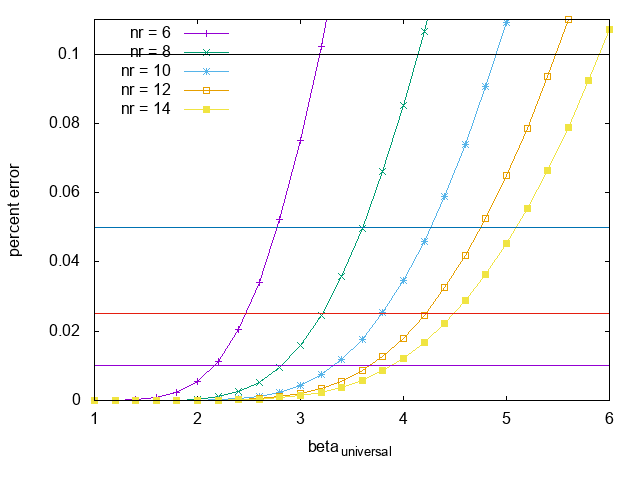
\includegraphics[width=0.6\textwidth]{error}
    \caption{Percent error of the 0D Hartree self energy versus $\beta_{\mathrm{universal}}$ for different radial grid sizes.} 
    \label{fig:error}
\end{figure}

\begin{figure}[!htbp] 
    \centering
    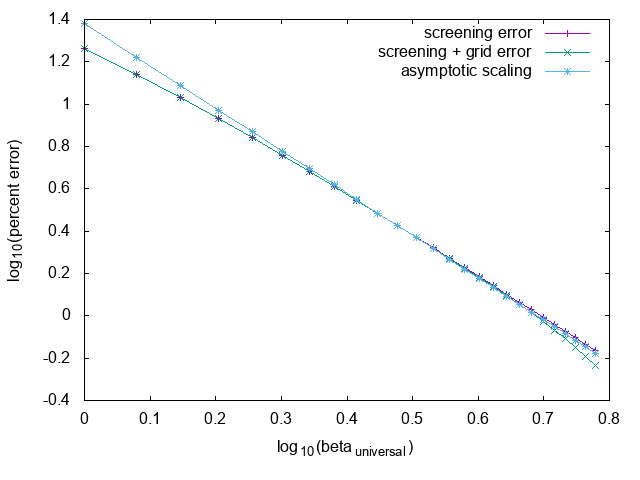
\includegraphics[width=0.6\textwidth]{diffbeta}
    \caption{For $n_r = 14$, the percentage difference between the screened and unscreened 0D Hartree self energy term versus $\beta_{\mathrm{universal}}$. The asymptotic regime is reached for $\beta_{\mathrm{universal}} > 2$.} 
    \label{fig:diffbeta}
\end{figure}

\begin{figure}[!htbp] 
    \centering
    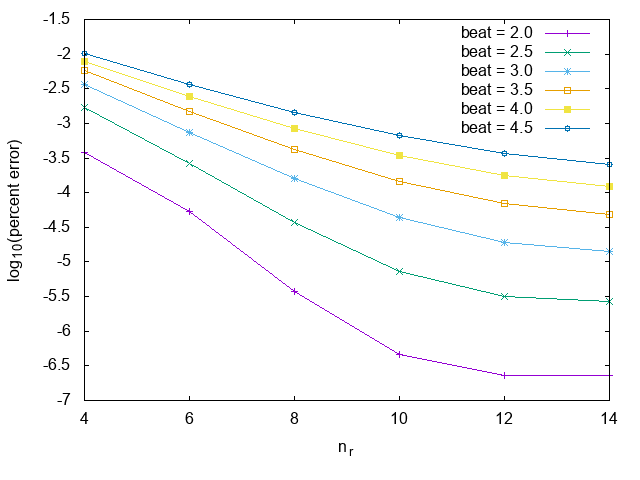
\includegraphics[width=0.6\textwidth]{betaconv}
    \caption{Percentage error of the 0D Hartree self energy versus $n_r$ for different $\beta_{\mathrm{universal}}$ on a semilog plot.} 
    \label{fig:diffbeta}
\end{figure}

\begin{figure}[!htbp] 
    \centering
    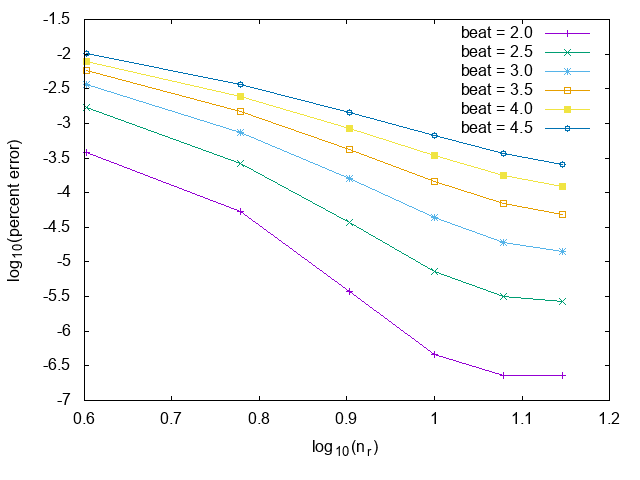
\includegraphics[width=0.6\textwidth]{betaconvloglog}
    \caption{Percentage error of the 0D Hartree self energy versus $n_r$ for different $\beta_{\mathrm{universal}}$ on a loglog plot.} 
    \label{fig:diffbeta}
\end{figure}

\begin{figure}[!htbp] 
    \centering
    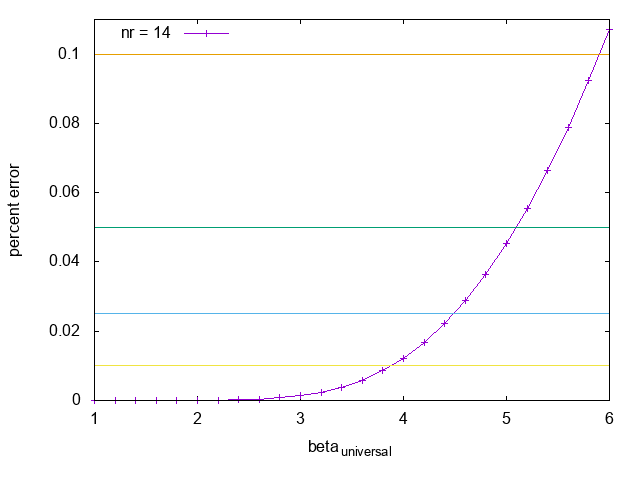
\includegraphics[width=0.6\textwidth]{error3D}
    \caption{Percent error of the 3D Hartree short self energy versus $\beta_{\mathrm{universal}}$ for $n_r = 14$.} 
    \label{fig:error3D}
\end{figure}

\begin{figure}[!htbp] 
    \centering
    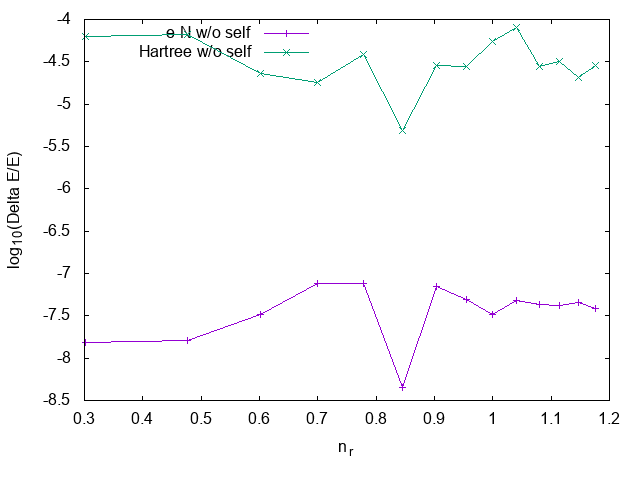
\includegraphics[width=0.6\textwidth]{conv}
    \caption{The fractional error between the grid and analytical 0D e-N energy and Hartree energy without the self term versus $n_r$.} 
    \label{fig:conv0D}
\end{figure}

\begin{figure}[!htbp] 
    \centering
    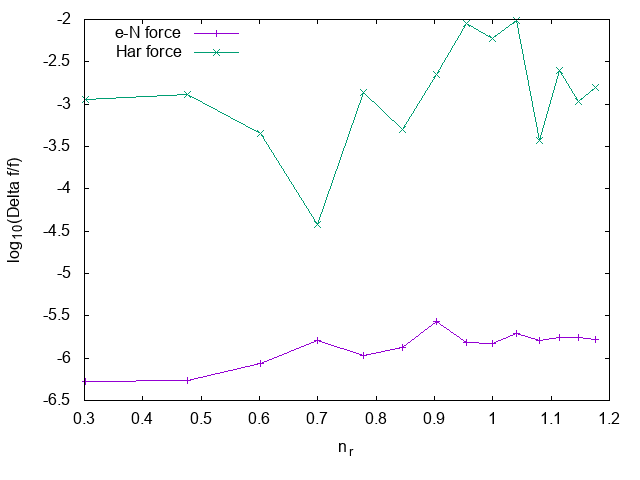
\includegraphics[width=0.6\textwidth]{fconv}
    \caption{The fractional error between the grid and analytical 0D e-N force and Hartree force versus $n_r$.} 
    \label{fig:fconv0D}
\end{figure}

\subsection{3D screened Hartree self term}
\begin{equation}
\begin{split}
E^{(\rcomp)} 
&= \frac{1}{2}\sum_\bm \iint_{D(\bh)} \rd \br \rd \br' \frac{n^{(\rcomp)}(\br)n^{(\rcomp)}(\br')\left[1-1+\rerf(\beta|\br-\br'+\bm\bh|)\right]}{|\br-\br'+\bm\bh|} - E_{\rNN}^{(\rself)}\\
&= \frac{1}{2}\sum_\bm \iint_{D(\bh)} \rd \br \rd \br' \frac{\left[\rerfc(\bal |\br-\br'+\bm\bh|)- \rerfc(\beta|\br-\br'+\bm\bh|) \right]n^{(\rcomp)}(\br)n^{(\rcomp)}(\br')}{|\br-\br'+\bm\bh|} - E_{\rNN}^{(\rself,\rshort)} \\
&+ \frac{1}{2}\sum_\bm \iint_{D(\bh)} \rd \br \rd \br' \frac{\rerf(\bal |\br-\br'+\bm\bh|)n^{(\rcomp)}(\br)n^{(\rcomp)}(\br')}{|\br-\br'+\bm\bh|} - E_{\rNN}^{(\rself,\rlong)} \\
\end{split}
\end{equation}

Only the short Hartree term is modified, because $\beta$ is chosen very large to screen the Coulomb interaction only inside the PAW radius $-$ the Coulomb interaction between 2 different PAW spheres will not be screened. The condition is $\beta \Rpc >> 1$, while $\bal$ has the more relaxed condition $\bal \Rc >> 1$, where $\Rc > \Rpc$ as described in section 1, page 3. $\Rpc \approx 3/(\sqrt{2}\al)$ for our Gaussian compensation charge. In our tests, $\beta/\al \approx 4$.

\begin{equation}
\begin{split}
E^{(\rcomp,\rshort)} 
&= \frac{1}{2}\iint \rd \br \rd \br' \frac{n^{(\rcomp)}(\br)n^{(\rcomp)}(\br')\left[\rerfc(\bar {\al}|\br-\br'|) - \rerfc(\beta|\br-\br'|)\right]} {|\br-\br'|} - E_{\rNN}^{(\rself,\rshort)}\\
&= \frac{1}{2}\iint \rd \br \rd \br' \frac{\rerfc(\bar {\al}|\br-\br'|) - \rerfc(\beta|\br-\br'|)}{|\br-\br'|}{|\br-\br'|} \left[\sum_J Z_J\delta(\br-\bR_J) - \sum_J \tilde Z_J\left(\frac{\al_J^2}{\pi}\right)^{\frac{3}{2}}\re^{-\al_J^2|\br-\bR_J|^2}\right]\\
&\hspace{10mm}\times \left[\sum_K Z_K\delta(\br'-\bR_K) - \sum_K \tilde Z_K\left(\frac{\al_K^2}{\pi}\right)^{\frac{3}{2}}\re^{-\al_K^2|\br'-\bR_K|^2}\right] - E_{\rNN}^{(\rself,\rshort)}\\
&= \frac{1}{2}\iint \rd \br \rd \br' \frac{\rerfc(\bar {\al}|\br-\br'|) - \rerfc(\beta|\br-\br'|)}{|\br-\br'|} \left\{\sum_J \sum_{K \neq J} Z_J Z_K \delta(\br-\bR_J)\delta(\br'-\bR_K) \right. \\
&\left.\hspace{10mm} - \sum_J Z_J\delta(\br-\bR_J) \sum_K \tilde Z_K\left(\frac{\al_K^2}{\pi}\right)^{\frac{3}{2}}\re^{-\al_K^2|\br'-\bR_K|^2} \right. \\
&\left.\hspace{10mm} - \sum_J Z_K\delta(\br'-\bR_J) \sum_J \tilde Z_J\left(\frac{\al_J^2}{\pi}\right)^{\frac{3}{2}}\re^{-\al_J^2|\br-\bR_J|^2} \right. \\
&\left.\hspace{10mm} + \sum_J\sum_K \tilde Z_J\tilde Z_K\left(\frac{\al_J\al_K}{\pi}\right)^3\re^{-\al_J^2|\br-\bR_J|^2-\al_K^2|\br'-\bR_K|^2}\right\}\\
&= \frac{1}{2}\iint \rd \br \rd \br' \frac{\rerfc(\bar {\al}|\br-\br'|)}{|\br-\br'|} \left\{\sum_J \sum_{K \neq J} Z_J Z_K \delta(\br-\bR_J)\delta(\br'-\bR_K) \right. \\
&\left.\hspace{10mm} - \sum_J Z_J\delta(\br-\bR_J) \sum_K \tilde Z_K\left(\frac{\al_K^2}{\pi}\right)^{\frac{3}{2}}\re^{-\al_K^2|\br'-\bR_K|^2} \right. \\
&\left.\hspace{10mm} - \sum_J Z_K\delta(\br'-\bR_J) \sum_J \tilde Z_J\left(\frac{\al_J^2}{\pi}\right)^{\frac{3}{2}}\re^{-\al_J^2|\br-\bR_J|^2} \right. \\
&\left.\hspace{10mm} + \sum_J\sum_K \tilde Z_J\tilde Z_K\left(\frac{\al_J\al_K}{\pi}\right)^3\re^{-\al_J^2|\br-\bR_J|^2-\al_K^2|\br'-\bR_K|^2}\right\}\\
&- \frac{1}{2}\iint \rd \br \rd \br'\frac{\rerfc(\beta|\br-\br'|)}{|\br-\br'|} \left\{ \sum_J \tilde Z_J^2\left(\frac{\al_J^2}{\pi}\right)^3\re^{-\al_J^2|\br-\bR_J|^2-\al_J^2|\br'-\bR_J|^2}\right\}\\
&= \frac{1}{2}\sum_{J} \sum_{K \neq J} \frac{\rerfc(\bal R_{JK})Z_JZ_{K}}{R_{JK}}  - \sum_J \sum_{K \neq J} \tilde Z_J Z_K \frac{\rerfc(\bal_J R_{JK}) - \rerfc(\al_J R_{JK})}{R_{JK}}  \\
&\hspace{10mm}+ \frac{1}{2}\sum_J\sum_{K \neq J} \tilde Z_J \tilde Z_K  \frac{\rerfc(\bal_{JK} R_{JK}) - \rerfc(\al_{JK} R_{JK})}{R_{JK}} + E^{(\rcomp,\rshort,\rself, \mathrm{scr})} \\
\end{split}
\end{equation}

Since different atom types can have different screening factor, we construct
\begin{equation}
\beta_J = \beta_{\mathrm{unitless}} \al_J
\end{equation}
where $\beta_{\mathrm{unitless}}$ is a universal factor for all atom types.


\begin{equation}
\begin{split}
E^{(\rcomp,\rshort,\rself, \mathrm{scr})} 
&= E^{(\rcomp,\rshort,\rself)} - \frac{1}{2}\sum_J \tilde Z_J^2  \left(\frac{\al_J^2}{\pi}\right)^3 \left\{ \iint \rd \br \rd \br' \frac{\rerfc(\beta_J|\br-\br'|)}{|\br-\br'|} \re^{-\al_J^2|\br-\bR_J|^2-\al_J^2|\br'-\bR_J|^2}\right\}\\
&= E^{(\rcomp,\rshort,\rself)} - \frac{1}{2}\sum_J \tilde Z_J^2  \left(\frac{\al_J^2}{\pi}\right)^3 \left\{ \iint \rd \br \rd \br' \frac{1}{|\br-\br'|} \re^{-\al_J^2|\br-\bR_J|^2-\al_J^2|\br'-\bR_J|^2}\right\} \\
& \hspace{5mm} +\frac{1}{2}\sum_J \tilde Z_J^2  \left(\frac{\al_J^2}{\pi}\right)^3 \left\{ \iint \rd \br \rd \br' \frac{\rerf(\beta_J|\br-\br'|)}{|\br-\br'|} \re^{-\al_J^2|\br-\bR_J|^2-\al_J^2|\br'-\bR_J|^2}\right\}\\
&= E^{(\rcomp,\rshort,\rself)} - \frac{1}{2}\sum_J \tilde Z_J^2  \left(\frac{\al_J^2}{\pi}\right)^3 \left\{ \iint \rd \br \rd \br' \frac{1}{|\br-\br'|} \re^{-\al_J^{2} r^2-\al_J^{2} r'^{2}}\right\} \\
& \hspace{5mm} +\frac{1}{2}\sum_J \tilde Z_J^2  \left(\frac{\al_J^2}{\pi}\right)^3 \left\{ \iint \rd \br \rd \br' \frac{\rerf(\beta_J|\br-\br'|)}{|\br-\br'|} \re^{-\al_J^{2} r^{2} - \al_J^{2} r'^{2}}\right\}\\
&= E^{(\rcomp,\rshort,\rself)} - \lim_{\gamma \rightarrow 0} \frac{1}{2}\sum_{J}  \tilde Z_J^2 \frac{\rerf(\al_{J}\gamma)}{\gamma} + \lim_{\gamma \rightarrow 0} \frac{1}{2} \sum_J \tilde Z_J^2 \frac{\rerf(\beta_{J}\gamma)}{\gamma} \\
&= E^{(\rcomp,\rshort,\rself)} + \sum_J \tilde Z_J ^2 \frac{\bar{\beta}_{JJ} - \al_{JJ} }{\sqrt{\pi}}
\end{split}
\end{equation}

where
\begin{equation}
\bar{\beta}_{JJ}= \frac{\beta_J \al_J^2}{\sqrt{\al_J^4 + 2\beta_J^2\al_J^2 }}
\end{equation}

\newpage
\section{Charged systems under 3D periodic boundary conditions}\label{App:c3D}
The standard treatment of charged systems under 3D periodic boundary conditions simply subtracts out the uniform neutralizing background energy - the infinite energy of the constant charge density.\\

A more refined treatment is to add the constant neutralizing background explicitly to the charge density and compute
\begin{equation}\label{eq:m1}
\begin{split}
E^{(\mathrm{electrostatic-neutral})}
&= \frac{1}{2}\int_{\rD(\bh)} \rd \br \int_{\rD(\bh)}\rd \br'\sum_\bm \frac{\left[n(\br)-\rho^{(\mathrm{neutral})}\right]\left[n(\br')-\rho^{(\mathrm{neutral})}\right]}{|\br-\br'+\bm\bh|} - E_{\rNN}^{(\rself)}\\
\end{split}
\end{equation}
where 
\begin{equation}
\begin{split}
\int_{\rD(\bh)} \rd \br\ n(\br) &= Q \\
\rho^{(\mathrm{neutral})} &= \frac{Q}{V}
\end{split}
\end{equation}
and $E_{\rNN}^{(\rself)}$ is the infinity energy of any point sources in the charge density from interaction in the 1st image.\\

Expanding Eq.\eqref{eq:m1},
\begin{equation}
\begin{split}
E^{(\mathrm{electrostatic-neutral})}
&= \frac{1}{2}\int_{\rD(\bh)} \rd \br \int_{\rD(\bh)}\rd \br'\sum_\bm \frac{\left[n(\br)n(\br')-2\rho^{(\mathrm{neutral})}n(\br) + \left(\rho^{(\mathrm{neutral})}\right)^2\right]}{|\br-\br'+\bm\bh|} - E_{\rNN}^{(\rself)}\\
\end{split}
\end{equation}
The 1st term is the energy we normally calculate, the 2nd term is new, and the 3rd term is the background which we evaluated in Appendix \ref{App:Compc}, and only contributes at $\bg = 0$. Moving forward, 
\begin{equation}
\begin{split}
E^{(\mathrm{electrostatic-neutral})}
&= \frac{1}{2}\int_{\rD(\bh)} \rd \br \int_{\rD(\bh)}\rd \br'\sum_\bm \frac{n(\br)n(\br')}{|\br-\br'+\bm\bh|} - E_{\rNN}^{(\rself)} \\
&- \int_{\rD(\bh)} \rd \br \int_{\rD(\bh)}\rd \br'\sum_\bm \frac{\rho^{(\mathrm{neutral})}n(\br)}{|\br-\br'+\bm\bh|} \\
&+ \frac{1}{2}\int_{\rD(\bh)} \rd \br \int_{\rD(\bh)}\rd \br'\sum_\bm \frac{\left(\rho^{(\mathrm{neutral})}\right)^2}{|\br-\br'+\bm\bh|} \\
&= \frac{1}{2}\int_{\rD(\bh)} \rd \br \int_{\rD(\bh)}\rd \br'\sum_\bm \frac{n(\br)n(\br')}{|\br-\br'+\bm\bh|} - E_{\rNN}^{(\rself)} \\
&- \frac{Q^2}{V}\lim_{\bg \rightarrow 0} \frac{4\pi}{g^2}\\
&+ \frac{Q^2}{2V} \lim_{\bg \rightarrow 0} \frac{4\pi}{g^2}\\
\end{split}
\end{equation}
where
\begin{equation}
\begin{split}
\int_{\rD(\bh)} \rd \br \int_{\rD(\bh)}\rd \br'\sum_\bm \frac{\left[\rho^{(\mathrm{neutral})}n(\br)\right]}{|\br-\br'+\bm\bh|}
&= \frac{\rho^{(\mathrm{neutral})}}{V} \sum_{\bg} \frac{4\pi}{g^2}\int_{\rD(\bh)}\rd \br\ n(\br) e^{-i\bg\cdot \br} \int_{\rD(\bh)} \rd \br'  e^{-i\bg\cdot \br'}\\
&= \frac{\rho^{(\mathrm{neutral})}}{V} \sum_{\bg} \frac{4\pi}{g^2} \bar n(\bg) V \delta_{\bg,0} \\
&= \rho^{(\mathrm{neutral})} \bar n(0)\lim_{\bg \rightarrow 0} \frac{4\pi}{g^2}  \\
&= \frac{Q^2}{V}\lim_{\bg \rightarrow 0} \frac{4\pi}{g^2} \\
\end{split}
\end{equation}

Therefore,
\begin{equation}\label{eq:m6}
\begin{split}
E^{(\mathrm{electrostatic-neutral})}
&= \frac{1}{2}\int_{\rD(\bh)} \rd \br \int_{\rD(\bh)}\rd \br'\sum_\bm \frac{n(\br)n(\br')}{|\br-\br'+\bm\bh|}- E_{\rNN}^{(\rself)}  - \frac{Q^2}{2V} \lim_{\bg \rightarrow 0} \frac{4\pi}{g^2} \\
\end{split}
\end{equation}
The $\bg = 0$ contribution of the 1st term on the RHS is 
\begin{equation}
\frac{Q^2}{2V} \lim_{\bg \rightarrow 0} \frac{4\pi}{g^2}
\end{equation}
and the neutralizing background cancels all divergences at $\bg = 0$.\\

To prove the $\bg = 0$ behavior of the 1st term we introduce Poisson summation to the 1st term of Eq.\eqref{eq:m6}, and it is simple to show that the result is
\begin{equation}
\begin{split}
\frac{\left|\bar n(0)\right|^2}{2V}\lim_{\bg \rightarrow 0} \frac{4\pi}{g^2}
&= \frac{Q^2}{2V} \lim_{\bg \rightarrow 0} \frac{4\pi}{g^2} 
\end{split}
\end{equation}
Hence, we just throw away the background and do not care about carrying around $\rho^{(\mathrm{neutral})}$ in our calculations. This is the way Appendix \ref{App:Compc} is done.\\

We have to be careful not to neglect non-vanishing $\bg = 0$ terms. For example, we should really write
\begin{equation}
\frac{1}{2V}\lim_{\bg \rightarrow 0} \frac{4\pi}{g^2} \left|\bar n(\bg)\right|^2
\end{equation}
which for a Gaussian charge distribution, 
\begin{equation}
\begin{split}
\frac{1}{2V}\lim_{\bg \rightarrow 0} \frac{4\pi}{g^2} \left|\bar n(\bg)\right|^2
&= \frac{Q^2}{2V}\lim_{\bg \rightarrow 0}\frac{4\pi}{g^2} \rexp\left(-\frac{g^2}{2\al^2}\right)\\
&= \frac{Q^2}{2V}\lim_{\bg \rightarrow 0}\frac{4\pi}{g^2} -\frac{Q^2 \pi}{V \al^2}
\end{split}
\end{equation}
The leading over term is the singularity that gets cancelled, but the 2nd term is non-zero and needs to be included (there is nothing to cancel it).
\\

Orthogonality of spherical harmonics
\begin{equation}
\begin{split}
\int_{-1}^1 \rd u \int_{0}^{2\pi} \rd \phi Y_{lm}(u,\phi)Y_{l'm'}^*(u,\phi)
&= \int_{-1}^1 \rd u \int_{0}^{2\pi} \rd \phi C_{lm} P_l^m(u)\re^{im\phi}C_{l'm'} P_{l'}^{m'}(u)\re^{-im'\phi}\\
&= C_{lm}C_{l'm'} \int_{-1}^1 \rd u P_l^m(u) P_{l'}^{m'}(u) \int_{0}^{2\pi} \rd \phi\re^{im\phi}\re^{-im'\phi}\\
&= C_{lm}C_{l'm} \int_{-1}^1 \rd u P_l^m(u) P_{l'}^{m}(u)  \delta_{mm'}\\
&= \delta_{ll'}\delta_{mm'}
\end{split}
\end{equation}

but
\begin{equation}
C_{lm}C_{l'm'} \int_{-1}^1 \rd u P_l^m(u) P_{l'}^{m'}(u)
\neq \delta_{ll'}
\end{equation}
unless $m = m'$.

There is a simple grid in ($u, \phi$) that yields exactly orthogonality of the spherical harmonics for a given $l_{\mathrm{max}}$ and $|m_{\mathrm{max}}| = l_{\mathrm{max}}$. The phi integral can be performed on an equally spaced grid of size $n_{\phi} > 2l_{\mathrm{max}}$. This will provide the $\delta_{mm'}$ for $m$ and $m'$ in the specified range. For $m=m'$, $P_{l}^{m}(u)P_{l'}^{m}(u)$ is a polynomial of degree $2l$. Therefore, the $u$ integral will be exact for Gauss-Legendre quadrature with $n_u >= l_{\mathrm{max}}$. 

\newpage
\section{Generalized Gaussian Quadrature Integration}\label{App:GGI}
The goal is to develop quadratures for integration of polynomials over a positive semidefinite weighting function.
\begin{equation}
\begin{split}
I &= \int_{a}^{b}w(x) f(x) \\
I &\approx I_n = \sum_{i=0}^{n-1} w_i^{(n)} f(x_i^{(n)})
\end{split}
\end{equation}
where $I_n$ is exact for $f(x)$ a polynomial of degree $2n-1$. It has been shown that given a set of orthogonal polynomials $p_n(x)$ over the weighting function $w(x)$, selecting the $x_i^{(n)}$ to be the roots of $p_n(x)$, and the weights to be
\begin{equation}
\begin{split}
w_{i}^{(n)}={\frac {a_{n}^{(n)}}{a_{n-1}^{(n)}}}{\frac {\int _{a}^{b}\omega (x)p_{n-1}(x)^{2}dx}{p'_{n}(x_{i}^{(n)})p_{n-1}(x_{i}^{(n)})}}
\end{split}
\end{equation}
yields the desired result.
Here, the $p'_{n}(x)$ is the derivative w.r.t $x$ of the polynomial $p_n(x)$, and the $a_n^{(n)}$ is the coefficient of the $n^{\mathrm{th}}$ power of the $x$ in the polynomial.\\

In order to evaluate the expression for the weights, we first assume we can perform integrals of polynomials over the weighting function analytically. Second, it is then a simple matter to construct the coefficients of an orthogonal polynomial using Gram-Schmidt orthogonalization. Third, given the ${\bf a}^{(n)}$'s from the Gram Schmidt process, we can obtain the weights from the eigenvalues of the companion matrix.
\begin{equation}
\det \left({\bf A}_n- {\bf I} x\right) = p_n(x)
\end{equation}
and hence, the eigenvalues of ${\bf A}_n$ are the zeros of $p_n(x)$. The companion matrix has zeros everywhere except the last column, which are the $-{\bf a}^{(n)}/a_n^{(n)}$ and the $A_{i+1,i} = 1$.
Thus, finding zeros is reduced to finding the eigenvalues of the companion matrix, which we can do with any linear algebra packages (in lapack: DGGEV).\\


We begin the formal development by writing the orthogonal polynomials $p_n(x)$ over the weighting function $w(x)$ in the $x^k$ basis set as:
\begin{equation}
\begin{split}
p_n(x)  &= \sum_{k=0}^n a_{nk} x^k \\
p'_{n}(x) &= \sum_{k=1} k a_{nk} x^{k-1}\\
\int_a^b \rd x w(x) p_m(x) p_n(x) &= \delta_{mn} N_{nn} \\
\end{split}
\end{equation}
The parameter $a_{nn}$ can be selected to have unit norm, $N_{nn} = 1$, or set to unity, $a_{nn} = 1$, with non-trivial norm. We shall show how to develop the $a_{nk}$ using a Gram-Schmidt procedure given knowledge of
\begin{equation}
I_k = \int_a^b \rd x w(x) x^k\ \ \ \ k = 0\ldots 2n
\end{equation}

In order to proceed, we recognize that we can expand the $k$'th order orthogonal polynomial in terms of the lower order polynomials $j = 0 \ldots k-1$
\begin{equation}
p_k(x)  = \sum_{j=0}^{k-1} p_{j}(x) c_{kj} + c_{kk} x^k
\end{equation}
with the $c_{kj}$ the expansion coefficients. As above, we are free to choose $c_{kk} = 1$ and a non-trivial norm, or unit norm and a non-trivial $c_{kk}$. Note the $c-$matrix is lower triangular

\[ 
\left [
  \begin{tabular}{cccc}
  $1$ & $0$ & ... & $0$ \\
  $c_{10}$ & 1 & ... & $0$ \\
  ... & ... & ... & $0$\\
  $c_{n0}$ & ... & ... & $1$\\
  \end{tabular}
\right ]
\]

Next, we prove by induction that a Gram-Schmidt procedure can be used to construct the $c_{kj}$'s. Assuming that we have all the $c_{ij}$ for $i = 0\ldots k-1$ and the $I_{k}$'s, we show we can construct the $c_{kj}$ such that $p_k(x)$ is orthogonal to all polynomials $p_j(x), j = 0\ldots k-1$,
\begin{equation}
\begin{split}
\int_a^b \rd x w(x) p_k(x) p_j(x) 
&= \int_a^b \rd x w(x) \left[\sum_{i=0}^{k-1} p_{i}(x) c_{ki} + c_{kk} x^k\right] p_i(x) =0 \\
&= \sum_{i=0}^{k-1} \int_a^b \rd x w(x) p_{i}(x) p_j(x) c_{ki} + c_{kk}\int_a^b \rd x w(x) x^k p_j(x)=0 \\
&= \sum_{j=0}^{k-1} c_{ki} N_{ii} \delta_{ij} + c_{kk} O_{kj}=0\\
&= N_{jj} c_{kj} + c_{kk} O_{kj}=0\\
\end{split}
\end{equation}

which leads to
\begin{equation}
c_{kj} = -\frac{c_{kk} O_{kj}}{N_{jj}}\ \ \ \
j = 0\ldots k-1
\end{equation}
Here,
\begin{equation} 
O_{kj} = \int_a^b \rd x w(x) x^k p_j(x) = \sum_{l=0}^j a_{jl} I_{k+l}
\end{equation}
which can be evaluated using the $a-$ representation of $p_j(x)$. \\

Alternatively, the $O_{kj}$ can be evaluated recursively using the $c-$ representation. Assuming the $O_{kl}\ \ k = 0 \ldots n, \ l = 0 \ldots j-1$, it is possible to construct $O_{kj}$ as
\begin{equation}
\begin{split}
O_{kj} &= \int_a^b \rd x w(x) x^k p_j(x) \\
&= \int_a^b \rd x w(x) x^k  \left[\sum_{l=0}^{j-1} p_{l}(x) c_{jl} + c_{jj} x^j\right]\\
&= \sum_{l=0}^{j-1} c_{jl} \int_a^b \rd x w(x) x^k p_{l}(x) + c_{jj}\int_a^b \rd x w(x) x^k x^j \\
&= \sum_{l=0}^{j-1} c_{jl}O_{kl} + c_{jj} I_{k+j}
\end{split}
\end{equation}

Next, we connect the $c$ representation to the $a$ representation recursively by induction.
Assuming the $a_{jl}$ for $j = 0 \ldots k-1$ are known,   
\begin{equation}
\begin{split}
p_k(x) &= \sum_{j=0}^{k-1} p_{j}(x) c_{kj} + c_{kk} x^k \\
&= \sum_{j=0}^{k-1} \sum_{l=0}^j a_{jl} x^l c_{kj} + c_{kk} x^k \\
&= \sum_{l=0}^{k-1} x^l \sum_{j=l}^{k-1} a_{jl} c_{kj} + c_{kk} x^k \\
&= \sum_{l=0}^{k-1} x^l a_{kl} + a_{kk} x^k \\
\end{split}
\end{equation}
the $a_{kl}$ are hence
\begin{equation}
\begin{split}
a_{kl} &= \sum_{j=l}^{k-1} a_{jl} c_{kj} \ \ \ l=0 \ldots k-1 \\
a_{kk} &= c_{kk}
\end{split}
\end{equation}

It is possible to express the companion matrix in terms of the $c$'s instead of the $a$'s. This maybe desirable for large $n$ as the $c$ representation may have a lower condition number. For now we will forgo this pleasure.

We now consider the norm,
\begin{equation}
\begin{split}
N_{nn} &= \int_a^b \rd x w(x) p_n(x) p_n(x) \\
&= \int_a^b \rd x w(x) \left[\sum_{j=0}^{n-1} p_{j}(x) c_{nj} + c_{nn} x^n\right] \left[\sum_{k=0}^{n-1} p_{k}(x) c_{nk} + c_{nn} x^n\right] \\
&= \int_a^b \rd x w(x) \left\{\sum_{j=0}^{n-1} \sum_{k=0}^{n-1} p_{j}(x) c_{nj}p_{k}(x) c_{nk} + 2c_{nn} x^n \sum_{j=0}^{n-1} p_{j}(x) c_{nj} + c_{nn}^2 x^{2n}\right\} \\
&= \sum_{j=0}^{n-1} \sum_{k=0}^{n-1} c_{nj}c_{nk}\int_a^b \rd x w(x) p_{j}(x)p_{k}(x) + 2c_{nn}  \sum_{j=0}^{n-1} c_{nj} \int_a^b \rd x w(x) p_{j}(x)x^n + c_{nn}^2 \int_a^b \rd x w(x) x^{2n} \\
&= \sum_{j=0}^{n-1} c_{nj}^2 N_{jj} + 2c_{nn}  \sum_{j=0}^{n-1} c_{nj} O_{nj} + c_{nn}^2 I_{2n}
\end{split}
\end{equation}

If we desire to work with unit norm, we can use $c_{nn}$ to renormalize all our coefficients as all are scaled by $c_{nn}$.
\begin{equation}
\begin{split}
c_{nj} &= \frac{c_{nj}^{(0)}}{\sqrt{N_{nn}^{(0)}}}\ \ \ \ j = 0 \ldots n \\
\end{split}
\end{equation}
where $c_{nj}^{(0)}$ is Eq. (N.8) with $c_{nn} = 1$, and $N_{nn}^{(0)}$ is Eq. (N.13) also with $c_{nn} = 1$.

We next treat Gaussian weights over the full space
\begin{equation}
\begin{split}
I_k &= \int_{-\infty}^{\infty} \rd x \re^{-ax^2} x^k\ \ \ \ k = 0,2,\ldots 2n \\
I_k &= 0\ \ \ \ k = 1,3,\ldots 2n-1 \\
\end{split}
\end{equation}
In order to treat the even case, we use the following parametric derivative trick:
\begin{equation}
\begin{split}
I_{2k} &= (-1)^k \frac{\rd ^{k}}{\rd a^k} \int_{-\infty}^{\infty} \rd x \re^{-a x^2}= \int_{-\infty}^{\infty} \rd x \re^{-ax^2} x^{2k}\\
&= (-1)^k \frac{\rd ^{k}}{\rd a^k} \sqrt{\frac{\pi}{a}}
\end{split}
\end{equation}

The generalized form is:
\begin{equation}
\begin{split}
I_{2k} &= \sqrt{\pi} \frac{1\cdot 3 \cdot \ldots \cdot (2k-1)}{2^k}a^{-\frac{2k+1}{2}}\\
I_{2k+2} &= I_{2k}\frac{(2k+1)}{2a}
\end{split}
\end{equation}

For the half space, the even guys just get a half. The odd guys we make the transformation

\begin{equation}
\begin{split}
I_{2k+1} &= \int_{0}^{\infty} \rd x\ \re^{-ax^2} x^{2k+1}\ \ \ \ k = 0,\ldots n-1 \\
&= \frac{1}{2}\int_{0}^{\infty} \rd u\ \re^{-au} u^k \\
&= \frac{(-1)^k }{2} \frac{\rd ^{k}}{\rd a^k}\int_{0}^{\infty} \rd u\ \re^{-au} \\
&= \frac{(-1)^k }{2} \frac{\rd ^{k}}{\rd a^k} \frac{1}{a}\\
&= \frac{k!}{2} a^{-(k+1)}\\
I_{2k+3} &= I_{2k+1} (k+1)a^{-1}
\end{split}
\end{equation}

\section{Scratch paper}
The integral in L.63
\begin{equation}
\begin{split}
&\frac{-\re^{-(a^2 -1) x^2} + \re^{-(a^2 + 1) x^2} +\sqrt{\pi}\sqrt{(a^2 -1)x^2}\rerfc\left(\sqrt{(a^2 -1)x^2}\right) - \sqrt{\pi}\sqrt{(a^2 +1)x^2}\rerfc\left(\sqrt{(a^2 +1)x^2}\right) }{2x} \mid_0^{\beta\sqrt{2rr'}} \nonumber
\end{split}
\end{equation}
where
\begin{equation}
\begin{split}
a^2 &= \frac{r^2 + r'^2}{2rr'} \geq 1 \\
x &\geq 0
\end{split}
\end{equation}

Next, we evaluate the lower limit
\begin{equation}
\begin{split}
\frac{\sqrt{\pi}}{2}\left(\sqrt{a^2 -1} - \sqrt{a^2 + 1}\right)
&= \frac{\sqrt{\pi}}{2}\left(\sqrt{\frac{r^2 + r'^2}{2rr'} -1} - \sqrt{\frac{r^2 + r'^2}{2rr'} + 1}\right)\\
&= \frac{\sqrt{\pi}}{2\sqrt{2r_>r_<}} \left(r_> - r_< - r_> - r_<\right)\\
&= -\frac{r_<}{\sqrt{2r_>r_<}} \\
&= -\sqrt{\frac{\pi r_<}{2r_>}} \\
\end{split}
\end{equation}

In order to take the upper limit, we first simplify some terms,
\begin{equation}
\begin{split}
(a^2 - 1)x^2
&= (r-r')^2 \beta^2 \\
(a^2 + 1)x^2
&= (r+r')^2 \beta^2 \\
\end{split}
\end{equation}

\begin{equation}
\begin{split}
&\frac{-\re^{-\beta^2(r-r')^2 } + \re^{-\beta^2(r+r')^2 } +\sqrt{\pi}\sqrt{(r-r')^2 \beta^2}\rerfc\left(\sqrt{(r-r')^2 \beta^2}\right) - \sqrt{\pi}\sqrt{(r+r')^2 \beta^2}\rerfc\left(\sqrt{(r+r')^2 \beta^2}\right) }{2\beta \sqrt{2 r r'}} \\
&= \frac{-\re^{-\beta^2(r-r')^2 } + \re^{-\beta^2(r+r')^2 }}{2\beta \sqrt{2 r r'}} + \frac{\sqrt{\pi}(r_> - r_<)\rerfc\left(\beta(r_> - r_<)\right) - \sqrt{\pi}(r_> + r_<)\rerfc\left(\beta(r_> + r_<)\right)}{2\sqrt{2rr'}}\\
&= \frac{-\re^{-\beta^2(r-r')^2 } + \re^{-\beta^2(r+r')^2 }}{2\beta \sqrt{2 r r'}} + \frac{\sqrt{\pi}(r_> - r_<)\rerfc\left(\beta(r_> - r_<)\right) - \sqrt{\pi}(r_> + r_<)\rerfc\left(\beta(r_> + r_<)\right)}{2\sqrt{2rr'}} \nonumber
\end{split}
\end{equation}

Combining the two terms yields
\begin{equation}
\begin{split}
&\frac{-\re^{-\beta^2(r-r')^2 } + \re^{-\beta^2(r+r')^2 }}{2\beta \sqrt{2 r r'}} + \frac{\sqrt{\pi}(r_> - r_<)\rerfc\left(\beta(r_> - r_<)\right) - \sqrt{\pi}(r_> + r_<)\rerfc\left(\beta(r_> + r_<)\right)}{2\sqrt{2rr'}} + \sqrt{\frac{ \pi r_<}{2r_>}}
\end{split}
\end{equation}
the prefactor from L.63 is
\begin{equation}
\sqrt{\frac{2}{\pi r r'}} 
\end{equation}

Multiplying through, we obtain
\begin{equation}
\frac{\re^{-\beta^2(r_>+r_<)^2 }-\re^{-\beta^2(r_>-r_<)^2 }}{2\beta \sqrt{\pi}r_> r_< } + \frac{(r_> - r_<)\rerfc\left(\beta(r_> - r_<)\right) - (r_> + r_<)\rerfc\left(\beta(r_> + r_<)\right)}{2 r_>r_<} + \frac{1}{r_>}
\end{equation}

\newpage
\section{Spherical Bessel Compensation Charge Model}\label{App:SBC}
For spherical charge density, we write the compensation charge in terms of spherical Bessel functions
\begin{equation}
\begin{split}
n^{(\rcomp)}(\br) 
&= \sum_J Z_J\delta(\br-\bR_J) - \sum_J n_J^{(\rcore)}(\br)\\
&= \sum_J Z_J\delta(\br-\bR_J) - \sum_J \tilde Z_J \frac{2 \left|j_0(k_J r)\right|^2}{R_{\mathrm{pc},J}} Y_{00}\left(\cos(\theta),\phi\right)
\end{split}
\end{equation}
where
\begin{equation}
\begin{split}
j_0(k_J r) &= \frac{\sin(k_J r)}{r} \\
k_J &= \frac{\pi \hat {k}}{R_{\mathrm{pc},J}},\ \ \ \ \hat {k} = \mathrm{integer} > 0
\end{split}
\end{equation}

The first advantage of the spherical Bessel function is that we need not truncate the expansion at a single $\hat {k}$ if we desire a more accurate compensation charge because the $j_0$'s form a complete orthonormal set on the closed interval (0, $\Rpc$). This is simply done by replacing the single spherical Bessel in P.1 by a sum, 

\begin{equation}
j_0(k_J r) \rightarrow \sum_{\hat {k} = 1}^{\hat {k}_{\mathrm{max}}} c_{\hat {k}}j_0(k_J r)
\end{equation}
and changing the normalization as well.
\begin{equation}
\frac{2}{R_{\mathrm{pc},J}} \rightarrow \frac{2}{R_{\mathrm{pc},J}\sum_{\hat {k} = 1}^{\hat {k}_{\mathrm{max}}} |c_{\hat {k}}|^2}
\end{equation}

The second advantage is that for a finite set of $\hat {k} \leq \hat {k}_{\mathrm{max}}$, an equally spaced grid in $r$ assures orthogonality in the finite space of $\hat {k}_{\mathrm{max}}$ (just like for planewave expansions). The number of points in $r$ is just greater than $2\hat {k}_{\mathrm{max}} + 1$, 
\begin{equation}
\begin{split}
\int_0^{R_{\mathrm{pc},J}} \rd r r^2 j_0(k_J r) j_0(k'_J r)
&= \int_0^{R_{\mathrm{pc},J}} \rd r \sin(k_J r) \sin(k'_J r) = \frac{2}{R_{\mathrm{pc},J}}\\
&= \Delta \sum_{i=0}^{n_r} \sin(k_J r_i) \sin(k'_J r_i) 
\end{split}
\end{equation}

where
\begin{equation}
\begin{split}
\Delta &= \frac{R_{\mathrm{pc},J}}{n_r} \\
r_i &= \Delta \hat {i}
\end{split}
\end{equation}

The third advantage is that the weight and nodes of the grid are simple.

We can evaluate the model analytically, but we will try it first numerically and look at the convergence.

We tested the Bessel grid for $\hat {k}_{\mathrm{max}} = 1$ using the screened and unscreened Hartree self term. The results indicate that the non-analytical character of the unscreened reduces the power law convergence from $n_r^4$ to $n_r^2$.

\begin{figure}[!htbp] 
    \centering
    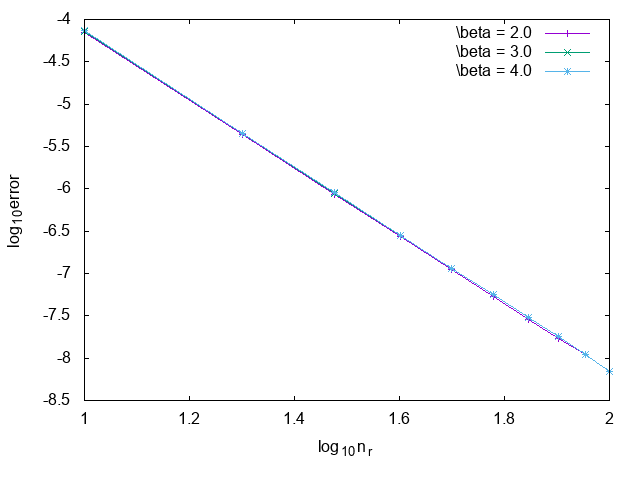
\includegraphics[width=0.6\textwidth]{sBesselerror}
    \caption{The convergence of the screened Hartree self term for the spherical Bessel basis with $\hat {k}_{\mathrm{max}} = 1$ versus $n_r$.} 
    \label{fig:sBesselerror}
\end{figure}

\begin{figure}[!htbp] 
    \centering
    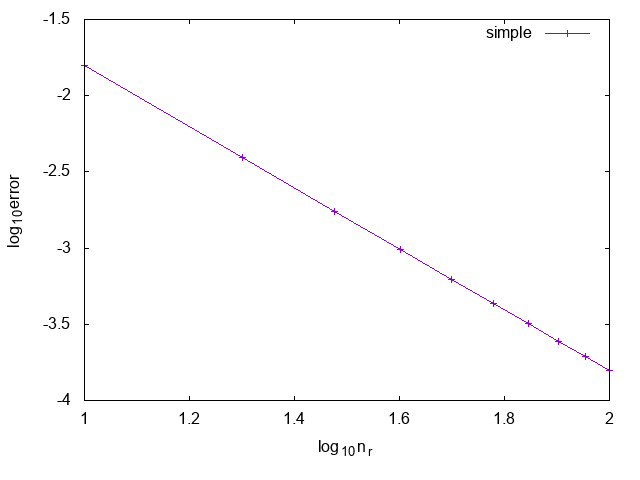
\includegraphics[width=0.6\textwidth]{sBesselerrorsimple}
    \caption{The convergence of the unscreened Hartree self term for the spherical Bessel basis with $\hat {k}_{\mathrm{max}} = 1$ versus $n_r$.} 
    \label{fig:sBesselerrorsimple}
\end{figure}

\begin{figure}[!htbp] 
    \centering
    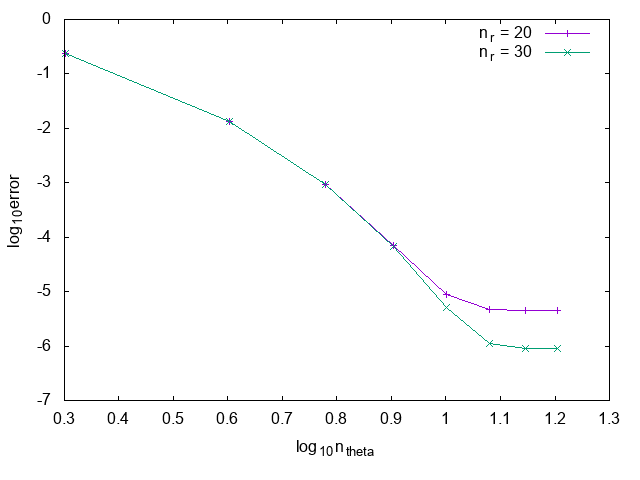
\includegraphics[width=0.6\textwidth]{nthetaHarself}
    \caption{The convergence of the screened Hartree self term for the spherical Bessel basis with $\hat {k}_{\mathrm{max}} = 1$ versus $n_{\theta}$. Here, $n_r = 20$, $n_{\phi} = 2n_{\theta}$.} 
    \label{fig:nthetaHarself}
\end{figure}

In Fig.\ref{fig:nthetaHarself}, we compare the convergence of the partial wave expansion and the full integral over the angular momentum for an s-wave spherical Bessel wavefunction $\hat {k}_{\mathrm{max}} = 1$. Although the convergence to the s-wave result is exponential in the number of angular points, it is pretty wasteful. That means grinding out a few more terms in the partial wave expansion of the screened Hartree self is a good idea.

\begin{figure}[!htbp] 
    \centering
    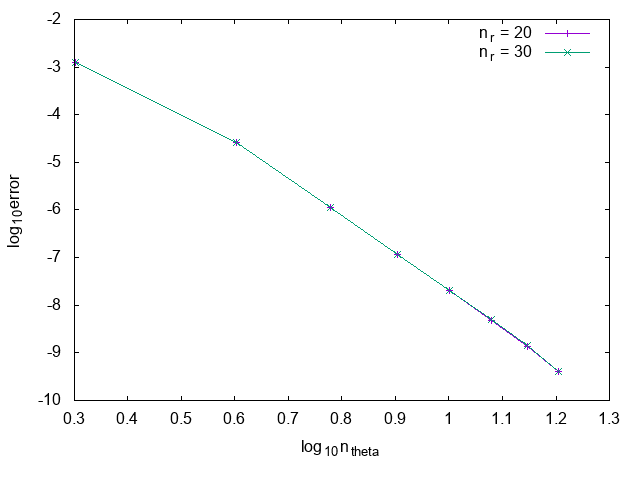
\includegraphics[width=0.6\textwidth]{nthetaHarwoself}
    \caption{The convergence of the unscreened Hartree term (self term excluded) for the spherical Bessel basis with $\hat {k}_{\mathrm{max}} = 1$ versus $n_{\theta}$. Here, we study $n_r = 20$ and $n_r = 30$, using $n_{\phi} = 2n_{\theta}$. Here, $n_{\theta} = 20$, $n_{\phi} = 40$ are used as the ``correct answer'' for the 2 values of $n_r$.} 
    \label{fig:nthetaHarwoself}
\end{figure}

\begin{figure}[!htbp] 
    \centering
    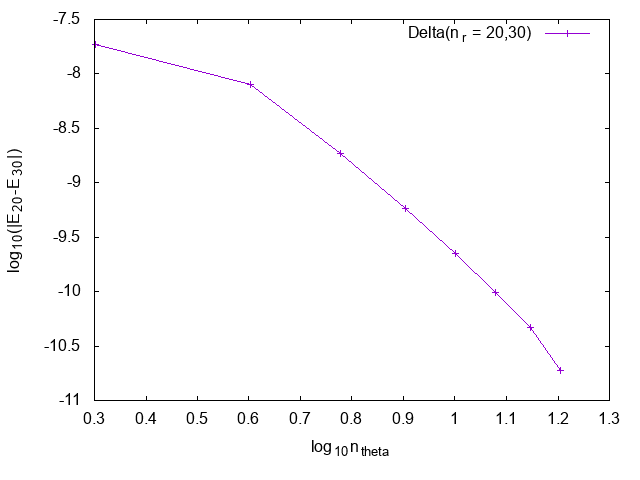
\includegraphics[width=0.6\textwidth]{nthetaHarwoselfdiff}
    \caption{The difference between the Hartree no self term of $n_r = 20$ and $n_r = 30$. The difference is always small.} 
    \label{fig:nthetaHarwoselfdiff}
\end{figure}

\begin{figure}[!htbp] 
    \centering
    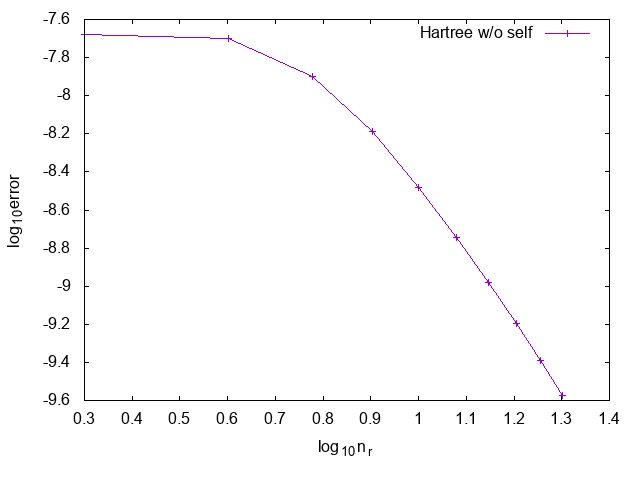
\includegraphics[width=0.6\textwidth]{nrHarwoself}
    \caption{The convergence of the unscreened Hartree term (self term excluded) for the spherical Bessel basis with $\hat {k}_{\mathrm{max}} = 1$ versus $n_r$. Here, $n_{\theta} = 10$, $n_{\phi} = 20$.} 
    \label{fig:nrHarwoself}
\end{figure}

From Fig.P.1 where we looked at the convergence of the screened Hartree self term using s-wave only, we see that for $n_r = 10$ we achieve 4 figures accuracy. The slope of the curve is -4 indicating 4th order convergence. Therefore, to achieve 6 figures accuracy, we need 30 points while 20 points achieve 5 figures. In Fig.P.2, we look at unscreened Hartree, which converges terribly - only 2nd order.\\

In Fig.P.3, we examine the convergence of the screened Hartree self term without the partial wave expansion. To achieve the $n_r$ limited accuracy, $n_{\theta} = 12$ with $n_{\phi} = 24$. The conclusion here is we should use the partial wave expansion to limit the size of the angular grid.


\end{document}